\documentclass[a4paper]{jreport}
\newcommand{\version}{5.0.1}

\title{{\vspace{2cm}{\Large Version \version} }}
\author{\Large Team SCALE\\ UGC working group}
\date{\today}


\usepackage[dvipdfmx]{graphicx, color}
\usepackage[dvipdfmx]{hyperref}
\usepackage{amsmath}
\usepackage{ascmac}
\usepackage{alltt}
\usepackage[round]{natbib}
\usepackage{tabularx}
\usepackage{color}
\usepackage{colortbl}
\usepackage{fancybox}
\usepackage{url}
\usepackage{longtable}
\usepackage{pxjahyper}
\usepackage{comment}
\hypersetup{% options for hyperref
 bookmarksopen=true,
 bookmarksnumbered=true,
 colorlinks=true,
% linkcolor=red,
 linkcolor=cyan,
 citecolor=cyan,
 urlcolor=cyan,
}

\makeatletter
\@addtoreset{chapter}{part}
\makeatother

%\setlength{\textwidth}{42zw}
%\setlength{\textheight}{40\baselineskip}
\usepackage[top=30mm,bottom=35mm,left=30mm,right=30mm]{geometry}
\usepackage{wallpaper}
%\renewcommand{\thefootnote}{\fnsymbol{footnote}}
\renewcommand{\thefootnote}{*\arabic{footnote})}
\renewcommand{\thepart}{\arabic{part}}
\renewcommand{\thechapter}{\arabic{part}.\arabic{chapter}}
\renewcommand{\prechaptername}{}
\renewcommand{\postchaptername}{}
\newcommand{\namelist}[1]{{\color{magenta}\texttt{[\detokenize{#1}]}}}
\newcommand{\nmitem}[1]{{\color{magenta}\texttt{(\detokenize{#1})}}}
\newcommand{\XDIR}{X方向}
\newcommand{\YDIR}{Y方向}
\newcommand{\ZDIR}{Z方向}
%%%%
%%%% for chapter 5
\newcommand{\SecBasicDomainSetting}{{対象計算領域の設定}}
\newcommand{\SubsecRelationOfResoGridProcess}{{計算領域と解像度、格子点数、MPIプロセスの関係}}
\newcommand{\SubsecDomainSetting}{{計算領域の設定}}
\newcommand{\SubsecMPIProcess}{{MPIプロセス数}}
\newcommand{\SubsecGridNumSettng}{{水平・鉛直格子数の設定}}
\newcommand{\SubsecGridIntvSettng}{{水平・鉛直格子間隔の設定}}
\newcommand{\SecBasicBufferSetting}{{緩和領域の設定}}
\newcommand{\SecBasicTopoSetting}{{地形の設定}}
\newcommand{\SecBasicIntegrationSetting}{{積分時間と積分時間間隔の設定}}
\newcommand{\SecBasicOutputSetting}{{出力変数の追加・変更方法}}
\newcommand{\SecBasicDynamicsSetting}{{力学スキームの設定}}
\newcommand{\SubsecDynsolverSetting}{{数値解法の設定}}
\newcommand{\SubsecDynSchemeSetting}{{時間・空間差分スキームの設定}}
\newcommand{\SecBasicPhysicsSetting}{{物理スキームの設定}}
\newcommand{\SubsecMicrophysicsSetting}{{雲微物理スキームの設定}}
\newcommand{\SubsecTurbulenceSetting}{{乱流スキームの設定}}
\newcommand{\SubsecRadiationSetting}{{放射スキームの設定}}
\newcommand{\SubsecSurfaceSetting}{{地表面(大気下端境界)の設定}}
\newcommand{\SubsecOceanSetting}{{海洋モデルの設定}}
\newcommand{\SubsecLandSetting}{{陸面モデルの設定}}
\newcommand{\SubsecUrbanSetting}{{都市モデル(大気-都市面フラックス)の設定}}

%%%%
%%%% for chapter 6
\newcommand{\SecAdvanceMapprojectionSetting}{{地図投影法と計算領域の位置の設定}}
\newcommand{\SecAdvanceInputDataSetting}{{様々な初期値・境界値データを使用する}}
\newcommand{\SecAdvanceRestart}{{リスタート計算の方法}}



\begin{document}
\CenterWallPaper{1.0}{figure/title_wallpaper.eps}
\maketitle
\ClearWallPaper
\ULCornerWallPaper{.1}{figure/scale_logo_final_ULWB.eps}
\tableofcontents

%-----------------------------------------------------------------------
% Part and chapter are defined in this main tex file.
% Sections are defined in each input tex file.
%-----------------------------------------------------------------------

\part{概要} \label{part:overview}
 \chapter{はじめに} \label{sec:introduction}
 
%==============================================================%

本書は初めて領域気象気候モデル {\scalerm}
を利用する人に向けた解説書である。
気象気候ライブラリー{\scalelib}  version \version に対応した説明を記載する。
\scalelib の現バージョンには、領域モデル\scalerm と全球モデル\scalegm が含まれる。
本版では、\scalerm の使い方についてのみ詳しく述べる。
\scalegm については、次版で詳しく記載される予定である。
%\scalerm の使い方を通して、\scalelib を他のモデルからの呼び出す方法を
%習得することも可能です。

本書の構成は次の通りです。
第\ref{part:overview}部では SCALE の概要、
第\ref{part:install}部では必要な環境とインストール方法について説明する。
続いて、第\ref{chap:tutorial_ideal}章では理想実験、第\ref{chap:tutorial_real}章では現実大気実験を例にして、\scalerm の基本的な操作方法を説明する。
これらの章はひと繋がりのチュートリアルとなっており、
\scalerm を初めて使うユーザは一通り通読することを推奨する。
第\ref{part:basic_usel}部と第\ref{part:advance_use}部では、
モデルの設定の変更方法を記載し、また利用できるデータ形式やツールを説明する。
これらの各章は基本的にその中で閉じているので、辞書として用いることができる。

%%%
本書中の不明点やお気づきの点がございましたら、SCALE user's メーリングリスト\\
 \verb|scale-users@ml.riken.jp|までご連絡ください。



\section{\scalelib とは?} \label{subsec:scale_feature}
%--------------------------------------------------------------%

{\scalelib} (Scalable Computing for Advanced Library and Environment)は、
気候研究や天気予報を容易に様々な計算機上で行うためのソフトウェア・ライブラリである。
本ライブラリは、前処理からシミュレーション、後処理、解析に至るまで全ての過程を網羅し、
下記に挙げる長所を持つ。
\begin{itemize}
\item \scalelib は、「BSD-2ライセンス」のもとオープンソースソフトウェア
として提供している。
商用、非商用に関わらず自由な利用、改変、再配布が可能である。
\item \scalelib には、{\scalerm} (SCALE-Regional Model)
%SCALE-GM(SCALE-Global Model)
という領域モデルが含まれる。
\item \scalelib には、次節で説明するように様々なスキームが用意されている。
ユーザーが行いたい実験に合わせて適宜選択できる。
\item \scalelib では、\scalerm だけでなく他の数値モデルでも呼び出せる
物理過程のフレームワークを提供している。
\end{itemize}

ライセンスの詳細は、トップディレクトリ直下の\texttt{scale-\version/LICENSE}のファイルに記述されている。
\scalelib の使用前に一読されたい。
また、\scalelib のWebページ(\url{http://scale.aics.riken.jp/})にもソフトウェアの説明が記載されているので必要に応じて参照されたい。

本節では、\scalelib の思想や実際のモデルとの関係について説明する。
\scalerm の実行とは直接的には関係しないため、必要なければ読み飛ばしても構わない。

\Item{\scalelib のライブラリとモデルの関係について}

\begin{figure}[htb]
\begin{center}
  \includegraphics[width=0.9\hsize]{./figure/library_jp.eps}\\
  \caption{\scalelib のねらい}
  \label{fig:scale}
\end{center}
\end{figure}

\scalelib は幾つかの外部共同研究者と共に理化学研究所(RIKEN)で開発され、
その改良と拡張が継続的に行われている。
図 \ref{fig:scale}に\scalelib の思想の概念図を示す。
この図に示されるように、\scalelib は様々な問題に対応することを目指している。
\scalelib は、小型PCクラスターから次世代のスーパーコンピュータに至るまで様々な計算環境で広く用いられる事を念頭に開発されている。
この目的のため、気候・気象科学を専門とする科学者と計算機科学を専門とする科学者が
共同で開発している。

\scalerm は \scalelib ライブラリを大いに利用した数値モデルの一つであり、
図\ref{fig:scale-rm}に示すように \scalelib のパッケージに含まれる。
\scalelib は、並列プロセスの管理、ファイルの入出力、プロセス間の通信、格子情報の設定を行う。
また、\scalelib は、大気の流れのソルバ(力学コア)や雲微物理や大気放射等の物理過程も提供する。
その一方で、\scalerm は\scalelib が提供する機能を組み合わせることで構築されている。
\scalerm 自体は、大気の状態の入力データを予報変数として読み込んで保持し、
\scalelib の各コンポーネントを適宜呼び出すことで時間発展を計算する。
ユーザは行いたい実験に応じて、各コンポーネントのスキームを選択できる。

\begin{figure}[hbt]
\begin{center}
  \includegraphics[width=0.9\hsize]{./figure/scale_jp.eps}\\
  \caption{{\scalelib}ライブラリと{\scalerm}(モデル)の関係}
  \label{fig:scale-rm}
\end{center}
\end{figure}



\section{\scalerm の構成}  \label{subsec:sturcture_scale_rm}
%--------------------------------------------------------------%
\scalelib に含まれる全てのコンポーネント中の全てのスキームを、
\scalerm において利用できる。
コンポーネントは3つの部分(フレームワーク、力学コア、物理過程)に分類される。
以下に、\scalerm の現版に実装済みである、様々なスキームを含むコンポーネントを列挙する%
\footnote{
モデルの構成や離散化法の詳細は、
\citet{scale_2015}、\citet{satoy_2015b}、
\citet{nishizawa_2015}を参照されたい。
}。
\\

{\bf フレームワーク}
\begin{itemize}
 \item 実距離に基づいた3次元カーテシアン格子系
 \item MPI通信を用いた2次元領域分割
 \item 各種地図投影法
 \item 領域ネスティングシステム(1 way:親領域$\to$子領域へデータ転送)
   \begin{itemize}
    \item オンライン・ネスティング: 複数ドメインの計算を同時に実行
    \item オフライン・ネスティング:外側ドメインの計算終了後に、その結果を用いて内側ドメインの計算を実行
   \end{itemize}
 \item 複数事例一括実行システム(バルクジョブシステム)
 \item CF 規約\footnote{\url{http://cfconventions.org/}}に基づく \netcdf ファイル I/O
   \begin{itemize}
   \item {\netcdf}3 または {\netcdf}4 形式を選択
   \end{itemize}
 \item 理想実験のための初期値データ生成
 \item 外部データから標高・土地利用区分データを作成
 \item 外部データから初期値・境界値データを作成
   \begin{itemize}
    \item
      WRF-ARW\footnote{\url{http://www.wrf-model.org/}}、
%      NICAM\footnote{\url{http://nicam.jp/}}、
      \grads \footnote{\url{http://cola.gmu.edu/grads/}}形式での入力に対応
   \end{itemize}
\end{itemize}

{\bf 力学コア}
\begin{itemize}
 \item 支配方程式系: 3次元完全圧縮非静力学方程式系
 \item 空間離散化: 有限体積法
    \begin{itemize}
      \item 2次, 4次, 6次中央差分
      \item 3次, 5次風上差分
    \end{itemize}
 \item 時間離散化: 「完全陽解法」または「水平陽解法-鉛直陰解法」から選択
    \begin{itemize}
      \item Heun型3次ルンゲ・クッタスキーム
      \item \citet{Wicker_2002}の3段ルンゲ・クッタスキーム
      \item 4次ルンゲ・クッタスキーム
    \end{itemize}
 \item 非負保証:
    \begin{itemize}
      \item フラックス修正法 \citep[Flux Corrected Transport, FCT; ][]{zalesak_1979}
      \item \citet{Koren_1993}フィルター  (3次風上差分スキーム使用時のみ)
    \end{itemize}
 \item 数値フィルタ: 4次超粘性・拡散
 \item 地形: 地形に沿った座標系を用いて表現
\end{itemize}

{\bf 物理過程}
\begin{itemize}
 \item 乱流過程: 以下から選択可能
   \begin{itemize}
    \item \citet{smagorinsky_1963} \& \citet{lilly_1962}型のサブグリッドスケール乱流モデル (\citet{Brown_etal_1994}と\citet{Scotti_1993}による補正)
    \item \citet{Deardorff_1980} サブグリッドスケール乱流モデル
    \item \citet{my_1982,nakanishi_2004}によるlevel 2.5境界層乱流パラメタリゼーション
   \end{itemize}
 \item 雲微物理: 以下から選択可能
   \begin{itemize}
    \item \citet{kessler_1969}による3-class 1モーメントバルクモデル
    \item \citet{tomita_2008}による6-class 1モーメントバルクモデル
    \item \citet{sn_2014}による6-class 2モーメントバルクモデル
    \item \citet{suzuki_etal_2010}によるビン法モデル
   \end{itemize}
 \item 放射過程: \citet{sekiguchi_2008}による相関k分布法ブロードバンド大気放射伝達モデル
 \item 地表面モデル
  \begin{itemize}
   \item 陸面モデル: 熱拡散・バケツモデル
   \item 海洋モデル: 以下から選択可能
   \begin{itemize}
     \item 初期値固定
     \item 外部データ入力
     \item スラブモデル
   \end{itemize}
   \item 都市モデル: \citet{kusaka_2001}による単層キャノピーモデル
   \item バルク交換係数(陸面および海面): 以下から選択可能
   \begin{itemize}
     \item \citet{beljaars_1991,wilson_2001}による普遍関数によるバルク法
     \item \citet{uno_1995}によるLouis 型バルク法
   \end{itemize}
  \end{itemize}
\end{itemize}

 \chapter{表記上の注意} \label{sec:notation}
 
This document assumes an execution in the shell ``bash'' on some Unix system.
If your environment is different, replace the commands
by the relevant commands suitable for your environment.
Unless there is a particular remark, this documentation obeys the following notation:

The command-line symbol for execution is expressed by \verb|$| or \verb|#|.
The difference between the two notations is
in the permission levels of program execution, as shown below:
\begin{verbatim}
 #        <- command by root permission
 $        <- command by user permission
\end{verbatim}

A description enclosed in a rectangle expresses a message generated by the command line, as shown below.
\msgbox{
 -- -- -- -- command-line message\\
 -- -- -- -- -- -- -- -- command-line message\\
 -- -- -- -- -- -- -- -- -- -- -- -- command-line message\\
}

On the other hand, a description enclosed in a rounded rectangle shows a part of configuration file including namelists, which can be edited as needed.
\editbox{
 -- -- -- -- description in a file\\
 -- -- -- -- -- -- -- -- description in a file\\
 -- -- -- -- -- -- -- -- -- -- -- -- description in a file\\
}

In this documentation, the FORTRAN namelist and its items are denoted by
\namelist{namelist} and \nmitem{item_of_namelist}, respectively.



\part{インストール} \label{part:install}
 \chapter{準備}
 This chapter explains how to compile \scalelib / \scalerm
and the minimum computational requirements for their execution.

\section{System environment} \label{sec:req_env}
%====================================================================================
\subsubsection{Recommended Hardware}

  Although the necessary hardware depends on the experiment to be performed,
the following are the specifications for conducting a tutorial as in Chapters \ref{chap:tutorial_ideal} and \ref{chap:tutorial_real}.

  \begin{itemize}
    \item {\bf CPU} :
    The system need to have more than two and more than four physical cores
    for an ideal experiment and a real atmospheric experiment, respectively.
    \item {\bf Memory} :
    The system needs 512 MB and 2 GB memory
    for the ideal experiment and a real atmospheric experiment, respectively.
    Note that this applies to the case involving the use of double-precision floating points.
    \item {\bf HDD} : The system needs to have 3 GB of free disk space in a real atmospheric experiment.
  \end{itemize}


\subsubsection{Required Software}

  \begin{itemize}
  \item {\bf OS} : Linux OS, Mac OS X
  %Refer to Table \ref{tab:compatible_os} for other OSs currently supported.
  \item {\bf Compiler} : C, Fortran
  \end{itemize}

Since the source code of \scalelib is  written in FORTRAN 2003 standard syntax, the compiler must support it. For example, GNU gfortran version 4.3 or previous versions cannot be used for \scalelib compilation because they do not follow the FORTRAN 2003 standard. Refer to Table \ref{tab:compatible_compiler} for compilers already confirmed as supported.

In addition to the above environment, it has been confirmed that \scalelib can be compiled and run on  machines with a SPARC-based instruction set, such as the K Computer.


\begin{table}[tb]
\begin{center}
\caption{Compiler already checked}
\begin{tabularx}{150mm}{|l|X|} \hline
 \rowcolor[gray]{0.9} Name of compiler &  \\ \hline
  GNU (gcc/gfortran)    & Version 4.3 or earlier are not supported. The series with version 4.4.x sometimes issues a warning. \\ \hline
  Intel (icc/ifort)     & Version of 2013 or later are recommended. \\ \hline
  PGI (gcc/pgfortran)   & Version 17.1 is comfirmed.       \\ \hline
\end{tabularx}
\label{tab:compatible_compiler}
\end{center}
\end{table}



\subsubsection{Required libraries}\label{sec:inst_env}

The required external libraries are described below; each library is commonly used.
\begin{itemize}
\item HDF5 Library (\url{https://www.hdfgroup.org/HDF5/})
\item {\netcdf} Library (\url{http://www.unidata.ucar.edu/software/netcdf/})
\item MPI Library (openMPI version、\url{http://www.open-mpi.org/})
\item LAPACK ( \url{http://www.netlib.org/lapack/} ) (only required for \scalegm)
\end{itemize}


The MPI library should support the MPI 1.0/2.0 protocol.  Refer to Table \ref{tab:compatible_mpi} for MPI libraries already confirmed as supported.
%
The libraries of gzip, HDF5, and {\netcdf}4 are required. In stead of the HDF5/{\netcdf}4, {\netcdf}3 is sufficient, but the size of the output file increases in this case.
The information about installation of each library is provided from the above URLs.;
you can also use distributed packages for Linux and Mac. 
These libraries have been already installed on the K Computer as AICS software. Refer to the description ``AICS software'' in the K portal site or the URL\\ \url{https://www-sys-aics.riken.jp/releasedsoftware/ksoftware/pnetcdf/}\\ for details. The library paths are described there in ``Makedef.K.'' The tutorials in Chapters \ref{chap:tutorial_ideal} and \ref{chap:tutorial_real} assume that the above library environment has been prepared.



\begin{table}[tb]
\begin{center}
\caption{Compiler list}
\begin{tabularx}{150mm}{|l|X|} \hline
 \rowcolor[gray]{0.9} Name of MPI library &  \\ \hline
  openMPI               & Version 1.7.2 or later is supported. \\ \hline
  Intel MPI             & Version released in 2013 or later is supported.\\ \hline
  SGI MPT               & Version 2.09 or later is supported. \\ \hline
\end{tabularx}
\label{tab:compatible_mpi}
\end{center}
\end{table}






\subsubsection{Drawing tools}

The following are typical drawing tools that can draw
the initial conditions, boundary data, and the simulation results on \scalelib.
The GPhys and \grads are used for a quick view
and the drawing model output in the tutorial in Chapters \ref{chap:tutorial_ideal} and \ref{chap:tutorial_real}, respectively.
Other tools are of course available,
if they can be read in \netcdf format, which is the output format of \scalelib.

\begin{itemize}
\item GPhys / Ruby-DCL by GFD DENNOU Club
 \begin{itemize}
  \item URL: \url{http://ruby.gfd-dennou.org/products/gphys/}
  \item Note: \scalelib outputs the split files
  in {\netcdf} format according to domain decomposition by the MPI process.
  "gpview" and/or "gpvect" in {\gphys} can directly draw the split file without post-processing.
  \item How to install:
  On the GFD DENNOU Club webpage, the installation is explained for major OSs\\
  \url{http://ruby.gfd-dennou.org/tutorial/install/}\\
  %\url{https://www.gfd-dennou.org/library/ruby/tutorial/install/index-j.html}\\
   \end{itemize}
\item Grid Analysis and Display System (\grads) by COLA
 \begin{itemize}
  \item URL: \url{http://cola.gmu.edu/grads/}
  \item Note:This is among the most popular drawing tools,
  but the split files with {\netcdf} generated by \scalelib are not directly readable.
  The post-processing tool \verb|netcdf2grads_h| is needed to combine the output of \scalelib in one file that is readable from \grads. Refer to \verb|netcdf2grads_h| for installation instructions in Section \ref{sec:source_net2g}, and to Chapters 3 and 4 and Section \ref{sec:net2g} for details pertaining to its use.
  \item How to install: Refer to \url{http://cola.gmu.edu/grads/downloads}.
 \end{itemize}
\item Ncview: {\netcdf} visual browser developed by David W. Pierce
 \begin{itemize}
  \item URL: \url{http://meteora.ucsd.edu/~pierce/ncview_home_page.html}
  \item Note: Ncview is a quick viewer for the {\netcdf} file format.
  Although it cannot combine split files in \scalelib, it is useful in drawing the result file by file.
  \item How to install: Refer to \url{http://meteora.ucsd.edu/~pierce/ncview_home_page.html}
 \end{itemize}
\end{itemize}


\subsubsection{Useful tools (not always necessary)}
\begin{itemize}
  \item {\bf Data conversion tool}: wgrib, wgrib2, NCL\\
  In the tutorial for the real atmospheric experiment, wgrib is used.
  \item {\bf Evaluation tool of computational performance}:The PAPI library\footnote{\url{http://icl.utk.edu/papi/}} is available.
\end{itemize}


 \chapter{\scalelib のコンパイル}
 \section{Installation of SCALE-LES}
%####################################################################################

本章では,日本域を対象とした現実大気再現実験のチュートリアルを通して,
SCALE-LESモデルを実行する一連の作業を説明する.
SCALEライブラリのインストールに必要な環境、ライブラリのインストール方法については,
\ref{sec:req_env}節とAppendix \ref{sec:env_setting}を参照して
事前にインストールしておく必要がある.
\ref{sec:source_code}以降のチュートリアルは,それらのライブラリ環境が
インストールされていることを想定して進める.


\subsection{Required Environment}
\label{sec:req_env}
%====================================================================================

\begin{itemize}
  \item {\bf 計算機環境} : Unix互換OS (Mac OS Xを含む)が動作する環境.
        マルチコアCPU環境以上を推奨する.
        実験サイズによるが4GB以上のメモリがインストールされているマシン環境が好ましい.
  \item {\bf OS} : Linux OS(Fedora, CentOS, SUSE等),Mac OS X.ここではLinux (CentOS6)を使用して説明する.
  \item {\bf コンパイラ} : Fortran 2003をサポートするC,Fortranコンパイラを必要とする.
        GNU 4.6.x以上,Intel compiler 2012以上を推奨する.ここでは,gcc/gfortranを使用して説明する.
  \item {\bf MPIライブラリ} : MPICH2, OpenMPI, Intel MPI等をサポートする.ここではopenMPIを使用して説明する.
  \item {\bf netcdf3 もしくは HDF5/netcdf4} : gzip, szipをサポートするHDF5,
        およびそのHDF5をサポートするnetcdf4を必要とする.
        ただし,netcdf3の環境下ではscaleライブラリが提供する全ての機能をサポートできない可能性がある.
  \item {\bf 描画環境(非必須)} : Dennou Club提供のRuby DCL/GPhysに含まれるgpviewがあると
        計算結果を簡単にチェックできる.チュートリアルではgpviewを使用する.
        それ以外に,netcdfからGrADS用にフォーマットを変換するためのpostprocess(\verb|netcdf2grads_h|)も用意している.
  \item SCALEは演算性能評価のためにPAPIライブラリを使用が可能.
        PAPIライブラリがインストールされている環境下では,
        以下で説明するconfigureファイルの編集によってPAPIを適用することができます.
\end{itemize}


\subsection{Building the source code} \label{sec:source_code}
%====================================================================================

\subsubsection{ソースコードの入手}
%-----------------------------------------------------------------------------------

安定版ソースコードは,\url{http://scale.aics.riken.jp/ja/download/index.html}
よりダウンロードすることができる.
ソースコードのtarballファイルを展開すると
\begin{verbatim}
  scale/
\end{verbatim}
というディレクトリができる.

現実大気実験のシミュレーションを行う場合,SCALE本体に加えて境界値データが必要になる.
本チュートリアル用の気象場のデータ,日本領域の地形・土地利用のデータを\\
 \url{http://scale.aics.riken.jp/download/tutorial_data.tar.gz}\\
より入手し,チュートリアルの入力ファイル用ディレクトリ
\begin{verbatim}
  scale/scale-les/test/tutorial/data/
\end{verbatim}
の下に展開しておく.

以降の説明で\verb|${TOPDIR}|は,\verb|scale/scale-les/test/tutorial/|がある絶対PATHを指す.

\begin{verbatim}
  ${TOPDIR}/data/tutorial_data/input_atom/    <- 気象場データ
  ${TOPDIR}/data/tutorial_data/input_topo/    <- 地形データ
  ${TOPDIR}/data/tutorial_data/input_landuse/ <- 土地利用データ
\end{verbatim}
\verb|tutorial_data/|には,本チュートリアルに必要な最低限のデータのみが納めされているため,
その他の設定で実験を行う場合には別途,気象場,地形,および土地利用データが必要となる.


\subsubsection{configure ファイルと環境変数の設定}
%-----------------------------------------------------------------------------------

\verb|scale/sysdep/|内にいくつかのコンフィグファイル(\verb|Makedef.***|)が準備されている.
これらの中から自分の環境にあったものを設定する.
ここでは,OSはLinux,コンパイラはgcc/gfortran,およびopenMPIを使用するため,
\verb|"Makedef.Linux64-gnu-ompi"|が対応するファイルとなる.
自分の環境に合うものがなければ既存ファイルをベースにして作成する.

常にこのコンフィグファイルをしようするために、
\verb|Makedef.***|の\verb|"***"|の部分を、\verb|SCALE_SYS|という環境変数として設定し、
\verb|.bashrc|などのファイルに記述しておくと便利である.
さらに、SCALEをコンパイルするのに必要な外部ライブラリについても
下記のようにPATHを設定する.
ここでは,Appendix \ref{sec:env_setting}に従ったとして,
HDF5,netcdf4ともに\verb|/usr|の下にインストールされている場合の例を示す.

\begin{verbatim}
 $ export SCALE_SYS="Linux64-gnu-ompi"
 $ export HDF5="/usr"
 $ export NETCDF4="/usr"
\end{verbatim}


\subsubsection{コンパイル}
%-----------------------------------------------------------------------------------

下記のディレクトリに移動して,makeコマンドによってコンパイルを行う.
\begin{verbatim}
 $ cd ${TOPDIR}/bin
 $ make -j 4
\end{verbatim}
\verb|make|のあとの \verb|"-j 4"| は,並列コンパイルを指示するオプションで,
4並列コンパイルを行うことを指示している.
コンパイルを実行する環境によっては並列数を増やすこともできる.
このmakeによってSCALEライブラリ,およびSCALE-LESモデルのコンパイルが行われ,
結果として
\begin{verbatim}
 scale-les  scale-les_init  scale-les_pp
\end{verbatim}
の3つの実行ファイルが生成されていればコンパイルは成功である.\\


{\bf 注意点}
\begin{itemize}
\item SCALEライブラリは,scaleのTOPディレクトリ直下の
 \verb|scale/scalelib/|というディレクトリ内でコンパイルとアーカイブが行われ,
 \verb|".lib"|という名前の隠しディレクトリとして
 \verb|bin/|ディレクトリ内へコピーされている.
\item Debugモードでコンパイルしたい場合や,
 コンパイルオプションを変更したい場合は,
 \verb|Makedef.***|のファイルを編集してください.
\item 開発版ソースコードをコンパイルしている場合,
 一部のコンパイラバージョンにおいてコンパイルが正常に終了しないケースがあります.そのような場合はぜひSCALE開発チームまでご報告ください.
\end{itemize}


%####################################################################################


 \chapter{後処理ツールのコンパイル(net2g)}
 \section{後処理ツール(net2g)のコンパイル} \label{sec:source_net2g}
%====================================================================================

「net2g」は、\scalerm 用の後処理ツールである。
\scalerm の出力ファイルは、ノードごとに分割されて出力される。
\scalelib では、これら出力ファイル(\verb|history.******.nc|)を結合し、
\grads で直接読み込めるデータ形式へ
変換する後処理ツール「net2g」を提供している。
第\ref{chap:tutorial_ideal}章、第\ref{chap:tutorial_real}章のチュートリアルでも使用する。
ここでは、net2gのコンパイル方法について説明する。

%net2gはSCALE本体から独立したツールになっている
%(ただしMakedefファイルを除く)ため、
%任意の場所へコピーしてコンパイルすることができるが、
%コンパイルにはnetCDFライブラリが必要であり、
%また並列実行するためにはMPIライブラリが必要である。
%従って、以降はこれらのライブラリがインストールされている環境であることを想定して進める。\\


まず、SCALE本体のコンパイル時と同様に、
使用環境に合ったMakedefファイルを設定するために環境変数を設定する。
次に、net2gのディレクトリに移動し、makeする。
MPIライブラリを用いた並列実行を行うためのバイナリは、
下記のコマンドによって生成される。
\begin{alltt}
 $ cd scale-{\version}/scale-rm/util/netcdf2grads_h
 $ make -j 2
\end{alltt}
MPIライブラリが無い場合などに、逐次実行バイナリを生成するためには、
\begin{alltt}
 $ make -j 2 SCALE_DISABLE_MPI=T
\end{alltt}
としてコンパイルを行う。
\verb|net2g|という名前の実行ファイルが生成されていればコンパイルは成功である。\\


下記のコマンドで作成された実行バイナリを消去できる。
\begin{alltt}
 $ make clean
\end{alltt}


\part{\scalerm のチュートリアル}
\chapter{動作確認と基本操作について} \label{chap:tutorial_ideal}
%%%%%%%%%%%%%%%%%%%%%%%%%%%%%%%%%%%%%%%%%%%%%%%%%%%%%%%%%%%%%%%%%%%%%
%  File 31_ideal_exp.tex
%%%%%%%%%%%%%%%%%%%%%%%%%%%%%%%%%%%%%%%%%%%%%%%%%%%%%%%%%%%%%%%%%%%%%
xo
\section{概要}

本章では、SCALEを使った理想実験の実行方法を説明する。
第\ref{sec:install}章で実行したSCALEのコンパイルが
正常に完了しているかどうかのチェックも含めてぜひ実施してもらいたい。


\subsection{チュートリアル実行のための推奨環境}
\label{sec:assumed_env}

本章のチュートリアルの説明は、下記の環境を前提として記述している。
コンパイラ、ライブラリについては、適宜、使用環境に合わせて読み替えること。

\begin{itemize}
 \item {\bf CPU} : 物理コアが2コア以上 %[Intel Core i5 2410M 2.3GHz 2コア/4スレッド] %、第\ref{chap:tutorial_real}章は4コアを搭載
 \item {\bf Memory} : 512MB以上 %[DDR3-1333 4GB]     %、第\ref{chap:tutorial_real}章は2GB
 \item {\bf OS} : Linux OS x86-64  %[CentOS 6.6、CentOS 7.1、openSUSE 13.2のいずれか]
 \item {\bf コンパイラ} : GNU コンパイラ(gcc/gfortran)
 \item {\bf MPIライブラリ} : openMPI(リポジトリ経由でのインストール)
\end{itemize}

本章では、SCALEのコンパイルが正常に終了し、
すでに下記のファイルが生成されているものとして説明を行う。
\begin{alltt} 
  scale-{\version}/scale-rm/test/tutorial/bin/scale-rm
  scale-{\version}/scale-rm/test/tutorial/bin/scale-rm_init
  scale-{\version}/scale-rm/util/netcdf2grads_h/net2g
\end{alltt}
これらに加えて、本章のチュートリアルでは、
描画ツールとしてGrADSを使用する。
gpviewは、結果の確認用に利用することができる。
GrADSおよびgpview(GPhys)との詳細やインストール方法については、
付録 \ref{sec:env_vis_tools}節を参照のこと。


\subsection{実験設定}
%====================================================================================

実験設定として、積雲対流の理想実験を例にあげる。
この実験では、積乱雲が発生するときの
典型的な大気の鉛直プロファイルと対流圏下層に初期擾乱を与え、
積乱雲が発達する様子を準2次元モデルで実験する内容となっている。
実験設定は表\ref{tab:setting_ideal}に示す通りである。

\begin{table}[htb]
\begin{center}
\caption{チュートリアル理想実験の実験設定}
\begin{tabularx}{150mm}{|l|X|X|} \hline
 \rowcolor[gray]{0.9} 項目 & 設定内容 & 備考 \\ \hline
 水平格子間隔 & 東西:500 m、南北:1000 m & 東西-鉛直の面を切り取った準2次元実験である \\ \hline
 水平格子点数 & 東西:40、南北:2\footnotemark &  \\ \hline
 鉛直層数     & 97層(トップ:20 km)& 下層ほど細かい層間隔をとったストレッチ設定である \\ \hline
 側面境界条件 & 周期境界 & 東西、南北とも \\ \hline
 積分時間間隔 & 5 sec      & 雲微物理スキームは10 sec毎 \\ \hline
 積分期間     & 3,600 sec  & 720 steps \\ \hline
 データ出力間隔 & 300 sec  &  \\ \hline
 物理スキーム & 雲微物理モデルのみ使用 &
 6-class single moment bulk model \citep{tomita_2008} \\ \hline
 初期鉛直プロファイル & GCSS Case1 squall-line \citep{Redelsperger2000}&
 風のプロファイルは、\citet{Ooyama_2001}に基づいた鉛直シアを与える \\ \hline
 初期擾乱 & ウォームバブル & 水平半径4 km、
 鉛直半径3 kmの大きさを持つ最大プラス3Kの強度のウォームバブルを置く\\ \hline
\end{tabularx}
\label{tab:setting_ideal}
\end{center}
\end{table}
\footnotetext{現在は2次元実験を行うための枠組みは用意されていないが、{\YDIR}に同じ値をもつ初期値を与える事で2次元実験に相当する実験を行うことが可能である。この場合、ハロの格子数と同じ数の格子数を{\YDIR}に設定する必要がある。ハロの必要格子数については\ref{subsec:atmos_dyn_scheme}参照。}









\section{実行方法} \label{sec:ideal_exp_run}
%====================================================================================

実験の実行は、前準備、初期値作成、シミュレーション実行、後処理、そして描画の順番で作業を進める。

\Item{実験設定}
%====================================================================================

チュートリアル理想実験として、積雲対流の理想実験を用意している。
この実験では、積乱雲が発生するときの
典型的な大気の鉛直プロファイルと対流圏下層に初期擾乱を与え、
積乱雲が発達する様子を準2次元モデルで実験する内容となっている。
実験設定を表\ref{tab:setting_ideal}に示す。

\begin{table}[htb]
\begin{minipage}{150mm}
\begin{center}
\caption{本章での理想実験の実験設定}
\begin{tabularx}{150mm}{|l|X|X|} \hline
 \rowcolor[gray]{0.9} 項目 & 設定内容 & 備考 \\ \hline
 MPIプロセス数 & 東西:2、南北:1 & 計2プロセスでの並列計算を行う \\ \hline
 水平格子間隔 & 東西:500 m、南北:1000 m & 東西-鉛直の面を切り取った準2次元実験である \\ \hline
 水平格子点数 & 東西:40、南北:2\footnote{現在は2次元実験を行うための枠組みは用意されていないが、{\YDIR}に同じ値をもつ初期値を与える事で2次元実験に相当する実験を行うことが可能である。この場合、ハロの格子数と同じ数の格子数を{\YDIR}に設定する必要がある。ハロの必要格子数については\ref{subsec:atmos_dyn_scheme}参照。} &  \\ \hline
 鉛直層数     & 97層(トップ:20 km)& 下層ほど細かい層厚をもつストレッチ設定である \\ \hline
 側面境界条件 & 周期境界 & 東西、南北境界とも \\ \hline
 積分時間間隔 & 5 sec      & 雲微物理スキームは10 sec毎 \\ \hline
 積分期間     & 3,600 sec  & 720 steps \\ \hline
 データ出力間隔 & 300 sec  &  \\ \hline
 物理スキーム & 雲微物理モデルのみ使用 &
 6-class single moment bulk model \citep{tomita_2008} \\ \hline
 初期鉛直プロファイル & GCSS Case1 squall-line \citep{Redelsperger2000}&
 風のプロファイルは、\citet{Ooyama_2001}に基づいた鉛直シアを与える \\ \hline
 初期擾乱 & ウォームバブル & 水平半径4 km、
 鉛直半径3 kmの大きさを持つ最大プラス3Kの強度のウォームバブルを置く\\ \hline
\end{tabularx}
\label{tab:setting_ideal}
\end{center}
%\footnotetext{現在は2次元実験を行うための枠組みは用意されていないが、{\YDIR}に同じ値をもつ初期値を与える事で2次元実験に相当する実験を行うことが可能である。この場合、ハロの格子数と同じ数の格子数を{\YDIR}に設定する必要がある。ハロの必要格子数については\ref{subsec:atmos_dyn_scheme}参照。}
\end{minipage}
\end{table}


\subsection{前準備} \label{subsec:ideal_exp_prepare}
%------------------------------------------------------
チュートリアル理想実験は、\verb|scale-rm/test/tutorial/ideal|の
ディレクトリにて実行する。
このディレクトリに移動し、
scale-{\version}/binにある実行バイナリへの静的リンクを張る。
\begin{alltt}
  $ cd scale-rm/test/tutorial/ideal
  $ ln -s ../../../../bin/scale-rm      ./
  $ ln -s ../../../../bin/scale-rm_init ./
\end{alltt}
``\verb|scale-rm|''はモデル本体、
``\verb|scale-rm_init|''は初期値・境界値作成ツールである。

\subsection{初期値作成} \label{subsec:ideal_exp_init}
%------------------------------------------------------
初期値の作成は、\verb|scale-rm_init|に
設定ファイルを与えて実行する。
\verb|init_R20kmDX500m.conf| には、
表\ref{tab:setting_ideal} に対応した実験設定が書き込まれている。
この設定ファイルを\verb|scale-rm_init|に与えて実行することで、
設定ファイルの指示に従って大気の成層構造を計算し、初期擾乱が設定される。


SCALEの基本的な実行コマンドは下記のとおりである。
\begin{alltt}
  $ mpirun  -n  [プロセス数]  [実行バイナリ名]  [設定ファイル]
\end{alltt}
[プロセス数]の部分にはMPI並列で使用したいプロセス数を記述する。
[実行バイナリ]には、\verb|scale-rm|や\verb|scale-rm_init|が入る。
そして、実験設定を記述した設定ファイルを[設定ファイル]の部分に指定する。
%
例えば、
\verb|init_R20kmDX500m.conf|は2-MPI並列(2つのMPIプロセス)を使って計算するように指定されている。
\verb|scale-rm_init|を実行するコマンドは次のように記述する。
\begin{alltt}
  $ mpirun  -n  2  ./scale-rm_init  init_R20kmDX500m.conf
\end{alltt}
%
\noindent 実行が成功した場合、コマンドラインのメッセージは
下記のように表示される。\\

\noindent {\small {\gt
\fbox{
\begin{tabularx}{140mm}{l}
 *** Start Launch System for SCALE-RM\\
 *** Execute preprocess? :  T\\
 *** Execute model?      :  F\\
 *** a single comunicator\\
 *** a single comunicator\\
 *** End   Launch System for SCALE-RM\\
\end{tabularx}
}}}\\


\noindent この実行によって、
\begin{alltt}
  init_LOG.pe000000
  init_00000101-000000.000.pe000000.nc
  init_00000101-000000.000.pe000001.nc
\end{alltt}
の3つのファイルが、現在のディレクトリ下に作成される。
ログファイル(\verb|init_LOG.pe000000|)には、
コマンドラインには表示されない詳しい実行ログが記録されている。
ファイル名の\verb|pe|の後の数字は、MPIのプロセス番号を示している。
例では2つのMPIプロセスを利用しているが、
デフォルト設定では0番目のプロセス(マスターランク)のログファイルだけが出力される。
%すべてのプロセスの実行ログを出力するよう設定を変更することも出来る。
実行が正常に終了している場合、このLOGファイルの最後に\\

\noindent {\small {\gt
\fbox{
\begin{tabularx}{140mm}{l}
 ++++++ Finalize MPI...\\
 ++++++ MPI is peacefully finalized\\
\end{tabularx}
}}}\\

\noindent と記述される。\\
\verb|init_00000101-000000.000.pe000000.nc|と\verb|init_00000101-000000.000.pe000001.nc|の
2つのファイルは初期値ファイルであり、それぞれおおよそ100KBのファイルサイズになる。
計算領域全体を2つのMPIプロセスで分割し担当するため、
2つのファイルが生成される。
もし、4-MPI並列で実行すれば、4つの初期値ファイルが生成される。
これらのファイル名の末尾が``.nc''で終わるファイルは
NetCDF形式のファイルであり、
GPhys/Ruby-DCLやncviewといったツールで直接読むことができる。



\subsection{モデル本体の実行} \label{subsec:ideal_exp_run}
%------------------------------------------------------
プロセス並列数は、初期値作成のときと同じ数を指定する。
設定ファイルには \verb|run_R20kmDX500m.conf| を指定する。
\begin{alltt}
  $ mpirun  -n  2  ./scale-rm  run_R20kmDX500m.conf
\end{alltt}

本書の必要要件にあった計算機であれば、2分程度で計算が終わる。
\noindent この実行によって、
\begin{alltt}
  LOG.pe000000
  history.pe000000.nc
  history.pe000001.nc
\end{alltt}
の3つのファイルが、現在のディレクトリ下に作成されているはずである。
\verb|LOG.pe000000| には、
コマンドラインには表示されない詳しい実行ログが記録されている。
実行が正常に終了している場合、このLOGファイルの最後に\\

\noindent {\small {\gt
\fbox{
\begin{tabularx}{140mm}{l}
 ++++++ Finalize MPI...\\
 ++++++ MPI is peacefully finalized\\
\end{tabularx}
}}}\\

\noindent と記述される。
\verb|history.pe000000.nc| と \verb|history.pe000001.nc|
の2つのファイルが計算結果が記録されたhistoryファイルであり、それぞれおおよそ1.4MBのファイルサイズになる。
2-MPI並列で実行したため、2つのファイルが生成されており、ファイル形式はNetCDFである。
%``monitor.pe000000''は、計算中にモニタリングしている
%物理変数の時間変化を記録したテキストファイルである。


\section{Post-processing and drawing} \label{sec:ideal_exp_net2g}
%------------------------------------------------------
In this section, we explain post-processing and the method of drawing the calculation result.  In the tutorial, the distributed files in \netcdf format are merged into one file and converted into simple binary form ({\grads} form) that can be directly accessed. The binary form makes it easy for users to analyze the result. Link to the post-processing tool \verb|net2g| compiled  in Section \ref{sec:source_net2g}:
\begin{verbatim}
  $ ln -s ../../../util/netcdf2grads_h/net2g  ./
\end{verbatim}

The method of execution of \verb|net2g| is the same as that of \scalerm, i.e.,
\begin{verbatim}
 $ mpirun -n [the number of the processes] ./net2g [the configuration file] 
\end{verbatim}
The configuration file \verb|net2g.conf| is intended for special uses of \verb|net2g|.
Give this configuration file to \verb|net2g| and execute it as follows:
\begin{verbatim}
  $ mpirun  -n  2  ./net2g  net2g.conf
\end{verbatim}
If there is no error message and the following message is displayed to the standard output,
the conversion is completed without problem:
\msgbox{
\verb|+++ MPI COMM: Corrective Finalize| \\
}

The execution of net2g should be handled,
so that the number of MPI processes is identical to, or a divisor of, that used for the run of \scalerm. The following six files are generated under the same directory by this execution:
\begin{alltt}
  QHYD_d01z-3d.ctl
  QHYD_d01z-3d.grd
  U_d01z-3d.ctl
  U_d01z-3d.grd
  W_d01z-3d.ctl
  W_d01z-3d.grd
\end{alltt}
The ``grd'' files are the converted files in the simple binary form of direct access
({\grads} form) obtained by merging the divided files,
whereas the ``ctl'' files are used to render them readable by \grads.
%In this case, these files contain U (horizontally eastern wind), W (vertical wind), and QHYD (mass concentration of total hydrometeors).

To confirm whether the calculation is satisfactory,
draw a figure using \grads script \verb|checkfig_ideal.gs|.
Note that the grammar depends on the version of \grads.
If a warning appears, the \grads script should be rewritten appropriately:
\begin{verbatim}
  $ grads -blc checkfig_ideal.gs
\end{verbatim}
If it is successfully completed, the following files are generated:

\begin{verbatim}
   ideal_QHYD.png
   ideal_W.png
\end{verbatim}
The same figures as Fig. \ref{fig_ideal} can be found in the simulation,
and post-processing is successfully concluded.

\begin{figure}[t]
\begin{center}
  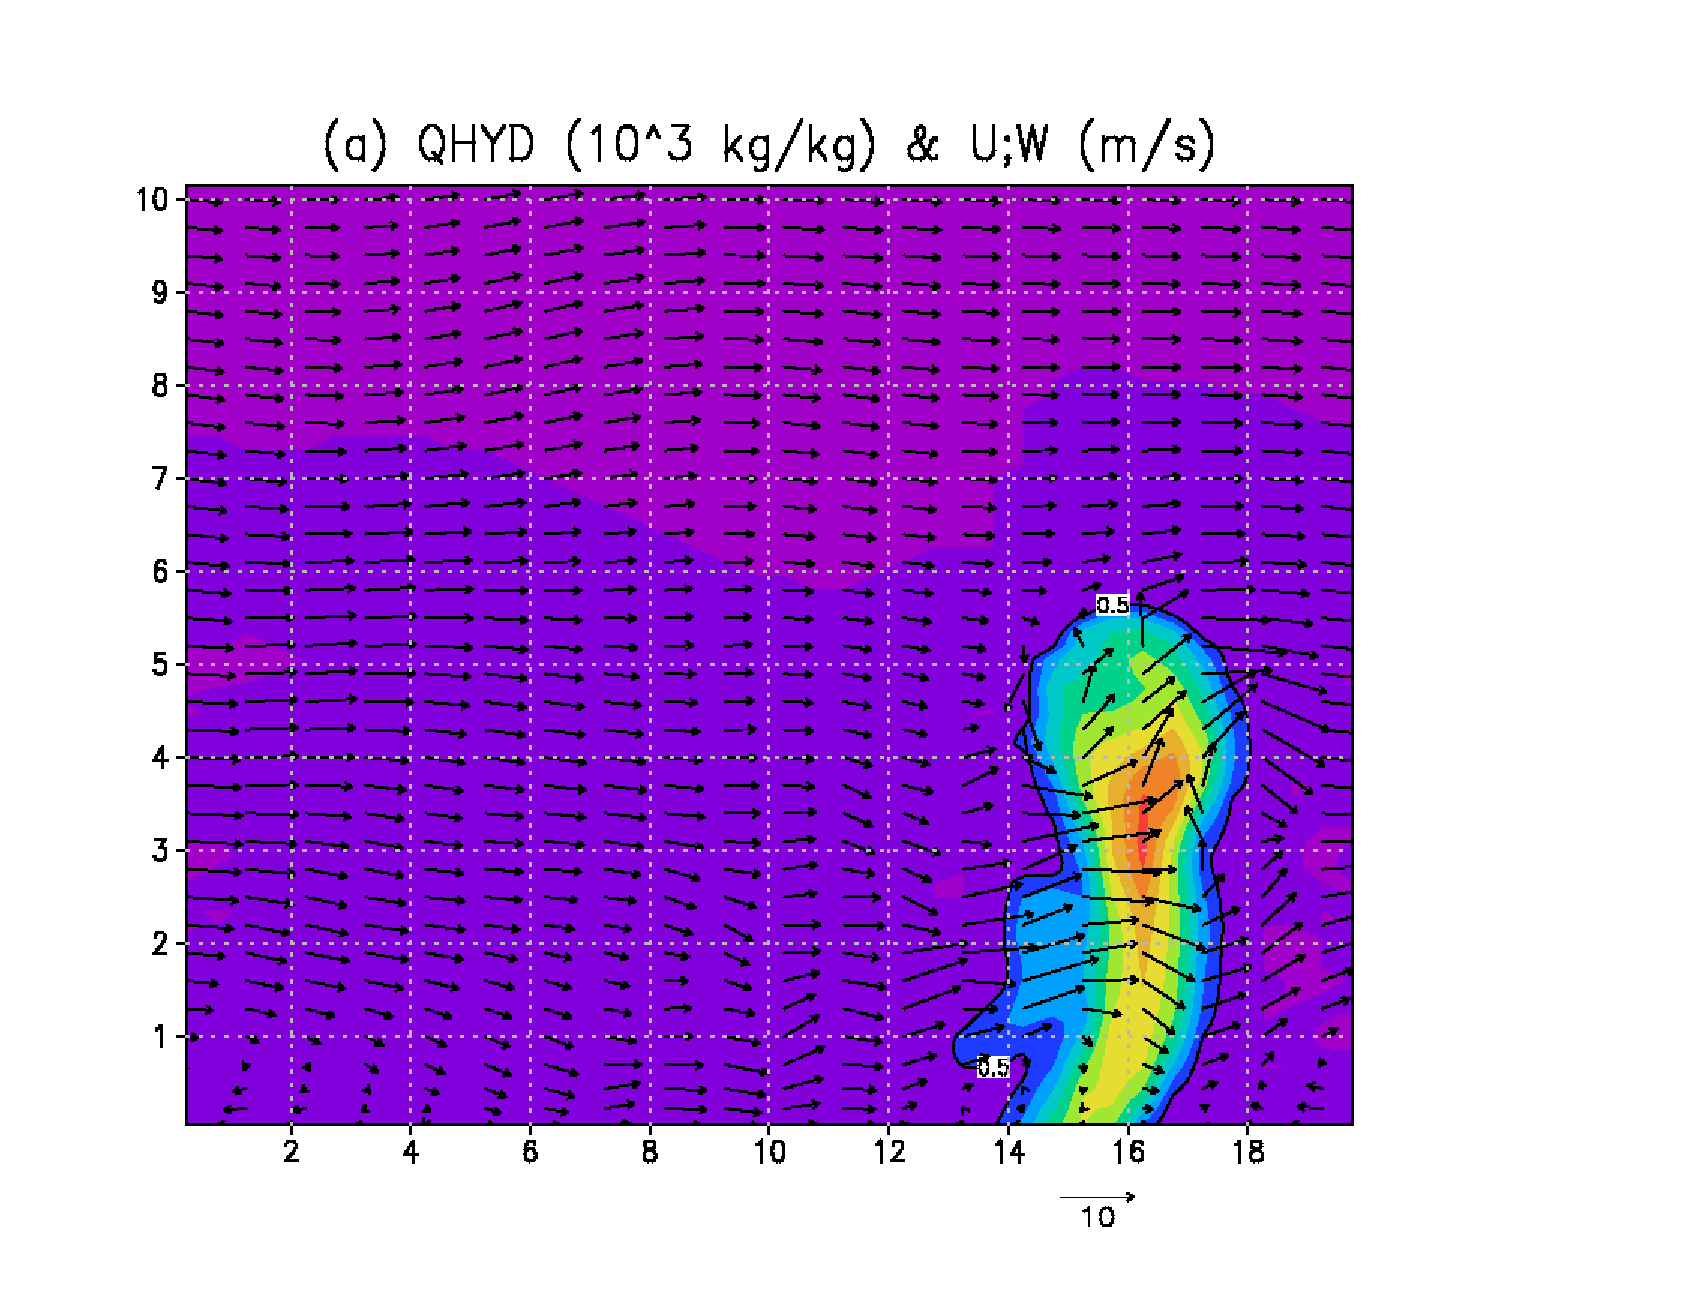
\includegraphics[width=0.7\hsize]{./figure/ideal_qhyd.eps}\\
  \includegraphics[width=0.7\hsize]{./figure/ideal_W.eps}\\
  \caption{The horizontal-vertical cross-section at Y=750m after t=1200 s (20 minutes later);
            The color indicates (a) the mass concentration of the hydrometeor and (b) vertical velocity. The vector indicates flow in both of figures.}
  \label{fig_ideal}
\end{center}
\end{figure}

To convert the result of the output into binary data for other variables,
add them to \nmitem{VNAME} in \namelist{VARI} in the configuration file \verb|net2g.conf|:
\editbox{
\verb|&VARI|\\
\verb| VNAME       = "U","W","QHYD"|\\
\verb|/|\\
}
To check the output variable in the history file, use \verb|ncdump| of {\netcdf}.
Refer to Section \ref{sec:net2g} for the detailed use of net2g. 


\section{Guideline for further study} \label{sec:ideal_exp_last}

In this chapter,
the method for the execution of \scalerm was explained by using a simple ideal experiment. We recommend studying methods of changing the model resolution, the calculation domain, and the number of MPI processes for further study.  With regard to the ideal experiment, several files of other configurations,  e.g., to increase resolution, the number of domains, and the physical scheme, are prepared in the directory ``sample'' under the same directory as was used in this experiment.  These configuration files are useful to change such configurations.  Moreover, various ideal experimental settings  have been prepared in the directory ``\verb|scale-rm/test/case|.'' For some ideal experiments,  it may be necessary to carry out the ``make'' command again in the same directory as in the configuration file  because some test cases need special source codes according to their experimental settings. The procedures for the generation of the initial conditions and those for simulation execution are the same as in the tutorial in this chapter.

It is important to study the method for the configuration of physical processes, such as cloud microphysics, radiation, and turbulence schemes. Methods to alter them in detail are described in Part \ref{part:basic_usel}.



%\chapter{理想大気実験}

\chapter{現実大気実験} \label{chap:tutorial_real}
%-------------------------------------------------------%
\section{概要} \label{sec:tutrial_real_intro}
%-------------------------------------------------------%
本章では、チュートリアルとして準備した現実大気実験の基本的な実行手順を習得する。
現実大気実験は、次の流れ(図\ref{fig:howto}) に従って実行する。
\begin{enumerate}
\item  入力データの準備 (基本各自で準備。チュートリアルでは \verb|tools/| で行う。)
\item  \texttt{pp}      : 地形データの作成
\item  \texttt{init}    : 初期値・境界値データの作成
\item  \texttt{run}     : シミュレーションの実行
\item  \texttt{net2g}   : 出力データの\netcdf から\grads 形式への変換(オプション)
\end{enumerate}

\begin{figure}[b]
\begin{center}
  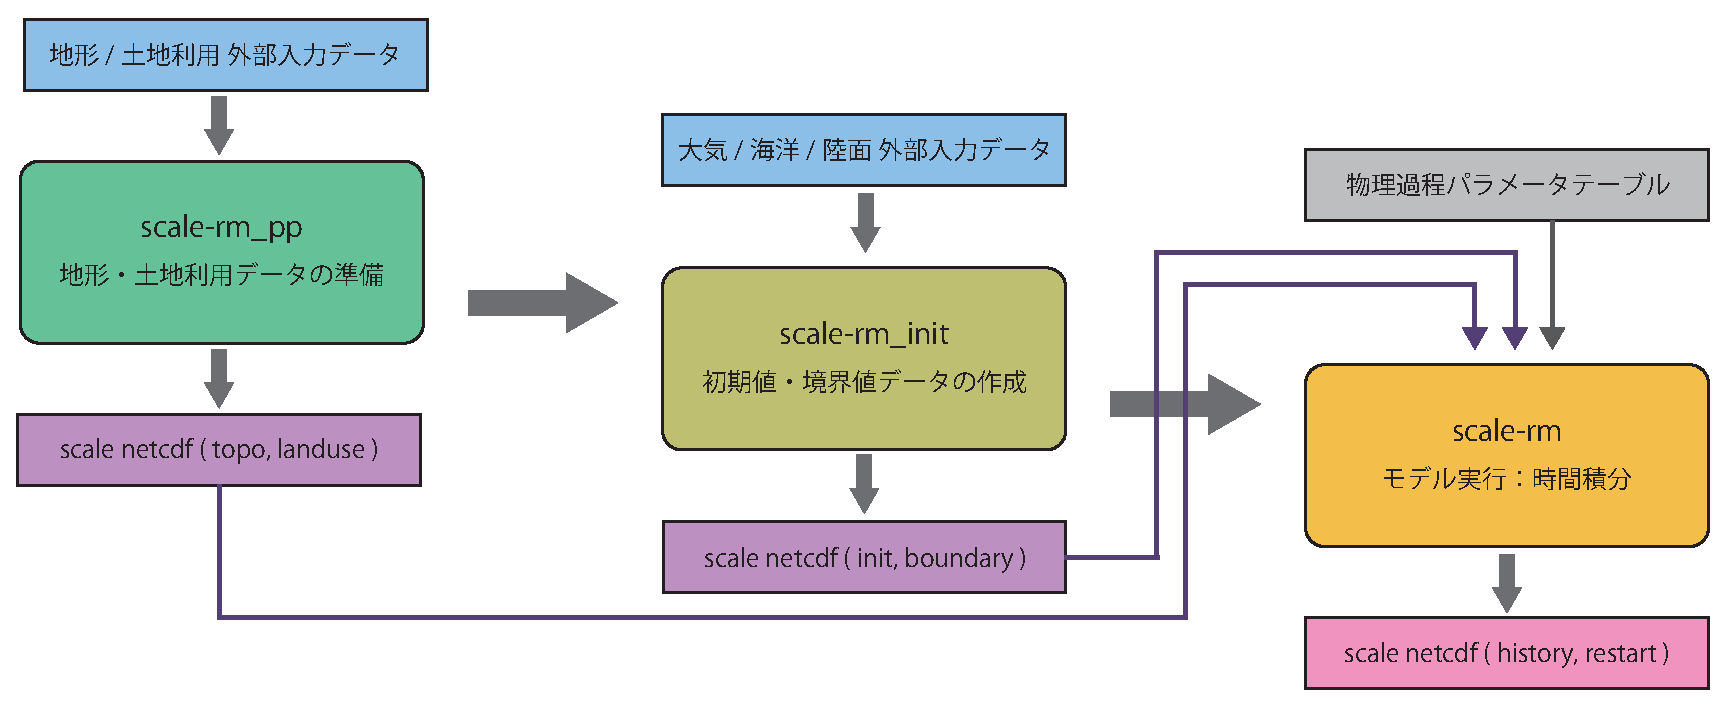
\includegraphics[width=0.9\hsize]{./figure/real_procedure.eps}\\
  \caption{\scalerm モデルの実行過程}
  \label{fig:howto}
\end{center}
\end{figure}


これ以降の説明では、\texttt{scale-{\version}/scale-rm/test/tutorial/}の絶対パスを
\verb|${Tutorial_DIR}|と示すこととする。


チュートリアルの現実大気実験の計算領域(ドメイン)の設定は表\ref{tab:grids}のようになっている。
図 \ref{fig:tutrial_real_domain}に対象領域を示す。
このチュートリアルは、\scalerm の使い方を学ぶことが目的であり、
短い時間で実行可能な設定にしている。
領域モデルの実験設定として必ずしも適切な設定を選択しているとは限らないので
ご留意頂きたい
(例えば、20kmの水平解像度で積雲パラメタリゼーションなし)。
%本章のチュートリアルを比較的短時間で実行するには、下記の条件を満たす計算機環境が推奨される。
%\begin{itemize}
%\item CPU: 2コア以上の演算コアを持つCPU(4コア以上を推奨)
%\item Memory容量: 4GB以上をプログラムに割当可能(8GB以上を搭載した計算機を推奨)
%\item HDD空き容量: 7GB以上の空き容量
%\end{itemize}


\begin{table}[h]
\begin{center}
  \caption{実験設定の概略}
  \label{tab:grids}
  \begin{tabularx}{150mm}{|l|X|} \hline
    \rowcolor[gray]{0.9} 項目 & 設定 \\ \hline
    MPIプロセス分割 (東西 x 南北) & 2 x 2 (合計4プロセス) \\ \hline
    水平格子数 (東西 x 南北) & 90格子点 x 90格子点 \\ \hline
    鉛直層数                 & 36層                  \\ \hline
    水平格子間隔             & dx = dy = 20km       \\ \hline
    積分期間 & 2007年7月14日 18UTC~15日00UTC (6時間積分) \\ \hline
    時間ステップ間隔 & 90 sec (240 steps) \\ \hline
  \end{tabularx}
\end{center}
\end{table}

\begin{figure}[tb]
\begin{center}
  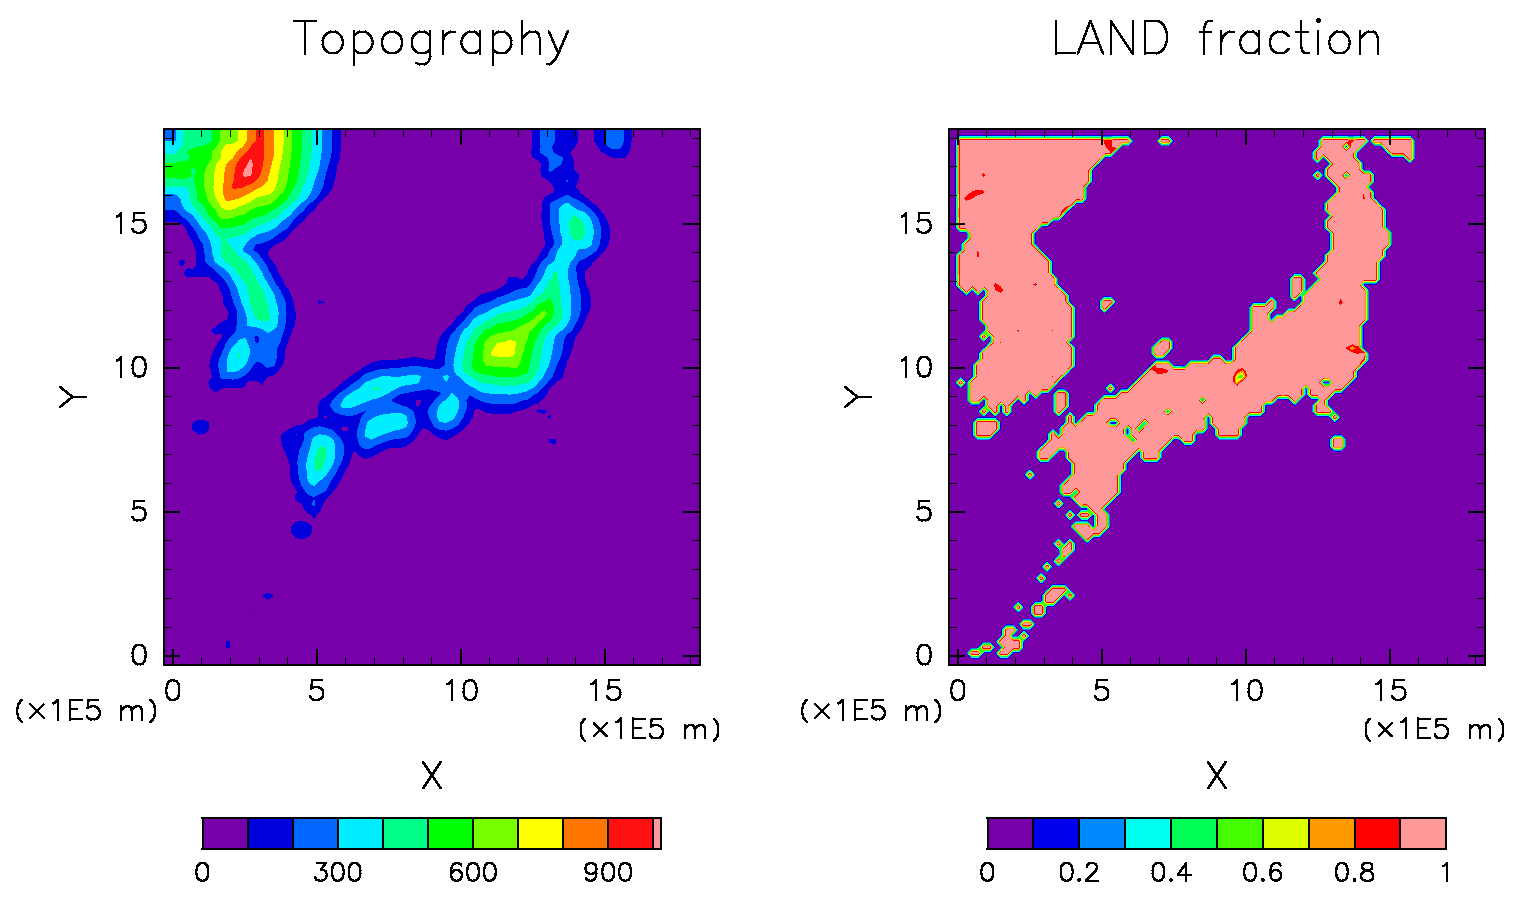
\includegraphics[width=1.0\hsize]{./figure/real_domain.eps}\\
  \caption{計算領域の地形と海陸分布.}
  \label{fig:tutrial_real_domain}
\end{center}
\end{figure}



%-------------------------------------------------------%
\section{入力データ(境界データ)の準備} \label{sec:tutrial_real_data}
%-------------------------------------------------------%

現実大気実験のシミュレーションを行う場合、\scalerm 本体に与える
境界値データが必要になる。境界値作成のための外部入力データとして
表\ref{tab:real_bnd}のデータが必要である。
{\color{blue}青字}は必須の変数、その他は任意である。

\begin{table}[h]
\begin{center}
  \caption{現実大気実験に必要な外部入力データ}
  \label{tab:real_bnd}
  \begin{tabularx}{150mm}{llX} \hline
    \multicolumn{3}{l}{\scalerm の地形と土地利用を作成するための元データ}\\ \hline
    & \multicolumn{2}{l}{\color{blue}{標高データ}}\\
    & \multicolumn{2}{l}{\color{blue}{土地利用区分データ}}\\ \hline
    \multicolumn{3}{l}{\scalerm の初期値境界値を作成するための外部入力データ(一般的にはGCMデータ)}\\ \hline
    &  \multicolumn{2}{l}{\color{blue}{親モデルの緯度・経度情報}}\\
    &  \multicolumn{2}{l}{(3次元大気データ)}\\
    & &  \multicolumn{1}{l}{\color{blue}{東西風速、南北風速、気温、比湿(相対湿度)、気圧、ジオポテンシャル高度}} \\
    &  \multicolumn{2}{l}{(2次元大気データ)}\\
    & & 海面更正気圧、地上気圧、10m東西風速、10m南北風速、2m気温、2m比湿(相対湿度) \\
    &  \multicolumn{2}{l}{(2次元陸面データ)}\\
    & &  \multicolumn{1}{l}{親モデルの海陸マップ}\\
    & &  \multicolumn{1}{l}{\color{blue}{地表面温度(Skin temp)}}\\
    & &  \multicolumn{1}{l}{{\color{blue}{親モデル土壌データの深さ情報、土壌温度}}、土壌水分(体積含水率 or 飽和度)}\\
    &  \multicolumn{2}{l}{(2次元海面データ)}\\
  & &  \multicolumn{1}{l}{\color{blue}{海面水温(Skin tempがある場合は省略可)}}\\ \hline
  \end{tabularx}
\end{center}
\end{table}

\subsubsection{標高データと土地利用区分データ}
標高データと土地利用区分データは実験設定に従って、
\scalerm のそれぞれの格子点における標高、海陸比率、湖比率、都市被覆率、植生比率、土地(植生)利用区分を
作成するために使用する。
ユーザーが全球の任意の地域を対象とした計算ができるよう、
フォーマット変換済みの
標高データ USGS(U.S. Geological Survey) のGTOPO30 と、
土地利用区分データ GLCCv2 を提供している。
%これらのデータベースを作成にするにあたり、施された前処理手順の詳細については、〇〇を参照すること(Todo)。

\begin{enumerate}
\item データのダウンロード\\
\scalerm 用の標高・土地利用区分のデータを\\
 \url{http://scale.aics.riken.jp/download/scale_database.tar.gz}\\
より入手し、任意のディレクトリに展開しておく。
展開したディレクトリには、標高データと土地利用区分データが格納されている。
\begin{alltt}
  $ tar -zxvf scale_database.tar.gz
  $ ls 
    scale_database/topo/    <- 標高データ
    scale_database/landuse/ <- 土地利用区分データ
\end{alltt}

\item パスの設定\\
現実大気実験の実験に必要なファイル一式の準備には、
makeを用いた「実験セット一式作成ツール」を用いる。
このツールを利用するためには、
標高・土地利用区分データの\verb|tar|ファイルの展開先ディレクトリを、
\verb|SCALE_DB| という環境変数に設定しておくことが必須である (以後、\verb|${SCALE_DB}|と表記)。
\begin{verbatim}
  $ export SCALE_DB="${path_to_directory_of_scale_database}/scale_database"
\end{verbatim}
ここで、\verb|${path_to_directory_of_scale_database}|は、
データベースがあるディレクトリである。
\end{enumerate}



\subsubsection{大気・陸面・海面水温データ}
初期値境界値データは4byteバイナリー(\grads 形式、以降``binary形式''と表記する)に変換すれば、
任意のデータを読み込むことが可能である。
基本的に、バイナリーデータはユーザー自身が用意する。
チュートリアルではNCEP FNL(Final) Operational Global Analysis data を使用する方法を示す。
あらかじめ\verb|wgrib|をインストールしておく\footnote{\url{http://www.cpc.ncep.noaa.gov/products/wesley/wgrib.html}}。

\begin{enumerate}
\item データのダウンロード\\
NCARのサイト
\url{http://rda.ucar.edu/datasets/ds083.2/}\\
から、2007年7月14日18時から一日分のgrib1フォーマットのデータ
\begin{alltt}
  fnl_20070714_18_00.grib1
  fnl_20070715_00_00.grib1
  fnl_20070815_06_00.grib1
  fnl_20070815_12_00.grib1
\end{alltt}
を\verb|${Tutorial_DIR}/real/tools/|の下にダウンロードする。

\item データフォーマットをgrib形式からbinary形式に変換\\
 \verb|${Tutorial_DIR}/real/tools/| にある\verb|convert_grib2grads_FNLgrib1.sh|を実行。

\begin{verbatim}
 $ cd ${Tutorial_DIR}/real/tools/
 $ sh convert_grib2grads_FNLgrib1.sh
\end{verbatim}
成功すれば、下記のファイルが作成される。
\begin{alltt}
 $ ls FNL_output/*/*
    FNL_output/200707/FNLatm_2007071418.grd
    FNL_output/200707/FNLatm_2007071500.grd
    FNL_output/200707/FNLatm_2007071506.grd
    FNL_output/200707/FNLatm_2007071512.grd
    FNL_output/200707/FNLland_2007071418.grd
    FNL_output/200707/FNLland_2007071500.grd
    FNL_output/200707/FNLland_2007071506.grd
    FNL_output/200707/FNLland_2007071512.grd
    FNL_output/200707/FNLsfc_2007071418.grd
    FNL_output/200707/FNLsfc_2007071500.grd
    FNL_output/200707/FNLsfc_2007071506.grd
    FNL_output/200707/FNLsfc_2007071512.grd
\end{alltt}
\end{enumerate}


%-------------------------------------------------------%
\section{Preparation for experiment set} \label{sec:tutrial_real_prep}
%-------------------------------------------------------%

In the real atmospheric experiment,
many execution procedures and a large number of files are needed in comparison with the ideal experiment.
In addition, it is necessary to maintain consistency between settings in the configuration file (\verb|***.conf|)
between pre-processing \verb|pp|, initial value making \verb|init|, and simulation execution \verb|run|.
The inconsistency between these settings and the lack of files in the preparation step may cause an abnormal model run.
To avoid such situations, the tool "the making tool for the complete settings of the experiment"
is prepared for the generation of a set of necessary files.
You first move to the following directory and prepare a series of files for the tutorial for the real atmospheric experiment using the next procedure:
\begin{verbatim}
 $ cd ${Tutorial_DIR}/real/
 $ ls
    Makefile : Makefile for generation of a set of necessary files.
    README   : README related to use of the script
    USER.sh  : Description of experimental setting.
    config/  : Each of configurations for generation of a set of files
               ( basically, unnecessary for users to be rewritten)
    sample/  : sample script of USERS.sh
    data/    : tools for the tutorial
    tools/   : tools for initial condition used in the tutorial 
               (basically, users do it themselves except for the tutorial case)
 $ make
 $ ls experiment/    : directories added by the above make command
    init/
    net2g/
    pp/
    run/
\end{verbatim}

According to the settings described in \verb|USER.sh|,
an experiment set is generated under the directory \verb|experiment| when the make command is executed.
Refer to Section \ref{sec:basic_makeconf} for a detailed explanation of "the making tool for the complete settings of the experiment."
%Further, in case of nesting, the available files are prepared for the directory \verb|sample|. Referred to them if needed.


%-------------------------------------------------------%
\section{Creating topographical data: pp} \label{sec:tutrial_real_pp}
%-------------------------------------------------------%

Move to the directory \verb|pp| and create topographical data for the experiment as follows:
\begin{verbatim}
 $ cd ${Tutorial_DIR}/real/experiment/pp/
 $ ls
    pp.d01.conf
    scale-rm_pp
\end{verbatim}
In the directory \verb|pp|, there exists configuration file \verb|pp.d01.conf|.
It is necessary to edit \verb|pp.d01.conf| according to the experiment settings,
such as the position of the domain and the number of grids.
Since \verb|pp.d01.conf| has already been edited for this tutorial, it can be used without any change.
The setting of this experiment is shown in Table \ref{tab:grids}.

In Namelists in \verb|pp.d01.conf|, the parameters related to the domain are configured in \namelist{PARAM_PRC},
\namelist{PARAM_INDEX}, and \namelist{PARAM_GRID}.
The domain is decomposed along each of the X and Y directions into two domains.
Thus, four MPI processes are used.
The number of grids per MPI process is \nmitem{IMAX = 45} and \nmitem{JMAX = 45}.
Thus, the total number of grids is 90 ($= 2 \times 45$) along the X and Y directions.
The grid spacings in each direction \nmitem{DX, DY} in \namelist{PARAM_GRID} is 20,000 m (20 km).
This means that the domain of calculation is an area of 1,800 km $\times$ 1,800 km because one side has length 90 $\times$ 20 km.
\editbox{
\verb|&PARAM_PRC| \\
\verb| PRC_NUM_X      = 2,| \\
\verb| PRC_NUM_Y      = 2,| \\
\verb| PRC_PERIODIC_X = .false.,| \\
\verb| PRC_PERIODIC_Y = .false.,| \\
\verb|/| \\
 \\
\verb|&PARAM_INDEX| \\
\verb| KMAX = 36,| \\
\verb| IMAX = 45,| \\
\verb| JMAX = 45,| \\
\verb|/| \\
 \\
\verb|&PARAM_GRID| \\
\verb| DX = 20000.0, |\\
\verb| DY = 20000.0, |\\
\verb| FZ(:) =    80.841,   248.821,   429.882,   625.045,   835.409,  1062.158,|\\
~~~~~~~~ \verb| 1306.565,  1570.008,  1853.969,  2160.047,  2489.963,  2845.575,|\\
~~~~~~~~ \verb| 3228.883,  3642.044,  4087.384,  4567.409,  5084.820,  5642.530,|\\
~~~~~~~~ \verb| 6243.676,  6891.642,  7590.074,  8342.904,  9154.367, 10029.028,|\\
~~~~~~~~ \verb|10971.815, 11988.030, 13083.390, 14264.060, 15536.685, 16908.430,|\\
~~~~~~~~ \verb|18387.010, 19980.750, 21698.615, 23550.275, 25546.155, 28113.205,|\\
\verb| BUFFER_DZ = 5000.0,   |\\
\verb| BUFFER_DX = 400000.0, |\\
\verb| BUFFER_DY = 400000.0, |\\
\verb|/| \\
}

\verb|scale-rm_pp| has a particular namelist of \namelist{PARAM_CONVERT}.
If \nmitem{CONVERT_TOPO=.true.}, the altitudes are processed.
If \nmitem{CONVERT_LANDUSE=.true.}, land-use classification data are processed.
\editbox{
\verb|&PARAM_CONVERT| \\
\verb|  CONVERT_TOPO    = .true.,| \\
\verb|  CONVERT_LANDUSE = .true.,| \\
\verb|/| \\
}

\nmitem{GTOPO30_IN_DIR} in \namelist{PARAM_CNVTOPO_GTOPO30}
and \nmitem{GLCCv2_IN_DIR} in\\ \namelist{PARAM_CNVLANDUSE_GLCCv2} specify the locations of altitude data and land-use classification data, respectively.
%They are the same as the path given by \verb|${SCALE_DB}|.
\editbox{
\verb|&PARAM_CNVTOPO_GTOPO30| \\
\verb| GTOPO30_IN_DIR       = "./topo/GTOPO30/Products",|\\
\verb| GTOPO30_IN_CATALOGUE = "GTOPO30_catalogue.txt",|\\
\verb|/|\\
\\
\verb|&PARAM_CNVLANDUSE_GLCCv2|\\
\verb| GLCCv2_IN_DIR        = "./landuse/GLCCv2/Products",|\\
\verb| GLCCv2_IN_CATALOGUE  = "GLCCv2_catalogue.txt",|\\
\verb| limit_urban_fraction = 0.3D0,|\\
\verb|/|\\
}

After preparation of the configure file,
execute \verb|scale-rm_pp| to create topographical data by the following command:
\begin{verbatim}
 $ mpirun  -n  4  ./scale-rm_pp  pp.d01.conf
\end{verbatim}
In the case of this tutorial, the number of MPI processes is four as in Table \ref{tab:grids}.
When the job is finished normally,
the following message is output at the end of the log file: \verb|pp_LOG_d01.pe000000|.
\msgbox{
 +++++ finalize MPI...\\
 +++++ MPI is peacefully finalized\\
}
Furthermore, the files \verb|topo_d01.pe######.nc| (file size of approximately 180 KB)  and\\
\verb|landuse_d01.pe######.nc| (file size of approximately 220 KB)  are generated,
dividing four files according to the MPI processes used.
\verb|######| represents the MPI process number.
The information concerning altitude, the ocean and land ratio, the lake ratio, urban covering and vegetation rates, and the classification of land use are stored at every grid point in these files.

\vspace{1cm}
\noindent {\Large\em OPTION} \hrulefill \\
When ``gpview'' is installed, you can confirm whether topographical data
has been correctly generated by the following command:
 \begin{verbatim}
   $ gpview topo_d01.pe00000*@TOPO --aspect=1 --nocont
   $ gpview landuse_d01.pe00000*@FRAC_LAND --aspect=1 --nocont
 \end{verbatim}
The same figure as Fig. \ref{fig:tutrial_real_domain} is generated
if the results are correct.


%-------------------------------------------------------%
\section{Creating the initial and boundary data: init} \label{sec:tutorial_real_init}
%-------------------------------------------------------%

Move to the directory \verb|init| and create the initial and boundary data for the \scalerm simulation as follows:
\begin{verbatim}
 $ cd ${Tutorial_DIR}/real/experiment/init
 $ ls
    init.d01.conf
    init.launch.conf
    param.bucket.conf
    scale-rm_init
\end{verbatim}

In the directory \verb|init|, there exists the configuration file \verb|init.d01.conf|.
The file \verb|init.launch.conf| also exists but is not used here.
It is necessary to edit the file \verb|init.d01.conf| according to such experimental settings as \verb|pp.d01.conf|. \verb|init.d01.conf| has been already edited for this tutorial experiment as shown in Table \ref{tab:grids}.  To create the initial and boundary data,  the topographical data generated in the previous section is used. This is set in \verb|init.d01.conf| to refer the relative path as follows:

\editbox{
\verb|&PARAM_TOPOGRAPHY| \\
\verb|   TOPOGRAPHY_IN_BASENAME = "../pp/topo_d01",| \\
\verb|/| \\
 \\
\verb|&PARAM_LANDUSE| \\
\verb|   LANDUSE_IN_BASENAME = "../pp/landuse_d01",| \\
\verb|/| \\
}
In particular,  the contents of \namelist{PARAM_MKINIT_REAL_ATMOS}, \namelist{PARAM_MKINIT_REAL_OCEAN} and \namelist{PARAM_MKINIT_REAL_LAND} are handled. It should be confirmed that the settings in \verb|init.d01.conf| are correct.
\editboxtwo{
\verb|&PARAM_MKINIT_REAL_ATMOS| & \\
\verb| NUMBER_OF_FILES      = 2,|                                   & {\small : number of files read } \\
\verb| FILETYPE_ORG         = "GrADS",|                             & {\small : choose from Table \ref{tab:inputdata_format}} \\
\multicolumn{2}{l}{\verb| BASENAME_ORG        = "namelist.grads_boundary.FNL.2005053112-2016051106",|}     \\
\verb| BASENAME_BOUNDARY    = "boundary_d01",|                      & {\small : output name of boundary data} \\
\verb| BOUNDARY_UPDATE_DT   = 21600.0,|                             & {\small : time interval of input data} \\
\verb| PARENT_MP_TYPE       = 3,|                                   & \\
\verb| USE_FILE_DENSITY     = .false.,|                             & {\small : use the atmospheric density in the parent model or not?} \\
\verb|/| \\
\\
\verb|&PARAM_MKINIT_REAL_OCEAN| & \\
\verb|   .........              |  & \\
\verb| INTRP_OCEAN_SFC_TEMP = "mask",|                              & {\small : how to treat the missing value of SST} \\
\verb| INTRP_OCEAN_TEMP     = "mask",|                              & {\small : how to treat the missing value of SST} \\
\verb|/| \\
\\
\verb|&PARAM_MKINIT_REAL_LAND| & \\
\verb|   ..........              | & \\
\verb| USE_FILE_LANDWATER   = .true.,|                              & {\small : use soil moisture data in the parent model or not?} \\
\verb| INTRP_LAND_TEMP      = "mask",|                              & {\small : how to treat the missing value of soil temperature} \\
\verb| INTRP_LAND_WATER     = "fill",|                              & {\small : how to treat the missing value of soil moisture} \\
\verb| INTRP_LAND_SFC_TEMP  = "fill",|                              & {\small : how to treat the missing value of surface temperate} \\
\verb|/| \\
}

The file format of the meteorological field data is specified in \nmitem{FILETYPE_ORG}. In this case, it is given as ``\grads'' to read data in \grads format. Refer to Section \ref{sec:adv_datainput} for the details of the input file.


Link the input data (FNL) that are converted into binary form in Section \ref{sec:tutorial_real_data} to the current working directory. A shell script for this appropriate linkage is prepared as \verb|"gradsinput-link_FNL.sh"| in the directory \verb|${Tutorial_DIR}/real/data|:
\begin{verbatim}
  $ cp ../../data/gradsinput-link_FNL.sh ./
  $ sh gradsinput-link_FNL.sh
\end{verbatim}
If the following linkages are found, it is successfully concluded.
\msgbox{
\verb|ATM_00000.grd -> ../tools/FNL_output/200707/FNL_ATM_2007071418.grd| \\
\verb|ATM_00001.grd -> ../tools/FNL_output/200707/FNL_ATM_2007071500.grd| \\
\verb|LND_00000.grd -> ../tools/FNL_output/200707/FNL_LND_2007071418.grd| \\
\verb|LND_00001.grd -> ../tools/FNL_output/200707/FNL_LND_2007071500.grd| \\
\verb|SFC_00000.grd -> ../tools/FNL_output/200707/FNL_SFC_2007071418.grd| \\
\verb|SFC_00001.grd -> ../tools/FNL_output/200707/FNL_SFC_2007071500.grd| \\
}

Then, link a namelist file to the directory \verb|init| to read the binary (\grads) data format in SCALE.
\begin{verbatim}
  $ ln -s ../../data/namelist.grads_boundary.FNL.2005053112-2016051106 ./
\end{verbatim}
After the above preparations, execute the \verb|scale-rm_init| using four MPI processes.
\begin{verbatim}
 $ mpirun -n 4 ./scale-rm_init init.d01.conf
\end{verbatim}

If the job finishes normally, the following files are generated:
\begin{verbatim}
 $ ls
    boundary_d01.pe000000.nc
    boundary_d01.pe000001.nc
    boundary_d01.pe000002.nc
    boundary_d01.pe000003.nc
    init_d01_20070714-180000.000.pe000000.nc
    init_d01_20070714-180000.000.pe000001.nc
    init_d01_20070714-180000.000.pe000002.nc
    init_d01_20070714-180000.000.pe000003.nc
    init_LOG_d01.pe000000
\end{verbatim}
The file \verb|init_LOG_d01.pe000000| is a log file.  The following message is output at the end of the file \verb|init_LOG_d01.pe000000|:
\msgbox{
 +++++ finalize MPI...\\
 +++++ MPI is peacefully finalized\\
}
The file sizes of the boundary and initial data, \verb|boundary_d01.pe######.nc| and \\
\verb|init_d01_20070714-180000.000.pe######.nc|, are approximately 18.9 MB and 12.6 MB, respectively,  where \verb|######| represents the MPI process number.

\subsection{Reducing memory usage in the high-performance computing}

In SCALE, the master process only reads input data, and broadcasts the data to each node.
This algorithm reduces file I/O and processes the input data fast.
On the other hand, the algorithm may cause insufficient memory error when reading large input data.
To avoid the error, you can choose the method that each node reads input data.

\editboxtwo{
\verb|&PARAM_MKINIT_REAL_ATMOS| & \\
\verb| SERIAL_PROC_READ = .false.,| & {\small : does the master process only read input data?} \\
\verb|/| \\
\\
}

The default setting is .true., which means that the master process only reads input data.
When setting .false., each node can access the input data and reduce memory usage.
However, because the algorithm places a load on file I/O,
the computational performance may deteriorate due to locking file access.

\vspace{1cm}
\noindent {\Large\em OPTION} \hrulefill \\
When ``gpview'' is installed,  one can confirm whether the initial and boundary data have been created correctly  by the following command:
\begin{verbatim}
 $ gpvect --scalar --slice z=1500 --nocont --aspect=1 --range=0.002:0.016 --int 0.001     \
          --xintv=10 --yintv=10 --unit_vect init_d01_20070714-180000.000.pe00*@QV         \
          init_d01_20070714-180000.000.pe00*@MOMX init_d01_20070714-180000.000.pe00*@MOMY \
          --title "QV, MOMX, MOMY"
\end{verbatim}
If the same figure as Fig. \ref{fig:init} is found, it is successfully concluded.

\begin{figure}[h]
\begin{center}
  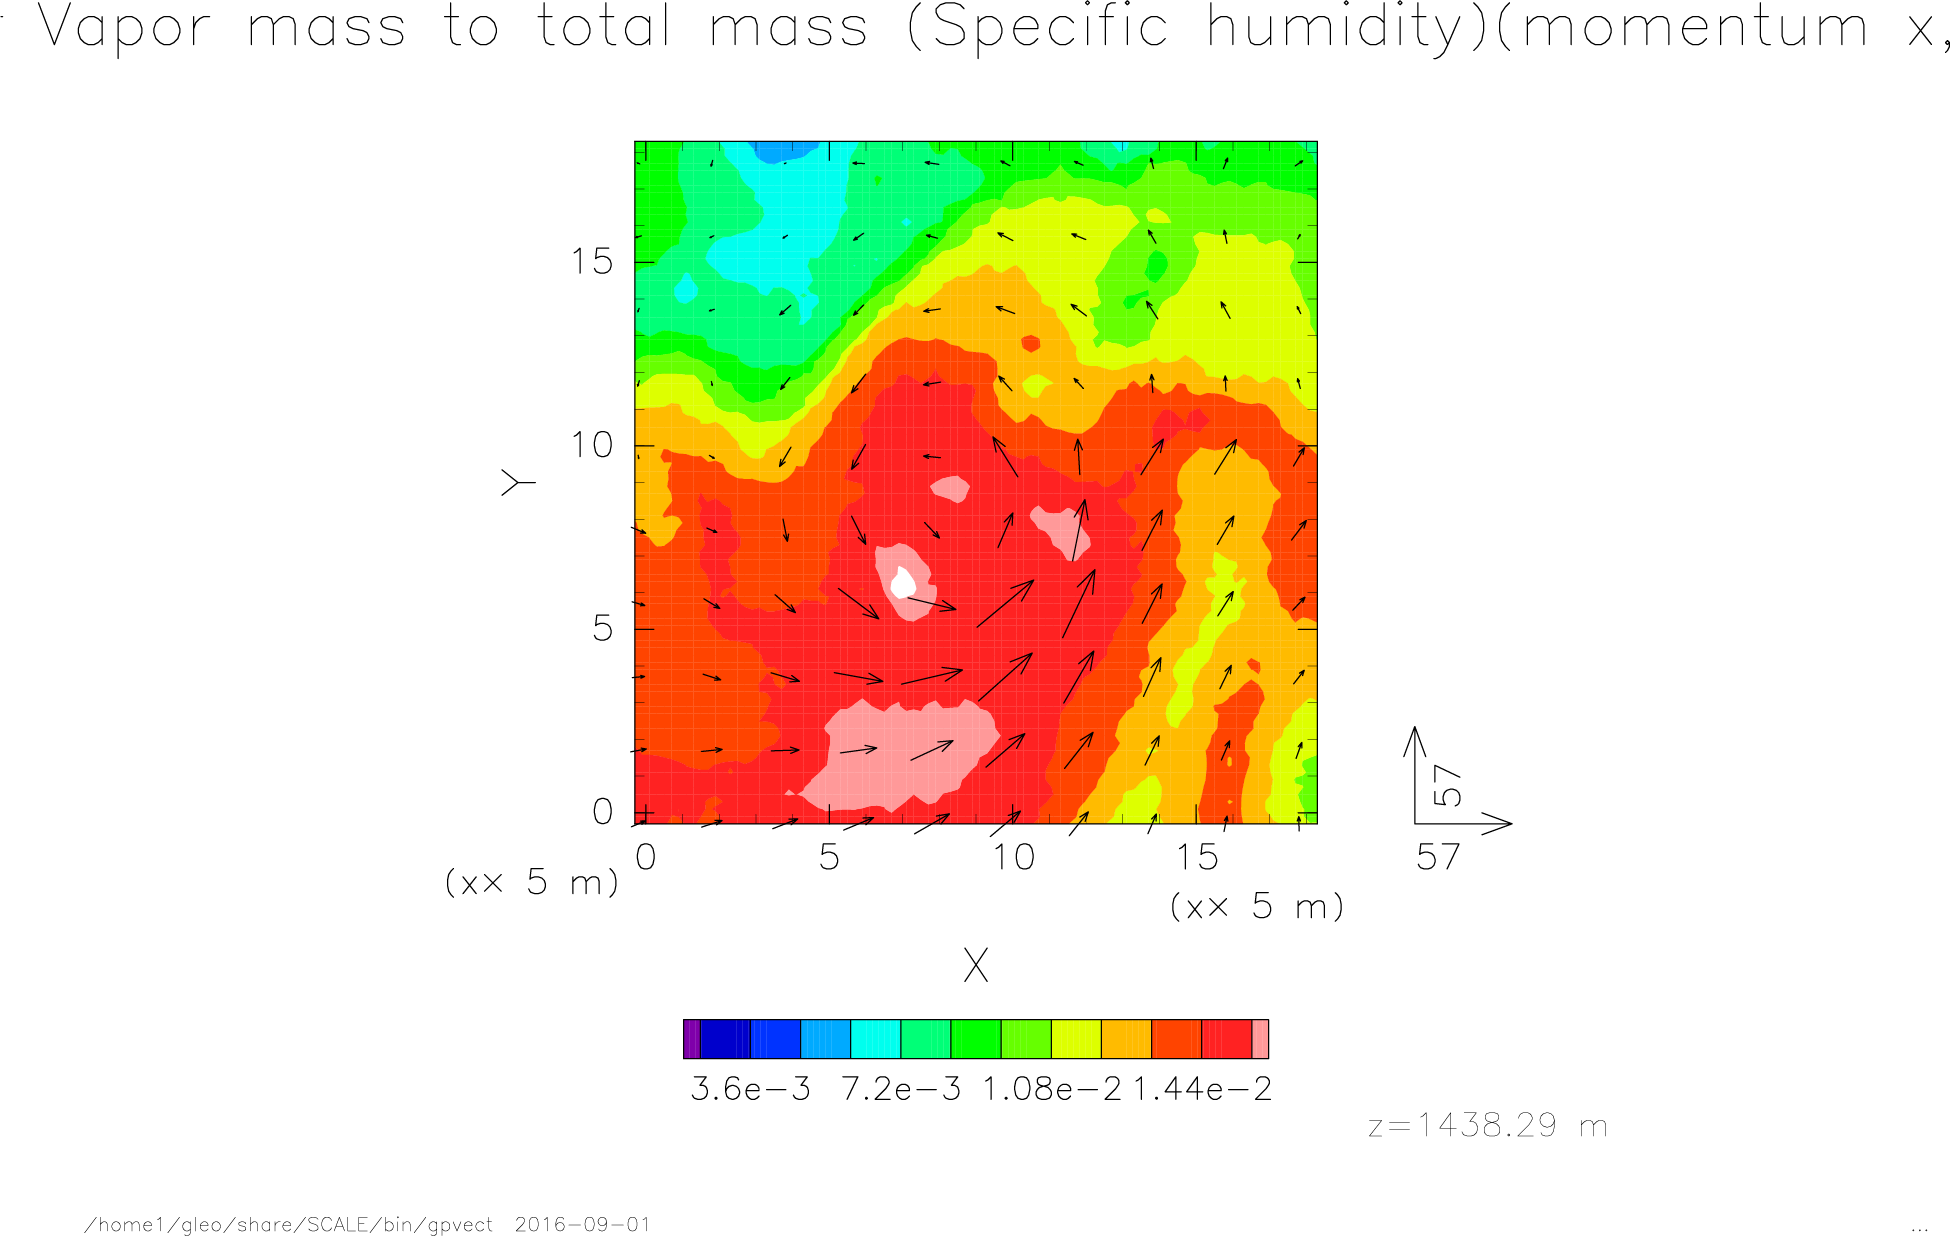
\includegraphics[width=0.6\hsize]{./../../figure/real_init_qv-momxy.pdf}\\
  \caption{Initial field at z=1500m for the tutorial experiment.
    The color indicates specific humidity and the vector horizontal momentum flux.}
  \label{fig:init}
\end{center}
\end{figure}

%-------------------------------------------------------%
\section{シミュレーションの実行:run} \label{sec:tutorial_real_run}
%-------------------------------------------------------%
\subsubsection{run.confの準備}
\verb|run|ディレクトリへ移動する。
\begin{verbatim}
 $ cd ${Tutorial_DIR}/real/experiment/run
\end{verbatim}
%
このディレクトリの中には、表\ref{tab:grids}に示すチュートリアル用の設定を施した設定ファイルが準備されている。
他に\verb|run.launch.conf|というファイルも存在するが、ここでは使用しない。

モデル本体の実行には、事前に作成した地形データや初期値/境界値データを使用する。
これらのファイルの指定は、\verb|run.d01.conf|における下記の部分で設定している。
\editbox{
\verb|&PARAM_TOPOGRAPHY| \\
\verb|   TOPOGRAPHY_IN_BASENAME = "../pp/topo_d01",| \\
\verb|/| \\
 \\
\verb|&PARAM_LANDUSE| \\
\verb|   LANDUSE_IN_BASENAME  = "../pp/landuse_d01",| \\
\verb|/| \\
 \\
\verb|&PARAM_RESTART| \\
\verb| RESTART_OUTPUT       = .true., |\\
\verb| RESTART_OUT_BASENAME = "restart_d01",|\\
\verb| RESTART_IN_BASENAME  = "../init/init_d01_20070714-180000.000",|\\
\verb|/| \\
 \\
\verb|&PARAM_ATMOS_BOUNDARY| \\
\verb| ATMOS_BOUNDARY_TYPE           = "REAL",                |\\
\verb| ATMOS_BOUNDARY_IN_BASENAME    = "../init/boundary_d01",|\\
\verb| ATMOS_BOUNDARY_USE_DENS       = .true.,     |\\
\verb| ATMOS_BOUNDARY_USE_QHYD       = .false.,    |\\
\verb| ATMOS_BOUNDARY_ALPHAFACT_DENS = 1.0,        |\\
\verb| ATMOS_BOUNDARY_LINEAR_H       = .false.,    |\\
\verb| ATMOS_BOUNDARY_EXP_H          = 2.0,        |\\
\verb|/| \\
}


\verb|run.d01.conf|の中で、時間積分に関する設定は\namelist{PARAM_TIME}で行う。
初期時刻は\nmitem{TIME_STARTDATE}にUTCで指定し、
チュートリアルでは2007年7月14日18時UTCに設定している。
積分時間は\nmitem{TIME_DURATION}で与える。
物理過程に対する時間ステップは、各物理スキームごとに設定できる。

\editboxtwo{
\verb|&PARAM_TIME| & \\
\verb| TIME_STARTDATE         = 2007, 7, 14, 18, 0, 0,| & ← 時間積分を開始する時刻 \\
\verb| TIME_STARTMS           = 0.D0,  | &\\
\verb| TIME_DURATION          = 6.0D0, | & : 積分期間 \\
\verb| TIME_DURATION_UNIT     = "HOUR",| & : \verb|TIME_DURATION|の単位\\
\verb| TIME_DT                = 90.0D0,| & : トレーサー移流計算の時間ステップ\\
\verb| TIME_DT_UNIT           = "SEC", | & : \verb|TIME_DT|の単位\\
\verb| TIME_DT_ATMOS_DYN      = 45.0D0,| & : トレーサー移流計算以外の力学過程の時間ステップ\\
\verb| TIME_DT_ATMOS_DYN_UNIT = "SEC", | & : \verb|TIME_DT_ATMOS_DYN|の単位\\
 \\
\verb|   ..... 略 .....              | & \\
 \\
\verb|/| &\\
}

計算結果の出力に関する設定は、\nmitem{PARAM_FILE_HISTORY}で行う。

\editboxtwo{
\verb|&PARAM_FILE_HISTORY| & \\
\verb|   FILE_HISTORY_DEFAULT_BASENAME  = "history_d01",| & : 出力するファイル名\\
\verb|   FILE_HISTORY_DEFAULT_TINTERVAL = 3600.D0,      | & : 出力時間間隔\\
\verb|   FILE_HISTORY_DEFAULT_TUNIT     = "SEC",        | & : 出力時間間隔の単位\\
\verb|   FILE_HISTORY_DEFAULT_TAVERAGE  = .false.,      | & \\
\verb|   FILE_HISTORY_DEFAULT_DATATYPE  = "REAL4",      | & \\
\verb|   FILE_HISTORY_DEFAULT_ZCOORD    = "model",      | & : 鉛直内挿は適用しない\\
\verb|   FILE_HISTORY_OUTPUT_STEP0      = .true.,       | & : 初期時刻(t=0)の値を出力するかどうか\\
\verb|/| \\
}

上記の設定に従って、下記の\nmitem{HISTOTRY_ITEM}に列挙した変数を出力する。
必要があれば、\nmitem{HISTOTRY_ITEM}においてオプション変数を加えることで、変数毎に出力間隔を変更できる。
また、瞬間値の代わりに平均値を出力することも可能である。
これらの詳細は、\ref{sec:output}を参照されたい。

\editboxtwo{
\verb|&HISTOTRY_ITEM name="MSLP" /|        & 海面更正気圧 \\
\verb|&HISTOTRY_ITEM name="PREC" /|        & 降水強度 (2次元) \\
\verb|&HISTOTRY_ITEM name="OLR"  /|        & 外向き赤外放射(2次元) \\
\verb|&HISTOTRY_ITEM name="U10m" /|        & 地表10mでの東西方向水平速度成分(2次元) \\
\verb|&HISTOTRY_ITEM name="V10m" /|        & 地表10mでの南北方向水平速度成分(2次元) \\
\verb|&HISTOTRY_ITEM name="U10" / |        & 地表10mでのX方向水平速度成分(2次元) \\
\verb|&HISTOTRY_ITEM name="V10" / |        & 地表10mでのY方向水平速度成分(2次元) \\
\verb|&HISTOTRY_ITEM name="T2"  / |        & 地表2mでの温度 (2次元) \\
\verb|&HISTOTRY_ITEM name="Q2"  / |        & 地表2mでの水蒸気比湿 (2次元) \\
\verb|&HISTOTRY_ITEM name="SFC_PRES"   /|   & 地表気圧 (2次元) \\
\verb|&HISTOTRY_ITEM name="SFC_TEMP"   /|   & バルクの地表面温度 (2次元) \\
\verb|&HISTOTRY_ITEM name="DENS" /|        & 密度 (3次元) \\
\verb|&HISTOTRY_ITEM name="QV"   /|        & 水蒸気比湿 (3次元) \\
\verb|&HISTOTRY_ITEM name="QHYD" /|        & 全凝結物の全質量に対する比 (3次元) \\
\verb|&HISTOTRY_ITEM name="PRES" /|        & 気圧 (3次元) \\
\verb|&HISTOTRY_ITEM name="Umet" /|        & 東西方向水平速度成分 (3次元) \\
\verb|&HISTOTRY_ITEM name="Vmet" /|        & 南北方向水平速度成分 (3次元) \\
\verb|&HISTOTRY_ITEM name="U"    /|        & X方向水平速度成分 (3次元) \\
\verb|&HISTOTRY_ITEM name="V"    /|        & Y方向水平速度成分 (3次元) \\
\verb|&HISTOTRY_ITEM name="T"    /|        & 温度 (3次元) \\
\verb|&HISTOTRY_ITEM name="W"    /|        & 鉛直方向速度成分 (3次元) \\
\verb|&HISTOTRY_ITEM name="Uabs" /|        & 風速 (3次元) \\
\verb|&HISTOTRY_ITEM name="PT"   /|        & 温位 (3次元) \\
\verb|&HISTOTRY_ITEM name="RH"   /|        & 相対湿度 (3次元) \\
}

力学過程や物理過程に対するスキームとして他のスキームを用いたい場合は、
力学過程に関しては\namelist{&PARAM_ATMOS_DYN}、
物理過程に関しては\namelist{PARAM_ATMOS,PARAM_OCEAN,PARAM_LAND,PARAM_URBAN}で設定できる。
詳細は、第\ref{sec:atmos_dyn_cartesC}節、\ref{sec:basic_usel_physics}節を参照されたい。

%
\subsubsection{シミュレーションの実行}

実行に必要なファイルは下記であり、あらかじめ用意されている。
\begin{alltt}
 $ ls
    MIPAS  PARAG.29  PARAPC.29  VARDATA.RM29  cira.nc
                                  : 放射スキーム用のパラメータファイル
    run.d01.conf      : 設定ファイル
    param.bucket.conf : 陸面スキーム用のパラメータファイル
    scale-rm          : \scalerm の実行バイナリ
    run.launch.conf   : ネスティング計算用のlaunchファイル
                       (チュートリアルでは使用しない)
\end{alltt}
%
準備が整ったら、4-MPI 並列により\scalerm を実行する。
\begin{verbatim}
  $ mpirun -n 4 ./scale-rm run.d01.conf >& log &
\end{verbatim}


実行が完了するまでには、ある程度時間を要する(推奨環境において10〜20分程度かかる)。
そのため、上記のように標準出力をファイルに書き出すようにして、
バックグラウンドで実行すると便利である。
計算は進みながら、途中経過のログは\verb|"LOG_d01.pe000000"|に出力される。
ジョブが正常に終了すると、\verb|"LOG_d01.pe000000"|の最後に
\msgbox{
 +++++ finalize MPI...\\
 +++++ MPI is peacefully finalized\\
}
と出力され、下記のファイルが作成される。
\begin{verbatim}
 $ ls
  history_d01.pe000000.nc
  history_d01.pe000001.nc
  history_d01.pe000002.nc
  history_d01.pe000003.nc
\end{verbatim}
各ファイルのサイズは約 34 MB である。
出力ファイル(\verb|history_d01.pe######.nc|)は、MPI プロセス数に応じて分割されている。
ここで、\verb|######|はMPIプロセス番号を表す。
これらのファイルには、\nmitem{HISTORY_ITEM}で指定した変数が出力されている。
出力ファイルの形式は、気候・予報(CF)メタデータ規約に準拠した NetCDF である。


%####################################################################################

\section{結果を描画する:net2g} \label{sec:quicklook}
%####################################################################################

ここでは、
プロセス毎に分割された{\netcdf}形式の出力ファイル(\verb|history.**.nc|
\footnote{gpviewがインストールされている場合、gpviewを使って作図することも出来る
gpviewならばhistoryデータを変換することなく直接作図することができるため、クイックチェックに適している。}
)を
{\grads}で読み込めるように1つのバイナリファイルにまとめる
\verb|netcdf2grads (略して、net2g)|の使い方と、変換した{\grads}バイナリデータを使って
結果の確認を行う。


\subsubsection{{\grads}バイナリに変換}
%-----------------------------------------------------------------------------------
プロセスごとに分割された{\netcdf}形式のhistoryファイルから
{\grads}バイナリ変換するには、\verb|net2g|を使用する。
詳細な使用方法は \ref{sec:net2g}節を参照頂くこととし、
ここでは最低限の手続きのみ説明する。\\

まず、\verb|net2g|ディレクトリへ移動する。
\begin{verbatim}
 $ cd ${Tutorial_DIR}/real/experiment/net2g
 $ ls
    net2g -> ../../../../../util/netcdf2grads_h/net2g
    net2g.2D.d01.conf
    net2g.3D.d01.conf
\end{verbatim}
中には設定ファイルとバイナリファイルがあり、
バイナリファイルは\ref{sec:source_net2g}節のコンパイルにより作成された
実行ファイルにリンクが貼られている。\\

ここでは例として、2次元変数のMSLP、PRECの変換と、
3次元変数のU、Vを850hPa、500hPa、200hPa面で抽出して変換する手順について説明する。
2次元変数のための設定ファイルは \verb|net2g.2D.d01.conf| に、
3次元変数のための設定ファイルは \verb|net2g.3D.d01.conf| に用意している。

\verb|netcdf2grads_h|実行時のプロセス数は、
計算実行時に使用したプロセス数の約数である必要がある。
ここでは、計算に用いた時と同じ4プロセスを使用する。
net2gでは2次元変数と3次元変数を同時に変換することはできないため、
別々に実行する。
\begin{verbatim}
 $ mpirun -n 4 ./net2g net2g.2D.d01.conf
 $ mpirun -n 4 ./net2g net2g.3D.d01.conf
\end{verbatim}
エラーメッセージがなく、下記のメッセージだけが標準出力へ表示されていれば正常に変換完了である。\\

\noindent {\gt
\fbox{
\begin{tabularx}{150mm}{l}
\verb|+++ MPI COMM: Corrective Finalize| \\
\end{tabularx}
}}\\

成功すれば、下記のファイルが作成される。
\verb|**.ctl|は {\scalerm} のXY格子座標のctlファイル、
\verb|**lccr.ctl|は緯度経度座標で作図するためのctlファイルである。

\begin{verbatim}
  MSLP_d01z-2d.ctl
  MSLP_d01z-2d.grd
  MSLP_d01z-2d_lccr.ctl
  PREC_d01z-2d.ctl
  PREC_d01z-2d.grd
  PREC_d01z-2d_lccr.ctl
  PRES_d01z-3d.ctl
  PRES_d01z-3d.grd
  PRES_d01z-3d_lccr.ctl
  U_d01z-3d.ctl
  U_d01z-3d.grd
  U_d01z-3d_lccr.ctl
  V_d01z-3d.ctl
  V_d01z-3d.grd
  V_d01z-3d_lccr.ctl
\end{verbatim}




\subsubsection{計算結果の確認}
%-----------------------------------------------------------------------------------

%\verb|${Tutorial_DIR}/real/data|ディレクトリに用意してあるので、
%サンプルとして利用してほしい。\footnote{今後、緯度経度座標で描画するためのctlファイルを出力できるようにする予定。}
%\begin{verbatim}
% $ cp ../../data/*_lcc.ctl ./
% $ ls
%    MSLP_d01z-2d_lcc.ctl
%    PREC_d01z-2d_lcc.ctl
%    U_d01z-3d_lcc.ctl
%    V_d01z-3d_lcc.ctl
%\end{verbatim}

計算結果確認用の図を作成するための\grads スクリプト\verb|checkfig_real.gs|を使って作図する。
\begin{verbatim}
 $ cp ../../data/checkfig_real.gs ./
 $ grads -blc checkfig_real.gs
\end{verbatim}
成功すると、下記の図が作成される。
なお、\grads のバージョンによって文法が異なるので、Warningが出る場合は、適宜変更する。
\begin{verbatim}
  real_mslp.png
  real_prec.png
  real_wind.png
\end{verbatim}
計算と変換が成功していれば、下記と同じ図が描画される。

\proofcomment{(足立)最後のチェックで図の入れ替え!!!}

\begin{figure}[h]
\begin{center}
  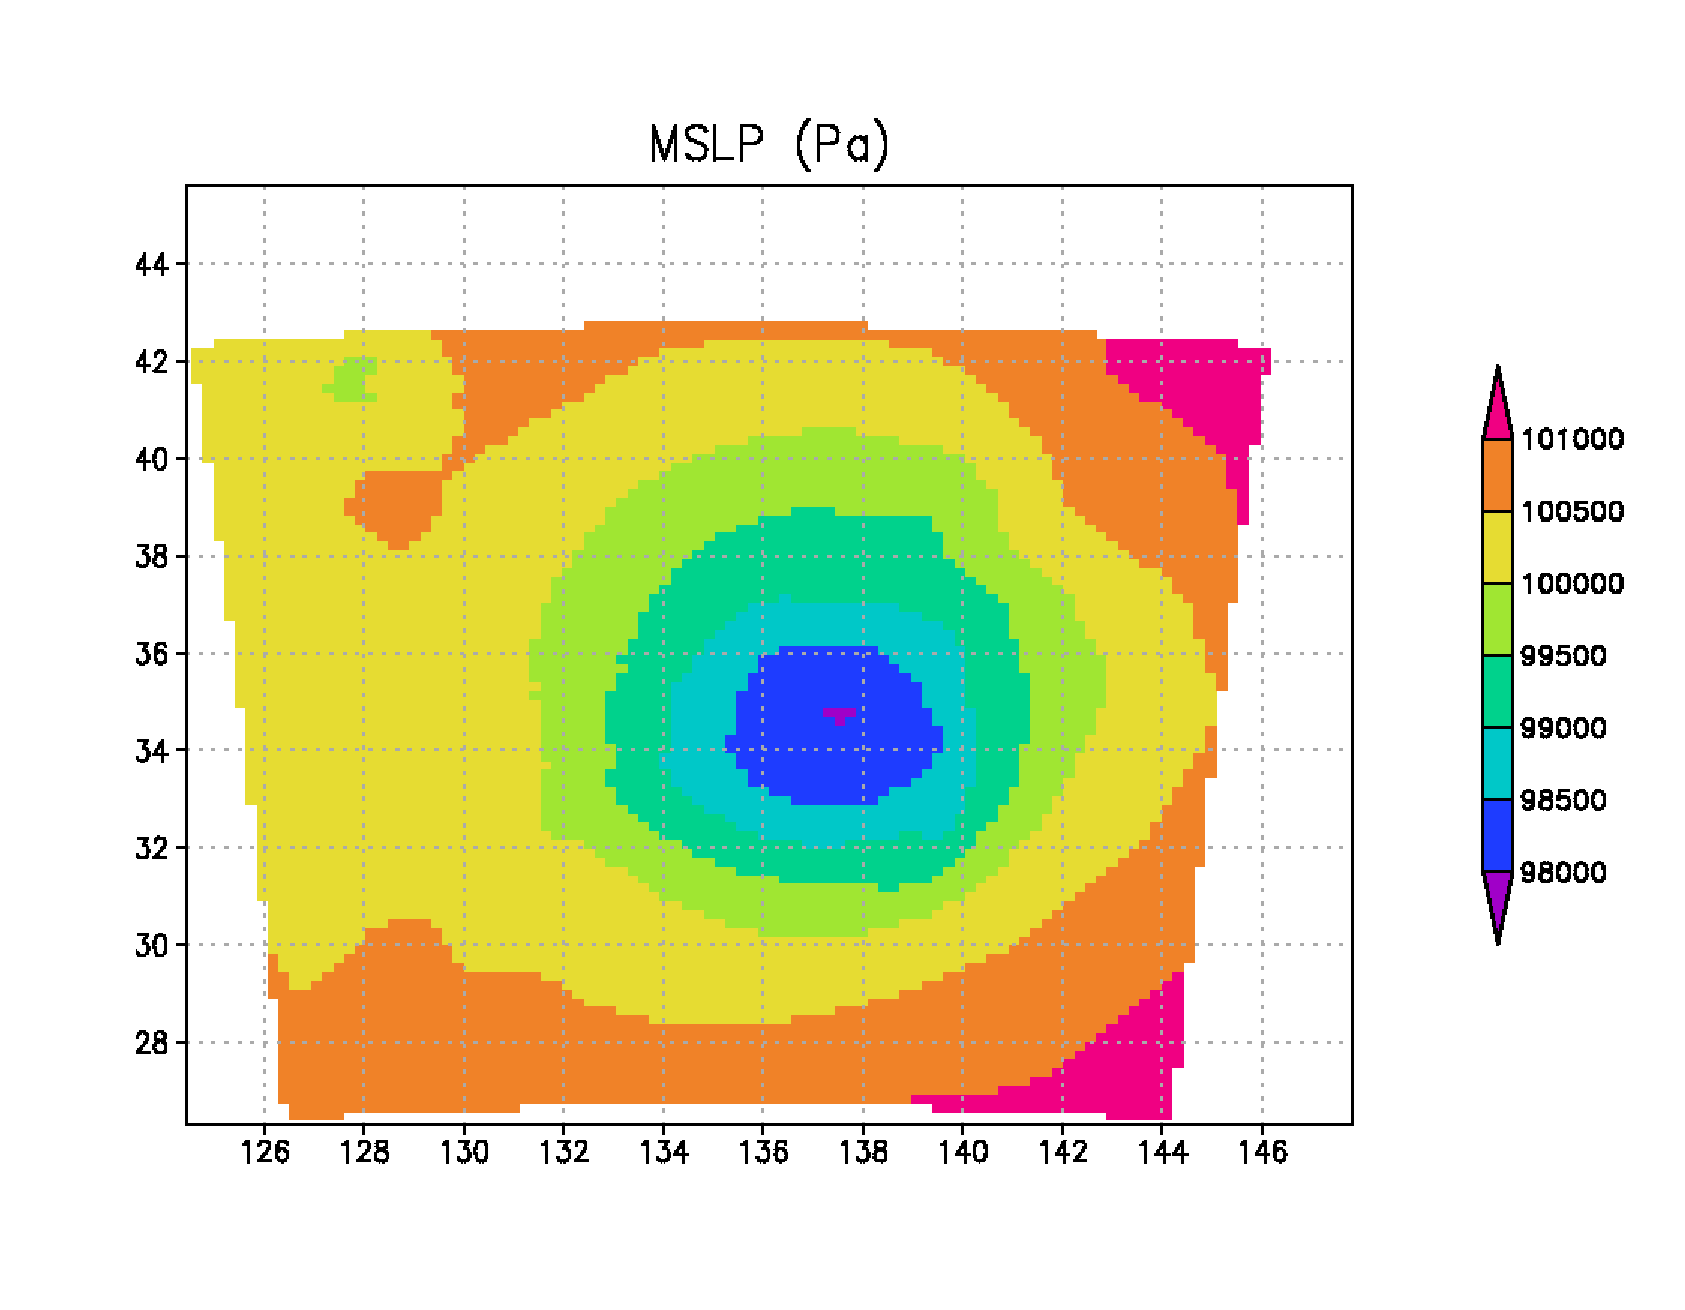
\includegraphics[width=0.55\hsize]{./figure/real_mslp.eps}\\
  \caption{計算開始から6時間後の海面更正気圧}
  \label{fig:real_mslp}
\end{center}
\begin{center}
  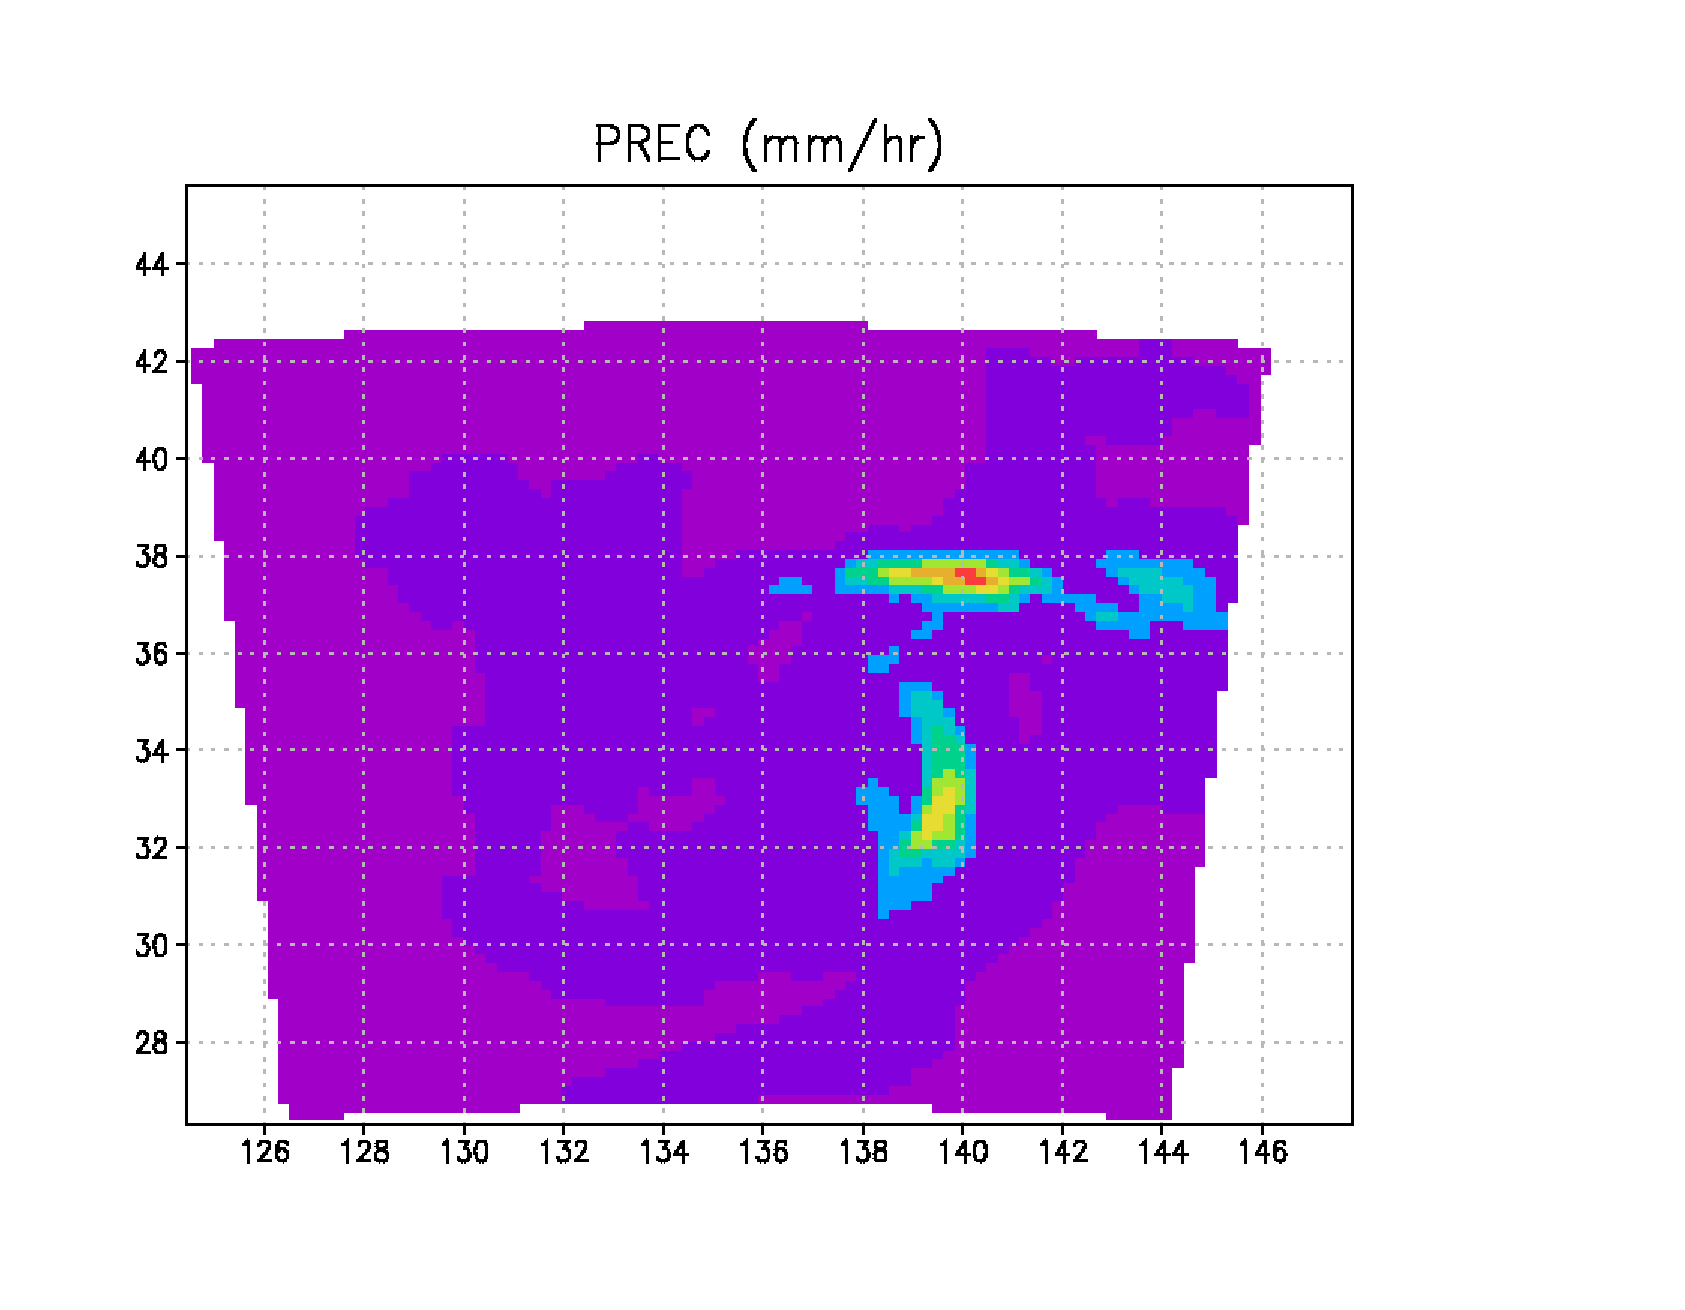
\includegraphics[width=0.55\hsize]{./figure/real_prec.eps}\\
  \caption{計算開始から6時間後の降水フラックス}
  \label{fig:real_prec}
\end{center}
\begin{center}
  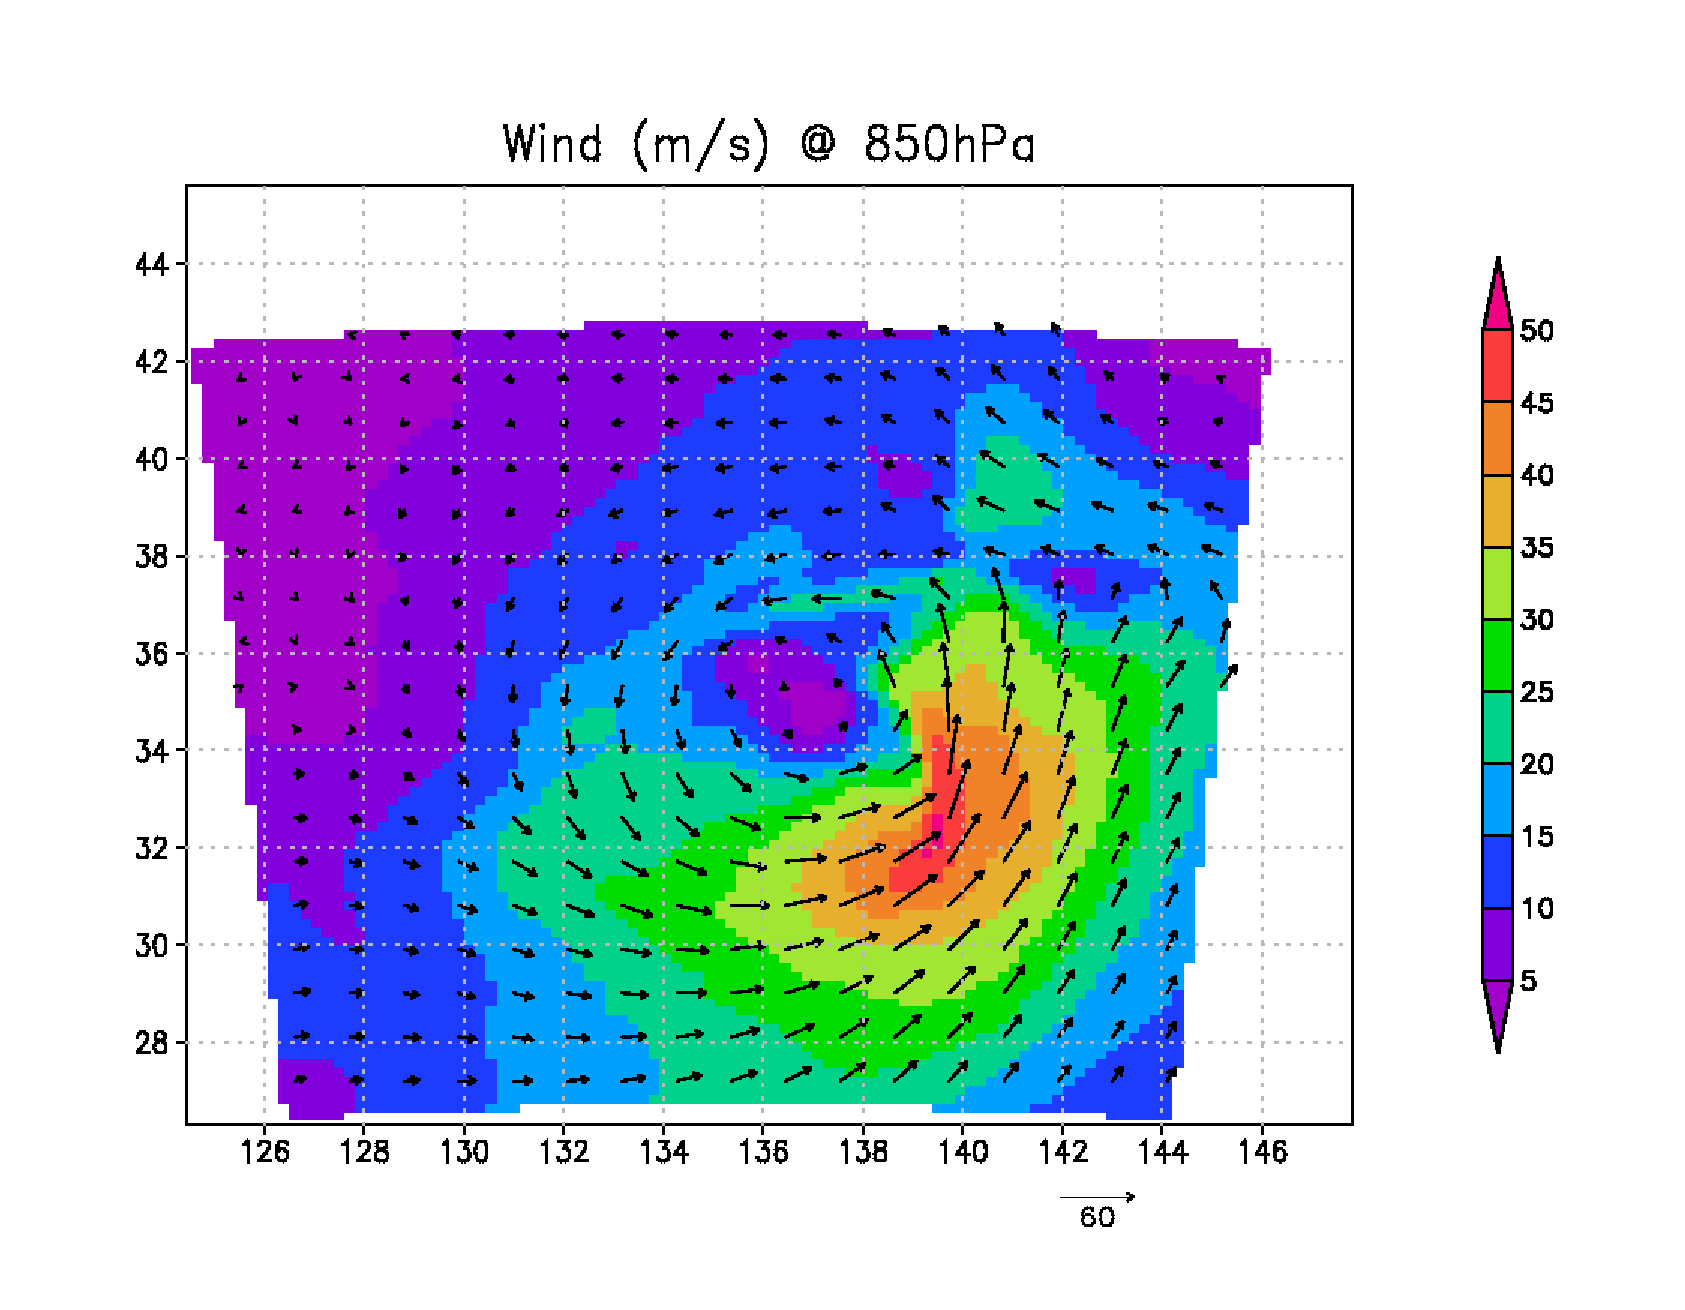
\includegraphics[width=0.55\hsize]{./figure/real_wind.eps}\\
  \caption{計算開始から6時間後の500hPaの風速と風ベクトル}
  \label{fig:real_wind}
\end{center}
\end{figure}



%\part{Tutorial for \scalegm}
% \chapter{Operation check and basic usage}
% %###############################################################################

This document is an additional volume of ``SCALE USERS GUIDE''.
This document includes a description of how to use SCALE-Global Model(GM) and a tutrial based on DCMIP2016.
The SCALE-GM is global atmospheric model constructed by using SCALE library.
The overview of SCALE library is described in Chapter 1 of ``SCALE USERS GUIDE''.

In current version, SCALE-GM supports ideal simulations for the dynamical core test.
SCALE-GM is originated from a dynamical core, developed for Nonhydrostatic ICosahedral Atmospheric Model (NICAM).
%The development of NICAM with full physics has been co-developed mainly by
%the Japan Agency for Marine-Earth Science and Technology (JAMSTEC), Atmosphere
%and Ocean Research Institute (AORI) at The University of Tokyo, and RIKEN / Advanced
%Institute for Computational Science (AICS).
A reference paper for NICAM is
Tomita and Satoh (2004), Satoh et al. (2008).
%See also NICAM.jp (\url{http://nicam.jp/}).

\section{Terms of SCALE-GM}
%-------------------------------------------------------------------------------

 \begin{itemize}
   \item g-level (grid level): number of subdivision times of the grid from the original icosahedron.
         the number starts from 1, we recommend to use the number larger than 4.
   \item r-level (region level): number of subdivision times of the region(tile)
         from the original icosahedron. When r-level = 0, we have ten regions(tiles).
         At that time, the number of available maximum MPI processes is ten.
 \end{itemize}


\section{Note}
%-------------------------------------------------------------------------------
 \begin{itemize}
   \item Explanations are based on bash environment below.
         In the tcsh environment, use "setenv" command instead of "export".
         (e.g. \verb|> setenv SCALE_SYS "Linux64-gnu-ompi"|)
   \item A symbol of "\verb|>|" means execution of commands in the console.
   \item Gothic means output from standard output.
%   \item \$\{TOP\}   means \verb|scale/scale-gm|
%   \item \$\{ROOT\}  means \verb|scale|
 \end{itemize}


% %\textcolor{red}{[英語版対応、要推敲-----ここから]}
%%%%%%%%%%%%%%%%%%%%%%%%%%%%%%%%%%%%%%%%%%
%%%% IV.1.1 Preparation of databases %%%%
%%%%%%%%%%%%%%%%%%%%%%%%%%%%%%%%%%%%%%%%%%
\section{Preparataion of databases: Horizontal grid}
%-------------------------------------------------------------------------------

To run the scale-gm, you need to prepare horizontal grid databases.
The database for g-level=5, r-level=0, and 10 MPI processes
is included in the tarball, as an example.
However, if you use a different set of settings, you need to prepare databases
either by donwloading prepared databases or by creating them yourself.


%%%%%%%%%%%%%%%%%%%%%%%%%%%%%%%%%%%%%%%%%%
%%%% IV.1.1.1 Use preprepared databases %%%%
%%%%%%%%%%%%%%%%%%%%%%%%%%%%%%%%%%%%%%%%%%
\subsection{Use preprepared databases}
The databases for some of the typical settings\footnote{At the time of
  writing, the following files are available:
  \begin{itemize}
    \item scale-gm\_database\_gl04rl00pe10.tar.gz
    \item scale-gm\_database\_gl05rl01pe40.tar.gz
    \item scale-gm\_database\_gl06rl01pe40.tar.gz
    \item scale-gm\_database\_gl07rl02pe160.tar.gz
\end{itemize}} can be downloaded from \noindent \url{https://scale.riken.jp/ja/download/}

Suppose you use g-level=6, r-level=1, 40 MPI processes,
Download and untar scale-gm\_database\_gl06rl01pe40.tar.gz,
 then you have 40 boundary (horizontal grid database)
files and 41 llmap (LatLon
grid conversion table) files.
\begin{verbatim}
  $ tar -zxvf scale-gm_database_gl06rl01pe40.tar.gz
\end{verbatim}

\noindent Then you need to move each database to appropriate directories.

\noindent First the boundary files are moved to a new directory under
\texttt{scale-{\version}/scale-gm/test/data/grid/boundary}
Suppose we are in the untared directory, use the following commands
\\

\verb|  $ mkdir scale-|{\version}\verb|/scale-gm/test/data/grid/boundary/gl06rl01pe40|

\verb|  $ mv boundary_GL06RL01.* scale-|{\version}\verb|/scale-gm/test/data/grid/boundary/gl06rl01pe40/|
\\

\noindent The llmap files are moved to a new directory under
\texttt{scale-{\version}/scale-gm/test/data/grid/llmap}

\verb|  $ mkdir -p scale-|{\version}\verb|/scale-gm/test/data/grid/llmap/gl06/rl01|

\verb|  $ mv llmap.* scale-|{\version}\verb|/scale-gm/test/data/grid/boundary/gl06/rl01/| \\


%%%%%%%%%%%%%%%%%%%%%%%%%%%%%%%%%%%%%%%%%%
%%%% Creation of new databases %%%%%%%%%
%%%%%%%%%%%%%%%%%%%%%%%%%%%%%%%%%%%%%%%%%%
\subsection{Create new databases}
\textcolor{red}{[要検討: ここで言及するのがいいのか、後(例えば3章)の方がいいのか]}

Creating horizontal grid databases consist of the three steps: Creation of
\begin{enumerate}
  \item Process managing database
  \item Raw grid database
  \item Horizontal grid database
\end{enumerate}

%\renewcommand{\labelenumi}{(\roman{enumi})}
%%%% Creation of horizontal grid databases %%%%%%%%%
\subsubsection{Creation of process managing database}

If the target directory does not exist, make it \\

\verb|  $ mkdir scale-|{\version}\verb|/scale-gm/test/framework/mkmnginfo/rl01pe40| \\

\verb|  $ cd scale-|{\version}\verb|/scale-gm/test/framework/mkmnginfo/rl01pe40| \\

Then copy Makefile and mkmnginfo.cnf from an exisiting sample directory
\begin{verbatim}
  $ cp ../rl00pe10/Makefile .
  $ cp ../rl00pe10/mkmnginfo.cnf .
\end{verbatim}

Edit the Makefile
\editboxtwo{
\verb|# parameters for run| & \\
\verb|    glevel      = none| &\\
\verb|    rlevel      = 1|               &{\verb|<-- rlevel|} \\
\verb|    nmpi        = 40|                    &{\verb|<-- number of processors|} \\
\verb|    zlayer      = none| &\\
\verb|    vgrid       = none| & \\
}

Edit the mkmnginfo.cnf
\editboxtwo{
\verb|&mkmnginfo_cnf| & \\
\verb|  rlevel       = 1,|                   &   {\verb|<-- rlevel |}\\
\verb|  prc_num      = 40,|                  &   {\verb|<-- number of processors|}\\
\verb|  output_fname = "../../../data/mnginfo/rl01-prc40.info",|   &   {\verb|<-- output filename|}\\
\verb|/|&\\
}

\vspace{-4mm}
\begin{verbatim}
  $ make jobshell
  $ make run
\end{verbatim}
If it is successfuly completed, the outpuf file specified as {\verb|output_fname|} is created.


% (ii) Creation of raw grid database %
\subsubsection{Creation of raw grid database}
If the target directry does not exist, make it \\

\verb|  $ mkdir scale-|{\version}\verb|/scale-gm/test/framework/mkrawgrid/gl05rl01pe40| \\

\verb|  $ cd scale-|{\version}\verb|/scale-gm/test/framework/mkrawgrid/gl05rl01pe40|

Copy Makefile and mkrawgrid.cnf from an exisiting sample directory \\

\begin{verbatim}
  $ cp ../../rl00pe10/Makefile .
  $ cp ../../rl00pe10/mkrawgrid.cnf .
\end{verbatim}

Edit the Makefile
\editboxtwo{
\verb|# parameters for run |&\\
\verb|glevel      = 5|             & {\verb|<-- glevel|} \\
\verb|rlevel      = 1|             & {\verb|<-- rlevel|} \\
\verb|nmpi        = 40|            & {\verb|<-- number of processors|} \\
\verb|zlayer      = none |& \\
\verb|vgrid       = none |& \\
}

Edit the mkrawgrid.cnf
\editboxtwo{
\verb|&ADMPARAM |&\\
\verb|  glevel      = 5,|                &{\verb|<-- glevel|}\\
\verb|  rlevel      = 1,|                &{\verb|<-- rlevel|}\\
\verb|  vlayer      = 1,|                &{\verb|<-- vertical layer?|}\\
\verb|  rgnmngfname = "rl01-prc40.info",|    &{\verb|<-- input filename|}\\
\verb|/|&\\

\verb|&PARAM_MKGRD|& \\
\verb|  MKGRD_DOSPRING     = .true.,|       &{\verb|<-- use spring grid or not|}\\
\verb|  MKGRD_OUT_BASENAME = "rawgrid_GL05RL01",| &{\verb|<-- output filename|}\\
\verb|  MKGRD_spring_beta  = 1.15D0,|         &{\verb|<-- strength of the spring|}\\
\verb|/|&\\
}


\vspace{-4mm}
\begin{verbatim}
  $ make jobshell
  $ make run
\end{verbatim}
I it is successfully completed, the output files ({\verb|rawgrid_GL05RL01.pe0000[00-39]|}) are created in
the same directory.



% Creation of horizontal grid database %
\subsubsection{Creation of horizontal grid database}
If the target directory does not exist, make it \\

\verb|  $ mkdir scale-|{\version}\verb|/scale-gm/test/framework/mkhgrid/gl05rl01pe20| \\

\verb|  $ cd scale-|{\version}\verb|/scale-gm/test/framework/mkhgrid/gl05rl01pe20| \\
Copy Makefile and mkhgrid.cnf from an exisiting sample directory
\begin{verbatim}
  $ cp ../../rl00pe10/Makefile .
  $ cp ../../rl00pe10/mkhgrid.cnf .
\end{verbatim}

Edit the Makefile
\editboxtwo{
\verb|# parameters for run |&\\
\verb|  glevel      = 5|    &{\verb|<-- glevel|}\\
\verb|  rlevel      = 1|    &{\verb|<-- rlevel|}\\
\verb|  nmpi        = 40|   &{\verb|<-- number of processors|}\\
\verb|  zlayer      = none |& \\
\verb|  vgrid       = none |& \\
}

Edit the mkhgrid.cnf
\editboxtwo{
\verb|&ADMPARAM | &\\
\verb|  glevel      = 5,|                &{\verb|<-- glevel|} \\
\verb|  rlevel      = 1,|                &{\verb|<-- rlevel|} \\
\verb|  vlayer      = 1,|                  &{\verb|<-- vertical layer|} \\
\verb|  rgnmngfname = "rl01-prc40.info",|  &{\verb|<-- input management filename|} \\
\verb|/ |\\
\\
\verb|&PARAM_MKGRD |&\\
\verb|  MKGRD_DOPREROTATE      = .false.,|     &{\verb|<-- rotate or not|} \\
\verb|  MKGRD_DOSTRETCH        = .false.,|     &{\verb|<-- stretch or not|} \\
\verb|  MKGRD_DOSHRINK         = .false.,|     &{\verb|<-- shrink or not |}\\
\verb|  MKGRD_DOROTATE         = .false.,|     &{\verb|<-- rotate first or not|} \\
\verb|  MKGRD_IN_BASENAME      = "rawgrid_GL05RL01",| &{\verb|<-- input rawgrid filename|}\\
\verb|  MKGRD_OUT_BASENAME     = "boundary_GL05RL01",| &{\verb|<-- outputput bondary filename|} \\
\verb|   / |&\\
}

\vspace{-4mm}
\begin{verbatim}
  $ make jobshell
  $ make run
\end{verbatim}
If it is successfully completed, the output files ({\verb|boundary_GL05RL01.pe0000[00-39]|}) are
created under \verb|scale-|{\version}\verb|/scale-gm/test/data/grid/boundary/gl05rl01pe40|.


%%%% Creation of LatLon grid conversion databases %%%%%%%%%
\subsubsection{Creation of LatLon grid conversion database}
SCALE-gm outputs are defined at each grid point of the icosahedral grids.
It is easy to transform the output into some familiar coordinates.
This database provides a way to convert the SCALE-gm outputs from its native
coordinates to some familiar coordinates.

If the target directory does not exist, make it \\
\verb|  $ mkdir scale-|{\version}\verb|/scale-gm/test/framework/llmap/gl06rl01pe20_t42| \\
\verb|  $ cd scale-|{\version}\verb|/scale-gm/test/framework/mkllmap/gl06rl01pe20_t42|  \\

Copy Makefile and mkllmap.cnf from an exisiting sample directory
\begin{verbatim}
  $ cp ../../gl05rl01pe40_t42/Makefile .
  $ cp ../../gl05rl01pe40_t42/mkllmap.cnf .
\end{verbatim}

Edit the Makefile
\editboxtwo{
\verb|  # parameters for run |& \\
\verb|  glevel      = 5|      &{\verb|<-- glevel|} \\
\verb|  rlevel      = 1|      &{\verb|<-- rlevel|} \\
\verb|  nmpi        = 40|     &{\verb|<-- number of processors|} \\
\verb|  zlayer      = none | & \\
\verb|  vgrid       = none | & \\
}

Edit the mkllmap.cnf
\editboxtwo{
\verb|&ADMPARAM  | &\\
\verb|   glevel      = 5, |&\\
\verb|   rlevel      = 1, |&\\
\verb|   vlayer      = 1, |&\\
\verb|   rgnmngfname = "rl01-prc40.info", |&\\
\verb|/ |&\\

\verb|&GRDPARAM |&\\
\verb|  hgrid_io_mode = "ADVANCED", |&\\
\verb|  hgrid_fname   = "boundary_GL05RL01", |&\\
\verb|  VGRID_fname   = "NONE", |&\\
\verb|/ |\\

\verb|&LATLONPARAM |&\\
\verb|  latlon_type = "GAUSSIAN",| &{\verb|<-- ``GAUSSIAN'' or ``EQUIDIST'' (equal
  distance)|} \\
\verb|  imax        = 128,| &{\verb|<-- number of grid points in x|} \\
\verb|  jmax        = 64,|  &{\verb|<-- number of grid points in y|} \\
\verb|/ |&\\
}


\vspace{-3mm}
\begin{verbatim}
  $ make jobshell
  $ make run
\end{verbatim}
If it is successfully completed, the output files ({\verb|llmap.rgn000000[00-39]|}) are
created under \verb|scale-|{\version}\verb|/scale-gm/test/data/grid/llmap/gl05/rl01|.



%%%%%%%%%%%%%%%%%%%%%%%%%%%%%%%%%%%%%%%%%%%%%%%%%%%%%%%%%
%%%% IV.1.2 Preparation of databases: Vertical grid  %%%%
%%%%%%%%%%%%%%%%%%%%%%%%%%%%%%%%%%%%%%%%%%%%%%%%%%%%%%%%%
\section{Preparation of databases: Vertical grid}
As in the horizonta grid databases, we need a vertical grid database.
In this section, we explain how to construct a vertical grid database.

First, move to the mkvgrid directory \\
\verb|  $ cd scale-|{\version}\verb|/scale-gm/test/framework/mkvgrid/|

Edit the \verb|mkvgrid_cnf|
\editboxtwo{
\verb|&mkvlayer_cnf| & \\
\verb|  num_of_layer = 30,|                  &   {\verb|<-- Num of layers |}\\
\verb|  layer_type   = 'ULLRICH14',|         &   {\verb|<-- 'ULLRICH14', 'EVEN', or 'GIVEN'|}\\
\verb|  ztop         = "30000.",|           &   {\verb|<-- top of the model (m)|}\\
\verb|  infname      = "",|           &   {\verb|<-- input file name, if layer_type='GIVEN' |}\\
\verb|  outfname    = "vgrid30_ullrich14_30km_dcmip2016v2.dat",|           &   {\verb|<-- output file name |}\\
\verb|/|&\\
}

Execute run.sh  \\
\verb|  $ sh run.shscale-|{\version}\verb|/scale-gm/test/framework/mkvgrid/|


%\textcolor{red}{[英語版対応、要推敲-----ここまで]}

\section{Run the model}
%-------------------------------------------------------------------------------
\subsection{Test cases}

Several idealized case studies are prepared under the directory
\noindent \texttt{scale-{\version}/scale-gm/test/case}
For example, table 1 summarizes the DCMIP2016 experiment cases.
%\textcolor{red}{[英語版未対応-----ここから]}
The details of these test cases can be found at
\url{https://www.earthsystemcog.org/projects/dcmip-2016/testcases}
or the Test Case Document that is downloadable from the site.
Under these test case directories lie some directories with
different horizontal grid space and MPI process numbers.
You can chose a directory depending on your computational resources
and purposes.
It is also possible to make the databases that are suitable for your needs,
according to the steps addressed in the previous section.
%\textcolor{red}{[英語版未対応-----ここまで]}
 \begin{table}[h]
 \begin{center}
 \caption{A list of DCMIP-2016 test cases}
 \begin{tabularx}{150mm}{|l|X|} \hline
 \rowcolor[gray]{0.9} Test cases \\ \hline
  DCMIP2016-11 & Moist baroclinic wave  \\ \hline
  DCMIP2016-12 & Idealized tropical cyclone \\ \hline
  DCMIP2016-13 & Supercell \\ \hline
 \end{tabularx}
 \end{center}
 \end{table}


\subsection{Execution: scale-gm}

Jobcommands depend on the system you use, but we have a system
that creates scripts depending on your computational environments.
After moving to an arbitrary directory \footnote{for example
  \texttt{scale-{\version}/scale-gm/test/case/DCMIP2016-11/gl06rl01z30pe40}},
execute the following comman to create model run script and post-process script.

 \begin{verbatim}
   $ make jobshell
 \end{verbatim}

This commands create ``\verb|run.sh|'' and ``\verb|ico2ll.sh|.''
To run the model, execute the following command.

 \begin{verbatim}
   $ make run
 \end{verbatim}

This will run the model.
DCMIP2016実験においては、scale-gmを実行したとき、
一番はじめに初期値の作成を行っているため、数値モデルの実行前に初期値を作成する手順はない。

\textcolor{red}{要検討:1〜3の実験をgl04 or gl05くらいで、PE5あたりで実行したときのおおよその所要時間があると
 RMにおけるUGの仕様と合わせることができる。また、正常に実行できた場合にどんなファイルが
 生成されるのか、どれがHistoryファイルで、どれがログファイルなのかくらいの説明があってもよいだろう。}



\section{Post-process: ico2ll}
%-------------------------------------------------------------------------------
To ease drawing and analysis of the outputs, you can convert
from the original icosahedral horizontal grid itno LatLon horizotnal grid.

Before executing the post-process, you need to edit \verb|ico2ll.sh|
according to your experimental setups.
 \begin{verbatim}
   $ vi ico2ll.sh

   [at Line 22]
   # User Settings
   # ---------------------------------------------------------------------

   glev=5          # g-level of original grid
   case=161        # test case number
   out_intev='day' # output interval (format: "1hr", "6hr", "day", "100s")
 \end{verbatim}

 \noindent The following comman execute the post-process.
 \begin{verbatim}
   sh ico2ll.sh
 \end{verbatim}

 \noindent The LatLon grid data created by ico2ll is in netcdf format.
In this case, the output file name is something like
``\verb|nicam.161.200.L30.interp_latlon.nc|''
Also by changing the script settings, you can create output data in
grads format.

% \chapter{Ideal atomsphere experiment}
% 
%###############################################################################

\section{Change the Test Case}
%-------------------------------------------------------------------------------

 \noindent In this section, detail of the configurations of three experiments
 in DCMIP2016 are described. Each configuration set in the directory of \texttt{scale-{\version}/scale-gm/test/case}
 is ready to go. At the first step, please use these sets as it is.

\subsection{preparing directory}
 Change to the directory of target case. If you want to run test case 162,
 change to \texttt{scale-{\version}/scale-gm/test/case/DCMIP2016-12/}. After that, make a directory.
 The directory of gl05rl00z30pe40 already may exists, we assume create it newly.
 \begin{verbatim}
    $ mkdir gl05rl00z30pe40
    $ cd    gl05rl00z30pe40
 \end{verbatim}

 \noindent Copy Makefile and configuration file from another directory
 of DCMIP2016 to the new direcotory, for example DCMIP2016-11.
 \begin{verbatim}
    $ cp ../../DCMIP2016-11/gl05rl00z30pe10/Makefile       ./
    $ cp ../../DCMIP2016-11/gl05rl00z30pe10/nhm_driver.cnf ./
 \end{verbatim}

\subsection{Edit configuration file: nhm\_driver.cnf}

 %--------------------
 \vspace{0.5cm}
 \noindent {\large{\sf edit for test case 161: moist baroclinic wave}}

 (symbols "\verb|<--|" means changed parameters)
 \editboxtwo{
    \verb|$ vi nhm_driver.cnf | & \\
    \verb| * snip * | & \\
    \\
    \verb| &RUNCONFPARAM  | & \\ 
    \verb|   RUNNAME        = 'DCMIP2016-11',  | &  {\verb| <--|} \\
    \verb|   NDIFF_LOCATION = 'IN_LARGE_STEP2', | & \\
    \verb|   THUBURN_LIM    = .true., | & \\
    \verb|   RAIN_TYPE      = "WARM", | & \\
    \verb|   AF_TYPE        = 'DCMIP', | & \\
    \verb| / | & \\
    \\
    \verb| * snip * | & \\
    \\
    \verb| &DYCORETESTPARAM | & \\
    \verb|   init_type   = 'Jablonowski-Moist', | & {\verb| <--|} \\
    \verb|   test_case   = '1',                 | & {\verb| <--|}\\  
    \verb|   chemtracer  = .true.,              | & {\verb| <--|}\\  
    \verb|   prs_rebuild = .false.,              | & {\verb| <--|}\\
    \verb| / | & \\
    \\
    \verb| * snip * | & \\
    \\
    \verb| &FORCING_DCMIP_PARAM | & \\
    \verb|   SET_DCMIP2016_11 = .true., | & {\verb| <--|} \\
    \verb| / | & \\
    \\
    \verb| * snip * | & \\
 }

 \noindent \textcolor{blue}{{\sf Note}}
 \begin{itemize}
   \item "RUNNAME" should be specified as "DCMIP2016-11".
   \item "init\_type" should be specified as "Jablonowski-Moist".
   \item "test\_case" can be choose from 1 ~ 6.\\
          case 1: perturbation: exponential / with moisture \\
          case 2: perturbation: stream function / with moisture \\
          case 3: perturbation: exponential / without moisture \\
          case 4: perturbation: stream function / without moisture \\
          case 5: no perturbation / with moisture \\
          case 6: no perturbation / without moisture
   \item \verb|FORCING_DCMIP_PARAM| should be specified as "\verb|SET_DCMIP2016_11 = .true.|".
   \item "step" in \verb|NMHISD| should be changed following required history output interval
           as described in DCMIP2016 Test Case Document.
   \item items of history output variables, which specified by "NMHIST", should be added
         following the requirement in DCMIP2016 Test Case Document.
   \item "small\_planet\_factor" in PARAM\_CONST should be set as 1.
 \end{itemize}

 %--------------------
 \vspace{0.5cm}
 \noindent {\large {\sf edit for test case 162: ideal tropical cyclone}}

 (symbols "\verb|<--|" means changed parameters)
 \editboxtwo{
   \verb| $ vi nhm_driver.cnf| & \\
   \verb|  * snip *| & \\
   \\
   \verb|  &RUNCONFPARAM | & \\
   \verb|    RUNNAME        = 'DCMIP2016-12',| & {\verb|<--|} \\
   \verb|    NDIFF_LOCATION = 'IN_LARGE_STEP2',| & \\
   \verb|    THUBURN_LIM    = .true.,| & \\
   \verb|    RAIN_TYPE      = "WARM",| & \\
   \verb|    AF_TYPE        = 'DCMIP',| & \\
   \verb|  /| & \\
   \\
   \verb|  * snip *| \\
   \\
   \verb|  &DYCORETESTPARAM| \\
   \verb|    init_type   = 'Tropical-Cyclone',|  &{\verb|<--|} \\
   \verb|  /| & \\
   \\
   \verb|  * snip * | & \\
   \\ 
   \verb|  &FORCING_DCMIP_PARAM | & \\
   \verb|    SET_DCMIP2016_12 = .true.,| & {\verb|<--|} \\
   \verb|  / | & \\
   \\
   \verb|  * snip * | & \\
 }

 \noindent \textcolor{blue}{{\sf Note}}
 \begin{itemize}
   \item "RUNNAME" should be specified as "DCMIP2016-12".
   \item "init\_type" should be specified as "Tropical-Cyclone".
   \item \verb|FORCING_DCMIP_PARAM| should be specified as "\verb|SET_DCMIP2016_12 = .true.|".
   \item "step" in \verb|NMHISD| should be changed following required history output interval
           as described in DCMIP2016 Test Case Document.
   \item items of history output variables, which specified by "NMHIST", should be added
         following the requirement in DCMIP2016 Test Case Document.
   \item "small\_planet\_factor" in PARAM\_CONST should be set as 1.
 \end{itemize}

 %--------------------
 \vspace{0.5cm}
 \noindent {\large{\sf edit for test case 163: supercell}}

 (symbols "\verb|<--|" means changed parameters)
 \editboxtwo{
   \verb|  $ vi nhm_driver.cnf | & \\
   \verb|  * snip * | & \\
   \\
   \verb|  &RUNCONFPARAM| & \\
   \verb|    RUNNAME        = 'DCMIP2016-13', | &  {\verb|<--|}\\
   \verb|    NDIFF_LOCATION = 'IN_LARGE_STEP2',| & {\verb|<--|}\\
   \verb|    THUBURN_LIM    = .true.,| & \\
   \verb|    RAIN_TYPE      = "WARM",| & \\
   \verb|    AF_TYPE        = 'DCMIP',| & \\
   \verb|  /| & \\
   \\
   \verb|  * snip *| & \\
   \\
   \verb|  &DYCORETESTPARAM| & \\
   \verb|    init_type   = 'Supercell', | & {\verb|<--|}\\
   \verb|    test_case  = '1',          | & {\verb|<--|}\\
   \verb|  /| & \\
   \\
   \verb|  * snip * | & \\
   \\
   \verb|  &FORCING_DCMIP_PARAM| & \\
   \verb|    SET_DCMIP2016_13 = .true., | & {\verb|<--|}\\
   \verb|  /| & \\
   \\
   \verb|  * snip *| & \\
 }

 \noindent \textcolor{blue}{{\sf Note}}
 \begin{itemize}
   \item "RUNNAME" should be specified as "DCMIP2016-13".
   \item "init\_type" should be specified as "Supercell".
   \item "test\_case" can be choose from 1 ~ 6.\\
          case 1: with initial perturbation \\
          case 2: without initial perturbation
   \item \verb|FORCING_DCMIP_PARAM| should be specified as "\verb|SET_DCMIP2016_13 = .true.|".
   \item "step" in \verb|NMHISD| should be changed following required history output interval
           as described in DCMIP2016 Test Case Document.
   \item items of history output variables, which specified by "NMHIST", should be added
         following the requirement in DCMIP2016 Test Case Document.
   \item \textcolor{red}{"small\_planet\_factor" in PARAM\_CONST should be set as 120}.
   \item \textcolor{red}{"earth\_angvel" in PARAM\_CONST should be set as 0}.
 \end{itemize}

 \noindent After above edit, you can run the experiment
 by the same manner in Section 1.4.
 \begin{verbatim}
    $ make run
    $ sh run.sh
 \end{verbatim}


\section{Change Physics Schemes}
%-------------------------------------------------------------------------------

 \noindent Default settings for each test cases in DCMIP2016 is set
 in the pre-existing configuration file. You can change these settings
 as you like. Note that we have not yet checked all the combinations of
 physics schemes for all test cases. \\


 \noindent {\large{\sf use Large scale condensation instead of kessler}}

 \noindent The default setting for cloud microphysics is Kessler scheme.
 To use Large scale condensation (Reed and Jablonowski (2012) precip scheme),
 add "\verb|SET_DCMIP2016_LSC|" with true sign. An example for test case 161
 is shown below.

 %--------------------
 (symbols "\verb|<--|" means changed parameters)
 \editboxtwo{
   \verb| $ vi nhm_driver.cnf | & \\
   \verb|  * snip * | & \\
   \\
   \verb|  &FORCING_DCMIP_PARAM | & \\
   \verb|    SET_DCMIP2016_11 = .true., | & \\
   \verb|    SET_DCMIP2016_LSC = .true.,  | & {\verb|<--|}\\     
   \verb|   / | & \\
   \\
   \verb|  * snip *  | & \\
 }


 \noindent {\large{\sf no cloud physics}}

 \noindent To run without any cloud physics, add "\verb|SET_DCMIP2016_DRY|" with true sign.
 An example for test case 161 is shown below.

 (symbols "\verb|<--|" means changed parameters)
 \editboxtwo{
   \verb| $ vi nhm_driver.cnf | & \\
   \verb|  * snip * | & \\
   \\
   \verb|  &FORCING_DCMIP_PARAM | & \\
   \verb|    SET_DCMIP2016_11 = .true.,   | & \\
   \verb|    SET_DCMIP2016_DRY = .true.,  | & {\verb|<--|}\\     
   \verb|   / | & \\
   \\
   \verb|  * snip * | & \\
 }

 \noindent {\large{\sf use George Bryan PBL}}

 \noindent The default setting for PBL scheme is Reed and Jablonowski (2012).
 To use George Bryan PBL, add "\verb|SM_PBL_Bryan|" with true sign.
 This option is available only for Tropical cyclone case (162).
 An example is shown below.

 (symbols "\verb|<--|" means changed parameters)
 \editboxtwo{
  \verb|  $ vi nhm_driver.cnf | & \\
  \verb|   * snip * | & \\
  \\
  \verb|   &FORCING_DCMIP_PARAM | & \\
  \verb|     SET_DCMIP2016_12 = .true., | & \\
  \verb|     SM_PBL_Bryan     = .true., | & {\verb|<--|}\\      
  \verb|    / | & \\
  \\
  \verb|   * snip * | & \\
 }


 \noindent {\large{\sf no physics}}

 \noindent To run any physics scheme, specify "NONE" to the parameter
 of AF\_TYPE in RUNCONFPARAM.
 An example for test case 161 is shown below.

 (symbols "\verb|<--|" means changed parameters)
 \editboxtwo{
  \verb|  $ vi nhm_driver.cnf | & \\
  \verb|   * snip *| & \\
  \\
  \verb|   &RUNCONFPARAM| & \\
  \verb|     RUNNAME        = 'DCMIP2016-11',| & \\
  \verb|     NDIFF_LOCATION = 'IN_LARGE_STEP2',| & \\
  \verb|     THUBURN_LIM    = .true.,| & \\
  \verb|     RAIN_TYPE      = "WARM",| & \\
  \verb|     AF_TYPE        = 'NONE',| & {\verb|<--|} \\ 
  \verb|    /| & \\
  \\
  \verb|   * snip *| & \\
 }



\section{Increase MPI processes}
%------------------------------------------------------------------------------
 \noindent To reduce elasped time of the model execution, we can increase
 number of MPI processes. For example, edit to change to use 40 MPI processes
 with g-level 5 in test case 161.

 To increase MPI processes up to 40, r-level should be rised from 0 to 1
 because the upper limit of processes in r-level 0 is 10 processes.

\subsection{preparing directory}
%------------------------------------------------------------------------------
 We assume in \texttt{scale-{\version}/scale-gm/test/case/DCMIP2016-11/}
 \begin{verbatim}
    $ mkdir gl05rl01z30pe40    <-- r-level is 1
    $ cd gl05rl01z30pe40/
 \end{verbatim}

 \noindent Copy Makefile and configuration file to new direcotory.
 \begin{verbatim}
    $ cp ../gl05rl00z30pe10/Makefile ./
    $ cp ../gl05rl00z30pe10/nhm_driver.cnf ./
 \end{verbatim}

\subsection{Edit Makefile}
%------------------------------------------------------------------------------
 (symbols "\verb|<--|" means changed parameters) \\
 On the Lines from 17 to 21, edit parameters.
 \editboxtwo{
  \verb|  $ vi Makefile |& \\
  \verb|   glevel = 5   |& \\
  \verb|   rlevel = 1   |& {\verb|<--|}\\   
  \verb|   nmpi   = 40  |& {\verb|<--|}\\   
  \verb|   zlayer = 30  |& \\
  \verb|   vgrid  = vgrid30_stretch_30km_dcmip2016.dat |& \\
 }

\subsection{Edit configuration file: nhm\_driver.cnf}
%------------------------------------------------------------------------------
 (symbols "\verb|<--|" means changed parameters)
 \editboxtwo{
  \verb|  $ vi nhm_driver.cnf |&\\
  \verb|   * snip * |&\\
  \verb|   &ADMPARAM |&\\
  \verb|     glevel      = 5, |&\\
  \verb|     rlevel      = 1, |& {\verb|<--|} \\ 
  \verb|     vlayer      = 30, |&\\
  \verb|     rgnmngfname = "rl01-prc40.info", |& {\verb|<--|} \\
  \verb|    / |&\\
  \\
  \verb|   &GRDPARAM |&\\
  \verb|     hgrid_io_mode = "ADVANCED", |&\\
  \verb|     hgrid_fname   = "boundary_GL05RL01", |& {\verb|<--|} \\
  \verb|     VGRID_fname   = "vgrid30_stretch_30km_dcmip2016.dat", |&\\
  \verb|     vgrid_scheme  = "LINEAR", |&\\
  \verb|     topo_fname    = "NONE", |&\\
  \verb|    / |&\\
  \\
  \verb|   * snip * |&\\
  \\
  \verb|   &RESTARTPARAM |&\\
  \verb|     input_io_mode     = 'IDEAL', |&\\
  \verb|     output_io_mode    = 'ADVANCED', |&\\
  \verb|     output_basename   = 'restart_all_GL05RL01z30', |& {\verb|<--|} \\
  \verb|     restart_layername = 'ZSALL32_DCMIP16', |&\\
  \verb|    / |&\\
 }

 \noindent After above edit, you can run the experiment
 by the same manner in Section 1.4.
 \begin{verbatim}
    $ make run
    $ sh run.sh
 \end{verbatim}


\section{Change grid spacing}
%------------------------------------------------------------------------------
 \noindent This is an example to change grid spacing of g-level 6
 (approxi. 120 km) with 40 MPI processes in test case 161.
 When horizontal grid space is changed, some additional settings
 should be changed, for example, interval of time integration (DTL),
 maximum number of time steps (LSTEP\_MAX), numerical filter parameters,
 and output interval of history data.

\subsection{preparing directory}
%------------------------------------------------------------------------------
 We assume in \texttt{scale-{\version}/scale-gm/test/case/DCMIP2016-11/}
 \begin{verbatim}
    $ mkdir gl06rl01z30pe40  <-- g-level is 6, and r-level is 1
    $ cd gl06rl01z30pe40/
 \end{verbatim}

 \noindent Copy Makefile and configuration file to new direcotory.
 \begin{verbatim}
    $ cp ../gl05rl00z30pe10/Makefile ./
    $ cp ../gl05rl00z30pe10/nhm_driver.cnf ./
 \end{verbatim}

\subsection{Edit Makefile}
%------------------------------------------------------------------------------
 (symbols "\verb|<--|" means changed parameters) \\
 On the Lines from 17 to 21, edit parameters.
 \editboxtwo{
  \verb|  $ vi Makefile | & \\
  \verb|   glevel = 6 | & {\verb|<--|}  \\  
  \verb|   rlevel = 1 | & {\verb|<--|}  \\  
  \verb|   nmpi   = 40 | & {\verb|<--|}  \\ 
  \verb|   zlayer = 30 | & \\
  \verb|   vgrid  = vgrid30_stretch_30km_dcmip2016.dat | & \\
 }

\subsection{Edit configuration file: nhm\_driver.cnf}
%------------------------------------------------------------------------------
 \noindent A guideline of changing interval of time integration (DTL) is \\
 {\sf take 1/2 of DTL by one up of g-level}.

 \noindent A guideline of changing numerical filter parameters is \\
 {\sf take 1/8 of coefficient value by one up of g-level}. \\

 \noindent (symbols "\verb|<--|" means changed parameters)
 \editboxtwo{
   \verb| $ vi nhm_driver.cnf | & \\
   \verb|  * snip * | & \\
   \verb|  &ADMPARAM | & \\
   \verb|    glevel      = 6, | & {\verb|<--|}\\
   \verb|    rlevel      = 1, | & \\
   \verb|    vlayer      = 30, | & \\
   \verb|    rgnmngfname = "rl01-prc40.info", | & {\verb|<--|}\\
   \verb|   / | & \\
   \\
   \verb|  &GRDPARAM | & \\
   \verb|    hgrid_io_mode = "ADVANCED", | & \\
   \verb|    hgrid_fname   = "boundary_GL06RL01", | & {\verb|<--|}\\
   \verb|    VGRID_fname   = "vgrid30_stretch_30km_dcmip2016.dat", | & \\
   \verb|    vgrid_scheme  = "LINEAR", | & \\
   \verb|    topo_fname    = "NONE", | & \\
   \verb|   / | & \\
   \\
   \verb|  &TIMEPARAM | & \\
   \verb|    DTL         = 300.D0, | & {\verb|<--|}\\
   \verb|    INTEG_TYPE  = "RK3", | & \\
   \verb|    LSTEP_MAX   = 4320, | & {\verb|<--|}\\
   \verb|    start_date  = 0000,1,1,0,0,0 | & \\
   \verb|   / | & \\
   \\
   \verb|  * snip * | & \\
   \\
   \verb|  &RESTARTPARAM | & \\
   \verb|    input_io_mode     = 'IDEAL', | & \\
   \verb|    output_io_mode    = 'ADVANCED', | & \\
   \verb|    output_basename   = 'restart_all_GL06RL01z30',  | & {\verb|<--|}\\
   \verb|    restart_layername = 'ZSALL32_DCMIP16', | & \\
   \verb|   / | & \\
   \\
   \verb|  * snip * | & \\
   \\
   \verb|  &NUMFILTERPARAM | & \\
   \verb|    lap_order_hdiff   = 2, | & \\
   \verb|    hdiff_type        = 'NONLINEAR1', | & \\
   \verb|    Kh_coef_maxlim    = 1.500D+16, | & {\verb|<--|}\\
   \verb|    Kh_coef_minlim    = 1.500D+15, | & {\verb|<--|}\\
   \verb|    ZD_hdiff_nl       = 20000.D0, | & \\
   \verb|    divdamp_type      = 'DIRECT', | & \\
   \verb|    lap_order_divdamp = 2, | & \\
   \verb|    alpha_d           = 1.50D15,  | & {\verb|<--|}\\
   \verb|    gamma_h_lap1      = 0.0D0, | & \\
   \verb|    ZD                = 40000.D0, | & \\
   \verb|    alpha_r           = 0.0D0, | & \\
   \verb|   / | & \\
   \\
   \verb|   * snip * | & \\
   \\
   \verb|  &NMHISD | & \\
   \verb|    output_io_mode   = 'ADVANCED' , | & \\
   \verb|    histall_fname    = 'history'  , | & \\
   \verb|    hist3D_layername = 'ZSDEF30_DCMIP16', | & \\
   \verb|    NO_VINTRPL       = .false.    , | & \\
   \verb|    output_type      = 'SNAPSHOT' , | & \\
   \verb|    step             = 288        , | & {\verb|<--|}\\
   \verb|    doout_step0      = .true.     , | & \\
   \verb|   / | & \\
 }

 \noindent After above edit, you can run the experiment
 by the same manner in Section 1.4.
 \begin{verbatim}
    $ make run
    $ sh run.sh
 \end{verbatim}


% \chapter{Real atomsphere experiment}

\part{各種設定} \label{part:basic_usel}

 \chapter{前処理}
  \section{How to prepare initial and boundary data} \label{sec:adv_datainput}
%====================================================================================

\begin{table}[tbh]
\begin{center}
\caption{External input data supported in \scalelib}
\begin{tabularx}{150mm}{l|l|X} \hline
 \rowcolor[gray]{0.9} Data type   & \verb|FILETYPE_ORG|  & Note \\ \hline
 SCALE format   & \verb|SCALE-RM|     & History and restart files are supported. The latitude-longitude catalog is needed. \\ \hline
 Binary format  & \verb|GrADS|        & Another namelist for data input is required.    \\ \hline
 WRF format     & \verb|WRF-ARW|      & Both ``wrfout''  and``wrfrst'' are supported.\\ \hline
\end{tabularx}
\label{tab:inputdata_format}
\end{center}
\end{table}

\scalerm can generate initial and boundary data by entering various types of external data, as shown in Table \ref{tab:inputdata_format}.
The program \verb|scale-rm_init| converts external data into boundary and initial data by configuring the file \verb|init.conf|.
The input data format is specified at \nmitem{FILETYPE_ORG} in \namelist{PARAM_MKINIT_REAL_***}.

The SCALE format is mainly used for offline nesting.
Refer to Section \ref{subsec:nest_offline} for details.

The WRF data format is available; WRF model output data can be used directly.
Note that the file should contain all data required for the generation of the boundary data of \scalerm.

The ``binary format'' in this documentation is defined as binary data with single-precision floating points that FORTRAN can directly access.
Other format data, such as GRIB/GRIB2 data, should be converted to the binary format; this procedure is explained in Section \ref{sec:tutrial_real_data}.

Note that the format of output files in the latest version is different from that in the version 5.3 or older.
Therefore, the init/boundary files which are made in the version 5.3 or older can't be used in the current version (\scalelib \version).

%%%---------------------------------------------------------------------------------%%%%
\subsubsection{Input from binary format data} \label{sec:datainput_grads}

The input data format is specified in \namelist{PARAM_MKINIT_REAL_***} in the configuration file \verb|init.conf|
as follows:
\editbox{
\verb|&PARAM_RESTART|\\
\verb| RESTART_OUTPUT       = .true.,|\\
\verb| RESTART_OUT_BASENAME = "init_d01",|\\
\verb|/|\\
\\
\verb|&PARAM_MKINIT_REAL_ATMOS|\\
\verb| NUMBER_OF_FILES            = 2,|\\
\verb| NUMBER_OF_TSTEPS           = 1, |\\
\verb| FILETYPE_ORG               = "GrADS",|\\
\verb| BASENAME_ORG               = "namelist.grads_boundary.FNL.2005053112-2016051106",|\\
\verb| BASENAME_BOUNDARY          = "boundary_d01",|\\
\verb| BOUNDARY_UPDATE_DT         = 21600.0,|\\
\verb| USE_FILE_DENSITY           = .false.,|\\
\verb| USE_NONHYDRO_DENS_BOUNDARY = .false.,|\\
\verb| USE_SFC_DIAGNOSES          = .false.,|\\
\verb| USE_DATA_UNDER_SFC         = .true.,|\\
\verb| SAME_MP_TYPE               = .false.,|\\
\verb|/|\\
\verb|&PARAM_MKINIT_REAL_OCEAN|\\
\verb| NUMBER_OF_FILES      = 2,|\\
\verb| NUMBER_OF_TSTEPS     = 1, |\\
\verb| FILETYPE_ORG         = "GrADS",|\\
\verb| BASENAME_ORG         = "namelist.grads_boundary.FNL.2005053112-2016051106",|\\
\verb| INTRP_OCEAN_SFC_TEMP = "mask",|\\
\verb| INTRP_OCEAN_TEMP     = "mask",|\\
\verb|/|\\
\verb|&PARAM_MKINIT_REAL_LAND|\\
\verb| NUMBER_OF_FILES      = 2,|\\
\verb| NUMBER_OF_TSTEPS     = 1, |\\
\verb| FILETYPE_ORG         = "GrADS",|\\
\verb| BASENAME_ORG         = "namelist.grads_boundary.FNL.2005053112-2016051106",|\\
\verb| USE_FILE_LANDWATER   = .true.,|\\
\verb| INTRP_LAND_TEMP      = "fill",|\\
\verb| INTRP_LAND_WATER     = "fill",|\\
\verb| INTRP_LAND_SFC_TEMP  = "fill",|\\
\verb|/|\\
}

To use the binary data file as input data, set \verb|"GrADS"| to \nmitem{FILETYPE_ORG}.
In \scalerm, the namelist file \verb|namelist.grads_boundary**|, which contains the file name and the structure of binary data, should be prepared instead of the ``ctl'' file.
Give its path at \nmitem{BASENAME_ORG}.

\nmitem{NUMBER_OF_FILES} is the number of input files.
The base name of input files is set as \verb|fname| in the namelist file, specified by \nmitem{BASENAME_ORG}.
The following description explains the naming rule of the input file(s), assuming the case of \verb|fname="filename"|.
When the number of input files is one, prepare the file named \verb|"filename.grd"| as specified in the namelist file.
When the number of input files is larger than 1 or \nmitem{BASENAME_ADD_NUM} is \verb|.true.|, prepare the files numbered as \verb|"filename_XXXXX.grd"|.
The program \verb|scale-rm_init| reads these files enumerated from \verb|00000| to the given number \nmitem{NUMBER_OF_FILES}-1.

\nmitem{NUMBER_OF_TSTEPS} is the number of time steps stored in each file.


\nmitem{BOUNDARY_UPDATE_DT} is the time step of input data.
\nmitem{RESTART_OUT_BASENAME} in \namelist{PARAM_RESTART} is the base name of the initial file to be output.
\nmitem{BASENAME_BOUNDARY} is the base name of the output boundary files.
If \nmitem{BASENAME_BOUNDARY} is not specified, no boundary files are output.
For example, in the above case, the boundary file(s) are created only for the atmospheric variables; the initial file is prepared for all ofatmosperic, ocean, and land variables.

\nmitem{INTRP_TYPE} is type of horizontal interpolation.
\verb|''LINEAR''| and \verb|''DIST-WEIGHT''| are valid for the type.
If it is \verb|''LINEAR''|, the bi-linear interpolation is used, and distance-weighted mean of the nearest $N$-neighbors is used if it is \verb|''DIST-WEIGHT''|.
In the case of \verb|''DIST-WEIGHT''|, the number of the neighbors is set by \nmitem{COMM_CARTES_NEST_INTERP_LEVEL} in \namelist{PARAM_COMM_CARTESC_NEST}.

The above configurations are the common among \namelist{PARAM_MKINIT_REAL_ATMOS},\\ \namelist{PARAM_MKINIT_REAL_OCEAN}, and \namelist{PARAM_MKINIT_REAL_LAND}.
If they are not specified in\\ \namelist{PARAM_MKINIT_REAL_OCEAN} and \namelist{PARAM_MKINIT_REAL_LAND}, the same value specified in\\ \namelist{PARAM_MKINIT_REAL_ATMOS} is used.


\nmitem{USE_FILE_DENSITY} is the way to prepare the density.
If \nmitem{USE_FILE_DENSITY} = \verb|.true.|, the input density is used, otherwise that calculated with hydrostatic balance, i.e., $\frac{dp}{dz}=-\rho g$, is used.\\
If \nmitem{USE_NONHYDRO_DENS_BOUNDARY} = \verb|.true.|, regardless of the \nmitem{USE_FILE_DENS}, the density in the output boundary data is calculated with the equation of state, i.e., $\rho = p/RT$,  from the input data, such as temperature, pressure and humidity.
This density is generally consistent with that in the parent model (or analysis).
The \nmitem{USE_NONHYDRO_DENS_BOUNDARY} does not affect the initial data, so that the densities in the initial and boundary data become different if \nmitem{USE_FILE_DENSITY}=\verb|.false.| and \nmitem{USE_NONHYDRO_DENS_BOUNDARY} = \verb|.true.|.
In most cases, density under the hydrostatic balance is preffered to reduce initial shock in the simulation for the initial data.
Therefore, \nmitem{USE_FILE_DENSITY}=\verb|.false.| is recommended.
On the other hand, since the density constructed with the hydrostatic balance could differ from that in the parent model, the inconsistency of the boundary density may cause a significant mass bias in the simulation.
In such case, it could be better to use consistent density with the parent's one as \nmitem{USE_NONHYDRO_DENS_BOUNDARY}=\verb|.true.|.
The vertical acceralation or waves associated with using hydrostatically inbalanced density as the boundary data is expected to be quickly dumped by the lateral nudging.


\nmitem{USE_SFC_DIAGNOSES} is swich for the calculation of the values at the layers below the lowermost grid of the input data.
If \nmitem{USE_SFC_DIAGNOSES} = \verb|.true.|, the surface quantities, such as T2, RH2, U10, V10, and PSFC, are used.
Otherwise, constant potential temperature and hydrostatic balance is assumed.

\nmitem{USE_DATA_UNDER_SFC} is switch whether the input data below the surface is used or ignored.
The data below the surface may appear on a high-pressure surface at high mountainous region.

\nmitem{SAME_MP_TYPE} is to specify if the same cloud microphsics scheme is used as the parent model.
This is valid only for \nmitem{FILETYPE_ORG} = \verb|''SCALE-RM''|.


There are two options in preparation of soil moisture; one is a method to provide the data from the input file and the other a method to provide it as a constant value in the entire region.
In the former case, 3D soil moisture data are required.
In the latter, configure \verb|USE_FILE_LANDWATER = .false.| in \namelist{PARAM_MKINIT_REAL_LAND}.
The soil water condition is specified in \verb|INIT_LANDWATER_RATIO| as the volume ratio of water to the void spaces in the soil (degree of saturation).
The default value is 0.5.
The porosity of the soil depends on land use.
\editboxtwo{
\verb|&PARAM_MKINIT_REAL_LAND| &\\
\verb| USE_FILE_LANDWATER   = .false.| & whether or not soil moisture is given by file. The default is \verb|.true.| \\
\verb| INIT_LANDWATER_RATIO = 0.5    | & in the case of \verb|USE_FILE_LANDWATER=.false.| \\
                                       & degree of saturation\\
\verb|  ..........                 | & \\
\verb|/| & \\
}

If binary data ( \grads format ) is used as input file, prepare them yourself.
Refer to \grads Web page (\url{http://cola.gmu.edu/grads/gadoc/aboutgriddeddata.html#structure}) for the format.\\
The following example is the namelist file \verb|namelist.grads_boundary**| to provide information pertaining to the data file name and data structure in \scalerm in stead of ``ctl'' file.

\editbox{
\verb|#| \\
\verb|# Dimension    |  \\
\verb|#|                \\
\verb|&GrADS_DIMS|  \\
\verb| nx     = 360,|~~~   ; default value of the number of grids in the x direction \\
\verb| ny     = 181,|~~~   ; default value of the number of grids in the y direction \\
\verb| nz     = 26, |~~~~~ ; default value of the number of layers in the z direction \\
\verb|/|                \\
\\
\verb|#              |  \\
\verb|# Variables    |  \\
\verb|#              |  \\
\verb|&GrADS_ITEM  name='lon',     dtype='linear',  swpoint=0.0d0,   dd=1.0d0 /  |  \\
\verb|&GrADS_ITEM  name='lat',     dtype='linear',  swpoint=90.0d0,  dd=-1.0d0 / |  \\
\verb|&GrADS_ITEM  name='plev',    dtype='levels',  lnum=26,| \\
~~~\verb|      lvars=100000,97500,.........,2000,1000, /     |  \\
\verb|&GrADS_ITEM  name='HGT',     dtype='map',     fname='FNLatm', startrec=1,  totalrec=125 / |  \\
\verb|&GrADS_ITEM  name='U',       dtype='map',     fname='FNLatm', startrec=27, totalrec=125 / |  \\
\verb|&GrADS_ITEM  name='V',       dtype='map',     fname='FNLatm', startrec=53, totalrec=125 / |  \\
\verb|&GrADS_ITEM  name='T',       dtype='map',     fname='FNLatm', startrec=79, totalrec=125 / |  \\
\verb|&GrADS_ITEM  name='RH',      dtype='map',     fname='FNLatm', startrec=105,totalrec=125, nz=21 /  |  \\
\verb|&GrADS_ITEM  name='MSLP',    dtype='map',     fname='FNLsfc', startrec=1,  totalrec=9   / |  \\
\verb|&GrADS_ITEM  name='PSFC',    dtype='map',     fname='FNLsfc', startrec=2,  totalrec=9   / |  \\
\verb|&GrADS_ITEM  name='SKINT',   dtype='map',     fname='FNLsfc', startrec=3,  totalrec=9   / |  \\
\verb|&GrADS_ITEM  name='topo',    dtype='map',     fname='FNLsfc', startrec=4,  totalrec=9   / |  \\
\verb|&GrADS_ITEM  name='lsmask',  dtype='map',     fname='FNLsfc', startrec=5,  totalrec=9  /  |  \\
\verb|&GrADS_ITEM  name='U10',     dtype='map',     fname='FNLsfc', startrec=6,  totalrec=9   / |  \\
\verb|&GrADS_ITEM  name='V10',     dtype='map',     fname='FNLsfc', startrec=7,  totalrec=9   / |  \\
\verb|&GrADS_ITEM  name='T2',      dtype='map',     fname='FNLsfc', startrec=8,  totalrec=9   / |  \\
\verb|&GrADS_ITEM  name='RH2',     dtype='map',     fname='FNLsfc', startrec=9,  totalrec=9   / |  \\
\verb|&GrADS_ITEM  name='llev',    dtype='levels',  nz=4, lvars=0.05,0.25,0.70,1.50, /        |  \\
~~~~~~~~\verb| missval=9.999e+20 /|  \\
\verb|&GrADS_ITEM  name='STEMP',   dtype='map',     fname='FNLland', nz=4, startrec=1, totalrec=8,|\\
~~~~~~~~\verb| missval=9.999e+20 /|  \\
\verb|&GrADS_ITEM  name='SMOISVC', dtype='map',     fname='FNLland', nz=4, startrec=5, totalrec=8,|\\
~~~~~~~~\verb| missval=9.999e+20 /|  \\
}


Configure \namelist{GrADS_ITEM} for the individual variables as shown in Table \ref{tab:namelist_GrADS_ITEM}.
The list of \namelist{GrADS_ITEM} is shown in Table \ref{tab:grdvar_item}.

The default value of the number of grids is specified as \verb|nx, ny, nz| in \namelist{GrADS_DIMS}.
You can specify the number of grids for individual variables in \namelist{GrADS_ITEM}, if it is different from the default value.
For example, the input data to \verb|QV| and \verb|RH| is not often provided in the upper layers.
In such cases, the number of layers where the data exist is specified as \verb|nz| in the \namelist{GrADS_ITEM}.
Two methods to extrapolate value to the upper layers are prepared:
\editboxtwo{
\verb|&PARAM_MKINIT_REAL_GrADS| & \\
\verb| upper_qv_type = "ZERO"| & \verb|"ZERO"|: QV=0 \\
                               & \verb|"COPY"|: copy the RH at the top layer where input humidity data exists to the upper layers without the data\\
\verb|/|\\
}
\verb| upper_qv_type = "ZERO"| is default.


The variables required for the \scalerm calculation are listed in Table \ref{tab:grdvar_item}.
Regarding soil moisture,
if \nmitem{USE_FILE_LANDWATER}\verb|=.true.| in \namelist{PARAM_MKINIT_REAL_LAND}, prepare data either for \verb|SMOISVC| or \verb|SMOISDS|.
The fraction of volume of soil moisture (\verb|SMOISVC|) is the ratio of water volume ($V_w$) to soil volume ($V$), i.e., $V_w / V$.
The saturation ratio (\verb|SMOISDS|) is the ratio of water volume $V_w$ to void spaces in $V$, i.e., $V_w / V_v$.



{\small
\begin{table}[tbh]
\begin{center}
\caption{Variables of \namelist{GrADS_ITEM}}
\label{tab:namelist_grdvar}
\begin{tabularx}{150mm}{llX} \hline
\rowcolor[gray]{0.9}
item of \verb|GrADS_ITEM|      & Explanation    & Note \\ \hline
name                        & Variable name  & Select from Table \ref{tab:grdvar_item}   \\
dtype                       & Data type      & \verb|"linear"|,\verb|"levels"| or \verb|"map"| \\\hline
\multicolumn{3}{X}{namelist at \nmitem{dtype}\verb|="linear"| (Specific use of \verb|"lon", "lat"| )} \\ \hline
fname     & Header name of files           &  \\
swpoint                     & Value of start point &  \\
dd                          & Increment            &  \\ \hline
\multicolumn{3}{X}{namelist at \nmitem{dtype}\verb|"=levels"| (Specific use of \verb|"plev", "llev"|)} \\ \hline
lnum      & Number of levels (layers )     &  \\
lvars     & Values of each layer           &  \\ \hline
\multicolumn{3}{X}{namelist at \nmitem{dtype}\verb|="map"|}           \\ \hline
startrec  & Recorded number of variables \nmitem{item}     &  time at t=1\\
totalrec  & Recorded length of all variables per time  &  \\
missval  & missing value     & (option) \\ \hline
nx       & Number of grids in the x directions & (option) \\ \hline
ny       & Number of grids in the y directions & (option) \\ \hline
nz       & Number of layers in the z directions & (option) \\ \hline
yrev     & If the data is stored from the north to south, set \verb|.true.| & (option) \\ \hline
\end{tabularx}
\end{center}
\end{table}
}

{
\begin{table}[bth]
\begin{center}
\caption{Variable list of \nmitem{name} in \namelist{GrADS_ITEM}. The asterisk means ``it is optional but recommended as possible''. The double-asterisk means ``it is available but not recommended''.}
\label{tab:grdvar_item}
\small
\begin{tabularx}{150mm}{rl|l|l|l} \hline
 \rowcolor[gray]{0.9} & Variable name & Explanation & Unit & \nmitem{dtype} \\ \hline
           &\verb|lon|     & longitude data                   & [deg.]         & \verb|linear, map| \\
           &\verb|lat|     & latitude data                    & [deg.]         & \verb|linear, map| \\
           &\verb|plev|    & pressure data                    & [Pa]           & \verb|levels, map| \\
           &\verb|HGT|     & geopotential height data         & [m]            & \verb|map|         \\
    $\ast$ &\verb|DENS|    & air density                      & [kg/m3]        & \verb|map|         \\
           &\verb|U|       & eastward wind speed              & [m/s]          & \verb|map|         \\
           &\verb|V|       & northward wind speed             & [m/s]          & \verb|map|         \\
$\ast\ast$ &\verb|W|       & vertical wind speed              & [m/s]          & \verb|map|         \\
           &\verb|T|       & temperature                      & [K]            & \verb|map|         \\
           &\verb|RH|      & relative humidity                & [\%]           & \verb|map|         \\
           &               & (optional if QV is given)        &                &                    \\
           &\verb|QV|      & specific humidity                & [kg/kg]        & \verb|map|         \\
           &               & (optional if RH is given)        &                &                    \\
$\ast\ast$ &\verb|QC|      & ratio of cloud water mass        & [kg/kg]        & \verb|map|         \\
$\ast\ast$ &\verb|QR|      & ratio of rain water mass         & [kg/kg]        & \verb|map|         \\
$\ast\ast$ &\verb|QI|      & ratio of cloud ice mass ratio    & [kg/kg]        & \verb|map|         \\
$\ast\ast$ &\verb|QS|      & ratio of snow miass ratio        & [kg/kg]        & \verb|map|         \\
$\ast\ast$ &\verb|QG|      & ratio of graupel mass ratio      & [kg/kg]        & \verb|map|         \\
$\ast\ast$ &\verb|MSLP|    & sea level pressure               & [Pa]           & \verb|map|         \\
$\ast\ast$ &\verb|PSFC|    & surface pressure                 & [Pa]           & \verb|map|         \\
$\ast\ast$ &\verb|U10|     & eastward 10m wind speed          & [m/s]          & \verb|map|         \\
$\ast\ast$ &\verb|V10|     & northward 10m wind speed         & [m/s]          & \verb|map|         \\
$\ast\ast$ &\verb|T2|      & 2m temperature                   & [K]            & \verb|map|         \\
$\ast\ast$ &\verb|RH2|     & 2m relative humidity             & [\%]           & \verb|map|         \\
           &               & (optional if Q2 is given)        &                &                    \\
$\ast\ast$ &\verb|Q2|      & 2m specific humidity             & [kg/kg]        & \verb|map|         \\
           &               & (optional if RH2 is given)       &                &                    \\
    $\ast$ &\verb|TOPO|    & topography of GCM                & [m]            & \verb|map|         \\
    $\ast$ &\verb|lsmask|  & ocean--land distribution of GCM  & 0:ocean,1:land & \verb|map|         \\
           &\verb|SKINT|   & surface temperature              & [K]            & \verb|map|         \\
           &\verb|llev|    & soil depth                       & [m]            & \verb|levels|      \\
           &\verb|STEMP|   & soil temperature                 & [K]            & \verb|map|         \\
           &\verb|SMOISVC| & soil moisture (volume fraction)  & [-]            & \verb|map|         \\
           &               & (optional if SMOISDS is given)   &                &                    \\
           &\verb|SMOISDS| & soil moisture (saturation ratio) & [-]            & \verb|map|         \\
           &               & (optional if SMOISVC is given)   &                &                    \\
           &\verb|SST|     & sea surface temperature          & [K]            & \verb|map|         \\
           &               & (optional if SKINT is given)     &                &                    \\\hline
\end{tabularx}
\end{center}
\end{table}
}
% 完了

 \chapter{\scalerm のフレームワーク}
   \section{\SecMakeconfTool} \label{sec:basic_makeconf}
%------------------------------------------------------

現在、実験のための設定ファイル\verb|***.conf|は\verb|pp, init, run|用に
それぞれ用意することになっているが、本章で説明した通り、
3つの設定ファイルで共通するネームリストが、不一致である場合モデルが動かない。
設定ミスを防ぎ、簡易に設定ファイルを用意するためのサポートツールが
下記に用意されている。
\begin{alltt}
 $ cd ${Tutorial_DIR}/real/
 $ ls
    Makefile : 実験セット一式作成のためのMakeファイル
    README   : 実験セット一式作成ツールに関するREADME
    USER.sh  : 実験設定の指定
    config/  : 実験セット一式作成つーつのためのファイル(ユーザは基本書き換えない)
    sample   : USER.sh のサンプルスクリプト
\end{alltt}
これは、初期設定として現実大気実験のチュートリアルに合わせた設定となっているが、
ユーザが任意の設定に変更することが可能な仕組みとなっている。
本章で説明した箇所の多くを\verb|USER.sh|で設定できるようになっている。

また、\verb|sample/| 以下に、いくつかの実験設定を想定した
サンプルスクリプトが用意されている。
必要に応じて、\verb|USER.sh|にコピーの上、使用していただきたい。
\begin{alltt}
 $ ls sample/
   USER.default.sh                 : USER.shと同じ。チュートリアル実大気実験用。(シングルドメイン用)
   USER.offline-nesting-child.sh   : オフラインネスティングの子領域用。
   USER.offline-nesting-parent.sh  : オフラインネスティングの親領域用。
   USER.online-nesting.sh          : オンラインネスティング用。
\end{alltt}


\subsubsection{ツールの使い方}

使い方はREADMEに書かれているように、以下の通りである。
\begin{enumerate}
  \item ユーザが希望する任意の実験設定に従って、\verb|USER.sh|を編集する。
  \item \verb|make|コマンドを実行する。
  \item 実験に必要な設定ファイル一式が\verb|experiment|ディレクトリ以下に作成される。
\end{enumerate}

現在は、\verb|tutorial|の設定になっているので、
実際には以下のようにチュートリアル設定を残しておくことを勧める。
\begin{verbatim}
 $ mv experiment/ tutorial/    : (すでにexperimentディレクトリがある場合)
 $ cp USER.sh USER_tutorial.sh
 ... USER.shを編集 ...
 $ make
 $ cp -rL experiment 任意の場所/ : SCALEのソースがあるディレクトリ以外の場所も可
\end{verbatim}


\subsubsection{\texttt{USER.sh}の編集}

まず、サンプルプログラムの中、最も想定する実験設定に近いスクリプトを
\verb|USER.sh| に上書きコピーする。
スクリプトの中を見ると、まず、ドメインの数を指定する\verb|NUM_DOMAIN|がある。
その下には、設定ファイルのネームリストで設定する項目が並んでいるので、
それぞれの項目の設定を書き込んでいけば良い。
\verb|"# required parameters for each domain"| というコメントがあるところには
ドメインの数だけ設定変数をスペースで区切って用意する。
この時、\verb|NUM_DOMAIN|で設定したネスティングドメインの数と変数の数が不一致だと
メッセージが出力され、実験セットが作成されずに終了してしまうので必ず一致させること。
\verb|USER.sh|にない項目については、デフォルトの設定で出力されるので
\verb|experiment|ディレクトリ以下に作成された設定ファイルを直接変更すればよい。

  % 完了
   \section{旧バージョンの設定ファイルの変換プログラム}
%------------------------------------------

\scalelib のバージョンが 5.2 から 5.3 になったときに、ネームリストのパラメータに対して数多くの変更がなされた。
そのため、設定ファイルをバージョン 5.2 用から 5.3 用に変換するためのプログラムを用意している。
プログラムの実行には、「ruby」 (\url{https://www.ruby-lang.org/en/})が必要である。

変換プログラムの使用方法は以下である。\\
\begin{alltt}
 \$ ruby scale-{\version}/utils/config-converter/config-converter_5.2-5.3.rb \verb|\\|
        old.conf > new.conf
\end{alltt}
 % 完了
  \clearpage
  %\section{対象計算領域の設定} \label{sec:domain}
\section{\SecBasicDomainSetting} \label{sec:domain}
%=======================================================================

本節では、格子数、計算領域とそのMPIプロセスとの関係を説明する。
計算領域は、水平格子間隔と格子点数およびMPIプロセス数によって決定される。
この関係を図\ref{fig:domain}に示す。
水平方向に2次元の領域分割を行うことで並列化がなされている。

領域全体の総格子点数およびMPIプロセス数は、
それぞれ\namelist{PARAM_ATMOS_GRID_CARTESC_INDEX}内の\nmitem{IMAXG, JMAXG}、および
\namelist{PARAM_PRC_CARTESC}内の\nmitem{PRC_NUM_X, PRC_NUM_Y}で設定する。
図\ref{fig:domain}に示すように、計算領域全体は、
\XDIR に\nmitem{PRC_NUM_X}個、\YDIR に\nmitem{PRC_NUM_Y}個に分割される。
プロセス数はゼロから始まり、左下から右上の順で番号付けされる(図\ref{fig:domain}における矢印)。
分割された各領域は1つのMPIプロセスによって担当され、各MPIプロセスは\nmitem{IMAX} $\times$ \nmitem{JMAX} $\times$ \nmitem{KMAX}個の格子ブロックを受け持つ。
ここで、\nmitem{KMAX}は鉛直方向の格子点数であり\namelist{PARAM_ATMOS_GRID_CARTESC_INDEX}内で指定する。
\nmitem{IMAX} および \nmitem{JMAX} はすべてのMPIプロセスで同一でなければならないことに注意する必要がある。
したがって、各方向のプロセス数は、各方向の総格子点数の約数である必要がある。

各方向の格子点と総格子点数をまとめると以下のようになる。
\begin{eqnarray}
&& \nmitemeq{IMAXG} = \nmitemeq{IMAX} \times \nmitemeq{PRC_NUM_X}
   \label{eq:xgridnum}\\
&& \nmitemeq{JMAXG} = \nmitemeq{JMAX} \times \nmitemeq{PRC_NUM_Y}
   \label{eq:ygridnum}\\
&& {\rm 領域内の総格子数} = \nmitemeq{IMAXG} \times \nmitemeq{JMAXG} \times \nmitemeq{KMAX} \nonumber\\
&& ~~~~~~~~~~ = \left(\nmitemeq{IMAX} \times \nmitemeq{PRC_NUM_X}\right)
   \times (\nmitemeq{JMAX} \times \nmitemeq{PRC_NUM_Y})
   \times (\nmitemeq{KMAX} )  \nonumber
\end{eqnarray}
\nmitem{IMAXG} および \nmitem{JMAXG} を設定した場合、\nmitem{IMAX} および \nmitem{JMAX} は内部で計算される。
\nmitem{IMAXG} および \nmitem{JMAXG} の代わりに \nmitem{IMAX} および \nmitem{JMAX} を指定した場合、
式(\ref{eq:xgridnum})および(\ref{eq:ygridnum})を使って、\nmitem{IMAXG} および \nmitem{JMAXG} が内部で計算される。confファイルには、どちらか一方を設定する。


領域全体の大きさは、
\begin{eqnarray}
&& \rm{{\XDIR}の領域の長さ} = \verb|IMAXG| \times \verb|DX| \nonumber\\
&& \rm{{\YDIR}の領域の長さ} = \verb|JMAXG| \times \verb|DY| \nonumber
\end{eqnarray}
である。ここで、第\ref{subsec:gridinterv}節で記述したように、
\nmitem{DX, DY}は\namelist{PRAM_ATMOS_GRID_CARTESC}内で指定する。


水平ー鉛直の2次元実験を行うためには、\nmitem{IMAXG} および \nmitem{PRC_NUM_X} を 1 に設定する。
この場合、Y-Z平面での運動が計算される。
\nmitem{DX} の値はシミュレーション結果には影響しない。

次の小節では、格子数、格子間隔、MPIプロセス数の設定をより詳しく説明する。
\textcolor{blue}{上記の設定は\texttt{pp.conf}、\texttt{init.conf}、\texttt{run.conf}の設定ファイル間で一致させなければならない}
ことに注意が必要である。

\begin{figure}[h]
\begin{center}
  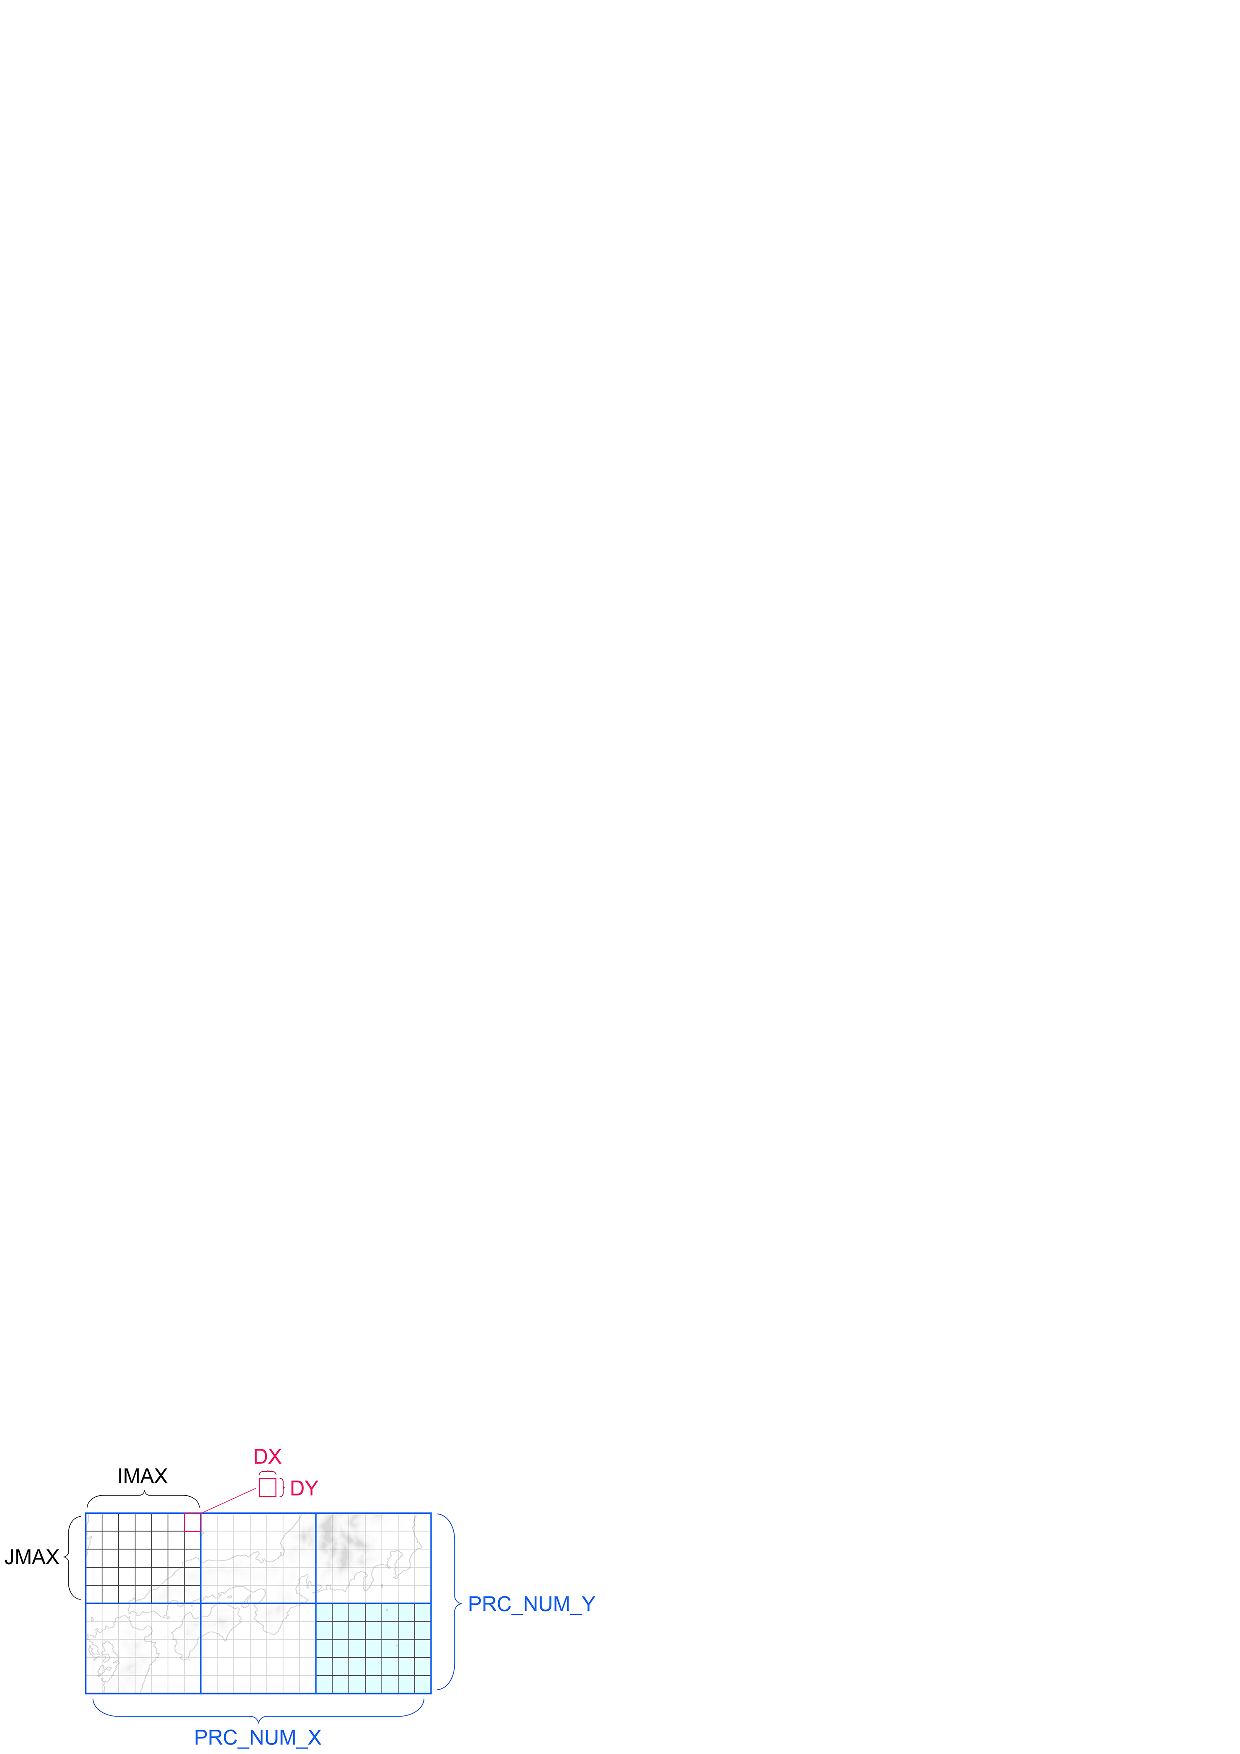
\includegraphics[width=0.8\hsize]{./../../figure/domain_decomposition.pdf}\\
  \caption{計算領域全体に対する、水平格子間隔(\nmitem{DX}, \nmitem{DY})、MPIプロセスあたりの格子数(\nmitem{IMAX}, \nmitem{JMAX})、総格子数(\nmitem{IMAXG}, \nmitem{JMAXG})、MPIプロセス数(\nmitem{PRC_NUM_X}, \nmitem{PRC_NUM_Y})の関係。青色の領域は、1つのMPIプロセスが担当する領域に対応する。}
  \label{fig:domain}
\end{center}
\end{figure}

%-----------------------------------------------------------------------
\subsection{\SubsecGridNumSettng} \label{subsec:relation_dom_reso3}
%-----------------------------------------------------------------------

格子数は、設定ファイル(\verb|***.conf|)の\namelist{PARAM_ATMOS_GRID_CARTESC_INDEX}で指定する。
\editboxtwo{
\verb|&PARAM_ATMOS_GRID_CARTESC_INDEX| & \\
\verb| KMAX  = 97,|  & ; 鉛直層数 \\
\verb| IMAXG = 40,|  & ; {\XDIR}の格子点数 \\
\verb| JMAXG = 25,|  & ; {\YDIR}の格子点数 \\
\verb|/|\\
}

%-----------------------------------------------------------------------
\subsection{\SubsecGridIntvSettng} \label{subsec:gridinterv}
%-----------------------------------------------------------------------

第\ref{subsec:buffer}節で述べる緩和領域を除いて水平格子間隔は等間隔でのみ設定できるが、
鉛直格子間隔は任意に設定できる。
全方向について格子間隔を等間隔で設定する場合には、
\namelist{PARAM_ATMOS_GRID_CARTESC}内の\nmitem{DX, DY, DZ}にそれぞれ、
東西、南北、鉛直方向の格子間隔を指定する(単位は[m])。
\editboxtwo{
\verb|&PARAM_ATMOS_GRID_CARTESC| & \\
\verb| DX = 500.D0,| & ; {\XDIR} の格子間隔\\
\verb| DY = 500.D0,| & ; {\YDIR} の格子間隔\\
\verb| DZ = 500.D0,| & ; {\ZDIR}(鉛直方向)の格子間隔\\
\verb|/|\\
}

鉛直方向に対しては、任意の等間隔でない格子を指定することができる。
モデルは C 格子系を採用しており、
速度ベクトルと他のスカラー量に対する定義点は半格子分ズレている。
ここでは、スカラー量の位置をセンターポイントと呼び、
それから半格子ズレた位置をフェイスポイントと呼ぶ。
鉛直格子点のフェイスポイントを\namelist{PARAM_ATMOS_GRID_CARTESC}内の\nmitem{FZ(:)}に配列として与えることができる
\footnote{この場合には、シミュレーションで用いられたものと同じ浮動小数点の精度を用いることが望ましい。
デフォルトでは、モデルは倍精度の浮動小数点を使用するとしてコンパイルされる。
}。
詳細は図\ref{fig:scale_grid}を参照されたい。
また、\nmitem{FZ(:)}で指定する要素の数は、鉛直層数
(\namelist{PARAM_ATMOS_GRID_CARTESC_INDEX}内の\nmitem{KMAX})と一致している必要があることに注意が必要である。
例として、理想実験の設定ファイルを下記に示す。
\editboxtwo{
\verb|&PARAM_ATMOS_GRID_CARTESC|     & \\
\verb| DX = 500.D0,|   & {\XDIR} の格子間隔(等間隔) [m]\\
\verb| DY = 500.D0,|   & {\YDIR}の格子間隔(等間隔) [m]\\
\verb| FZ(:) = |       & {\ZDIR}のフェイスポイントの位置 [m] \\
\verb|    80.000000000000000D0      ,| & \\
\verb|    168.00000190734863D0      ,| & \\
\verb|    264.80000610351567D0      ,| & \\
\verb|     〜 中略 〜|           & \\
\verb|    14910.428862936289D0      ,| & \\
\verb|    15517.262523292475D0      ,| & \\
\verb|    16215.121232702089D0      ,| & \\
\verb|    17017.658748523147D0      ,| & \\
\verb|    17940.576891717363D0      ,| & \\
\verb|    19001.932756390710D0      ,| & \\
\verb|    20222.492000765058D0      ,| & \\
\verb| BUFFER_DZ = 5000.D0,|          & 第\ref{subsec:buffer}節参照\\
\verb| BUFFFACT  =   1.0D0,|          & 第\ref{subsec:buffer}節参照\\
\verb|/|\\
}

\begin{figure}[tb]
\begin{center}
  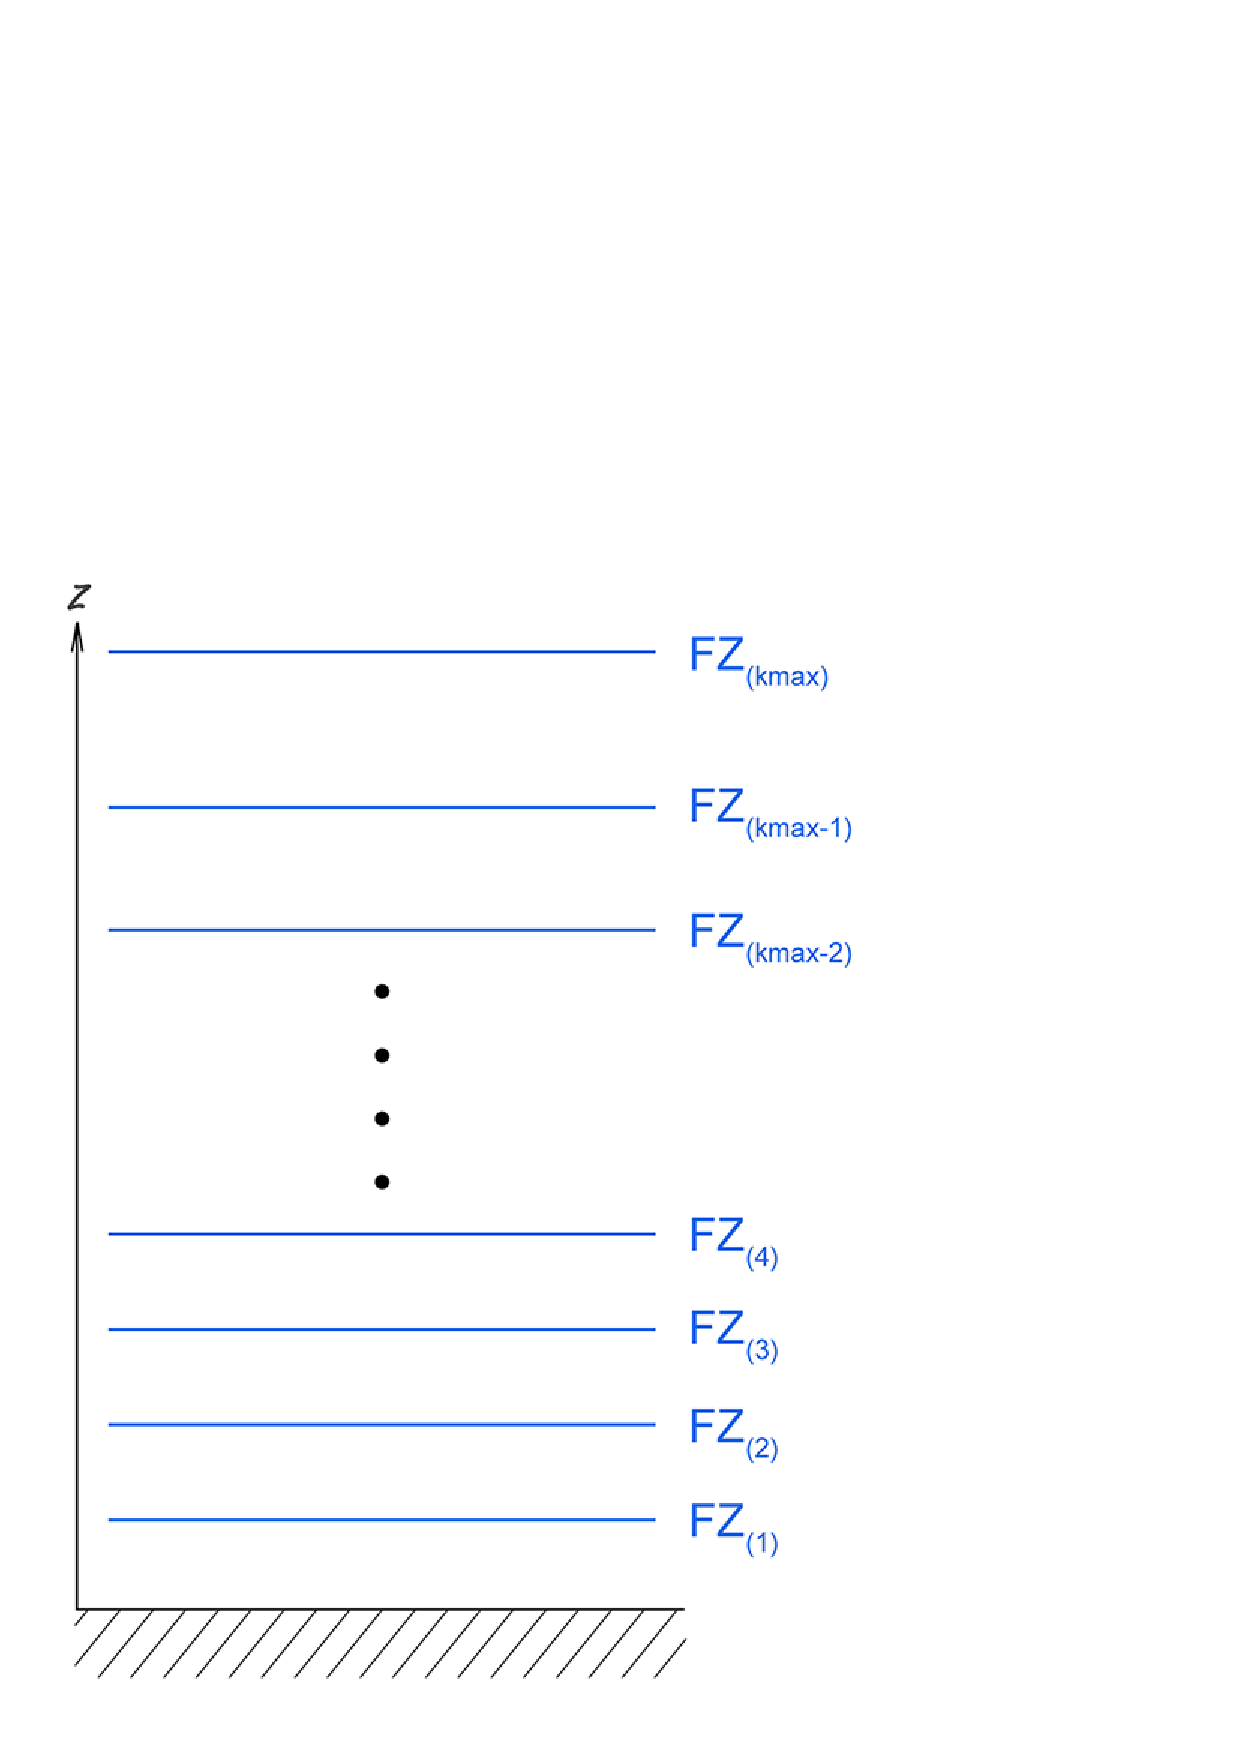
\includegraphics[width=0.4\hsize]{./../../figure/verticalface.pdf}\\
  \caption{\scalerm におけるフェイスポイントの定義点。
  \namelist{PARAM_ATMOS_GRID_CARTESC}で\nmitem{FZ}を指定する時は、
  $k=1$での値として第1層目上端の高さを与える。$k=1$での値は地表面の高さでないことに注意が必要である。}
  \label{fig:scale_grid}
\end{center}
\end{figure}

上記の設定は、標高 0 m の場所での値として扱われる。
地形が存在する場所での鉛直格子点の位置は、地形に沿った座標系によって適切に取り扱われる。


鉛直格子点の位置は任意に設定できるが、変わった設定をすると計算不安定がしばしば生じる。
これを避けるために、ディレクトリ\texttt{scale-\version/scale-rm/util/makevgrid/}の中に
\verb|make_vgrid.f90|というFortranプログラムと幾つかのネームリストの例を用意している。
必要があれば参考として用いることができる。
このツールは\nmitem{FZ(:)}の値を直接出力するので、コピーして設定ファイルに貼り付けるなどして利用可能である。

%-----------------------------------------------------------------------
\subsection{\SubsecMPIProcess} \label{subsec:relation_dom_reso2}
%-----------------------------------------------------------------------

MPIプロセス数は設定ファイルの\namelist{PARAM_PRC_CARTESC}内で指定する。
\editboxtwo{
\verb|&PARAM_PRC| & \\
\verb| PRC_NUM_X       = 2,| & ; {\XDIR}(東西方向)のMPI並列分割数 \\
\verb| PRC_NUM_Y       = 1,| & ; {\YDIR}(南北方向)のMPI並列分割数 \\
\verb|/|\\
}
MPIプロセス数は、\XDIR および \YDIR それぞれについて
総格子点数 \nmitem{IMAXG}, \nmitem{JMAXG} の約数でなければならない。
そうでなければ、プログラムは以下のメッセージを出力して直ちに終了する。
\msgbox{
  \verb|number of IMAXG should be divisible by PRC_NUM_X| \\
}
or
\msgbox{
  \verb|number of JMAXG should be divisible by PRC_NUM_Y| \\
}.

MPI プロセスの総数は、\verb|PRC_NUM_X| $\times$ \verb|PRC_NUM_Y|  によって与えられる。
上記の例では、\XDIR に領域を2分割し、\YDIR には領域を分割しないので、
2-MPI 並列ということになる。
ジョブを投げる際のMPIコマンドに指定するMPIプロセス数として、この総プロセス数を与える必要がある。
この条件を満たさない場合には、プログラムは計算を行わずに直ちに終了し、
下記のメッセージが標準出力に出力される。
\msgbox{
\verb|xxx total number of node does not match that requested. Check!| \\
}

\scalerm の入出力ファイルはMPIプロセス毎に分割されているため、
分割ファイルの総数はMPIプロセス数によって変化する。
例えば、2-MPI並列用に作成した初期値ファイルは、
4-MPI並列のモデル実行には使用できない。
MPIプロセス数を変更する場合は、
\verb|pp.conf|、\verb|init.conf|、\verb|run.conf| 内の
\namelist{PARAM_PRC_CARTESC}を編集し、
\verb|pp|、\verb|init| の過程を再度行う必要がある。
もしくは、後処理ツール \sno を利用して、ファイルの再分割を行うことも可能である
(第\ref{sec:sno}節参照)。

%-----------------------------------------------------------------------
\subsection{\SubsecRayleighDampingSetting} \label{subsec:raydamp}
%-----------------------------------------------------------------------

\scalerm は高度座標を採用している。
最上層の境界条件は剛体壁であり、モデル上端において音波や重力波がしばしば反射する。
反射波の悪影響を軽減するために、モデル領域の上部に「スポンジ層」と呼ばれる減衰層を設ける。
スポンジ層内では、レイリー摩擦によって鉛直速度を減衰させる。
緩和の時定数(e-folding time)はモデル上端で最も短く、高度が下がるにつれて長くする。
スポンジ層の下端より下では、緩和の時定数は無限大に設定する。
スポンジ層の厚さの指定方法は2種類あり、\namelist{PARAM_ATMOS_DYN}で設定する。
\begin{enumerate}
\item スポンジ層の層数を指定\\
  \nmitem{ATMOS_DYN_wdamp_layer} でスポンジ層の層数を指定する。
  この層数はモデル上端から数える。
\item スポンジ層の下端高度[m]の指定\\
  \nmitem{ATMOS_DYN_wdamp_height} で指定した高度よりも上部にある層を、スポンジ層として設定する。
\end{enumerate}

デフォルトでは上記のパラメータは両方とも設定されず、スポンジ層は適用されない、
両方が指定された場合は、\nmitem{ATMOS_DYN_wdamp_layer} が優先される。

スポンジ層上端での緩和の時定数は、\nmitem{ATMOS_DYN_wdamp_tau} で設定する(単位は秒)。\\
これには\nmitem{TIME_DT_ATMOS_DYN}よりも小さな値は設定できない。
時定数を陽に指定しない場合は、\nmitem{TIME_DT_ATMOS_DYN} の10倍の値が自動で設定される。
\nmitem{TIME_DT_ATMOS_DYN}については、第\ref{sec:timeintiv}節を参照されたい。
また、具体的な設定例は、第\ref{subsec:atmos_dyn_scheme}節を参照されたい。

%鉛直格子を一定間隔に設定する(第\ref{subsec:gridinterv}節参照)場合にも、スポンジ層の格子間隔は大きくとって鉛直格子数を節約したいという要望があるだろう。
%この場合は次の第\ref{subsec:buffer}節で説明するように、鉛直方向の緩和領域を設定し、緩和領域の格子間隔をストレッチする方法を用いる。

%レイリーダンピングの係数は、以下の式で計算される。
%\[
%  \nmitemeq{wdamp_coef}_{(k)} = \left\{ \begin{array}{ll}
%    \frac{1}{2 \times \nmitemeq{wdamp_tau}} ( 1 - \cos ( \pi \times \frac{ FZ_{(k)} - \nmitemeq{wdamp_height} }{ FZ_{(kmax)} - \nmitemeq{wdamp_height} } ) ) & (FZ_{(k)} \ge \nmitemeq{wdamp_height}) \\
%    0 & (FZ_{(k)} \lt \nmitemeq{wdamp_height})
%  \end{array} \right.
%\]

%-----------------------------------------------------------------------
\subsection{\SubsecBasicBufferSetting} \label{subsec:buffer}
%-----------------------------------------------------------------------

一般に水平境界では、境界条件として与えられる入力データと
実際の計算で得られる出力データの間に値の不一致が起こる。
計算において、この不一致は非物理的なモード等の幾つかの問題を生じさせる。
この問題を回避するために、領域内に「緩和領域」を設ける。

図\ref{fig:buff_xz}に示すように、\scalerm では計算領域のすぐ内側に緩和領域を設置する。
緩和領域では、境界値データや親モデルのデータによって指定した値にある時定数で近づけるように、
予報変数を更新する。この緩和を以下ではナッジングと呼ぶ。

\subsubsection{緩和領域}
緩和領域の幅は、設定ファイルの\namelist{PARAM_ATMOS_GRID_CARTSC}の中で設定する。
この設定は全ての手順で共通していなければならないことを再度注意する。
緩和領域の幅を設定する方法は、以下の2種類がある。
\begin{enumerate}
\item \nmitem{BUFFER_NX, BUFFER_NY, BUFFER_NZ} によって緩和領域とする格子数を指定\\
\item \nmitem{BUFFER_DX, BUFFER_DY, BUFFER_DZ} によって緩和領域の幅(参考値)[m]を指定\\\
\end{enumerate}
デフォルトでは上記のパラメータは両方とも指定されず、緩和領域は設定されない。
また、両方が指定された場合は、格子数による指定が優先される。
水平方向には東西南北の四方境界に緩和領域が設定されるが、鉛直方向には領域上端にのみ緩和領域が設定され、下端には設定されない。
緩和領域は計算領域の内側に設定されるため、
ナッジングの影響を受けない実際の対象領域(緩和領域を除いた範囲)は
計算領域よりも狭くなることに注意が必要である。

以下に2種類の設定例を示す。
%
\editboxtwo{
\verb|&PARAM_ATMOS_GRID_CARTESC | & \\
 \verb|BUFFER_NX = 30,   | & ; {\XDIR}(東西方向)の緩和領域の格子数\\
 \verb|BUFFER_NY = 30,   | & ; {\YDIR}(南北方向)の緩和領域の格子数\\
 \verb|BUFFFACT  = 1.D0, | & ; 全方向の緩和領域内の格子間隔に対するストレッチ係数(デフォルトは1.0)\\
\verb|/|\\
}
%
\editboxtwo{
\verb|&PARAM_ATMOS_GRID_CARTESC | & \\
 \verb|BUFFER_DZ  =   5000.D0, | & ; {\ZDIR}(モデル上端から下向き方向)の緩和領域の幅(参考値) [m]\\
 \verb|BUFFER_DX  = 300000.D0, | & ; {\XDIR}(東西方向)の緩和領域の幅(参考値) [m]\\
 \verb|BUFFER_DY  = 300000.D0, | & ; {\YDIR}(南北方向)の緩和領域の幅(参考値) [m]\\
 \verb|BUFFFACT_Z = 1.20D0,    | & ; {\ZDIR}の緩和領域内の格子間隔に対するストレッチ係数\\
 \verb|BUFFFACT_X = 1.05D0,    | & ; {\XDIR}の緩和領域内の格子間隔に対するストレッチ係数\\
 \verb|BUFFFACT_Y = 1.05D0,    | & ; {\YDIR}の緩和領域内の格子間隔に対するストレッチ係数\\
\verb|/|\\
}

{\XDIR}の緩和領域の設定方法を以下で説明する。
緩和領域の格子数 \verb|ibuff|は、\nmitem{BUFFER_NX}に等しい。
\nmitem{BUFFER_NX}を用いずに\nmitem{BUFFER_DX}で指定した場合は、\verb|ibuff|は
\[
\sum_{n=1}^{\verb|ibuff|} \verb|BDX|(n) \ge \nmitemeq{BUFFER_DX} \nonumber
\]
の関係を満たす最小の整数であるように自動的に計算される。
したがって、緩和領域の幅 $\verb|BUFFER|_{\verb|X|}$ ($= \sum_{n=1}^{\verb|ibuff|} \verb|BDX|(n)$)
は \nmitem{BUFFER_DX} と一致するとは限らないことに注意が必要である。
最後に、緩和領域を除いた計算領域の大きさは、
\[
\nmitemeq{DX} \times ( \nmitemeq{IMAXG} - 2 \times \verb|ibuff| )
\]
と表現される。
{\YDIR}、{\ZDIR}についても同様に設定されるが、
{\ZDIR} の実際の対象領域は、
\[
\nmitemeq{DZ} \times ( \nmitemeq{KMAX} - \verb|kbuff| )
\]
と表現される。
ここで、\verb|kbuff|はモデル上端の緩和領域の格子数である。


\begin{figure}[t]
\begin{center}
  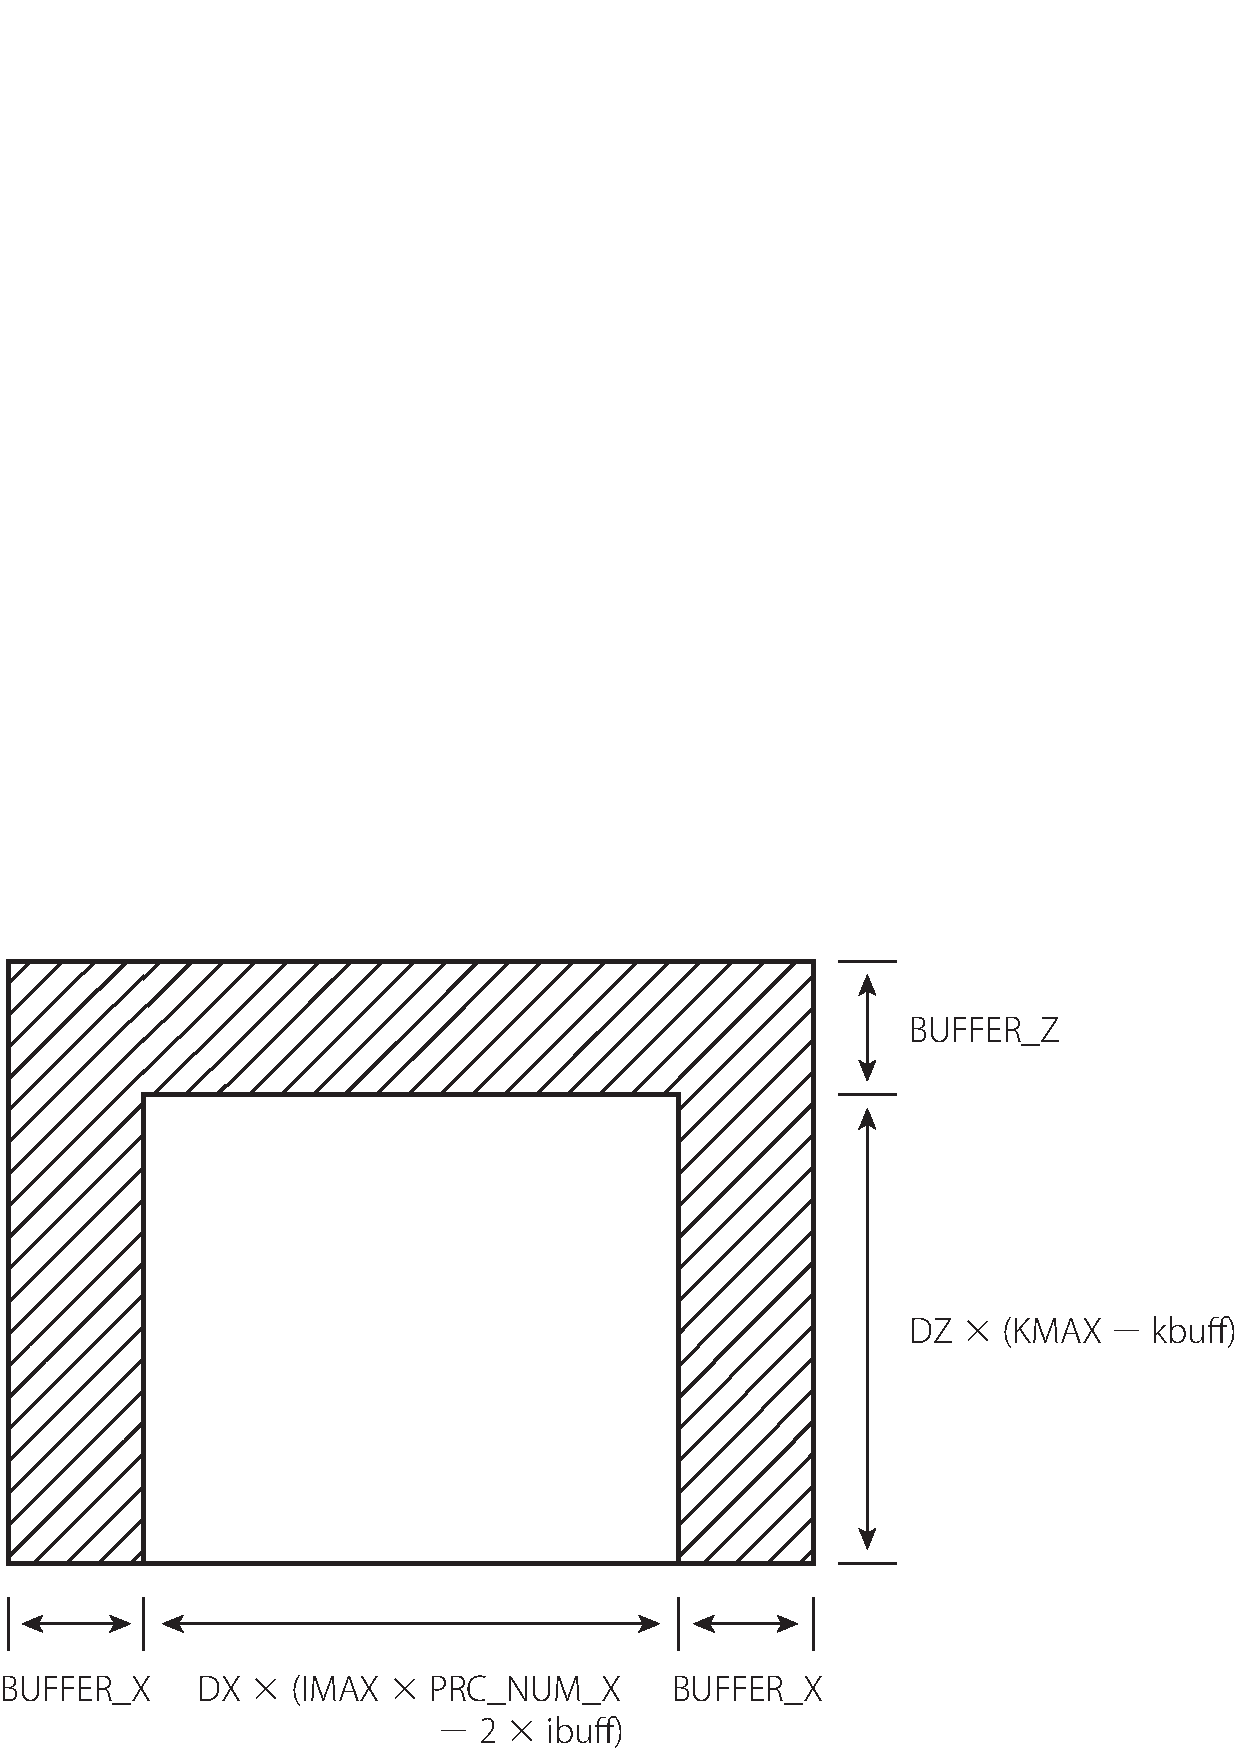
\includegraphics[width=0.8\hsize]{./../../figure/buffer_xz.pdf}\\
  \caption{全計算領域内での緩和領域の配置:斜線部分が緩和領域を意味する。
  図はXZ断面を示しているが、YZ断面についても同様である。}
  \label{fig:buff_xz}
\end{center}
\end{figure}

一般に、緩和領域の幅の設定や格子の置き方には明確な指標はない。
これらの設定は解く問題に依存する。
\scalerm では、モデル上部における鉛直方向の緩和領域の格子点数は5点以上、
側面境界の緩和領域の格子点は20〜40点程度を推奨している。
実験によっては、さらに緩和領域の格子点を増やしたり、
適切なストレッチ係数を用いて緩和領域自体を広げたり、
緩和の時定数を調整したりする必要があるだろう。
緩和の時定数については、以下で説明する。
%\namelist{PARAM_ATMOS_BOUNDARY}の中の
%\nmitem{ATMOS_BOUNDARY_taux, ATMOS_BOUNDARY_tauy, ATMOS_BOUNDARY_tauz}によって秒単位で設定する。
%\nmitem{ATMOS_BOUNDARY_taux, ATMOS_BOUNDARY_tauy}によって秒単位で設定する。
%デフォルトの値は、\nmitem{TIME_DT}の10倍であり、これは、10タイムステップで$1/e$になることに相当する。
%タイムステップについては、第\ref{sec:timeintiv}節を参照のこと。

%-----------------------------------------------------------------------
%\subsubsection{緩和領域における格子間隔のストレッチ設定}
%-----------------------------------------------------------------------

緩和領域の格子間隔は、デフォルトでは
\namelist{PARAM_ATMOS_GRID_CARTESC}の中の\nmitem{DX, DY, DZ}で指定した通りである。
ただし、\nmitem{BUFFFACT}に1以上に設定することによって、ストレッチさせることもできる。
格子間隔を等間隔で指定した場合は、この\nmitem{BUFFFACT}の設定は全方向に対して適用される。
各方向で別々に設定したい場合は、\nmitem{BUFFFACT_X, BUFFFACT_Y, BUFFFACT_Z}を指定する。
\nmitem{FZ(:)}を与えることで鉛直レベルを指定した場合(第\ref{subsec:gridinterv}節参照)は、
上記のストレッチの設定は{\ZDIR}には適用されない。

緩和領域内の格子間隔 (\verb|BDX|) は次の通り決定される。
\begin{eqnarray}
 \verb|BDX(|n\verb|)| &=& \verb|DX| \times \verb|BUFFFACT|^n \nonumber
\end{eqnarray}
ここで、$n$は緩和領域内の格子点番号を表し、計算領域の内側から外側へ向う番号である。
緩和領域の格子間隔は、
\nmitem{BUFFFACT=1.0}とした場合は内部領域と同じであり、
\nmitem{BUFFFACT=1.2}とした場合は内部から外側の領域に向かって1.2倍の割合で広がっていく。
\nmitem{BUFFFACT}の値は任意に設定できるが、計算不安定を避けるために 1.0から1.2 までの値が推奨される。

最後に、緩和領域の大きさ$\verb|BUFFER|_{\verb|X|}$は、
\[
  \verb|BUFFER|_{\verb|X|} = \nmitemeq{DX} \times \frac{ \nmitemeq{BUFFFACT}^{\texttt{\detokenize{ibuff}}}-1}{ \nmitemeq{BUFFFACT}-1 }
\]
となる。
%
緩和領域の幅\nmitem{BUFFER_DX}を同じに設定した場合でも、
\nmitem{BUFFFACT}を大きくすると緩和領域の格子数は少なくなる。
\nmitem{BUFFER_NX}を与えた場合は、緩和領域の幅のみが変わる。

\subsubsection{緩和領域におけるナッジングの方法}

緩和領域におけるナッジングの設定は、\namelist{PARAM_ATMOS_BOUNDARY}内のパラメータで行う。
境界データの種類は、\namelist{PARAM_ATMOS_BOUNDARY}内の\nmitem{ATMOS_BOUNDARY_TYPE}によって設定する(表\ref{tab:nml_atmos_boundary_type})。

\begin{table}[h]
\begin{center}
\caption{境界値データの種類の選択}
\label{tab:nml_atmos_boundary_type}
\begin{tabularx}{150mm}{lXX} \hline
  \rowcolor[gray]{0.9} 値 & 種類の説明 \\ \hline
  \verb|NONE|    & ナッジングしない \\
  \verb|CONST|   & 指定された定数値にナッジングする \\
  \verb|INIT|    & 初期値にナッジングする \\
  \verb|OFFLINE| & ファイルから読み込んだ値にナッジングする(時間変化なし) \\
  \verb|REAL|    & 親モデルまたは親領域の値にナッジングする(時間変化あり) \\
  \hline
\end{tabularx}
\end{center}
\end{table}


以下は、\namelist{PARAM_ATMOS_BOUNDARY}内のパラメータである。
%
\editboxtwo{
  \verb|&PARAM_ATMOS_BOUNDARY | & \\
  \verb| ATMOS_BOUNDARY_TYPE = 'NONE',         | & ; 境界値データの種類。表\ref{tab:nml_atmos_boundary_type}を参照。 \\
  \verb| ATMOS_BOUNDARY_IN_BASENAME = '',      | & ; 境界値データのファイル名 (\verb|OFFLINE| または\verb|REAL| type の場合)\\
  \verb| ATMOS_BOUNDARY_IN_CHECK_COORDINATES | \textbackslash \\
  ~~\verb|                   = .true.,| & ; 境界データファイル内の座標変数を確認するかのフラグ \\
%    \\ ({\small\slshape 次のページへ続く})
%}
%\editboxtwo{
%  ({\small\slshape 前のページからの続き}) \\ \\
  \verb| ATMOS_BOUNDARY_OUT_BASENAME = '',     | & ; 初期の境界値データを出力するファイル名 \\
  \verb| ATMOS_BOUNDARY_OUT_TITLE | \textbackslash \\
  ~~\verb|     = 'SCALE-RM BOUNDARY CONDITION',| & ; 出力ファイルに対するタイトル \\
  \verb| ATMOS_BOUNDARY_OUT_DTYPE = 'DEFAULT', | & ; 出力のデータ型(\verb|REAL4| or \verb|REAL8|) \\
  \verb| ATMOS_BOUNDARY_USE_DENS = .false.,    | & ; 密度に対するナッジングのスイッチ \\
  \verb| ATMOS_BOUNDARY_USE_VELZ = .false.,    | & ; wに対するナッジングのスイッチ. \\
  \verb| ATMOS_BOUNDARY_USE_VELX = .false.,    | & ; uに対するナッジングのスイッチ. \\
  \verb| ATMOS_BOUNDARY_USE_VELY = .false.,    | & ; vに対するナッジングのスイッチ. \\
  \verb| ATMOS_BOUNDARY_USE_PT = .false.,      | & ; $\theta$に対するナッジングのスイッチ. \\
  \verb| ATMOS_BOUNDARY_USE_QV = .false.,      | & ; 水蒸気に対するナッジングのスイッチ. \\
  \verb| ATMOS_BOUNDARY_USE_QHYD = .false.,    | & ; 水物質に対するナッジングのスイッチ. \\
  \verb| ATMOS_BOUNDARY_VALUE_VELZ = 0.0D0,    | & ; wの値 (\verb|CONST| type の場合のみ) \\
  \verb| ATMOS_BOUNDARY_VALUE_VELX = 0.0D0,    | & ; uの値 (\verb|CONST| type の場合のみ) \\
  \verb| ATMOS_BOUNDARY_VALUE_VELY = 0.0D0,    | & ; vの値 (\verb|CONST| type の場合のみ) \\
  \verb| ATMOS_BOUNDARY_VALUE_PT = 300.0D0,    | & ; $\theta$の値 (\verb|CONST| type の場合のみ) \\
  \verb| ATMOS_BOUNDARY_VALUE_QTRC =   0.0D0,  | & ; 水蒸気の値 (\verb|CONST| type の場合のみ) \\
  \verb| ATMOS_BOUNDARY_ALPHAFACT_DENS = 1.0D0,| & ; 密度に対する$1/\tau$の係数. \\
  \verb| ATMOS_BOUNDARY_ALPHAFACT_VELZ = 1.0D0,| & ; wに対する係数. \\
  \verb| ATMOS_BOUNDARY_ALPHAFACT_VELX = 1.0D0,| & ; uに対する係数. \\
  \verb| ATMOS_BOUNDARY_ALPHAFACT_VELZ = 1.0D0,| & ; vに対する係数. \\
  \verb| ATMOS_BOUNDARY_ALPHAFACT_PT = 1.0D0,  | & ; $\theta$に対する係数. \\
  \verb| ATMOS_BOUNDARY_ALPHAFACT_QTRC = 1.0D0,| & ; 水蒸気に対する係数. \\
  \verb| ATMOS_BOUNDARY_SMOOTHER_FACT = 0.2D0, | & ; 点ごとの差に対する水平方向の平滑化の係数. \\
  \verb| ATMOS_BOUNDARY_FRACZ = 1.0D0,         | & ; z方向の緩和領域に対するナッジング領域の割合. \\
  \verb| ATMOS_BOUNDARY_FRACX = 1.0D0,         | & ; x方向の割合. \\
  \verb| ATMOS_BOUNDARY_FRACY = 1.0D0,         | & ; y方向の割合. \\
  \verb| ATMOS_BOUNDARY_TAUZ = DT * 10.0D0,    | & ; 上端境界でのナッジングの時定数 (秒). \\
  \verb| ATMOS_BOUNDARY_TAUX = DT * 10.0D0,    | & ; 東西境界でのナッジングの時定数 (秒). \\
  \verb| ATMOS_BOUNDARY_TAUY = DT * 10.0D0,    | & ; 南北境界でのナッジングの時定数 (秒). \\
  \verb| ATMOS_BOUNDARY_LINEAR_V = .false.,    | & ; z方向に関するナッジングの時定数分布の種類. \verb|.true.|であれば線形分布、そうでなければサイン型の分布.\\
  \verb| ATMOS_BOUNDARY_LINEAR_H = .false.,    | & ; x, y 方向に関するナッジングの時定数分布の種類. \verb|.true.|であれば線形分布、そうでなければ指数関数分布. \\
  \verb| ATMOS_BOUNDARY_EXP_H = 2.0D0,         | & ; 指数関数分布の場合における指数の係数. \\
  \verb| ATMOS_BOUNDARY_DENS_ADJUST = .true.,  | & ; 質量フラックス調整に対するスイッチ. \\
  \verb| ATMOS_BOUNDARY_DENS_ADJUST_TAU | \textbackslash \\
  ~~\verb|     = -1.0D0,                       | & ; 質量フラックス調整が有効な場合の密度ナッジングの時定数 (秒). \\
}

ナッジングによる時間変化率は、
\begin{eqnarray}
  \left.\frac{\partial \phi_{k,i,j}}{\partial t}\right|_\mathrm{nudging}
  & = & - \alpha \Delta\phi_{k,i,j} \\ \nonumber
  && + \alpha_s \left( \frac{\Delta\phi_{k,i-1,j} + \Delta\phi_{k,i+1,j} + \Delta\phi_{k,i,j-1} + \Delta\phi_{k,i,j+1}}{8} - \frac{\Delta\phi_{k,i,j}}{2} \right),
\label{eq:nudging}
\end{eqnarray}
と書かれる。
ここで、$\Delta\phi$ は境界値データとの差であり、
$\alpha_s = \alpha \times \nmitemeq{ATMOS_BOUNDARY_SMOOTHER_FACT}$である。
$\alpha$は3方向に対する係数$\alpha_x, \alpha_y,\alpha_z$の最大値である。
これらの係数は、以下のような長さスケール$e$に依存する。
\begin{equation}
  e = \max\left( 1 - \frac{d}{\texttt{BUFFER} \times \nmitemeq{ATMOS_BOUNDARY_FRAC}}, 0 \right),
\end{equation}
ここで、$d$は境界からの距離である。
もし\nmitem{ATMOS_BOUNDARY_LINEAR_V}が\verb|.true.|であれば、
\begin{equation}
  \alpha_z = e_z / \tau_z,
\end{equation}
\verb|.false.|であれば、
\begin{equation}
  \alpha_z =  \sin^2(\pi e_z/2) / \tau_z,
\end{equation}
である。
ここで、 $\tau_z$は\nmitem{ATMOS_BOUNDARY_TAUZ}である。
水平方向については、\nmitem{ATMOS_BOUNDARY_LINEAR_H}が\verb|.true.|であれば、
\begin{equation}
  \alpha_x = e_x / \tau_x,
\end{equation}
\verb|.false.|であれば、
\begin{equation}
  \alpha_x = e_x \exp\{ - (1-e_x) \times \nmitemeq{ATMOS_BOUNDARY_EXP_H} \} / \tau_x.
\end{equation}
である。
$\alpha_y$は$\alpha_x$と同様の方法によって導かれる。

$\tau$は境界($d=0$)での緩和時間であり、計算された値と境界値の差はこの時間スケールで$1/e$倍となる。
他方、式\ref{eq:nudging}の右辺2項目によって、$\Delta \phi$の two-grid スケールの成分は\\ $\tau/\nmitemeq{ATMOS_BOUNDARY_SMOOTHER_FACT}$の時間で$1/e$倍となる。
$\tau$のデフォルトの値は、\nmitem{TIME_DT}の10倍である。
\nmitem{TIME_DT}については第\ref{sec:timeintiv}節を参照されたい。


\namelist{PARAM_ATMOS_BOUNDARY}の\nmitem{ATMOS_BOUNDARY_TYPE}が ``\verb|REAL|'' の時、\\
\nmitem{ATMOS_BOUNDARY_USE_{VELX,VELY,PT,QV,DENS}}の設定に関わらず、
水平速度・温位・水蒸気・密度に対する上部および側面境界でのナッジングが適用される。
加えて \nmitem{ATMOS_BOUNDARY_USE_VELZ} と \nmitem{ATMOS_BOUNDARY_USE_QHYD} が \verb|.true.| の場合、それぞれ鉛直速度および水凝結物に対するナッジングが適用される。
オンライン・ネスティング(第\ref{subsec:nest_online}節を参照)の子領域として
計算が行われる場合、
境界での親データの扱いは、上記の``\verb|REAL|''と同様の設定が適用される。
ただし、\nmitem{ATMOS_BOUNDARY_USE_VELZ} と \nmitem{ATMOS_BOUNDARY_USE_QHYD}の代わりに、
\namelist{PARAM_COMM_CARTESC_NEST} の \nmitem{ONLINE_USE_VELZ} および \nmitem{ONLINE_BOUNDAYR_USE_QHYD} で指定する。


密度のナッジングは、側面境界値に対する計算領域での質量バイアスを軽減するために有用である。
一方で、密度ナッジングの適用は、緩和領域での気圧傾度力を減少させる。
この結果、特に流出域において、気圧傾度力によって境界値情報をドメイン内部に伝える効果も弱まる。
この効果(気圧傾度)を維持したまま、質量バイアスを軽減させる方法として、
側面境界における質量フラックスの調整が可能である。これを適用することで、密度ナッジングを弱くすることができる。
%
\nmitem{ATMOS_BOUNDARY_DENS_ADJUST} を \verb|.true.| とすると、
親モデルと\scale の計算領域の間の全領域総質量の差が小さくなるように、側面境界質量フラックスが調整される。
例えば、シミュレーションにおける全質量が親モデルの質量に比べて小さい場合は、西境界における $\rho u$ および南境界における $\rho v$ を増加、東境界における $\rho u$ および北境界における $\rho v$ を減少させることで、全質量収束を増加させる。
側面質量フラックス調整は、境界の種類として\verb|REAL|を用いた場合およびオンライン・ネスティングの子領域においてのみ利用可能である。
質量フラックス調整が有効な場合の密度ナッジングの時定数は \nmitem{ATMOS_BOUNDARY_DEN_ADJUST_TAU} で設定する。
負の値が設定された場合は、内部で境界値データの $1/6$ と設定される。
密度ナッジングを弱めるためには、この時定数を \nmitem{ATMOS_BOUNDARY_TAUX} や \nmitem{ATMOS_BOUNDARY_TAUY} よりも大きな値に設定する。
\scalerm における質量フラックス調整方法は、側面境界における質量フラックスによる全質量変化が、降水や地表面潜熱フラックス等の物理過程による質量変化に比べて十分大きいという仮定のもとで作られている。
この仮定が妥当であるかどうかは、対象とするドメインや状況による。


上端境界の周辺における同様な減衰のさせ方として、レイリー摩擦が存在する(第 \ref{subsec:raydamp}節を参照)。

%-----------------------------------------------------------------------
\subsection{\SubsecGridOceanLandUrban} \label{subsec:gridolu}
%-----------------------------------------------------------------------

海洋/陸/都市モデルの水平格子は、大気モデルの設定と共通である。
すなわち、水平格子数は\namelist{PARAM_ATMOS_GRID_CARTESC_INDEX}の\nmitem{IMAXG, JMAXG}で指定され、
水平格子間隔は \\ \namelist{PARAM_ATMOS_GRID_CARTESC}の\nmitem{DX, DY}で指定される。
一方、鉛直格子についてはそれぞれ個別の設定が必要である。

海洋モデルの鉛直格子設定については、第~\ref{sec:basic_usel_ocean}~節、
陸モデルの鉛直格子設定については、第~\ref{sec:basic_usel_land}~節、
都市モデルの鉛直格子設定については、第~\ref{sec:basic_usel_urban}~節を参照のこと。

% 完了
  \clearpage
  \section{\SecMapprojectionSetting} \label{subsec:adv_mapproj}
%------------------------------------------------------
\scalerm では、格子点は実距離に基づいて配置される。
各格子点での緯度・経度の値は、基準位置の緯度経度を与えることによって、ある地図投影法から計算される。
格子の緯度・経度に関する情報は、SCALE が生成するNetCDF形式の全出力ファイルに含まれる。
計算領域の位置と地図投影法は、\nmitem{PARAM_MAPPROJECTION}で設定できる。
この設定は、\textcolor{blue}{\texttt{pp.conf}、\texttt{init.conf}、\texttt{run.conf}の設定ファイル間で一致させなければならない}。
上記の設定例を以下に示す。
\editboxtwo{
\verb|&PARAM_MAPPROJECTION| & \\
\verb| MAPPROJECTION_basepoint_lon = 138.727778D0,| & \\
\verb| MAPPROJECTION_basepoint_lat = 35.360556D0,|  & \\
\verb| MAPPROJECTION_type          = 'MER',|        & ; 表\ref{tab:map_proj}から選択.\\
\verb|/| & \\
}

\begin{table}[h]
\begin{center}
\caption{\scalerm で選択可能な地図投影法}
\begin{tabularx}{150mm}{|l|X|} \hline
 \rowcolor[gray]{0.9} \verb|MPRJ_type| & 地図投影法 \\ \hline
 \verb|NONE| & 地図投影なし(理想実験用)、デフォルト \\ \hline
 \verb|LC|   & ランベルト正角円錐図法              \\ \hline
 \verb|PS|   & ポーラーステレオ図法                \\ \hline
 \verb|MER|  & メルカトル図法                     \\ \hline
 \verb|EC|   & 正距円筒図法                       \\ \hline
\end{tabularx}
\label{tab:map_proj}
\end{center}
\end{table}

\noindent
\nmitem{MPRJ_basepoint_lat, MPRJ_basepoint_lon}は、
それぞれ基準点の緯度・経度である。
デフォルトの設定では、基準点は計算領域の中心である。
\scalerm では、北緯を正、南緯を負の値として表現し、
東経を正、西経を負の値として表現する。
経度は180度以上の値を用いて表現することができる。
上記の設定では、計算領域の中心が北緯35.360556度、東経138.727778度に設定されている。
計算領域の全体は、指定された大きさでこの場所を中心にして配置される。

\nmitem{MAPPROJECTION_type}は地図投影法の種類を表しており、\verb|MER|はメルカトル図法を意味する。
表\ref{tab:map_proj}は、\scalerm で現在選択できる地図投影法を示している。
メルカトル図法の場合には、投射する円筒に接する基準緯線を\nmitem{MAPPROJECTION_M_lat}で設定する(単位は度)。
一般的に基準緯線は赤道にとることが多い。
しかし、メルカトル図法は基準緯線に近いほど歪みが少なく正確であるので、
\scalerm では、\nmitem{MAPPROJECTION_M_lat}を陽に指定しなければ
\nmitem{MAPPROJECTION_basepoint_lat}を基準緯線として用いる。

次に、地図投影法の中でも利用頻度が高い、ランベルト正角円錐図法の設定を以下で説明する。
以下の例は、現実大気実験チュートリアルで使用した\verb|run.d01.conf|ファイル内の記述と同じである。\\

\editbox{
\verb|&PARAM_MAPPROJECTION| \\
\verb| MAPPROJECTION_basepoint_lon = 135.220404,| \\
\verb| MAPPROJECTION_basepoint_lat = 34.653396,| \\
\verb| MAPPROJECTION_type          = 'LC',| \\
\verb| MAPPROJECTION_LC_lat1       =  30.0,| \\
\verb| MAPPROJECTION_LC_lat2       =  40.0,| \\
\verb|/| \\
}
\scalerm では、2標準緯線型の投影方法を採用している。
南側、北側の標準緯線はそれぞれ\nmitem{MAPROJECTION_LC_lat1, MAPROJECTION_LC_lat2}で指定する(単位は[度])。
両標準緯線に挟まれた領域では、経線に対する緯線の長さの比が、地球の楕円体面上での長さの比と近くなるように調節される。

さらに下記のように設定すれば、基準点(\nmitem{MAPROJECTION_basepoint_x, MAPROJECTION_basepoint_y})を、
デフォルト設定である計算領域の中心からずらすことができる。\\~\\
\editbox{
\verb|&PARAM_MAPPROJECTION| \\
\verb| MAPPROJECTION_basepoint_lon = 135.220404,| \\
\verb| MAPPROJECTION_basepoint_lat = 34.653396,| \\
\verb| MAPPROJECTION_basepoint_x   = 100.0,| \\
\verb| MAPPROJECTION_basepoint_y   = 100.0,| \\
\verb| MAPPROJECTION_type          = 'LC',| \\
\verb| MAPPROJECTION_LC_lat1       = 30.0,| \\
\verb| MAPPROJECTION_LC_lat2       = 40.0,| \\
\verb|/| \\
}

地図投影の中心位置は、計算領域の南西端(左下角)からの距離によって指定する。つまり、\\
\nmitem{MAPROJECTION_basepoint_x, MAPPROJECTION_basepoint_y}はそれぞれ、
\XDIR や \YDIR に対する左下角と基準位置の間の距離である(単位は[m])。
これらを指定しない場合は、地図投影の中心は計算領域の中心に設定される。
図\ref{fig:map_lc}に、両方の場合における地図投影の中心と計算領域の関係を示す。


\begin{figure}[t]
\begin{center}
  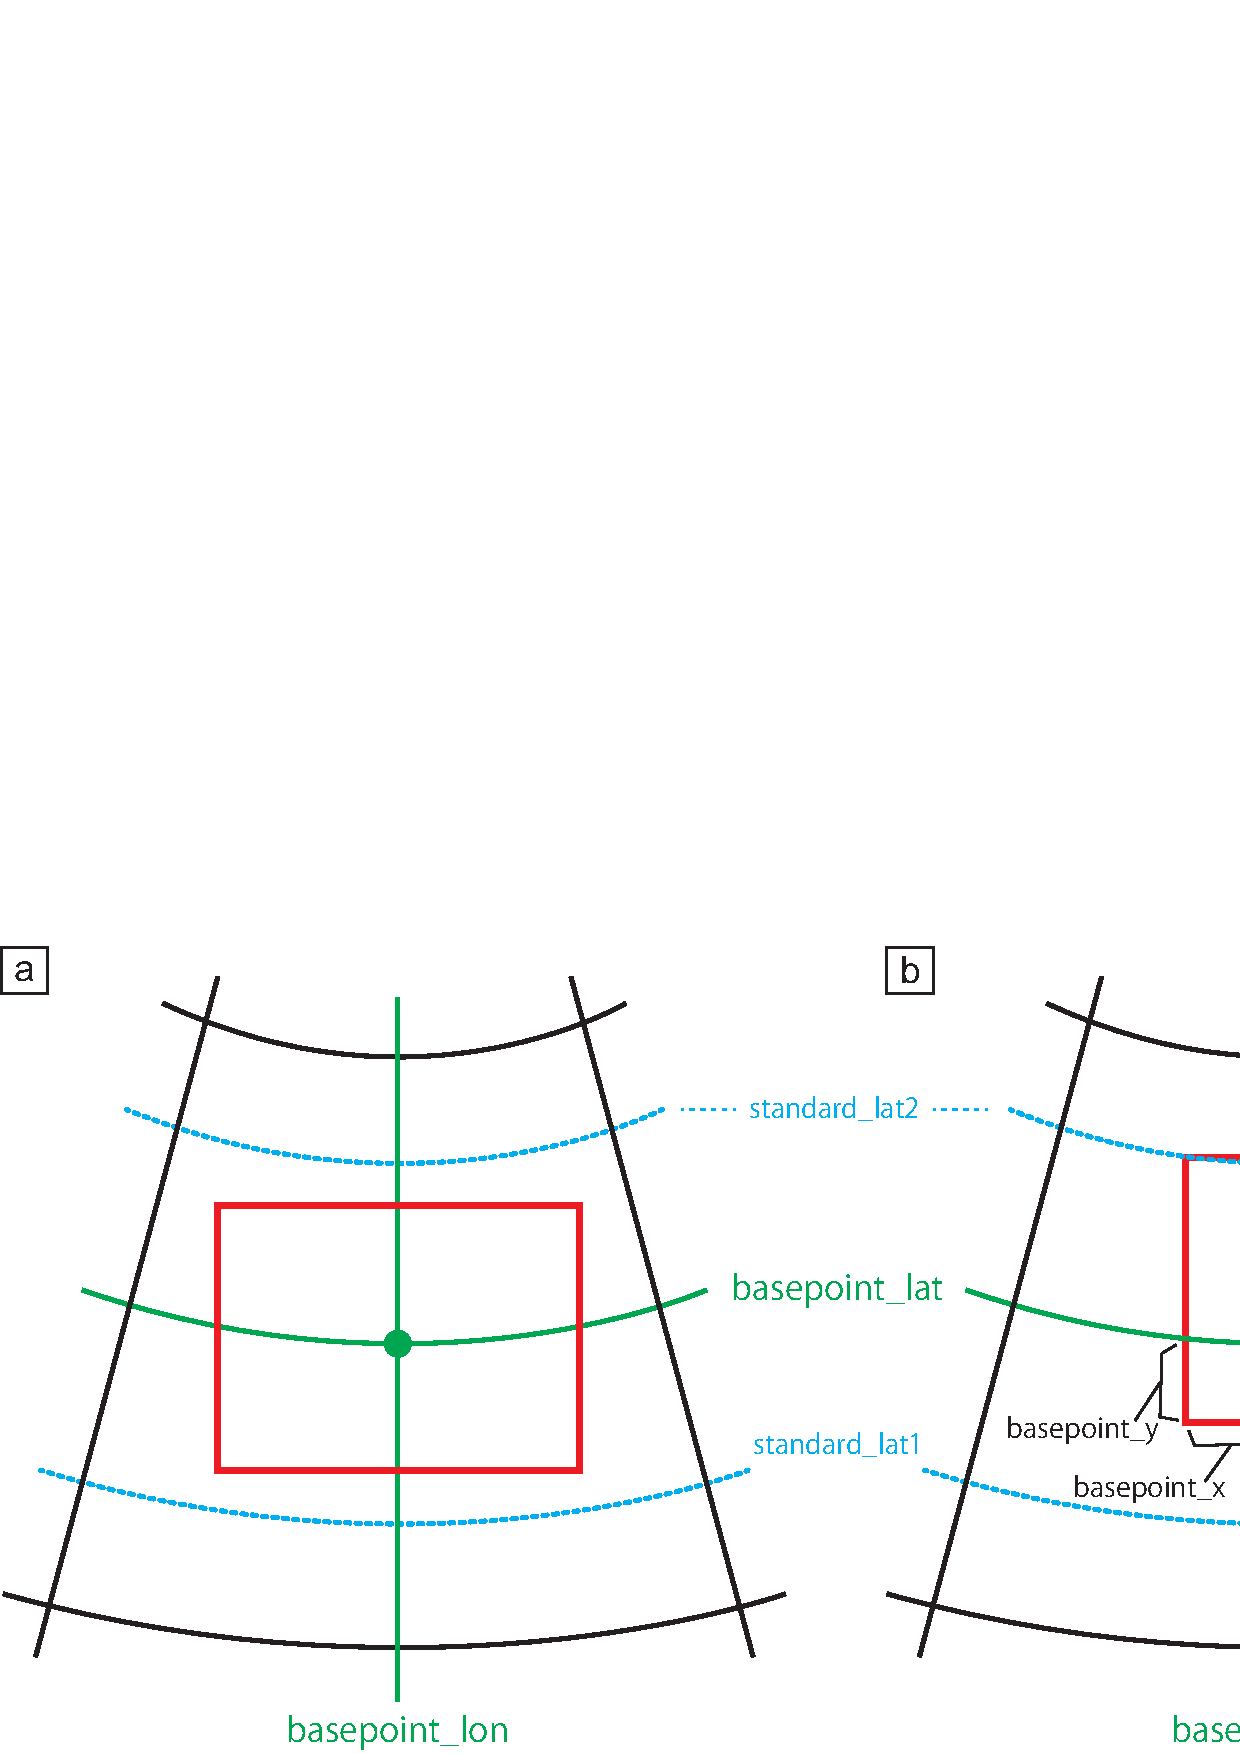
\includegraphics[width=0.8\hsize]{./figure/LC_latlon_xy.pdf}\\
  \caption{投影中心と計算領域の関係:(a)はデフォルト設定の場合、(b)は投影中心の位置を計算領域中心からずらした場合。
  赤線は計算領域の境界を表す。}
  \label{fig:map_lc}
\end{center}
\end{figure}
% 完了
  \section{Setting the topography} \label{subsec:basic_usel_topo}
%-----------------------------------------------------------------------

\scalerm employs the terrain-following coordinates to represent topography.
In these coordinates, the bottom face of the lowest grid is given such that it can follow the surface altitude. The allowable maximum angle of inclination, $\theta_{\max}$[radian] is calculated as follows: 
\begin{eqnarray}
  && \theta_{\max} = \arctan( \mathrm{RATIO} \times \mathrm{DZ}/\mathrm{DX} )\nonumber,
\end{eqnarray}
where $\mathrm{DZ}$ and $\mathrm{DX}$ are the horizontal and vertical grid intervals, respectively.  As shown in the above equation, $\theta_{\max}$ depends on spatial resolution. 
In \scalerm, the default value of $\mathrm{RATIO}$ is 1.0.
If $\mathrm{RATIO}$ is greater than unity, the fine topography is expressed, and vice versa. Note that at $\mathrm{RATIO} >1$, the risk of numerical instability increases.

The program \verb|scale-rm_pp| converts external topography data into \scalelib format.  The detailed configurations are specified in \namelist{PARAM_CNVTOPO} in configuration file \verb|pp.conf|. An example is as follows:
\editboxtwo{
\verb|&PARAM_CNVTOPO  |                  & \\
 \verb|CNVTOPO_name                  = "GTOPO30", | & ; Data name used\\
 \verb|CNVTOPO_smooth_maxslope_ratio = 1.0,       | & ; Allowable maximum ratio of inclination to $\mathrm{DZ}$/$\mathrm{DX}$ \\
 \verb|CNVTOPO_smooth_local          = .true.,    | & ; 
Whether smoothened or not, only grids whose angles of inclination exceed the maximum value \\
 \verb|CNVTOPO_copyparent            = .false.,   | & ; Whether the topography in the buffer region is copied \\
\verb|/|\\
}
\scalerm supports GTOPO30 and DEM50M provided by the Geospatial Information Authority of Japan as external input topography data.

The topographical data is formulated as the area-weighting mean of grid spacing.
This conversion calculates the difference in altitude between them using their neighboring grids and inclinations.
In case $\theta_{\max}$ exceeds the allowable maximum angle of inclination, \\
i.e., \nmitem{CNVTOPO_smooth_maxslope_ratio}, the topography is smoothened by a Laplacian filter with several iterations until the angle is below the allowable maximum angle.
Smoothing is selectively applied either only to grids whose angles of inclination exceed the maximum value, or to the entire domain.
Since the former saves the sharp structure of the topography within the allowable maximum angle, it is selected if the representation of fine structures is desired.
The Gaussian filter is also selected as a smoothing filter. In this case, the topography is smoother than when the Laplacian filter is used.

\nmitem{CNVTOPO_copyparent} is the item used for the nesting computation.
In general, the topography in the child domain is finer than in the parent domain due to higher spatial resolution.
At this time, problems often occers due to 
an inconsistency between 
the atmospheric data in the buffer region of the child domain and that in the parent domain.
To avoid this problem, the topography of the parent domain can be copied to the buffer region of the child domain by specifying \nmitem{CNVTOPO_copyparent}$=$\verb|.true.| If there is no parent domain, \nmitem{CNVTOPO_copyparent} must be \verb|.false.|. Section \ref{subsec:nest_topo} provides a more detailed explanation of the case that involves the use of \nmitem{CNVTOPO_copyparent}.
% 完了
  \clearpage
  %\newpage
\section{\SecBasicIntegrationSetting} \label{sec:timeintiv}
%------------------------------------------------------
積分時間やタイムステップは、実験の目的や設定によって適切に設定する必要がある。
空間解像度を変えた場合はそれに応じたタイムステップを設定する必要があり、
同じ解像度でも計算不安定を防ぐためにタイムステップを短くすることもある。

積分時間とタイムステップの設定は、
設定ファイル\verb|run.conf|の\namelist{PARAM_TIME}の項目を編集することで設定できる。\\

\noindent {\small {\gt
\ovalbox{
\begin{tabularx}{150mm}{lX}
\verb|&PARAM_TIME| & \\
\verb| TIME_STARTDATE             = 2014, 8, 10, 0, 0, 0,| & 計算開始の日付:放射過程を用いる実験等で必要\\
\verb| TIME_STARTMS               = 0.D0,  | & 計算開始時刻[mili sec]\\
\verb| TIME_DURATION              = 12.0D0,| & 積分時間[単位は\verb|TIME_DURATION_UNIT|で設定]\\
\verb| TIME_DURATION_UNIT         = "HOUR",| & \verb|TIME_DURATION|の単位\\
\verb| TIME_DT                    = 60.0D0,| & 時間積分のタイムステップ\\
\verb| TIME_DT_UNIT               = "SEC", | & \verb|TIME_DT|の単位 \\
\verb| TIME_DT_ATMOS_DYN          = 30.0D0,| & 力学過程計算のタイムステップ\\
\verb| TIME_DT_ATMOS_DYN_UNIT     = "SEC", | & \verb|TIME_DT_ATMOS_DYN|の単位\\
\verb| TIME_DT_ATMOS_PHY_MP       = 60.0D0,| & 雲物理過程計算のタイムステップ \\
\verb| TIME_DT_ATMOS_PHY_MP_UNIT  = "SEC", | & \verb|TIME_DT_ATMOS_PHY_MP|の単位\\
\verb| TIME_DT_ATMOS_PHY_TB       = 60.0D0,| & 乱流過程計算のタイムステップ \\
\verb| TIME_DT_ATMOS_PHY_TB_UNIT  = "SEC", | & \verb|TIME_DT_ATMOS_PHY_TB|の単位\\
\verb| TIME_DT_ATMOS_PHY_RD       = 600.0D0, | & 放射過程計算のタイムステップ \\
\verb| TIME_DT_ATMOS_PHY_RD_UNIT  = "SEC",  | & \verb|TIME_DT_ATMOS_PHY_RD|の単位\\
\verb| TIME_DT_ATMOS_PHY_SF       = 60.0D0, | & 大気下端境界(フラックス)過程計算のタイムステップ\\
\verb| TIME_DT_ATMOS_PHY_SF_UNIT  = "SEC",  | & \verb|TIME_DT_ATMOS_PHY_SF|の単位\\
\verb| TIME_DT_OCEAN              = 300.0D0,| & 海面過程計算のタイムステップ\\
\verb| TIME_DT_OCEAN_UNIT         = "SEC",  | & \verb|TIME_DT_OCEAN|の単位\\
\verb| TIME_DT_LAND               = 300.0D0,| & 陸面過程計算のタイムステップ\\
\verb| TIME_DT_LAND_UNIT          = "SEC",  | & \verb|TIME_DT_LAND|の単位\\
\verb| TIME_DT_URBAN              = 300.0D0,| & 都市過程計算のタイムステップ\\
\verb| TIME_DT_URBAN_UNIT         = "SEC",  | & \verb|TIME_DT_URBAN|の単位\\
\verb| TIME_DT_ATMOS_RESTART      = 21600.D0, | & リスタートファイル(大気)の出力間隔\\
\verb| TIME_DT_ATMOS_RESTART_UNIT = "SEC",    | & \verb|TIME_DT_ATMOS_RESTART|の単位\\
\verb| TIME_DT_OCEAN_RESTART      = 21600.D0, | & リスタートファイル(海面)の出力間隔\\
\verb| TIME_DT_OCEAN_RESTART_UNIT = "SEC",    | & \verb|TIME_DT_OCEAN_RESTART|の単位\\
\verb| TIME_DT_LAND_RESTART       = 21600.D0, | & リスタートファイル(陸面)の出力間隔\\
\verb| TIME_DT_LAND_RESTART_UNIT  = "SEC",    | & \verb|TIME_DT_LAND_RESTART|の単位\\
\verb| TIME_DT_URBAN_RESTART      = 21600.D0, | & リスタートファイル(都市)の出力間隔\\
\verb| TIME_DT_URBAN_RESTART_UNIT = "SEC",    | & \verb|TIME_DT_URBAN_RESTART|の単位\\
\verb|/|\\
\end{tabularx}
}}}\\


\nmitem{TIME_DT} は、時間積分計算におけるタイムステップであり、$\Delta t$ と呼ばれることが多い。
トレーサー移流計算のタイムステップとして使われるほか、すべての物理過程計算のタイムステップの基本単位となる。
タイムステップは、計算不安定を起こさないように
格子間隔を移流速度で割った値が取りうる最少値よりも小さな値を設定する。

力学変数の時間積分のためのタイムステップは移流速度ではなく音速で制約されるため、一般には上記のタイムステップよりも小さくとる必要がある。この時間間隔は、\nmitem{TIME_DT_ATMOS_DYN} で設定する。

\nmitem{TIME_DT_ATMOS_DYN}の値は、計算安定性のため主に時間積分スキームに依存し、
\nmitem{ATMOS_DYN_TINTEG_SHORT_TYPE} が \verb|RK4| の場合には
最少格子間隔(HE-VI利用時には水平の最少格子間隔)を 420 m/s で割った値が、
\verb|RK3| の場合には 840 m/s で割った値が目安となる。
ただし、\nmitem{TIME_DT_ATMOS_DYN}は、\nmitem{TIME_DT}の約数である必要があることに注意すること。
また、\nmitem{TIME_DT}の\nmitem{TIME_DT_ATMOS_DYN}に対する比が大きくなりすぎると
計算的に不安定になるケースがあるため、\nmitem{TIME_DT}/\nmitem{TIME_DT_ATMOS_DYN}の比は、2もしくは3に設定することが望ましい。


それぞれの物理過程のタイムステップは各過程が与えるテンデンシーが更新されるタイミングを表す。
各過程は利用される場合、モデルのセットアップ時に一度計算され、テンデンシーが設定される。
その後、各過程に設定した時間間隔でテンデンシーが更新される。時間間隔は\nmitem{TIME_DT}の倍数であることが望ましい。
時間間隔を指定しない場合は、\nmitem{TIME_DT}と同じ値が設定される。

%海面・陸面・都市モデルの内部においても物理過程が存在、各過程のタイムステップでテンデンシーが更新される。

海面・陸面・都市モデルを利用する場合は、大気側で下端境界(フラックス)過程の計算は行われない。
大気は、各地表面過程が計算した状態値・フラックスを海陸フラクションや都市被覆率に応じて重み付け平均された値を受け取る。
このとき、\nmitem{TIME_DT_ATMOS_PHY_SF} は受け取った値をHISTORY出力に渡す時間間隔にのみ用いられるので、
\nmitem{TIME_DT_OCEAN}, \nmitem{TIME_DT_LAND}, \nmitem{TIME_DT_URBAN} と同じか、その約数に設定しておく。

リスタートファイルの出力間隔と、各過程の計算間隔についても気をつけなければいけない。
上で示したとおり、各過程のテンデンシーは必ずセットアップ時に更新される。
そのため、リスタートファイルの出力間隔が
すべての利用する過程の計算時間間隔の倍数になっていない場合、通しで時間積分を行った場合と
途中で停止してリスタートを行った場合の結果に差が生まれる。
時間間隔を指定しない場合は途中で出力はされず、
\nmitem{TIME_DURATION}と同じ時刻、すなわちシミュレーションの最後に出力される。
リスタート計算の設定の詳細は第\ref{sec:restart}節を参照のこと。

    %完了
  \section{\SecBasicOutputSetting} \label{sec:output}
%====================================================================================

計算結果の出力ファイルと出力形式の設定、及び、出力する変数の追加は、
\namelist{PARAM_HISTORY}と\namelist{HISTITEM}で行う。
まず、出力ファイルとデフォルトの出力形式の設定を、\verb|run.conf|の\namelist{PARAM_HISTORY} で行う。\\

\noindent {\small {\gt
\ovalbox{
\begin{tabularx}{150mm}{lX}
\verb|&PARAM_HISTORY| & \\
\verb|  HISTORY_DEFAULT_BASENAME  = "history_d01",| & ; 出力ファイル名の頭。 \\
\verb|  HISTORY_DEFAULT_TINTERVAL = 3600.0,|        & ; 出力の時間間隔。 \\
\verb|  HISTORY_DEFAULT_TUNIT     = "SEC",|         & ; \verb|HISTORY_DEFAULT_TINTERVAL|の単位。 \\
\verb|  HISTORY_DEFAULT_TAVERAGE  = .false.,|       & ; \verb|.false.|: 瞬間値、\verb|.true.|: 時間平均値。\\
\verb|  HISTORY_DEFAULT_ZCOORD    = "model",|       & ; 出力データの鉛直座標の種別。\\
                                                    & ~ \verb|"model"|: モデル面の値を出力。\\
                                                    & ~ \verb|"z"    |: 絶対高度面に内挿した値を出力。\\
                                                    & ~ \verb|"pressure"|: 気圧面に内挿した値を出力。\\
\verb|  HISTORY_DEFAULT_DATATYPE  = "REAL4",|       & ; 出力データの型。\verb|REAL4|, \verb|REAL8|など。\\
\verb|  HISTORY_OUTPUT_STEP0      = .true.,|        & ; 初期時刻(t=0)の値を出力するかどうか。\\
                                                    & ~ \verb|.true.|: 出力、\verb|.false.|: 出力しない。\\
\verb|/| & \\
\end{tabularx}
}}}\\


\nmitem{HISTORY_DEFAULT_TUNIT}の単位は、\\
\verb|"MSEC", "msec", "SEC", "sec", "s", "MIN", "min", "HOUR", "hour", "h", "DAY", "day"|
より選択可能である。
%
\verb|HISTORY_DEFAULT_TAVERAGE = .true.|として、平均値での出力を設定した場合、
出力するタイミング直前の\verb|HISTORY_DEFAULT_TINTERVAL|間の平均値が出力される。

\nmitem{HISTORY_DEFAULT_ZCOORD}で絶対高度面座標(\verb|"z"|)を選択した場合は、
出力データの鉛直層数はモデル面の鉛直層数と同じであり、
各層の高度は標高ゼロ地点でのモデル面高度である。\\
\nmitem{HISTORY_DEFAULT_ZCOORD}で気圧面座標(\verb|"pressure"|)を選択した場合、
\namelist{PARAM_HIST}の\\ \nmitem{HIST_PRES_nlayer}と\nmitem{HIST_PRES}の設定が必要である。

\namelist{PARAM_HIST}の\nmitem{HIST_BND}を\verb|.true.|とした場合、
計算領域の外側のハロ領域のデータも出力される。ただし、周期境界条件の場合にはこの設定は無視される。
\nmitem{HIST_BND}の設定はすべての出力変数に対して適用される。\\

\noindent {\small {\gt
\ovalbox{
\begin{tabularx}{150mm}{lX}
\verb|&PARAM_HIST| & \\
\verb|  HIST_PRES_nlayer   = -1,    |    & ; 層数 (オプション 気圧面出力の場合のみ) \\
\verb|  HIST_PRES          = 0.0,   |    & ; 各層の気圧の値。下層から順に[hPa]で指定する。\\
                                         & ~ (オプション 気圧面出力の場合のみ) \\
\verb|  HIST_BND           = .false.|    & ; 計算領域の外側のハロ領域の値を出力するかどうか。\\
                                         & ~ \verb|.true.|: 出力する, \verb|.false.|: 出力しない.\\
\verb|/| & \\
\end{tabularx}
}}}\\




次に、出力する変数の設定を\namelist{HISTITEM}で行う。
\namelist{HISTITEM}は変数毎に設定するため、出力したい変数の数だけ追加することになる。
それぞれの変数の出力形式は、基本的に \namelist{PARAM_HISTORY} の設定に従うが、
(オプション)のネイムリスとを追加することによって変数毎に変更することも可能である。\\

\noindent {\small {\gt
\ovalbox{
\begin{tabularx}{150mm}{lX}
\verb|&HISTITEM| &\\
\verb| ITEM     = "RAIN",    | &  ; 変数名。 出力可能な変数は付録\ref{achap:namelist}を参照 \\
\verb| BASENAME = "rain_d01",| &  ; (オプション) \verb|HISTORY_DEFAULT_BASENAME|に同じ。\\
\verb| TINTERVAL= 600.0,     | &  ; (オプション) \verb|HISTORY_DEFAULT_TINTERVAL|に同じ。\\
\verb| TUNIT    = "SEC",     | &  ; (オプション) \verb|HISTORY_DEFAULT_TINTERVAL|に同じ。\\
\verb| TAVERAGE = .true.,    | &  ; (オプション) \verb|HISTORY_DEFAULT_TAVERAGE|に同じ。\\
\verb| ZCOORD   = "model",   | &  ; (オプション) \verb|HISTORY_DEFAULT_ZCOORD|に同じ。\\
\verb| DATATYPE = "REAL4",   | &  ; (オプション) \verb|HISTORY_DEFAULT_DATATYPE|に同じ。\\
\verb|/| & \\
\end{tabularx}
}}}\\

(オプション)の項目は、変数\nmitem{ITEM}にのみ適用される。
上記では、明示的にすべての設定を書いているが、
\nmitem{HISTORY_DEFAULT_***} と同じ設定であれば
それらが適用されるので明記する必要はない。
例えば、上記の\namelist{PARAM_HISTORY}の設定に、下記の\namelist{HISTITEM}の設定を組み合わせた場合には、
\verb|history_d01.xxxxxx.nc|に4バイト実数で、3600秒毎に \verb|T, U, V| の瞬間値が出力される。
また、\verb|RAIN|が、600秒の出力間隔で、前600秒間の平均値が出力される。\\

\noindent {\small {\gt
\ovalbox{
\begin{tabularx}{150mm}{l}
\verb|&HISTITEM  ITEM = "T" /|\\
\verb|&HISTITEM  ITEM = "U" /|\\
\verb|&HISTITEM  ITEM = "V" /|\\
\verb|&HISTITEM  ITEM = "RAIN",  TINTERVAL = 600.0, TAVERAGE = .true. /|\\
\end{tabularx}
}}}\\

%%%%%%%%%%%%%%%%%%%%%%%%%%%%%%%%%%%%%%%%%%%%%%%%%%%%%%%%%%%%%%%%%%%%%%%%%%%%%%%%%%%%
 %完了
  \section{How to restart run}\label{sec:restart}
%=======================================================================
The restart function is beneficial to avoid termination of simulations because of the limitation of the job execution time controlled by a computer system.
You can divide a long sequential simulation into multiple runs by restarting. The restart files have the same format as the data generated by the initialization run. The function allows outputting multiple restart files at the specified time interval, not only the end of each simulation.
The settings for the restart files are configured in \namelist{PARAM_RESTART} and \namelist{PARAM_TIME} in \runconf.
The example below indicates that the simulation restarts by the file \verb|restart1_***| and generates restart files \verb|restart2_***| every six hours.

\editboxtwo{
\verb|&PARAM_RESTART                                   | & \\
\multicolumn{2}{l}{\verb| RESTART_IN_BASENAME = "restart1_d01_20070715-000000.000",|} \\
                                                         & Basename of input initial file or restart file. \\
%\verb| RESTART_IN_AGGREGATE          = .false.,        | & Please refer to Section \ref{sec:netcdf} \\
\verb| RESTART_IN_POSTFIX_TIMELABEL  = .false.         | & Add initial date and time after \verb|RESTART_IN_BASENAME|? \\
\verb| RESTART_OUTPUT                = .true.,        | & Output restart file? Default is \verb|.false.| \\
\verb| RESTART_OUT_BASENAME          = "restart2_d01", | & Basename of output restart file. \\
%\verb| RESTART_IN_AGGREGATE          = .false.,        | & Please refer to Section \ref{sec:netcdf} \\
\verb| RESTART_OUT_POSTFIX_TIMELABEL = .true.          | & Add output date and time after \verb|RESTART_OUT_BASENAME|? \\
\verb| RESTART_OUT_TITLE             = "",             | & Title written in the restart file. \\
\verb| RESTART_OUT_DTYPE             = "DEFAULT",      | & \verb|REAL4| or \verb|REAL8| or \verb|DEFAULT| \\
\verb|/                                                | & \\
\\
\verb|&PARAM_TIME| & \\
\verb| TIME_STARTDATE             = 2007, 7, 15, 00, 0, 0,| & Start date of restart run \\
\verb| TIME_STARTMS               = 0.D0,                 | & Start date [ms] \\
\verb| TIME_DURATION              = 12.0D0,               | & Integration time \\
\verb| TIME_DURATION_UNIT         = "HOUR",               | & Unit for \verb|TIME_DURATION| \\
\verb|  ..... *snip* .....                                | & \\
\verb| TIME_DT_ATMOS_RESTART      = 21600.D0,             | & Output interval of restart files for atmospheric variables \\
\verb| TIME_DT_ATMOS_RESTART_UNIT = "SEC",                | & Unit for \verb|TIME_DT_ATMOS_RESTART| \\
\verb| TIME_DT_OCEAN_RESTART      = 21600.D0,             | & Output interval of restart files for ocean variables \\
\verb| TIME_DT_OCEAN_RESTART_UNIT = "SEC",                | & Unit for \verb|TIME_DT_OCEAN_RESTART| \\
\verb| TIME_DT_LAND_RESTART       = 21600.D0,             | & Output interval of restart files for land variables \\
\verb| TIME_DT_LAND_RESTART_UNIT  = "SEC",                | & Unit for \verb|TIME_DT_LAND_RESTART| \\
\verb| TIME_DT_URBAN_RESTART      = 21600.D0,             | & Output interval of restart files for urban variables \\
\verb| TIME_DT_URBAN_RESTART_UNIT = "SEC",                | & Unit for \verb|TIME_DT_URBAN_RESTART| \\
\verb|/| & \\
}

The time intervals for output of restart files are specifided by \nmitem{TIME_DT_ATMOS_RESTART}, \\
\nmitem{TIME_DT_OCEAN_RESTART},  \nmitem{TIME_DT_LAND_RESTART}, and \nmitem{TIME_DT_URBAN_RESTART}.
When they are not specified, the restart files are generated at the end of the simulation, i.e., \nmitem{TIME_DURATION}.
The file names of output restart files are specified by \nmitem{RESTART_OUT_BASENAME}.\\
\nmitem{RESTART_OUT_POSTFIX_TIMELABEL} indicates
whether date and time at output are automatically added to the file name after \nmitem{RESTART_OUT_BASENAME}.\\
The default setting is \nmitem{RESTART_OUT_POSTFIX_TIMELABEL=.true.}.

The restart files are not compatible for all simulation.
The variables included in the restart file are different by the schemes, which chosen in the configuration file.
The simple way for preparing restart files while keeping consistency is to use the same setting for the schemes in a series of the simulations.

The other settings are basically the same as the normal run.
\nmitem{RESTART_IN_BASENAME} is the name of the input file, which includes initial state of the atmosphere and surface sub-models.
The normal run usually uses \verb|init_***| prepared by \verb|scale-rm_init|,
while the restart run uses a restart file output by the previous run.
%
\nmitem{RESTART_IN_POSTFIX_TIMELABEL} is the same as \nmitem{RESTART_OUT_POSTFIX_TIMELABEL},
but for \nmitem{RESTART_IN_BASENAME}.
The default setting is \nmitem{RESTART_IN_POSTFIX_TIMELABEL = .false.}.\\
In avobe example, setting \nmitem{RESTART_IN_BASENAME} \verb|="restart1_d01_20070715-000000.000"| is equivalent to
setting \nmitem{RESTART_IN_POSTFIX_TIMELABEL = .true.} and \nmitem{RESTART_IN_BASENAME} \verb|="restart1_d01"|.
\nmitem{TIME_STARTDATE} and \nmitem{TIME_DURATION} represent the start date and the integration time for the restart simulation.



For a realistic atmospheric experiment, the boundary data prepared by \verb|scale-rm_init|
is needed in addition to the initial data. An example is as follows:

\editboxtwo{
\verb|&PARAM_ATMOS_BOUNDARY                                        | & \\
\verb| ATMOS_BOUNDARY_TYPE        = "REAL",                        | & \verb|"REAL"|: Real case experiment \\
\verb| ATMOS_BOUNDARY_IN_BASENAME = "../init/output/boundary_d01", | & Head of file name of boundary data \\
\verb| ATMOS_BOUNDARY_START_DATE  = 2010, 7, 14, 18, 0, 0,         | & Initial date of boundary file \\
\verb| ATMOS_BOUNDARY_UPDATE_DT   = 21600.D0,                      | & Time interval of boundary data \\
\verb|/                                                            | & \\
}

In the restart simulation, an appropriate date of the boundary data will be read from the boundary file \verb|boundary_***.nc|.
You should specify the first date of the boundary data to \nmitem{ATMOS_BOUNDARY_START_DATE} in \namelist{PARAM_ATMOS_BOUNDARY}.
When \nmitem{ATMOS_BOUNDARY_START_DATE} is not given, the date of the first data in the file is set to the start date of the restart simulation, whether the actual date is different or not.
 %完了
  \clearpage
  \section{\SecAdvanceNesting} \label{sec:nest_exp}
%====================================================================================

ネスティングとは、領域が重複するように複数の計算領域を入れ子(ネスト)構造に設定する方法である。
図\ref{fig_nestsample}は、3つの領域を用いたネスティングの例を示している。
外側の領域は、大きな空間スケールの現象を表現するため、低い水平解像度で広い領域を設定する。
一方、内側の領域は、小さな空間スケールの現象を解像するために、狭い範囲であるが高い水平解像度に設定する。
外側の領域の計算結果は、内側の領域に対する境界値データとして用いられる。
ここでは、
データを渡す外側の領域を「親領域」、データを受ける内側の領域を「子領域」と呼ぶことにする。

ネスティングの方法は下記のように分類される。
\begin{itemize}
\item 実行方法
\begin{description}
 \item[オンライン・ネスティング]\mbox{}\\
計算途中で親領域と子領域の情報を交換しながら、親領域と子領域の計算を同時に実行する方法。
 \item[オフライン・ネスティング]\mbox{}\\
最初に親領域の計算を行って子領域用の初期値・境界値を作成し、
その後に子領域の計算を行う方法。
\end{description}
\item データの受け渡し方法
\begin{description}
 \item[一方向ネスティング]\mbox{}\\
親領域は子領域にデータを送るが、子領域は親領域にデータを送らない。
%つまり、データの流れは親領域から子領域に向かう一方通行。
親領域の結果は、子領域の結果の影響を受けない。
 \item[双方向ネスティング]\mbox{}\\
親領域は子領域にデータを送り、子領域からのデータも受け取る。
したがて、二つの領域の計算は互いに影響し合う。
この方法はオンランイン・ネスティング時に適用できるが、
{\scalerm} v{\version} ではまだ実装されていない。
\end{description}
\end{itemize}

オンラインとオフラインの違いは、親領域から子領域にデータを与える更新頻度にある。
オンライン・ネスティング実験では、子領域の境界条件は親領域の時間刻み幅($\Delta t$)毎に更新される。
オフライン・ネスティング実験では、更新頻度は親領域の計算におけるヒストリファイルの出力間隔に依存する。

ネスティングがオフラインかオンラインかに関わらず、親領域と子領域の格子間隔比($\mathrm{DX}_{\mathrm{d01}}/\mathrm{DX}_{\mathrm{d02}}$)に関してコードの実装上の制限はない。
ただし、この比率が大きすぎると計算結果の物理性能が下がる可能性がある。
\scalerm では、5倍以下で使用することを推奨する。

本節では、親領域の設定ファイルを\verb|***.d01.conf| 、子領域の設定ファイルを\verb|***.d02.conf| と表記する。

\begin{figure}[t]
\begin{center}
  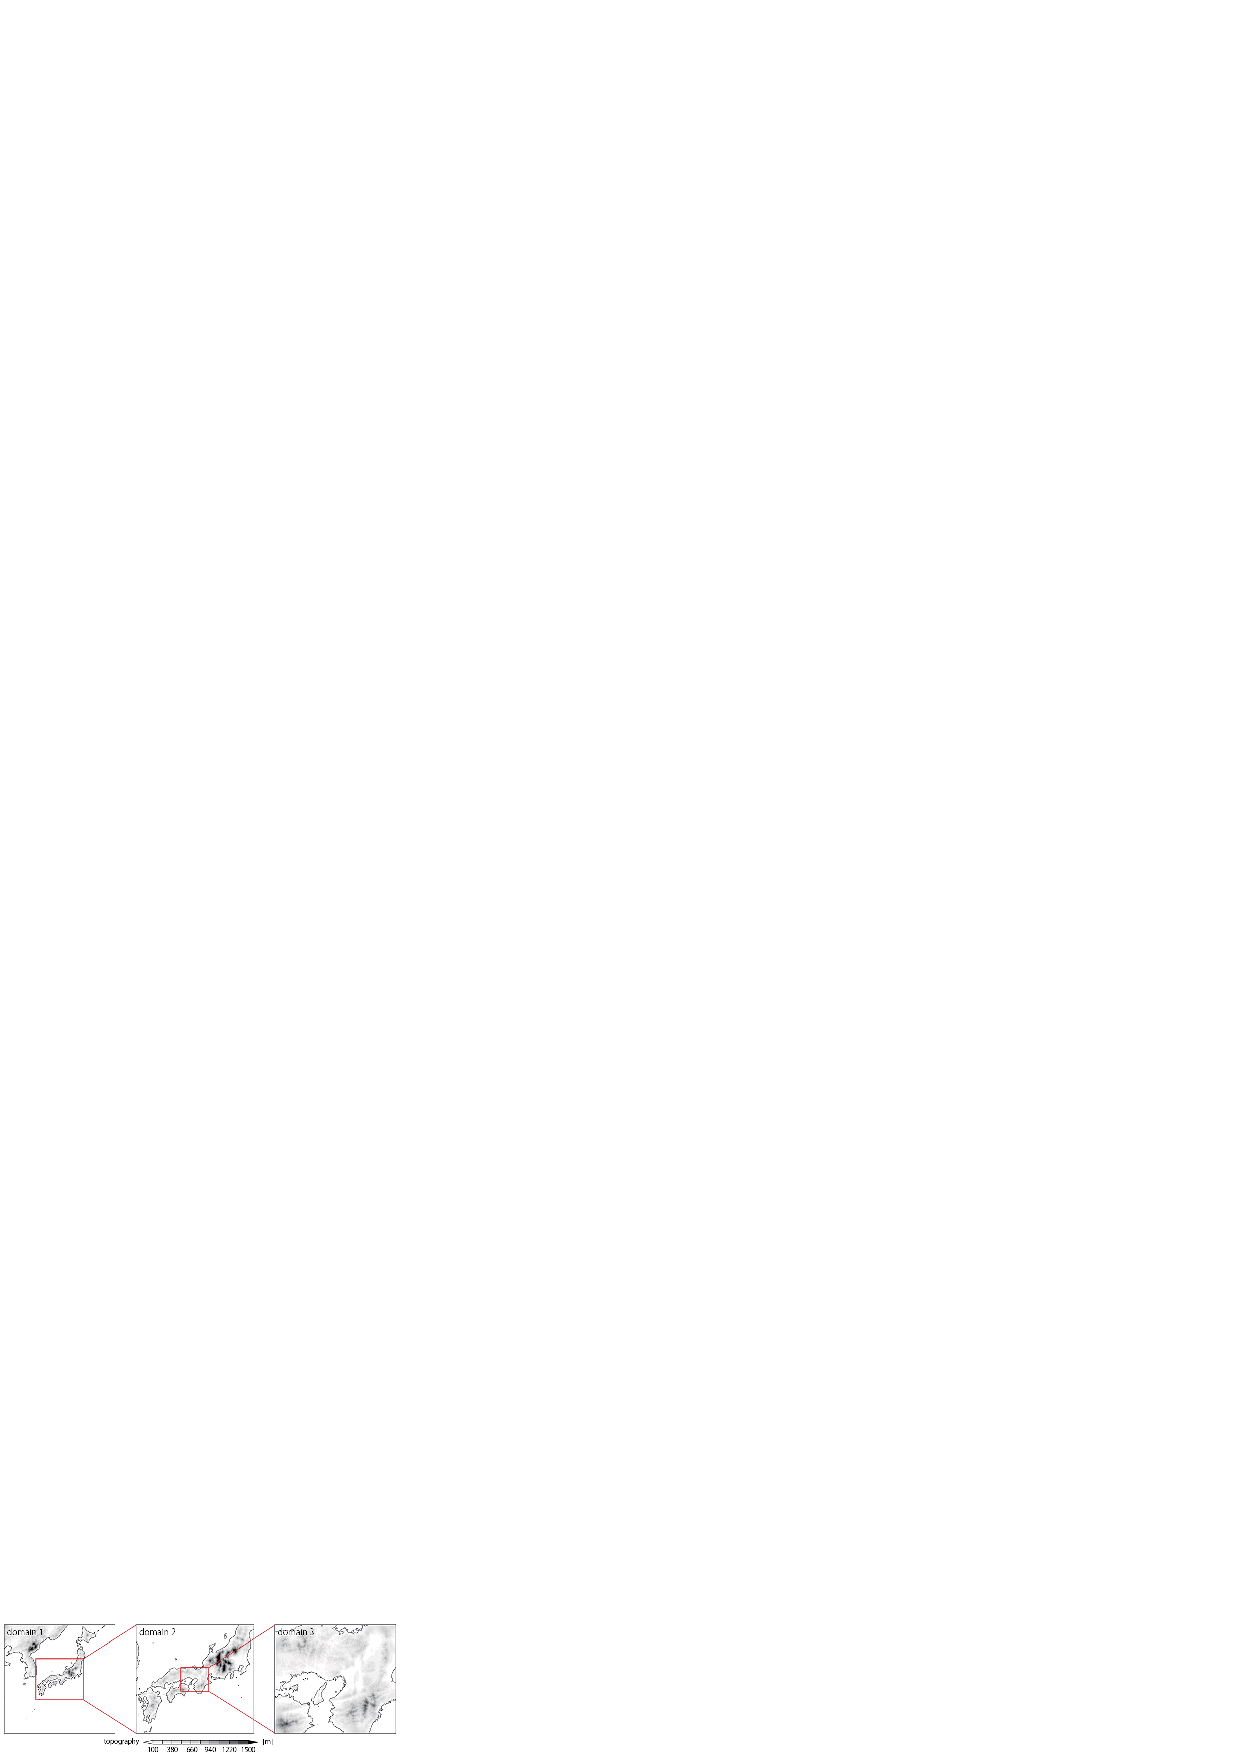
\includegraphics[width=1.0\hsize]{./../../figure/nesting_sample.pdf}\\
  \caption{西日本を対象とした領域ネスティングの例。
    domain 1が最外領域でdomain 3が最内領域である。
    赤い矩形と線は、領域の位置や他の領域との関係を示している。
    水平格子間隔は domain 1 では 7.5 km、domain 2 では 2.5 km、
    domain 3 では 0.5 kmである。}
  \label{fig_nestsample}
\end{center}
\end{figure}
 %完了
  \subsection{Treatment of topography in child domain} \label{subsec:nest_topo}
%------------------------------------------------------
In the nesting experiment, the resolutions of the topography were different between the parent and the child domains due to their different spatial resolutions. In the relaxation area of the child domain (refer to Section \ref{subsec:buffer}), the atmospheric variables were nudged toward those of the parent domain. If the representations of the topography are different between two domains, the reference data for nudging, calculated in the parent domain, often does not exist. In this case, atmospheric data at the missing levels are estimated by extrapolation. However, this may incur error if the estimation by the extrapolation is not accurate.

In order to avoid such inconsistency due to differences in topographies, ``the topography-copy'' function in \scalerm is recommended. This function copies the topography of the parent domain onto that of the child domain in the relaxation area. If this function is used, the topography of the relaxation area in the child domain perfectly corresponds to that in the parent domain, as shown in \ref{fig_topocopy}. To increase the resolution of topography from that in the parent domain to that in the inner domain, the topography transition area is present on the inside of the relaxation area. In the topography transition area, topography is generated by weighing those of the parent and the child domains. By default, the width of the topography transition area is identical to that of the relaxation area. In the inner calculation area, the topography is given by that of the child domain. If ``the making tool for the complete settings of the experiment'' is used ( refer to \ref{sec:basic_makeconf} ), the topography-copy function is automatically applied.

The file \verb|pp.d0*.conf| mentioned in this section can be generated by  ``the making tool for the complete settings of the experiment'' by renaming \\ \verb|${Tutorial_dir}/real/sample/USER.online-nesting.sh| as \verb|USER.sh|. This may help users understand this setting. The configuration and execution methods are explained below.

\begin{figure}[tbh]
\begin{center}
  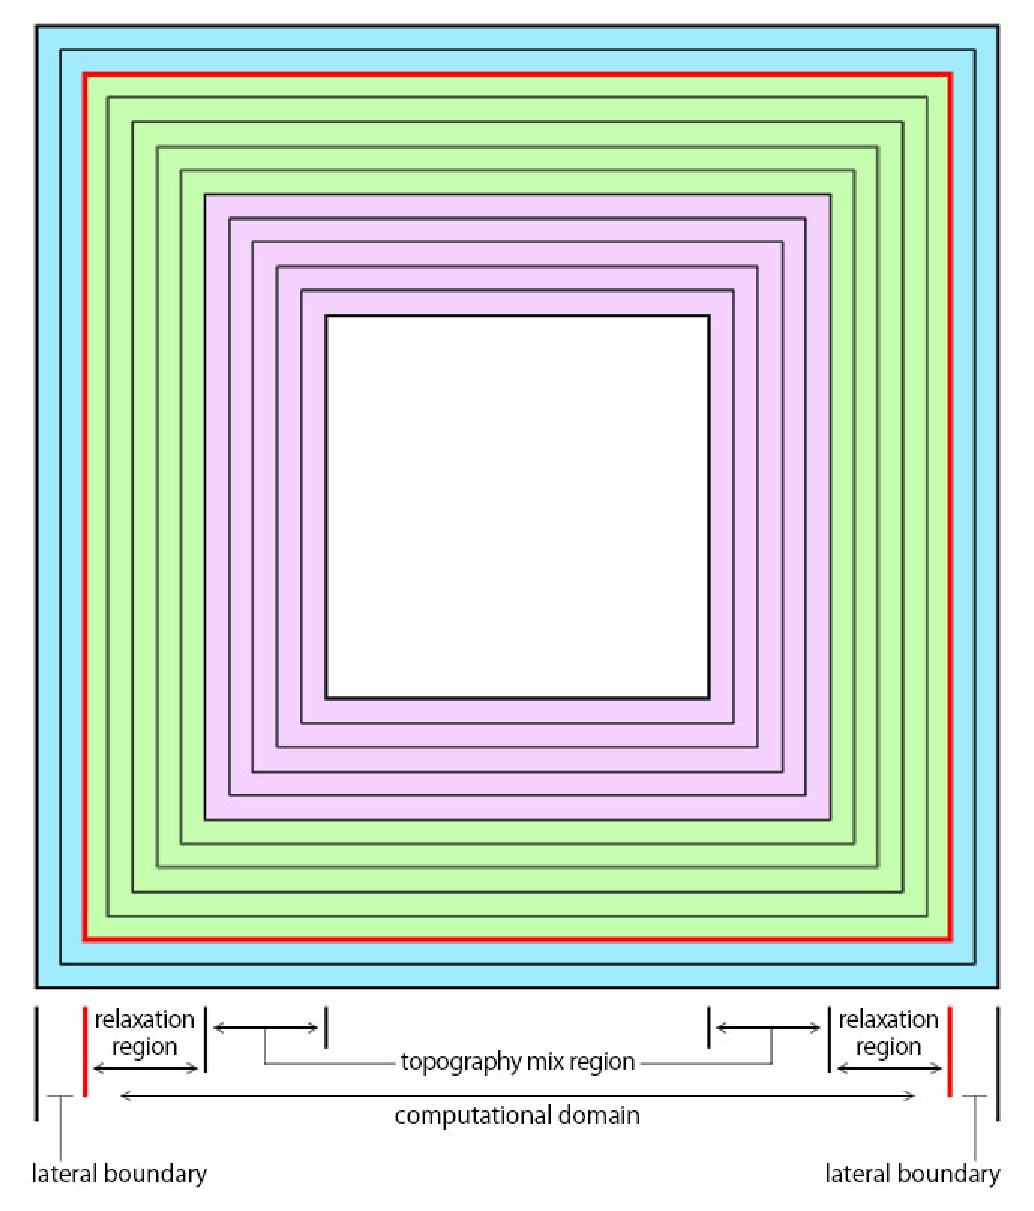
\includegraphics[width=0.4\hsize]{./figure/topo_copy.pdf}\\
  \caption{Horizontal distribution of topography when the topography-copy function is applied.
    The outermost grids shaded in light blue represent the \texttt{HALO} region, and the number of grids depends on
    the horizontal advection scheme. 
    These grids are the lateral boundary. The area demarcated by the red line is the calculation domain.
    The green- and rose-colored areas are the relaxation and the topographical transition areas, respectively.
    The innermost area is where the resolution of topography is the same as that of the original child domain.
    In the topography transition area, topography is altered gradually from that of 
    the parent domain to the original child domain.
}
  \label{fig_topocopy}
\end{center}
\end{figure}



\subsubsection{How to use topography-copy function}

Generate the topography of the parent domain (\verb|scale-rm_pp|) first, and output a catalog file that gives the size of the parent domain to the child domain. The following configuration is needed in \verb|pp.d01.conf| to output a catalog file:
\editboxtwo{
\verb|&PARAM_DOMAIN_CATALOGUE|  & \\
\verb| DOMAIN_CATALOGUE_FNAME  = "latlon_domain_catalogue.d01.txt",| & Name of catalog file\\
\verb| DOMAIN_CATALOGUE_OUTPUT = .true.,| & Whether catalog file is output \\
\verb|/|  & \\
}
The other parameters are the same as usual. 

To use the parent topography for the topography-topo function, edit file \verb|pp.d02.conf| for the child domain as follows.
Here, the output data of topography in the parent domain is assumed to be saved as file \verb|topo_d01.pe***.nc|.
\editboxtwo{
\verb|&PARAM_NEST| & \\
\verb| OFFLINE_PARENT_BASENAME   = "topo_d01", | & base name of the file of the parent domain \\
\verb| OFFLINE_PARENT_PRC_NUM_X  = 2,          | & \verb|PRC_NUM_X| of the parent domain\\
\verb| OFFLINE_PARENT_PRC_NUM_Y  = 2,          | & \verb|PRC_NUM_Y| of the parent domain\\
\verb| LATLON_CATALOGUE_FNAME    = "latlon_domain_catalogue.d01.txt",| & catalog file for the parent domain  \\
\verb|/| &\\
 & \\
\verb|&PARAM_CNVTOPO|  &\\
\verb|     〜 .... 〜| & \\
\verb| CNVTOPO_copy_parent     = .true.,| & whether the topography-copy function is applied\\
\verb|/| &\\
 & \\
\verb|&PARAM_COPYTOPO| & \\
\verb| COPYTOPO_IN_BASENAME   = "topo_d01",| & base name of the file of parent topography data \\
\verb| COPYTOPO_ENTIRE_REGION = .false.,|    & whether the parent’s topography is copied over the entire child domain\\
\verb| COPYTOPO_LINEAR_H      = .true.,|     & \\
\verb|/| & \\
}
If \nmitem{CNVTOPO_copy_parent} in \namelist{PARAM_CNVTOPO} is \verb|.true.|, the topography-copy function is applied.
\nmitem{COPYTOPO_ENTIRE_REGION} is an option whereby the parent’s topography can be copied over the entire child domain. If this is \verb|.true.|, the topography in the child domain is completely copied from that in the parent domain. \nmitem{COPYTOPO_LINEAR_H} is the parameter using which the topography transition method is applied. If \nmitem{COPYTOPO_LINEAR_H} $=$ \verb|.true.|, the mixing ratio of the parent’s topography to the child’s topography is linearly changed. Otherwise, it is changed exponentially.

\subsubsection{Generation of topography}
In case of using the topography-copy function, the generation of the topography should start from the parent domain  because a child domain requires the catalog  file of the parent. If the number of domains is greater than three, the order of execution is as follows: 
\begin{verbatim}
 $ mpirun -n [number of processes] ./scale-rm_pp pp.d01.conf
 $ mpirun -n [number of processes] ./scale-rm_pp pp.d02.conf
 $ mpirun -n [number of processes] ./scale-rm_pp pp.d03.conf
\end{verbatim}


 %完了
  \subsection{\SubsecOflineNesting} \label{subsec:nest_offline}
%------------------------------------------------------

オフラインネスティング実験を行う上での実験設定の制限事項は、以下の2点である。
\begin{itemize}
 \item 子領域の計算範囲は、親領域の計算範囲の内側に位置している必要がある。
 \item 子領域の積分期間は、親領域の積分期間と同じもしくはそれより短い必要がある。
\end{itemize}

~\\
また、オフライン・ネスティング実験の実行過程は次のようになる。
\begin{enumerate}
 \item 親領域の時間積分計算を行う。
 \item 親領域のhistory出力ファイルを用いて子領域の初期値/境界値を作成する。
 \item 作成した初期値/境界値を用いて子領域の時間積分計算を行う。
\end{enumerate}


以下、この流れに沿って説明を進める。
親領域と子領域それぞれについて、\verb|pp.***.conf|、\verb|init.***.conf|、
そして\verb|run.***.conf|ファイルを事前に作成し、
親領域、子領域ともに地形・土地利用データの作成 (\verb|scale-rm_pp|) が、
親領域については、初期値/境界値データの作成 (\verb|scale-rm_init|) が終わっていることを想定して説明を進める。
ここで説明するオフライン・ネスティング実験の設定を記述した設定ファイルは、
サンプル設定ファイル
\verb|${Tutorial_dir}/real/sample/USER.offline-nesting-parent.sh|および
\verb|${Tutorial_dir}/real/sample/USER.offline-nesting-child.sh|
をそれぞれUSER.shに置き換えて、実験セット一式準備ツールを実行すると作成される。
説明を読み進める上で参考にしてもらいたい。

\subsubsection{親領域の時間積分計算を行う}
基本的には通常のシングルドメインの場合と同じ方法で実行すればよいが、
\verb|run.***.conf|の設定で次の5点に注意する必要がある。

\begin{itemize}
 \item 子領域の計算に必要な変数全てを、親領域の計算時にhistory出力する。
 \item 親領域のhistory出力間隔を適度に細かくとること。
 \item 親領域のhistory出力データは、モデル面のデータを出力すること。
 \item 親領域の計算領域を子領域へ伝える「カタログファイル」(以下参照のこと)を出力する。
 \item (子領域の計算開始時刻が親領域と同じ場合) 親領域のhistory出力データにt=0の値を含めること。
\end{itemize}


この設定を\verb|run.d01.conf|に適用すると下記のようになる。
\textcolor{blue}{青文字}で示した部分が、上記の注意点・変更点に対応する部分である。\\

\noindent {\small {\gt
\ovalbox{
\begin{tabularx}{150mm}{lX}
\verb|&PARAM_DOMAIN_CATALOGUE| & \\
\verb| DOMAIN_CATALOGUE_FNAME  = "latlon_domain_catalogue_d01.txt",| & カタログファイルのファイル名\\
\textcolor{blue}{\verb| DOMAIN_CATALOGUE_OUTPUT = .true.,|} & カタログファイルを出力。\\
\verb|/| &\\
 & \\
\verb|&PARAM_HISTORY| &\\
\verb| HISTORY_DEFAULT_BASENAME  = "history",| & \\
\textcolor{blue}{\verb| HISTORY_DEFAULT_TINTERVAL = 900.D0,|} & historyデータの出力時間間隔。\\
\verb| HISTORY_DEFAULT_TUNIT     = "SEC",|   & \verb|HISTORY_DEFAULT_TINTERVAL|の単位。\\
\verb| HISTORY_DEFAULT_TAVERAGE  = .false.,| & \\
\verb| HISTORY_DEFAULT_DATATYPE  = "REAL4",| & \\
\textcolor{blue}{\verb| HISTORY_DEFAULT_ZDIM      = "native",|}  & モデル面データを出力。\\
\textcolor{blue}{\verb| HISTORY_OUTPUT_STEP0      = .true.,|}  & t=0の値を出力に含める。 \\
\verb|/| \\
\end{tabularx}
}}}\\

カタログファイルの出力設定を\verb|.true.|にすると、\verb|latlon_domain_catalogue_d01.txt|というカタログファイルが出力される。
実験セット準備ツールを使用した場合、同ファイルがppディレクトリに出力されているので、そちらを参照すること。
この中には、親領域の計算で各MPIプロセスが担当する計算領域の四隅の緯度・経度が記述されている。
\nmitem{HISTORY_DEFAULT_TINTERVAL}はhistoryデータの出力間隔を示し、
子領域の側面境界条件を更新したい時間間隔に設定する。
短い時間間隔でデータを出力する場合には、ディスクの空き容量にも注意が必要である。
その他、\namelist{PARAM_HISTORY}の各項目の詳細は、第\ref{sec:output}節を参照のこと。

また、子領域の初期値/境界値データ作成に必要な変数全てを
\verb|run.d01.conf|ファイルの\namelist{HISTITEM}に追加しておく必要がある。
オフライン・ネスティングに必要な変数は、下記の通りである。
設定が完了したら、\verb|scale-rm|を実行して親領域の時間積分計算を行う。

\begin{alltt}
  T2, Q2, MSLP, DENS, MOMZ, MOMX, MOMY, RHOT
  LAND_SFC_TEMP, URBAN_SFC_TEMP, OCEAN_SFC_TEMP
  OCEAN_ALB_LW, OCEAN_ALB_SW, LAND_ALB_LW, LAND_ALB_SW
  OCEAN_TEMP, OCEAN_SFC_Z0M, LAND_TEMP, LAND_WATER
(親の雲微物理モデルに合わせて出力; 例えばTomita08なら全て)
  QV, QC, QR, QI, QS, QG
(親の雲微物理モデルに合わせて出力; 例えばTomita08なら不要)
  NC, NR, NI, NS, NG
\end{alltt}



%-------------------------------------------------------------
\subsubsection{親領域の出力ファイルを用いて子領域の初期値/境界値を作成する}
次に、計算が終わった親領域のhistoryデータを用いて、子領域の初期値/境界値を作成する。
実行するプログラムは、通常の初期値/境界値作成と同じ \verb|scale-rm_init| だが、
\verb|init.d02.conf|を下記のように設定する。\\

\noindent {\small {\gt
\ovalbox{
\begin{tabularx}{150mm}{lX}
\textcolor{blue}{\verb|&PARAM_NEST|} & \\
\textcolor{blue}{\verb| USE_NESTING               = .true.,|} & \\
\textcolor{blue}{\verb| OFFLINE                   = .true.,|} & \\
\textcolor{blue}{\verb| OFFLINE_PARENT_PRC_NUM_X  = 2,|}  & \verb|run.d01.conf|の\verb|PRC_NUM_X|\\
\textcolor{blue}{\verb| OFFLINE_PARENT_PRC_NUM_Y  = 2,|}  & \verb|run.d01.conf|の\verb|PRC_NUM_Y|\\
\textcolor{blue}{\verb| OFFLINE_PARENT_KMAX       = 36,|} & \verb|run.d01.conf|の\verb|KMAX|\\
\textcolor{blue}{\verb| OFFLINE_PARENT_IMAX       = 45,|} & \verb|run.d01.conf|の\verb|IMAX|\\
\textcolor{blue}{\verb| OFFLINE_PARENT_JMAX       = 45,|} & \verb|run.d01.conf|の\verb|JMAX|\\
\textcolor{blue}{\verb| OFFLINE_PARENT_LKMAX      = 5,|}  & \verb|run.d01.conf|の\verb|LKMAX|\\
\textcolor{blue}{\verb| LATLON_CATALOGUE_FNAME    = "latlon_domain_catalogue_d01.txt",|} & 親領域を実行した時に作成したカタログファイル\\
\textcolor{blue}{\verb|/|} &\\
 & \\
\verb|&PARAM_MKINIT_REAL_ATMOS| &\\
\textcolor{blue}{\verb| NUMBER_OF_TSTEPS    = 25,|}         & historyファイル内の時間ステップ数\\
\verb| FILETYPE_ORG        = "SCALE-RM",| & \\
\verb| BASENAME_ORG        = "history_d01",|  & \verb|run.d01.conf|の\verb|HISTORY_DEFAULT_BASENAME|\\
\verb| BASENAME_BOUNDARY   = "boundary_d01",| &\\
\textcolor{blue}{\verb| BOUNDARY_UPDATE_DT  = 900.D0,|}     & historyファイルの出力時間間隔(単位は\verb|"SEC"|)\\
\verb|/| &\\
 & \\
\verb|&PARAM_MKINIT_REAL_OCEAN| &\\
\textcolor{blue}{\verb| NUMBER_OF_TSTEPS    = 25,|}         & historyファイル内の時間ステップ数\\
\verb| BASENAME_ORG        = "history_d01",|  & \verb|run.d01.conf|の\verb|HISTORY_DEFAULT_BASENAME|\\
\verb| FILETYPE_ORG        = "SCALE-RM",| & \\
\verb|/| &\\
 & \\
\verb|&PARAM_MKINIT_REAL_LAND| &\\
\textcolor{blue}{\verb| NUMBER_OF_TSTEPS    = 25,|}         & historyファイル内の時間ステップ数\\
\verb| BASENAME_ORG        = "history_d01",|  & \verb|run.d01.conf|の\verb|HISTORY_DEFAULT_BASENAME|\\
\verb| FILETYPE_ORG        = "SCALE-RM",| & \\
\verb|/| &\\
\end{tabularx}
}}}\\


\scalerm の出力データから初期値境界値を作成する場合は、
\nmitem{FILETYPE_ORG}に\verb|"SCALE-RM"|を指定する。
\nmitem{BOUNDARY_UPDATE_DT}は、基本的に、親領域の設定ファイル(\verb|run.d01.conf|)の\\
\nmitem{HISTORY_DEFAULT_TINTERVAL}と同じ設定を記述する。
%
\namelist{PARAM_NEST}の項目は、ネスティング実験のための設定項目である。
オフライン・ネスティングでは、\nmitem{USE_NESTNG=.true., OFFLINE=.true.}と設定する。
\nmitem{OFFLINE_PARENT_***} で始まる6つの設定変数は親領域の設定を記述する変数である。
親領域の設定ファイル(\verb|run.d01.conf|) を参照して正しく設定すること。\\


設定の編集が完了したら、\verb|scale-rm_init|を実行し、子領域の初期値/境界値を作成する。
実行時に下記のようなメッセージが表示されて計算が止まる場合は、
子領域の計算領域が親領域の計算領域の外側に取られている部分がある。
この場合は、各領域の大きさや領域中心の設定を見直す必要がある。\\

\noindent {\small {\gt
\fbox{
\begin{tabularx}{150mm}{l}
\verb|xxx ERROR: REQUESTED DOMAIN IS TOO MUCH BROAD| \\
\verb|xxx -- LONGITUDINAL direction over the limit| \\
\end{tabularx}
}}}\\



\subsubsection{作成した初期値/境界値を用いて子領域の時間積分計算を行う}
初期値/境界値作成が終わったら、子領域の計算 (\verb|scale-rm|) を実行する。
子領域の実行は、通常の現実大気実験と同じである。
1点だけ注意すべき点として、
\verb|run.d02.conf|の\namelist{PARAM_ATMOS_BOUNDARY}の\nmitem{ATMOS_BOUNDARY_UPDATE_DT}が
初期値/境界値作成で使用した親領域のhistoryデータ出力間隔に合っているか確認すること。
現在のところ、この設定に親領域と子領域間で不整合あっても警告やエラーメッセージが発せられないまま、
計算が進み、場合によっては正常終了してしまうため注意が必要である。


\noindent {\small {\gt
\ovalbox{
\begin{tabularx}{150mm}{l}
\verb|&PARAM_ATMOS_BOUNDARY| \\
\verb|     〜 中略 〜|\\
\textcolor{blue}{\verb| ATMOS_BOUNDARY_UPDATE_DT  = 900.D0,|} \\
\verb|/| \\
\end{tabularx}
}}}\\

\noindent
多段のオフライン・ネスティング実験を行いたい場合は、以上の過程を繰り返せばよい。
つまり、子領域として時間積分計算した結果を再度、親領域と見立てて、
さらに内側の孫領域の初期値/境界値作成を行なえばよい。
 %完了
  \subsection{\SubsecOnlineNesting} \label{subsec:nest_online}
%----------------------------------------------------------

オンライン・ネスティング実行時の制約として、
親領域と子領域の積分時間は一致している必要があり、
かつ、親領域の時間ステップは子領域の時間ステップの倍数でなければならない。
一方、親領域と子領域の間で鉛直層数、鉛直レベル、地図投影法、物理スキームは一致している必要はない。

オンライン・ネスティング実験では全ての領域の計算を同時に実行する。
現在は、親領域から子領域に対してデータの受け渡しを行う一方向ネスティングのみをサポートしている。
また、サポートするネスティングの段数は、最大で10段までである。

\scalerm のオンライン・ネスティング実験は、
複数の領域を逐次的に時間積分計算を進めるのではなく、並列的に時間積分計算を行う。
図\ref{fig_mpisplit}に示すイメージ図のように、
与えられたMPIプロセスを分割してそれぞれの領域に分配し、
各々の領域が独立したモデルのように計算を進める。
後ほど説明するが、複数の領域を立ち上げるために実行時には\verb|launch.conf|という
起動用の設定ファイルが別途必要になる。

オンライン・ネスティングに必要な設定は複数ある他、設定の不具合があると計算が正常に行われない。
設定の詳細は以下の説明を参照することとし、実際の設定ファイル(\verb|**.conf|)は
第\ref{sec:basic_makeconf}節で説明する実験セット作成サポートツールで作成すること。


\begin{figure}[ht]
\begin{center}
  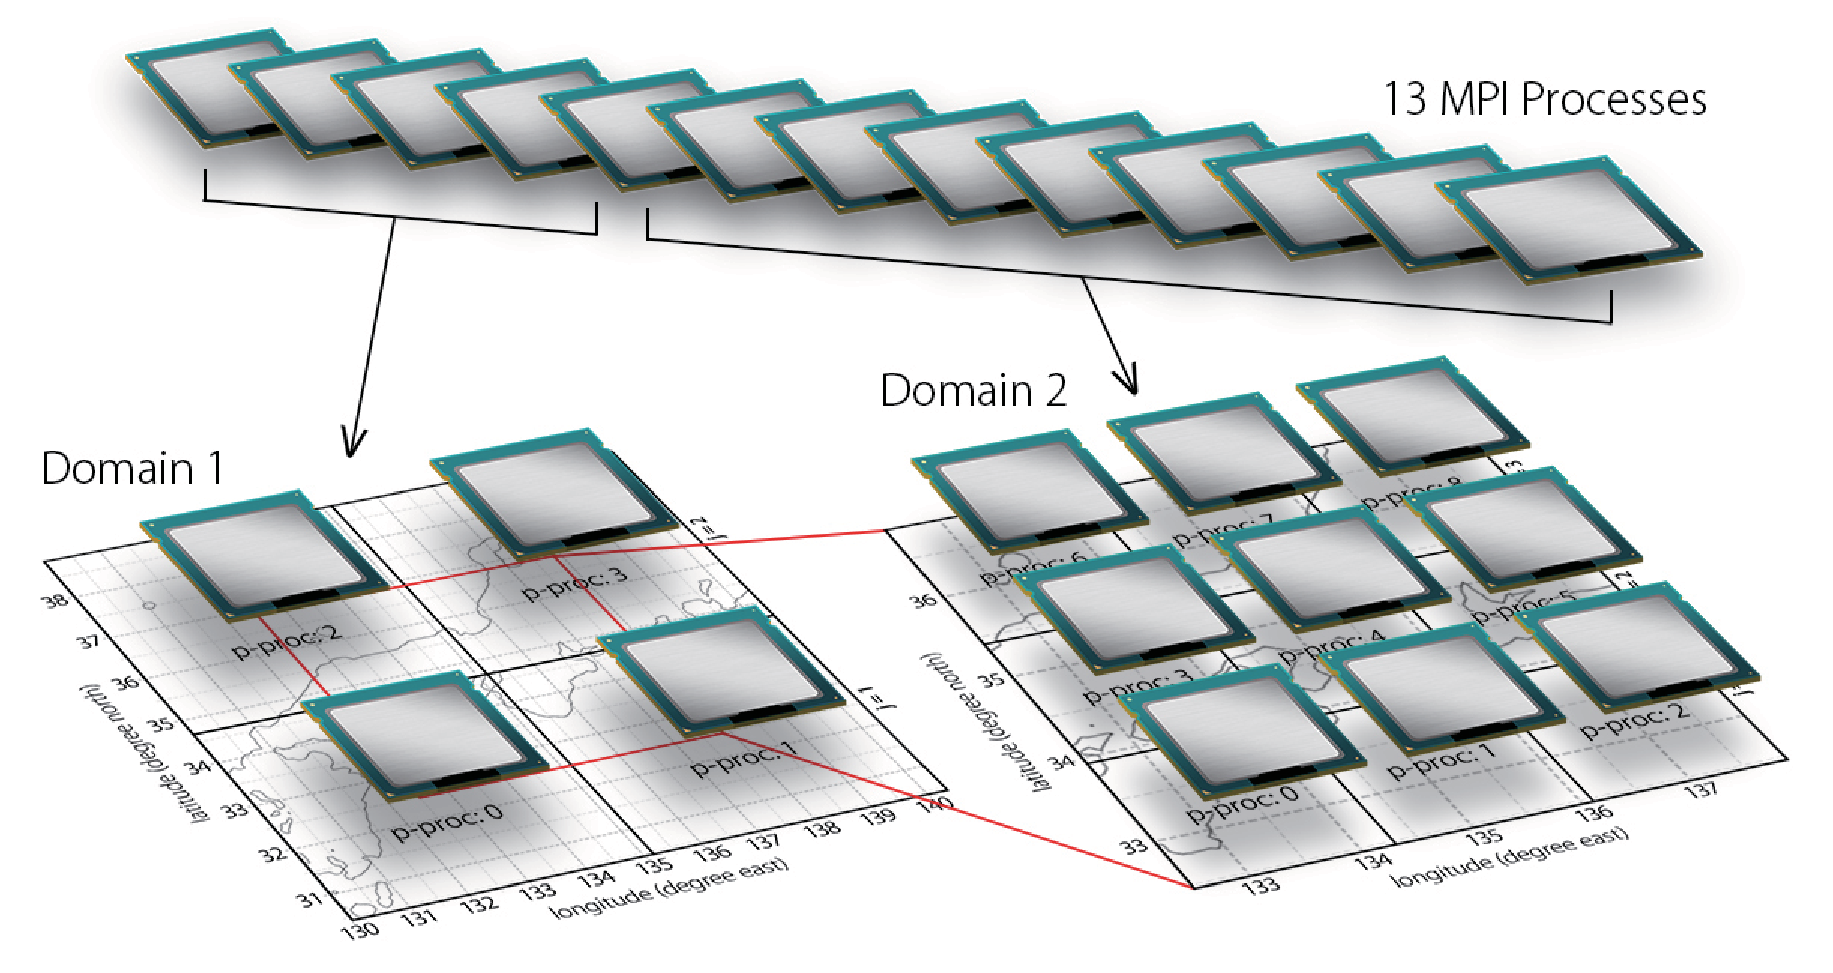
\includegraphics[width=0.8\hsize]{./figure/mpisplit_nesting.eps}\\
  \caption{オンライン・ネスティング実験のMPIプロセス配分イメージ. 全部で13のプロセスを立ち上げ、これを適切に分配することで、
           Domain 1は$2 \times 2$の4-MPI並列、Domain 2は$3 \times 3$の9-MPI並列計算を行う。Domain 1からDomain 2へMPI通信
           によってデータを受け渡ししながら時間積分計算を進める。}
  \label{fig_mpisplit}
\end{center}
\end{figure}




以下では、最も単純な2段ネスティングの例を示しながら、
オンライン・ネスティング実験のための設定について説明する。
%を行う場合は、\verb|scale-rm|のモデル本体実行前に全ての領域について、
%地形/土地利用データの作成、及び初期値/境界値データの作成を事前に行っておく必要がある。
%従って、親領域と子領域それぞれについて、
%\verb|pp.***.conf|、\verb|init.***.conf|、そして\verb|run.***.conf|ファイルを事前に作成し、
ここで説明するオンライン・ネスティング実験の設定を記述した設定ファイルは、サンプル設定ファイル
\verb|${Tutorial_dir}/real/sample/USER.online-nesting.sh|を
USER.shに置き換えて、実験セット準備ツールを実行した場合に作成される。
説明を読み進める上で参考にしてもらいたい。
また、すでに、親領域、子領域ともに地形/土地利用データの作成、
及び初期値/境界値データの作成を終えているものとして説明を進める。
それぞれの領域の地形データの作成手順は、第\ref{subsec:nest_topo}節に示したとおりであり、
初期値/境界値データの作成は、通常計算(シングル領域計算)の場合と同じである。


\subsubsection{設定ファイルの編集}
まず、親領域と子領域のそれぞれの設定ファイル(\verb|run.***.conf|)において、
オンライン・ネスティングのための設定を追加する。
\namelist{PARAM_NEST}は、ネスティング実験のための設定項目である。\\

\noindent {\gt \verb|run.d01.conf|の編集内容}\\
{\small {\gt
\ovalbox{
\begin{tabularx}{145mm}{lX}
\verb|&PARAM_NEST|                          & \\
\verb| USE_NESTING              = .true., | & オンラインネスティング時には、\verb|.true.|とする\\
\verb| OFFLINE                  = .false.,| & オンラインネスティング時には、\verb|.false.|とする\\
\verb| ONLINE_DOMAIN_NUM        = 1,      | & 領域の番号。外側から1番。\\
\verb| ONLINE_IAM_PARENT        = .true., | & \\
\verb| ONLINE_IAM_DAUGHTER      = .false.,| & \\
\verb| ONLINE_BOUNDARY_USE_QHYD = .true., | & \\
\verb| ONLINE_AGGRESSIVE_COMM   = .true., | & \\
\verb|/| \\
\end{tabularx}
}}}\\

\vspace{0.5cm}

\noindent {\gt \verb|run.d02.conf|の編集内容}\\
{\small {\gt
\ovalbox{
\begin{tabularx}{145mm}{lX}
\verb|&PARAM_NEST| & \\
\verb| USE_NESTING              = .true., | & オンラインネスティング時には、\verb|.true.|とする\\
\verb| OFFLINE                  = .false.,| & オンラインネスティング時には、\verb|.false.|とする\\
\verb| ONLINE_DOMAIN_NUM        = 2,      | & 領域の番号。外側から1番。\\
\verb| ONLINE_IAM_PARENT        = .false.,| & \\
\verb| ONLINE_IAM_DAUGHTER      = .true., | & \\
\verb| ONLINE_BOUNDARY_USE_QHYD = .true., | & \\
\verb| ONLINE_AGGRESSIVE_COMM   = .true., | & \\
\verb|/| \\
\end{tabularx}
}}}\\

\noindent 
\nmitem{USE_NESTING = .true., OFFLINE = .false.}によって、
オンライン・ネスティング実験であることが決定される。
\nmitem{ONLINE_**}で始まる設定変数はオンライン・ネスティング実験
専用の設定変数である。\nmitem{ONLINE_DOMAIN_NUM}は、
領域のID番号であり、外側領域から内側領域へ順番に番号を振っていく。
ここでは、親領域は1番、子領域は2番と設定する。
\nmitem{ONLINE_IAM_PARENT}と\nmitem{ONLINE_IAM_DAUGHTER}は、各領域が複数のネスティング領域の中でどこに位置するかを示している。
namelistの名前から明らかなように、
\verb|ONLINE_IAM_PARENT=.true.|であれば、子領域にデータを受け渡し、
\verb|ONLINE_IAM_DAUGHTER=.true.|であれば、境界値データは親領域から受け取るようになる。
%これらの変数は、``In online nesting system, I am parent (or, I am child).''という意味で覚えれば設定を間違うことはない。
N段ネスティング実験の場合の設定例を表\ref{tab:triple_nested}に示す。

\begin{table}[htb]
\begin{center}
\caption{N段ネスティング実験の設定例}
\begin{tabularx}{145mm}{|l|l|l|X|} \hline
 \rowcolor[gray]{0.9} 領域 & \verb|ONLINE_DOMAIN_NUM| & \verb|ONLINE_IAM_PARENT| & \verb|ONLINE_IAM_CHILD|\\ \hline
 最外領域 & 1               & .true.  & .false. \\ \hline
 中間領域 & 2\verb|〜|(N-1) & .true.  & .true. \\ \hline
 最内領域 & N               & .false. & .true. \\ \hline
\end{tabularx}
\label{tab:triple_nested}
\end{center}
\end{table}

\noindent 最外領域は親領域としてのみ働き、最内領域は子領域としてのみ働く。
一方、中間領域は最外領域に対しては子領域、
最内領域に対しては親領域として働くため両方共\verb|.true.|となる。
\nmitem{ONLINE_BOUNDARY_USE_QHYD}は、
「側面境界条件として親領域の凝結物の混合比を使うかどうか」を指定する。
外部入力データから側面境界条件を作成するときには通常使わないが、
ネスティングの場合、領域間の物理スキームの違いがなかったり、解像度もそれほど大きく離れていないため、
親領域で計算した凝結物を子領域の境界条件として与えることが可能である。
流入境界付近での雲や降水の生成の遅れの影響を小さくすることが期待される。



\subsubsection{launchファイルの編集}
\label{subsubsec:launch}
オンライン・ネスティング実験の実行には、
\verb|run.***.conf|の他に、起動用設定ファイル\verb|launch.conf|が必要である。\\

\noindent {\small {\gt
\ovalbox{
\begin{tabularx}{140mm}{lX}
\verb|&PARAM_LAUNCHER|      & \\
\verb| NUM_DOMAIN  = 2,|    & 領域の数\\
\verb| PRC_DOMAINS = 4, 16,| & それぞれの領域で使用するMPIプロセス数 (領域の数だけ必要)\\
\verb| CONF_FILES  = run.d01.conf, run.d02.conf,| & それぞれの領域の設定ファイル (領域の数だけ必要)\\
\verb|/|& \\
\end{tabularx}
}}}\\

\noindent 
\nmitem{PRC_DOMAINS}と\nmitem{CONF_FILES}の記載順は対応している必要がある。
上記の例の場合、親領域は4-MPI並列、子領域は16-MPI並列で実行するように指定されている。
ここで指定するMPIプロセス数は、各々の領域の設定ファイル (\verb|run.***.conf|) で指定されている
総MPIプロセス数(\verb|PRC_NUM_X|$\times$\verb|PRC_NUM_Y|)と一致させなければならない。

実行時には、シングル領域計算とは異なり、\verb|launch.conf|を引数に指定し、計算全体で使用するMPIプロセス数を指定して実行する。例えば、上記の例だとプロセス数は20となる。
\begin{verbatim}
 $ mpirun  -n  [プロセス数]  ./scale-rm  launch.conf
\end{verbatim}

実行にあたって注意することは、複数の領域の計算を同時に実行するため、
出力ファイル(\verb|historyファイル, LOGファイル, restartファイル|など) の書き出し先が重複しないように設定する必要がある。
例えば、\verb|historyファイル|は\verb|history_d01.pe***.nc, history_d02.pe***.nc|といったように
領域毎にファイル名を変えることで、どの領域の出力データであるか判別がつくように指定する。
出力ファイルのほか、入力ファイルである\verb|topoファイル, landuseファイル, boundaryファイル, initファイル|
の名前も注意が必要である。

実行時に次のようなエラーメッセージが出力されて計算が異常終了することがある。
これは、子領域で設定された計算領域が親領域の計算領域よりも大きいことを意味するエラーメッセージである。
``SW search''のエラーが出る場合は子領域の西側か南側が親領域の外側に出ており、``NE search''のエラーが出る場合は
子領域の東側か北側が親領域の外側に出ていることを意味している。再度設定を確認し、地形・土地利用データ、および
初期値/境界値作成からやり直すこと。\\


\noindent {\small {\gt
\fbox{
\begin{tabularx}{140mm}{l}
\verb|xxx region of daughter domain is larger than that of parent: SW search| \\
\end{tabularx}
}}}\\

\noindent {\small {\gt
\fbox{
\begin{tabularx}{140mm}{l}
\verb|xxx region of daughter domain is larger than that of parent: NE search| \\
\end{tabularx}
}}}\\



\subsubsection{MPIプロセスの分配ガイドライン}
%-------------------------------------------------------------------------
オンライン・ネスティング実験は、図\ref{fig_mpisplit}に示した通り、複数の領域間でMPIプロセスを共有しない。
つまり、それぞれのMPIプロセスは、どれか1つのネスティング領域の一部を担当することになる。
このため、ユーザーは、使用可能なMPIプロセス数のうち、各領域の計算にいくつのMPIプロセスを割り当てるかを
決める必要がある。割り当て配分のバランスが悪いと、待ち時間が発生し、計算時間が余計にかかってしまう。
これを避けるためには、領域毎に、時間積分にかかる1プロセスあたりの計算量(ここでは格子数と
タイムステップ数の積として定義)を揃えればよい
\footnote{正確を期すなら演算量を見積もる必要がある。}。
具体的な見積もり方法は下記の通りである。

ここではN個の領域(N段ネスティング)を考える。
n番目の領域の{\XDIR}, {\YDIR}, {\ZDIR}の格子数をそれぞれ\verb|IMAX_n|, \verb|JMAX_n|, \verb|KMAX_n|
と表し、時間積分のタイムステップ\nmitem{TIME_DT}を\verb|DT_n|と表すことにする。
この時、一番外側領域(n=1)の時間積分のタイムステップ\verb|DT_1|を基準とし、この時間を積分するのに
必要なn番目の領域の計算ステップ数は、
\begin{eqnarray}
 \verb|TSTEP_n| = \verb|DT_1| / \verb|DT_n|  \nonumber
\end{eqnarray}
と表される。領域全体での計算量は、領域が持つ格子数を掛けて
\begin{eqnarray}
 \verb|OPR_n| = \verb|IMAX_n| \times \verb|JMAX_n| \times \verb|KMAX_n| \times \verb|TSTEP_n| \nonumber
\end{eqnarray}
と見積もられる。n番目の領域に配分するMPIプロセス数の目安は、全MPIプロセス数を \verb|MPI_total|として
\begin{eqnarray}
 \verb|MPI_total| \times \frac{ \texttt{OPR\_n} }{ \sum_{m=1}^N \texttt{OPR\_m} }
\end{eqnarray}
と見積もることができる。


%ここでは、以下に示す2段オンライン・ネスティング実験を行う場合を想定し、ガイドラインに沿ったプロセス分配方法の例を示す。
%``domain 1''は外側の親領域、``domain 2''は内側の子領域を意味する。
%
%\begin{table}[htb]
%\begin{center}
%\caption{2段オンライン・ネスティング実験の設定想定}
%\begin{tabularx}{150mm}{|l|l|X|} \hline
% \rowcolor[gray]{0.9} 設定項目 & domain 1 & domain 2 \\ \hline
% 計算領域 & 450 km $\times$ 450 km & 200 km $\times$ 200 km \\ \hline
% DX \& DY(X,Y同一設定) & 3 km & 1 km \\ \hline
% 鉛直層設定 & 40層 & 60層 \\ \hline
% 積分時間間隔(DT)& 30 sec & 10 sec \\ \hline
% 積分時間 & 3600 sec & 3600 sec \\ \hline
%\end{tabularx}
%\label{tab:nest_proc_guide1}
%\end{center}
%\end{table}
%
%このとき、親領域の水平方向の一辺の格子点数は、$450 \mathrm{km} \div 3 \mathrm{km} = 150$点であるので、総格子点数は
%$X \times Y \times Z = 150 \times 150 \times 40 = 900,000$点である。一方、子領域の水平方向の一辺の格子点数は、
%$200 \mathrm{km} \div 1 \mathrm{km} = 200$点であるので、
%総格子点数は$200 \times 200 \times 60 = 2,400,000$点である。1つの時間ステップの
%積分を行うのにこれだけの格子点について計算を行わなければならない。
%
%積分時間間隔は格子間隔に依存するために領域毎に異なる。この例では、domain 1は30 secだが、domain 2は10 secであり、
%3倍の差がある。したがって、同じ30 secという積分時間に対してdomain 2は3倍多くの時間ステップ、つまり3倍の演算量を要する。
%これらを考慮して、簡単な領域間の演算量比率(Computation Rate)の指標を考えると下記の式で表される。
%\begin{eqnarray}
%ComputationRate=\frac{Xgrd_{child} \times Ygrd_{child} \times Zgrd_{child} \times Ustep_{child}}
%                     {Xgrd_{parent} \times Ygrd_{parent} \times Zgrd_{parent} \times Ustep_{parent}} \nonumber
%\end{eqnarray}
%ここで、$Xgrd, Ygrd, Zgrd$ はそれぞれ{\XDIR} 、{\YDIR}、{\ZDIR}の格子点数を表し、Ustepは単位時間積分に必要な時間ステップ数を表す。
%ここでの例をこの式に当てはまると、
%演算量比率は$(2,400,000 \times 3) \div (900,000 \times 1) = 8$であることがわかる。
%おおよそ、この割合にしたがってMPIプロセスを領域毎に分配すればよい。
%例えばdomain 1は4プロセス、domain 2は32プロセスを
%使用し、全体で36プロセスを使用する設定が考えられる。
%この場合、例えば次のように設定することができる。

%\begin{table}[htb]
%\begin{center}
%\caption{2段オンライン・ネスティング実験のMPIプロセス設定例}
%\begin{tabularx}{150mm}{|l|l|X|} \hline
% \rowcolor[gray]{0.9} 設定項目 & domain 1 & domain 2 \\ \hline
% MPIプロセス(X $\times$ Y) & 2 $\times$ 2 & 4 $\times$ 8 \\ \hline
% 水平格子点数(IMAX $\times$ JMAX) & 75 $\times$ 75 & 50 $\times$ 25 \\ \hline
%\end{tabularx}
%\label{tab:nest_proc_guide2}
%\end{center}
%\end{table}

{\XDIR} と{\YDIR}に分配するプロセス数\nmitem{PRC_NUM_X, PRC_NUM_Y}には任意性が残るが、
\verb|IMAX|と\verb|JMAX|の違いが小さくなるように設定する方がHALO領域を少なくすることが出来るため、
計算機の演算性能を引き出しやすいと考えられる\footnote{ただし、京の場合のようにスレッド並列も併用するハイブリッド並列の場合には{\YDIR}の格子点数をある程度大きくしてスレッド間の演算量のインバランスを小さくする必要性も出てくる。}。


以上の説明では、格子点数と積分時間のタイムステップだけを考慮して演算量比率を考えたが、
実際の計算では、物理過程の計算時間間隔も領域毎に異なる可能性があり、
領域内通信や領域間通信のMPI通信にかかる時間の違いも計算時間に影響を及ぼす。
オンライン・ネスティングの設定では、
最も計算負荷が高い領域(通常は最内領域)でMPI通信のための待ち時間が最小となるように
プロセスを分配するのが効率的であることが多い。
大規模計算や長期積分、繰り返し行うような実験の場合には、
上記の方法で効率的な配分を見積もり、いくらかの微調整を行うことを勧める。



 %完了

 \chapter{力学コアの設定}
 \section{Dynamical Core for Cartesian C-grid} \label{sec:atmos_dyn_cartesC}
%------------------------------------------------------
In this section, the dynamical core for the Cartesian C-grid is described.
The Cartesian C-grid is employed in \scalerm.
In the Cartesian C-grid, scalar quantities, such as density, thermodynamics variable and vapor, is defined at the cell center, while components of vector quantities, such as the momentums and fluxes, are defined at staggered point.
See the description document of \scalerm for more details.



\subsection{Setting Integration Numerical Method}  %\label{subsec:atmos_dyn_sover}
%------------------------------------------------------
The numerical method for time integration in the dynamical process is specified in \nmitem{ATMOS_DYN_TYPE} in \namelist{PARAM_ATMOS} in the configuration file.
\editboxtwo{
\verb|&PARAM_ATMOS  | & \\
\verb| ATMOS_DYN_TYPE    = "HEVE", | & ; Choose from Table \ref{tab:nml_dyn}.\\
\verb|/             | & \\
}

Time step depends on the sound speed in the case of using the explicit method, while it does not in the case of using the implicit method.
In most real atmospheric simulations, vertical grid spacing is much smaller than the horizontal ones.
Thus, fully explicit scheme, that is ``HEVE'', requires a quite small time step, which depends on vertical grid spacing and sound speed.
Therefore, ``HEVI'' is often used for the real atmospheric simulations.



\begin{table}[bth]
\begin{center}
  \caption{Options of methods for time integration in dynamical process}
  \label{tab:nml_dyn}
  \begin{tabularx}{150mm}{llX} \hline
    \rowcolor[gray]{0.9}  Scheme name & Description of scheme & Note\\ \hline
      \verb|HEVE|  & Fully explicit method & \\
      \verb|HEVI|  & Horizontally explicit and vertically implicit methods & Recommended for real experiment\\
    \hline
  \end{tabularx}
\end{center}
\end{table}


\subsection{Setting Temporal and Spatial Schemes} \label{subsec:atmos_dyn_scheme}
%------------------------------------------------------

The temporal and spatial schemes are configured in \namelist{PARAM_ATMOS_DYN}.
An example of setting, which is recommended for real atmospheric simulations,
is shown below.
\editboxtwo{
 \verb|&PARAM_ATMOS_DYN  | & \\
 \verb|ATMOS_DYN_TINTEG_SHORT_TYPE          = RK4,|          & ; Choose from temporal schemes in Table \ref{tab:nml_atm_dyn}\\
 \verb|ATMOS_DYN_TINTEG_TRACER_TYPE         = RK3WS2002,|    & ; Choose from temporal schemes\\
 \verb|ATMOS_DYN_FVM_FLUX_TYPE              = UD3,|          & ; Choose from temporal spatial schemes in Table \ref{tab:nml_atm_dyn}\\
 \verb|ATMOS_DYN_FVM_FLUX_TRACER_TYPE       = UD3KOREN1993,| & ; Choose from spatial schemes\\
 \verb|ATMOS_DYN_FLAG_FCT_TRACER            = .false.,|      & ; Use FCT scheme (.true.) or not (.false.)\\
 \verb|ATMOS_DYN_NUMERICAL_DIFF_COEF        = 0.D0, |        & \\
 \verb|ATMOS_DYN_NUMERICAL_DIFF_COEF_TRACER = 0.D0, |        & \\
 \verb|ATMOS_DYN_wdamp_height               = 15.D3,|        & ; height [m] of the bottom of sponge layer (for Rayleigh damping)\\
\verb|/             | & \\
}

The other options for temporal and spatial schemes are shown in Table \ref{tab:nml_atm_dyn}.
Note that the time step should be set according to the used schemes in order to ensure numerical stability.
An criteria to determine the time step is described in Section \ref{sec:timeintiv}.


\begin{table}[bth]
\begin{center}
  \caption{Setting temporal and spatial schemes}
  \label{tab:nml_atm_dyn}
  \begin{tabularx}{150mm}{lllX} \hline
    \rowcolor[gray]{0.9} & \multicolumn{1}{l}{Scheme name} & \multicolumn{1}{l}{Description of scheme} & \\ \hline
    \multicolumn{3}{l}{Temporal scheme} &  \\ \hline
    & \multicolumn{1}{l}{\verb|RK3|}       & \multicolumn{2}{l}{Heun-type 3 stage and 3rd-order Runge--Kutta scheme} \\
    & \multicolumn{1}{l}{\verb|RK3WS2002|} & \multicolumn{2}{l}{3 stage and generraly 2nd-order Runge--Kutta scheme in \citet{Wicker_2002}} \\
    & \multicolumn{1}{l}{\verb|RK4|}       & \multicolumn{2}{l}{4 stage and 4th-order Runge--Kutta scheme} \\
    & \multicolumn{1}{l}{\verb|RK7s6o|}    & \multicolumn{2}{l}{7 stage and 6th-order Runge--Kutta scheme in Lawson (1967) (supported only for HEVE)} \\
    & \multicolumn{1}{l}{\verb|RK11s8o|}   & \multicolumn{2}{l}{11 stage and 8th-order Runge--Kutta scheme in Cooper and Verner (1972)} \\
    & \multicolumn{1}{l}{}                 & \multicolumn{2}{l}{~~~~~(supported only for HEVE)} \\
    \hline
    \multicolumn{3}{l}{Spatial scheme} & \multicolumn{1}{l}{Minimum number of halos}\\ \hline
    & \multicolumn{1}{l}{\verb|CD2|} & \multicolumn{1}{l}{2nd-order central flux} & \multicolumn{1}{l}{1}\\
    & \multicolumn{1}{l}{\verb|CD4|} & \multicolumn{1}{l}{4th-order central flux} & \multicolumn{1}{l}{2}\\
    & \multicolumn{1}{l}{\verb|CD6|} & \multicolumn{1}{l}{6th-order central flux} & \multicolumn{1}{l}{3}\\
    & \multicolumn{1}{l}{\verb|CD8|} & \multicolumn{1}{l}{8th-order central flux} & \multicolumn{1}{l}{3}\\
    & \multicolumn{1}{l}{\verb|UD3|} & \multicolumn{1}{l}{3rd-order upwind flux} & \multicolumn{1}{l}{2}\\
    & \multicolumn{1}{l}{\verb|UD5|} & \multicolumn{1}{l}{5th-order upwind flux} & \multicolumn{1}{l}{3}\\
    & \multicolumn{1}{l}{\verb|UD7|} & \multicolumn{1}{l}{7th-order upwind flux} & \multicolumn{1}{l}{3}\\
    & \multicolumn{1}{l}{\verb|UD3KOREN1993|} & \multicolumn{1}{l}{3rd-order upwind flux + \citet{Koren_1993}'s filter} & \multicolumn{1}{l}{2}\\
\hline
  \end{tabularx}
\end{center}
\end{table}

The default setting for advection scheme used for the prognostic variables in dynamics, spcified by \nmitem{ATMOS_DYN_FVM_FLUX_TYPE}),
is the 4th-order central flux (\verb|CD4|) in the \scalerm.
When using \verb|CD4| in a simulation with a steep terrain,
an artificial grid-scale vertical flow is often seen at the peak of mountains.
This grid-scale flow may be reduced by using \verb|UD3|.
So, the use of \verb|UD3| is recommended for experiments with steep terrains.


\subsection{Numerical Diffusions} \label{subsec:numdiff}

The numerical stability depends on schemes for the dynamical process used in simulations (Sec. \ref{subsec:atmos_dyn_scheme}).
The stability would be improved by applying numerical diffusion.
\scalerm has the hyper-diffusion and divergence dumping as the explicit numerical diffusion.

The setting for them is the following:
\editboxtwo{
 \verb|&PARAM_ATMOS_DYN  | & \\
 \verb|ATMOS_DYN_NUMERICAL_DIFF_LAPLACIAN_NUM = 2,    |        & \\
 \verb|ATMOS_DYN_NUMERICAL_DIFF_COEF          = 1.D-4,|        & \\
 \verb|ATMOS_DYN_NUMERICAL_DIFF_COEF_TRACER   = 0.D0, |        & \\
 \verb|ATMOS_DYN_DIVDMP_COEF                  = 0.D0, |        & \\
\verb|/                  | & \\
}

The hyper-diffusion reduces the high frequency component of a target variable; it is mainly used to remove numerical noise.
The hyper-diffusion of a variable $\phi$ is defined as
\begin{equation}
  \nu \Delta^n \rho ( \phi - \phi_0 ),
\end{equation}
where $\nu$ is diffusion coefficient, $\phi_0$ is the reference state (See Section \ref{subsec:refstat}), and $\Delta$ is the Laplacian operator,
\begin{equation}
  \Delta^n = \nabla^{2n} = \frac{\partial^{2n}}{\partial x^{2n}} + \frac{\partial^{2n}}{\partial y^{2n}} + \frac{\partial^{2n}}{\partial z^{2n}}.
\end{equation}
The order of the Laplacian operator is specified by \\
\nmitem{ATMOS_DYN_NUMERICAL_DIFF_LAPLACIAN_NUM}. 
\nmitem{ATMOS_DYN_NUMERICAL_DIFF_COEF} and \\
\nmitem{ATMOS_DYN_NUMERICAL_DIFF_COEF_TRACER} is a non-dimensional coefficient of the hyper-diffusion.
\nmitem{ATMOS_DYN_NUMERICAL_DIFF_COEF} is a coefficient for the dynamical prognostic variables, such as density, momentum and potential temperature, \\
and \nmitem{ATMOS_DYN_NUMERICAL_DIFF_COEF_TRACER} is a coefficient for the tracer variables, such as specific humidity, hydrometeors, and turbulent kinetic energy.
The two-grid scale noise is dumped to $1/e$ in a one time step if the coefficient is unity.
The dumping is stronger for a larger coefficient.
The hyper-diffusion itself may cause numerical instability if the coefficient is larger than 1.
\nmitem{ATMOS_DYN_NUMERICAL_DIFF_COEF} can be set to zero when using the upwind schemes, such as \verb|UD3, UD5|, because they have implicit numerical diffusion.


The divergence dumping can also be available to improve numerical stability.
The divergence dumping reduces the three-dimensional divergence component; it is mainly used to remove sound waves.
Its coefficient can be set by \nmitem{ATMOS_DYN_DIVDMP_COEF}.


\subsection{Positive Definite}

For tracer advection, guaranteeing a non-negative value is required in most cases.\\
The \verb|UD3KOREN1993| scheme guarantees a non-negative value, whereas other schemes do not.
When schemes other than \verb|UD3KOREN1993| are used the FCT filter can be used to guarantee the non-negative value.
The advection scheme is specified by \nmitem{ATMOS_DYN_FVM_FLUX_TRACER_TYPE}, and switch for the FCT filter is \nmitem{ATMOS_DYN_FLAG_FCT_TRACER}$=$\verb|.true.|.


\subsection{Halos}

The necessary number of halos grid depends on the spatial difference scheme as shown in Table \ref{tab:nml_atm_dyn}.
Set \nmitem{IHALO} and \nmitem{JHALO} in \namelist{PARAM_ATMOS_GRID_CARTESC_INDEX} for the number of halos grid for the x- and y-directions, respectively.
By default, the number of the grid is 2, which is suitable for ``UD3'', ``UD3KOREN1993'', and ``CD4''.
For example, the configuration of the halo for the fifth-order upwind difference scheme is as follows:

\editboxtwo{
 \verb|&PARAM_ATMOS_GRID_CARTESC_INDEX | &  \\
 \verb| IHALO = 3,|   &\\
 \verb| JHALO = 3,|   &\\
 \verb|/ | & \\
}


\subsection{Setting for Coriolis Force} \label{subsec:coriolis}
%----------------------------------------------------------

In this subsection, treatments of the Coriolis force in \scalerm is explained.
The Coriolis parameter is zero as the default, so that you have to set (some) parameter(s) to introduce the Coriolis force in the simulation.
There are two types of setting for the Coriolis parameter: $f$-/$\beta$-plane and sphere.
The type can be specified by \nmitem{CORIOLIS_type} in \namelist{PARAM_CORIOLIS}.

\subsubsection{$f$-/$\beta$-plane}
If \nmitem{CORIOLIS_type} is set to ``PLANE'', the Coriolis parameter $f$ is $f=f_0 + \beta (y-y_0)$.
When $f_0=0$ and $\beta=0$, which is default, no Coriolis force is taken into account.

The plane for $\beta=0$ is called $f$-plane, otherwise it is called $\beta$-plane.
The parameters of $f_0, \beta$ and $y_0$ is set with the parameters of \namelist{PARAM_CORIOLIS} as follows:
\editbox{
  \verb|&PARAM_CORIOLIS| \\
  \verb| CORIOLIS_type = 'PLANE',| ! PLANE or SPHERE \\
  \verb| CORIOLIS_f0   = 1.0D-5, | ! $f_0$ \\
  \verb| CORIOLIS_beta = 0.0D0,  | ! $\beta$ \\
  \verb| CORIOLIS_y0   = 0.0D0,  | ! $y_0$ \\
  \verb|/| \\
}

The default values of the \nmitem{CORIOLIS_f0}, \nmitem{CORIOLIS_beta}, 
and \nmitem{CORIOLIS_y0} are 0.0, 0.0, and $y$ at the domain center, respectively.

If you want to add the geostrophic pressure gradient force that is in balance with the Coriolis force accompanied by the geostrophic wind, you need to modify the user specific file \verb|mod_user.f90| (see Section \ref{sec:mod_user}).
The test case of \verb|scale-rm/test/case/inertial_oscillation/20km| is an example of a simulation on the $f$-plane with the geostrophic pressure gradient force.


\subsubsection{Sphere}
On the sphere, the Coriolis parameter depends on the latitude as $f = 2\Omega \sin(\phi)$, where $\Omega$ and $\phi$ are angular velocity of the sphere and latitude, respectively.
In this case, you have to set \nmitem{CORIOLIS_type} = ``SPHERE''.
The angular velocity of the sphere is set by \nmitem{CONST_OHM} parameter of \namelist{PARAM_CONST} (see Section \ref{subsec:const}).
The latitude of the individual grids is determined depending on the map projection, which is explained in Section \ref{subsec:adv_mapproj}.



\subsubsection{Lateral Boundary Condition for Coriolis Force}

If there exists geostrophic wind, the periodic boundary conditions cannot be applied in its perpendicular direction, since the wind is not periodic.
For the $f$-plane, the double periodic boundary conditions can be applied with no geostrophic wind.
For the $\beta$-plane or sphere, the periodic boundary condition cannot be used in the y-direction, since the Coriolis parameter differs at the southern and northern boundaries.
In the absent of meridional geostrophic wind, the periodic boundary in the x-direction is allowed for the all the settings (i.e., the $f$-plane, $\beta$-plane, and sphere).


The nudge lateral boundary conditions at the south and north boundaries might be used for $f$- and $\beta$-plane experiment.
For the details of the nudging boundary, see Sections \ref{subsec:buffer}.
The test case of \verb|scale-rm/test/case/rossby_wave/beta-plane| is an example of a simulation on the $\beta$-plane with the south and north nudging boundaries.




\subsection{Setting for Reference State} \label{subsec:refstat}
%----------------------------------------------------------

As explained in Section \ref{subsec:numdiff}, the reference state is used in the calculation of numerical diffusion in the dynamical processes.
It is also used to calculate the pressure gradients in the momentum equations.
Since the reference state is defined under the hydrostatic balance, the deviation from the reference state can be used to calculate the pressure gradients.



The settings for the reference state are the following:
\editboxtwo{
 \verb|&PARAM_ATMOS_REFSTATE  | & \\
 \verb|ATMOS_REFSTATE_IN_BASENAME  = "",                 | & ! input file name \\
 \verb|ATMOS_REFSTATE_OUT_BASENAME = "",                 | & ! output file name \\
 \verb|ATMOS_REFSTATE_OUT_TITLE    = "SCALE-RM RefState, | & ! title in the output file \\
 \verb|ATMOS_REFSTATE_OUT_DTYPE    = "DEFAULT",          | & ! data type in the output file \\
 \verb|ATMOS_REFSTATE_TYPE         = "UNIFORM",          | & ! type of reference state \\
 \verb|ATMOS_REFSTATE_TEMP_SFC     = 300.0D0,            | & ! surface potential temperature \\
 \verb|ATMOS_REFSTATE_RH           = 0.0D0,              | & ! relative humidity \\
 \verb|ATMOS_REFSTATE_POTT_UNIFORM = 300.0D0,            | & ! potential temperature \\
 \verb|ATMOS_REFSTATE_UPDATE_DT    = -1.0D0,             | & ! update interval [sec] \\
\verb|/                                                  | & \\
}

If \nmitem{ATMOS_REFSTATE_IN_BASENAME} is specified, the reference state is read from the file.
Otherwise, the reference state is generated at the initial time of a simulation with the type specified by \nmitem{ATMOS_REFSTATE_TYPE}.
It can be \verb|"ISA"|, \verb|"UNIFORM"|, \verb|"ZERO"|, or \verb|"INIT"|:
\begin{description}
\item[ISA]
  The international standard atmosphere where the surface potential temperature, \\
  relative humidity, and the surface pressure are specified by \nmitem{ATMOS_REFSTATE_TEMP_SFC}, \nmitem{ATMOS_REFSTATE_RH}, and \nmitem{CONST_Pstd} (See Section \ref{subsec:const}), respectively.
\item[UNIFORM]
  The constant potential temperature and relative humidity profile specified \\
  by \nmitem{ATMOS_REFSTATE_POTT_UNIFORM} and \nmitem{ATMOS_REFSTATE_RH}, respectively.
\item[ZERO]
  The profile with all variables set to zero.
\item[INIT]
  The horizontally averaged initial state.
\end{description}

When \nmitem{ATMOS_REFSTATE_TYPE} is \verb|"INIT"|,
the reference state can be updated during the simulation.
The update interval is specified by \nmitem{ATMOS_REFSTATE_UPDATE_DT}. \\The unit of \nmitem{ATMOS_REFSTATE_UPDATE_DT} is seconds.
The updated reference state is the horizontally averaged value at the update time.
If \nmitem{ATMOS_REFSTATE_UPDATE_DT} is set to a negative value, the reference state is not updated during the simulation.


For a restart simulation, you need to pay attention to the setting of the reference state.
In order for the result of a restart simulation to be the same as that of the continuous simulation,
it is necessary to set so that the reference state of both are the same.
%
If you use an \verb|"INIT"|-type and update the reference state (\nmitem{ATMOS_REFSTATE_UPDATE_DT} $>$ 0),
the reference states of the two simulations will be identical
by setting the update interval (\nmitem{ATMOS_REFSTATE_UPDATE_DT}) to a divisor of the restart interval.
%
If you use an \verb|"INIT"|-type and do not update the reference state (\nmitem{ATMOS_REFSTATE_UPDATE_DT} $<$ 0),
you can use the same reference state by outputting the state to a file specified by \nmitem{ATMOS_REFSTATE_OUT_BASENAME} in the run before the restart and inputting the state from the file by specifying \nmitem{ATMOS_REFSTATE_IN_BASENAME} in the run after the restart.

 %完了
 %input \section{Dynamical core for \scalegm} here


 \chapter{物理過程の設定} \label{sec:basic_usel_physics}
 %\section{Setting the physical process} \label{sec:basic_usel_physics}
%------------------------------------------------------


\section{Cloud Micro-Physics} \label{sec:basic_usel_microphys}
%------------------------------------------------------
The cloud micro-physics scheme is configured in \nmitem{ATMOS_PHY_MP_TYPE} in \namelist{PARAM_ATMOS} in files \verb|init.conf| and \verb|run.conf|, respectively.
Note that it is necessary to specify the same scheme for \nmitem{ATMOS_PHY_MP_TYPE} in the configure files for both init and run executions.
The update interval for the cloud micro-physics scheme is specified in \namelist{PARAM_TIME}. Refer to Section \ref{sec:timeintiv} for the detailed configuration of calling timing.
The following example shows the configuration for cases involving a six-class one-moment bulk scheme that contains ice phase clouds:

\editboxtwo{
\verb|&PARAM_ATMOS  | & \\
\verb| ATMOS_PHY_MP_TYPE = "TOMITA08", | & ; Choose from Table \ref{tab:nml_atm_mp}.\\
\verb|/             | & \\
}

\begin{table}[tbh]
\begin{center}
  \caption{List of cloud micro-physics scheme types}
  \label{tab:nml_atm_mp}
  \begin{tabularx}{150mm}{lXX} \hline
    \rowcolor[gray]{0.9}  Schemes & Description of scheme & Reference\\ \hline
     \verb|OFF|      & Do not calculate phase change of water by cloud micro-physics. &  \\
     \verb|KESSLER|  & Three-class one-moment bulk scheme & \citet{kessler_1969} \\
     \verb|TOMITA08| & Six-class one-moment bulk scheme & \citet{tomita_2008} \\
     \verb|SN14|     & Six-class two-moment bulk scheme & \citet{sn_2014} \\
     \verb|SUZUKI10| & Spectral bin scheme (consideration of ice cloud can be specified as option) & \citet{suzuki_etal_2010} \\
%    \verb|XX|       & Super droplet scheme              & \citer{Shima_etal_2009} \\
    \hline
  \end{tabularx}
\end{center}
\end{table}

Four typical schemes are prepared:
\begin{enumerate}
\item {\bf One-moment bulk scheme without ice \cite{kessler_1969}}\\ This scheme assumes that the particle size distribution function is expressed only by mass concentration. Considering two categories of water in cloud and rain, the ratios of the densities of cloud and rain to total air density are prognostically predicted.
\item {\bf One-moment bulk scheme with ice \cite{tomita_2008}}\\
This scheme makes the same assumption as that in \cite{kessler_1969} for the particle size distribution function, but with five categories of water: cloud, rain, ice, snow, and graupel.
\item {\bf Two-moment bulk scheme with ice \cite{sn_2014}}\\
In this scheme, the particle size distribution is expressed by the numerical concentration of particles and their mass concentration.
\item {\bf One-moment bin scheme \cite{suzuki_etal_2010}}\\
This scheme explicitly expresses particle size distribution by discretizing it using an appropriate number of degrees of freedom for each category. There are six categories: cloud, rain, ice, snow, graupel, and hail. The accuracy of expressing the size distribution depends on the degrees of freedom.

\end{enumerate}
The degrees of sophistication increases from 1 to 4, as does computational cost.

If \verb|SUZUKI10| is selected, in addition to the specification of \nmitem{ATMOS_PHY_MP_TYPE}, the following configuration needs to be added to both configuration files of init and run executions:
\editboxtwo{
\verb|&PARAM_ATMOS_PHY_MP_SUZUKI10_bin|   &  \\
\verb| nbin   = 33, | & ; The number of bins \\
\verb| ICEFLG =  1, | & ; Option for consideration of ice cloud: 0(not considered), 1(considered) \\
\verb| kphase = 0, | & ; Type of collection kernel function for collision/coagulation processes: 0 is hydro-dynamic kernel, 1 is Golovin type kernel (\cite{golovin_1963}), and 2 is Long type kernel (\cite{long_1974}). Pleas see the description document of SCALE-RM for more details.  \\
\verb|/|            & \\
}
In this case, \namelist{PARAM_ATMOS_PHY_MP_SUZUKI10_bin} in the init configuration file must also be same as in the run configuration file. A necessary file \verb|micpara.dat| is automatically generated. If file \verb|micpara.dat| already exists, it is used for the calculation. When changing \verb|nbin| as described in the first line, this file is regenerated. If \verb|nbin| in file \verb|run.conf| is different from that in file \verb|micpara.dat|, the following error message is output and the simulation program is terminated instantaneously without calculation:
\msgbox{
\verb|ERROR [ATMOS_PHY_MP_suzuki10_setup] nbin in inc_tracer and nbin in micpara.dat is| \\
\verb|different check!| \\
}
To avoid this error, it is necessary to delete the old \verb|micpara.dat| beforehand and regenerate it. The regeneration is automatically done at the execution of \scalerm with \verb|SUZUKI10|.

 %完了
 \section{積雲パラメタリゼーション} \label{sec:basic_usel_cumulus}

積雲パラメタリゼーションは、設定ファイル\verb|init.conf|と\verb|run.conf|中の
\namelist{PARAM_ATMOS}の\nmitem{ATMOS_PHY_CP_TYPE}で指定する。
積雲パラメタリゼーションを呼び出す時間間隔は、\namelist{PARAM_TIME}で設定する
(詳細は第\ref{sec:timeintiv}節を参照)。

\editboxtwo{
\verb|&PARAM_ATMOS  | & \\
\verb| ATMOS_PHY_CP_TYPE = "KF", | & ; 表\ref{tab:nml_atm_cp}に示すスキームから選択 \\
\verb|/             | & \\
}
\begin{table}[h]
\begin{center}
  \caption{積雲パラメタリゼーションの選択肢}
  \label{tab:nml_atm_cp}
  \begin{tabularx}{150mm}{lXX} \hline
    \rowcolor[gray]{0.9}  スキーム名 & スキームの説明 & 参考文献 \\ \hline
      \verb|OFF|  & 積雲パラメタリゼーションを使用しない &  \\
      \verb|KF|   & Kain-Fritsch 対流パラメタリゼーション & \citet{kain_1990,kain_2004} \\
    \hline
  \end{tabularx}
\end{center}
\end{table}

\scalerm の現版では、積雲パラメタリゼーションとして\verb|KF|のみ対応している。
\verb|KF| は質量フラックス保存型の積雲パラメタリゼーションスキームであり、
サブグリッドスケールの一つの積雲を表現する。
格子間隔が 5 km 以下の場合に、非自然的な強力な深い対流が計算されることを避けるために、
この積雲パラメタリゼーションを使用することを推奨する。
積雲パラメタリゼーションと雲微物理のスキームは、
\verb|RAIN_CP|\verb|RAIN_MP|という名前で別々に降水量を出力する。
\verb|RAIN|と\verb|PREC|は、両者のスキームによる合計の降水量である。
つまり、\verb|RAIN| = \verb|RAIN_CP| + \verb|RAIN_MP|、
\verb|PREC| = \verb|PREC_CP| + \verb|PREC_MP|である。
%%%
\verb|KF|は大気中の水蒸気と水物質(雲水・雲氷等)の変化を計算することに注意が必要である。
水物質の変化は、雲微物理の過程でさらに計算される。
\verb|KF|では、雲水や雲氷等の数密度は考慮されない。
したがって、\verb|KF|における水物質の変化と関係した数密度の変化は、指定した関数によって見積もられ、2モーメントの雲微物理スキームへと渡される。

\subsubsection{\texttt{Kain-Fritsch}スキームに関する設定}

\verb|KF|では、以下のチューニングパラメータを設定できる。
\editboxtwo{
\verb|&PARAM_ATMOS_PHY_CP_KF  | & \\
\verb| ATMOS_PHY_CP_kf_trigger_type = 1,|     & ; トリガー関数の種類: 1=Kain, 3=Narita-Ohmori\\
\verb| ATMOS_PHY_CP_kf_dlcape      = 0.1,|   & ; CAPE の減率 \\
\verb| ATMOS_PHY_CP_kf_dlifetime   = 1800,|  & ; 深い対流の生存時間のスケール[sec]\\
\verb| ATMOS_PHY_CP_kf_slifetime   = 2400,|  & ; 浅い対流の生存時間のスケール[sec]\\
\verb| ATMOS_PHY_CP_kf_DEPTH_USL   =  300,|  & ; 上昇流の発生源となる層(updraft source layer)の探索開始時の深さ[hPa]\\
\verb| ATMOS_PHY_CP_kf_prec_type   = 1,|     & ; 降水の種類: 1=Ogura-Cho, 2=Kessler\\
\verb| ATMOS_PHY_CP_kf_rate        = 0.03, | & ; Ogura-Cho の降水関数における雲水と降水の比 \\
\verb| ATMOS_PHY_CP_kf_thres       = 1.E-3,| & ; Kessler の降水関数における Autoconversion の比 \\
\verb| ATMOS_PHY_CP_kf_LOG         = false,| & ; 警告メッセージを出力するか? \\
\verb|/             | & \\
}\\
ユーザーはトリガー関数として以下の2つから選択できる。
\begin{enumerate}
\item Kain タイプ \citet{kain_2004} \\
  \scalerm におけるデフォルト。
\item Narita and Ohmori タイプ \citet{narita_2007} \\
  日本域でより適していると思われるトリガー関数。
\end{enumerate}
また、 降水関数は以下の2つから選択できる。
\begin{enumerate}
\item Ogura-Cho タイプ \citet{ogura_1973} \\
  \scalerm におけるデフォルト。この場合、
  \nmitem{ATMOS_PHY_CP_kf_rate}というチューニングパラメータをさらに設定できる。
\item Kessler タイプ \citet{kessler_1969} \\
  Kessler type の簡単な降水関数。
  この場合、 \nmitem{ATMOS_PHY_CP_kf_thres}というチューニングパラメータをさらに設定できる。
\end{enumerate}

\namelist{PARAM_TIME}内の\nmitem{TIME_DT_ATMOS_PHY_CP}で指定する、
KF を呼び出す時間間隔もまたチューニングパラメータであり、降水量に影響を及す。
\nmitem{TIME_DT_ATMOS_PHY_CP}の最初の設定として 300 秒を推奨する。
\nmitem{PALAM_ATMOS_PHY_CP_kf_LOG}を\verb|true|にした場合は、
上昇流の発生源となる層がモデルの上下端を超えた際に警告メッセージを出力する。
上昇流の発生源となる層はしきい値(デフォルトでは 50 hPa)よりも厚い必要があるが、
この条件を満たさなくても計算は止まらない。
 %完了
 \section{\SubsecTurbulenceSetting} \label{sec:basic_usel_turbulence}
%------------------------------------------------------

Large-eddy シミュレーション(LES)において、
サブグリッドスケール乱流モデルは、
移流項によるサブグリッドスケールへのエネルギーカスケードを表現するためにある。

乱流スキームの選択は,init.confとrun.confにおける
\namelist{PARAM_ATMOS}内の\nmitem{ATMOS_PHY_TB_TYPE}で設定する。
乱流スキームを呼び出す時間間隔は、
\namelist{PARAM_TIME}で設定する(詳細は第\ref{sec:timeintiv}節を参照)。

\editboxtwo{
\verb|&PARAM_ATMOS  | & \\
\verb| ATMOS_PHY_TB_TYPE = "MYNN", | & ; 表\ref{tab:nml_atm_tb}より選択。\\
\verb|/             | & \\
}
\begin{table}[h]
\begin{center}
  \caption{乱流スキームの選択}
  \label{tab:nml_atm_tb}
  \begin{tabularx}{150mm}{lXX} \hline
    \rowcolor[gray]{0.9}  値 & スキームの説明 & 文献\\ \hline
      \verb|OFF|          & 乱流過程を計算しない &  \\
      \verb|SMAGORINSKY|  & Smagorinsky—Lilly 型のサブグリッドスケール乱流モデル & \citet{smagorinsky_1963,lilly_1962,Brown_etal_1994,Scotti_1993} \\
      \verb|D1980|        & Deardorff 型のサブグリッドスケール乱流モデル & \citet{Deardorff_1980} \\
    \hline
  \end{tabularx}
\end{center}
\end{table}

%SMAGORINSKY および D1980 は、ラージエディーシミュレーション(LES)用のサブグリッドスケール乱流モデルである。
%MYNN は、レイノルズ平均ナビエストークス方程式(RANS)計算用の境界層乱流パラメタリゼーションである。
%HYBRID は、LES と RANS 両者の乱流モデルを併用するものであり、以下の2通りの用途に用いられる。
%\begin{enumerate}
%\item LES と RANS の中間的な解像度 (グレーゾーン) での計算\\
%  各グリットの鉛直混合による時間変化率は、LES用乱流モデルとRANS用乱流パラメタリゼーションで得られた時間変化率を、実験解像度に応じた割合で線形的に足し合せることによって計算される。水平混合はLES用乱流モデルによって計算される。
%\item RANS計算における水平渦粘性\\
%  RANS計算における境界層乱流パラメタリゼーションは、鉛直にのみ混合を行い、水平方向には混合しない。HYBRID を指定し、以下の設定を追加することで、水平方向に渦粘性を導入することができる。この水平混合は、LES用の乱流モデルによって計算される。
%\end{enumerate}
\verb|SMAGORINSKY|スキームは、 RANS シミュレーションにおいて水平渦粘性としても使用できる。
惑星境界層パラメタリゼーション(第\ref{sec:basic_usel_pbl}節)は、
鉛直混合のみを取り扱うスキームである。
RANS シミュレーションにおいて水平粘性を考慮したければ、水平混合のために
サブグリッドスケール乱流モデルを使用されたい。
その場合は、以下のように\namelist{PARAM_ATMOS_PHY_TB_SMG}内の\nmitem{ATMOS_PHY_TB_SMG_horizontal}を\verb|.true.|にしなければならない。
\editboxtwo{
\verb|&PARAM_ATMOS_PHY_TB_SMG  | \\
\verb| ATMOS_PHY_TB_SMG_horizontal = .true., | \\
\verb|/             | \\
}
 %完了
 %Setting the physical process

\section{Planetary Boundary Layer Scheme} \label{sec:basic_usel_pbl}
%------------------------------------------------------

The planetary boundary layer (PBL) parameterization is a scheme for vertical mixing by turbulence in the PBL.
It is for Reynolds-Averaged Navier-Stokes equations (RANS) simulations.

The planetary boundary layer parameterization scheme is specified in \nmitem{ATMOS_PHY_BL_TYPE} in \namelist{PARAM_ATMOS} in files \verb|init.conf| and \verb|run.conf|. The timing of the calling of PBL scheme is specified in \namelist{PARAM_TIME}. Refer to Section \ref{sec:timeintiv} for the detailed configuration of the calling timing.

\editboxtwo{
\verb|&PARAM_ATMOS  | & \\
\verb| ATMOS_PHY_BL_TYPE = "MYNN", | & ; Select the scheme shown in Table \ref{tab:nml_atm_bl}\\
\verb|/             | & \\
}
\begin{table}[h]
\begin{center}
  \caption{List of planetary boundary layer scheme types}
  \label{tab:nml_atm_bl}
  \begin{tabularx}{150mm}{lXX} \hline
    \rowcolor[gray]{0.9}  Schemes & Description of scheme & Reference\\ \hline
      \verb|OFF|          & Do not calculate the PBL process &  \\
      \verb|MYNN|         & MYNN level 2.5 boundary scheme & \citet{my_1982,nakanishi_2004,nakanishi_2009} \\
    \hline
  \end{tabularx}
\end{center}
\end{table}

The PLB scheme calculate only vertical mixing.
If you want to consider the horizontal eddy viscosity in RANS simulations,
a sub-grid scale turbulence model can be used for the horizontal mixing.
See Section \ref{sec:basic_usel_turbulence} for the horizontal mixing.
 %完了
 \section{Radiation scheme} \label{sec:basic_usel_radiation}
%-------------------------------------------------------------------------------
The radiation scheme is specified in \nmitem{ATMOS_PHY_RD_TYPE} in \namelist{PARAM_ATMOS} in files \verb|init.conf| and \verb|run.conf|. The timing of the calling of the radiation scheme is specified in \namelist{PARAM_TIME}.  Refer to Section \ref{sec:timeintiv} for the detailed configuration of calling timing.

\editboxtwo{
\verb|&PARAM_ATMOS  | & \\
\verb| ATMOS_PHY_RD_TYPE = "MSTRNX", | & ; Select the radiation scheme shown in Table \ref{tab:nml_atm_rd}\\
\verb|/             | & \\
}\\

\begin{table}[h]
\begin{center}
  \caption{Choices of radiation scheme}
  \label{tab:nml_atm_rd}
  \begin{tabularx}{150mm}{lXX} \hline
    \rowcolor[gray]{0.9}  Value & Explanation of scheme & Reference\\ \hline
      \verb|OFF| or \verb|NONE| & Do not calculate the radiation scheme & \\
      \verb|OFFLINE|      & Use prescribed radiative data given from a file & \\
      \verb|MSTRNX|       & mstrnX (A k-distribution-based broadband radiation transfer model) & \citet{sekiguchi_2008} \\
%      \verb|WRF|          & mstrnX(Long wave) + Dudhia (shortwave) & \citet{dudhia_1989} \\
    \hline
  \end{tabularx}
\end{center}
\end{table}

\subsubsection{Configuration for \texttt{OFFLINE}}

When \nmitem{ATMOS_PHY_RD_TYPE} is \verb|OFFLINE| in \namelist{PARAM_ATMOS},
the file name and information of the data are specified in \namelist{PARAM_ATMOS_PHY_RD_OFFLINE}.

\editboxtwo{
\verb|&PARAM_ATMOS_PHY_RD_OFFLINE        | & \\
\verb| ATMOS_PHY_RD_OFFLINE_BASENAME              = "",          | & ; base name of external data file \\
\verb| ATMOS_PHY_RD_OFFLINE_AXISTYPE              = "XYZ",       | & ; order of spatial dimensions of the data. 'XYZ' or 'ZXY' \\
\verb| ATMOS_PHY_RD_OFFLINE_ENABLE_PERIODIC_YEAR  = .false.,     | & ; whether annually cyclic data \\
\verb| ATMOS_PHY_RD_OFFLINE_ENABLE_PERIODIC_MONTH = .false.,     | & ; whether monthly cyclic data \\
\verb| ATMOS_PHY_RD_OFFLINE_ENABLE_PERIODIC_DAY   = .false.,     | & ; whether daily cyclic data \\
\verb| ATMOS_PHY_RD_OFFLINE_STEP_FIXED            = 0,           | & ; step number when data at a certain time step is used. Set the value less than 1 for temporal varied data. \\
\verb| ATMOS_PHY_RD_OFFLINE_CHECK_COORDINATES     = .true.,      | & ; whether coordinate variables are to be checked \\
\verb| ATMOS_PHY_RD_OFFLINE_STEP_LIMIT            = 0,           | & ; maximum limit of steps. The data at the time step exceed this limit would not be read. 0 for no limit \\
\verb| ATMOS_PHY_RD_OFFLINE_DIFFUSE_RATE          = 0.5D0,       | & ; diffuse rate (diffuse solar radiation/global solar radiation) of short wave used when short-wave direct flux data is not given \\
\verb|/|            & \\
}

\noindent
The file format of external data file is \netcdf format
with the same coordinate variables as that of initial/boundary data files.
Variables required as the external data are shown in Table \ref{tab:var_list_atm_rd_offline}.\\

\begin{table}[h]
\begin{center}
  \caption{Radiative data as external file input}
  \label{tab:var_list_atm_rd_offline}
  \begin{tabularx}{150mm}{lXll} \hline
    \rowcolor[gray]{0.9}  Variable name & Description & \# of dimensions & \\ \hline
      \verb|RFLX_LW_up|     & Upward long-wave radiative flux & 3D (spatial) + 1D (time) \\
      \verb|RFLX_LW_dn|     & Downward long-wave radiative flux & 3D (spatial) + 1D (time) \\
      \verb|RFLX_SW_up|     & Upward short-wave radiative flux & 3D (spatial) + 1D (time) \\
      \verb|RFLX_SW_dn|     & Downward short-wave radiative flux & 3D (spatial) + 1D (time) \\
      \verb|SFLX_LW_up|     & Upward long-wave radiative flux at the surface & 2D (spatial) + 1D (time) \\
      \verb|SFLX_LW_dn|     & Downward long-wave radiative flux at the surface & 2D (spatial) + 1D (time) \\
      \verb|SFLX_SW_up|     & Upward short-wave radiative flux at the surface & 2D (spatial) + 1D (time) \\
      \verb|SFLX_SW_dn|     & Downward short-wave radiative flux at the surface & 2D (spatial) + 1D (time) \\
      \verb|SFLX_SW_dn_dir| & Downward short-wave direct radiative flux at the surface & 2D (spatial) + 1D (time) & optional \\
    \hline
  \end{tabularx}
\end{center}
\end{table}

\subsubsection{Configuration for \texttt{MSTRNX}}

The solar radiation is calculated by using date, time, longitude, and latitude according to the model configuration of calculation.
For the ideal experiment, they can be arbitrarily given as fixed values of time and location over the domain.
The solar constant can also be changed. These are configured in \namelist{PARAM_ATMOS_SOLARINS} as follows:

\editboxtwo{
\verb|&PARAM_ATMOS_SOLARINS                             | & \\
\verb| ATMOS_SOLARINS_constant     = 1360.250117        | & Solar constant [W/m2] \\
\verb| ATMOS_SOLARINS_set_ve       = .false.            | & Whether settings of the ideal vernal equinox are used \\
\verb| ATMOS_SOLARINS_set_ideal    = .false.            | & Whether values are fixed for obliquity and eccentricity \\
\verb| ATMOS_SOLARINS_obliquity    = 0.0                | & obliquity [deg.] in the case that \verb|ATMOS_SOLARINS_set_ideal=.true.| \\
\verb| ATMOS_SOLARINS_eccentricity = 0.0                | & eccentricity     in the case that \verb|ATMOS_SOLARINS_set_ideal=.true.| \\
\verb| ATMOS_SOLARINS_fixedlatlon  = .false.            | & Whether values are fixed for latitude and longitude at radiation calculation \\
\verb| ATMOS_SOLARINS_lon          = 135.221            | & Longitude [deg.] in the case that \verb|ATMOS_SOLARINS_fixedlatlon=.true.| \\
\verb| ATMOS_SOLARINS_lat          =  34.653            | & Latitude  [deg.] in the case that \verb|ATMOS_SOLARINS_fixedlatlon=.true.| \\
\verb| ATMOS_SOLARINS_fixeddate    = .false.            | & Whether values are fixed for date and time at radiation calculation \\
\verb| ATMOS_SOLARINS_date         = -1,-1,-1,-1,-1,-1, | & Date and time [Y,M,D,H,M,S] in the case that \verb|ATMOS_SOLARINS_fixeddate=.true.| \\
\verb|/                                                 | & \\
}\\

When \nmitem{ATMOS_SOLARINS_set_ideal} is \verb|.true.|,
the solar insolation is calculated using obliquity(deg.) and eccentricity
specified at \nmitem{ATMOS_SOLARINS_obliquity}, \\
\nmitem{ATMOS_SOLARINS_eccentricity}, respectively.
These configurations are useful for the ideal simulations and the simulations of planets other than the Earth.
%
When \nmitem{ATMOS_SOLARINS_fixedlatlon} is \verb|.true.|,
the solar insolation is calculated using same longitude and latitude
specified at \\
\nmitem{ATMOS_SOLARINS_lon, ATMOS_SOLARINS_lat} over the whole domain.
the default values of them are \nmitem{MAPPROJECTION_basepoint_lon, MAPPROJECTION_basepoint_lat},
which are set in \namelist{PARAM_MAPPROJECTION}.
Refer to Section \ref{subsec:adv_mapproj} for the explanation of \namelist{PARAM_MAPPROJECTION}.
%
When \nmitem{ATMOS_SOLARINS_fixeddate} is \verb|.true.|,
the solar insolation is calculated according to date and time (Y,M,D,H,M,S) specified at \nmitem{ATMOS_SOLARINS_date}.
The date and time are not fixed if the negative values are specified.
For example, when configuring \nmitem{ATMOS_SOLARINS_date} to \verb|1950,3,21,-1,-1,-1|,
The date is fixed to March 21, 1950 (the vernal equinox)
and diurnal variations of the solar insolation are considered in the simulation.
%
When \nmitem{ATMOS_SOLARINS_set_ve} is \verb|.true.|,
the multiple configurations of ideal vernal equinox is automatically set.
This option sets obliquity and eccentricity to zero, both longitude and latitude to zero deg., and the date and time to 12UTC, March 21, 1950.
If the values are specified by using \nmitem{ATMOS_SOLARINS_set_ideal, ATMOS_SOLARINS_fixedlatlon, ATMOS_SOLARINS_fixeddate} as described above,
those settings are given priority.

Depending on the experimental design, the top of the model is often too low, such as 10$\sim$ 20 km, compared to the height of the atmosphere.
To remedy this situation, another top height used only for radiation calculation is set.
The top height for radiation depends on the parameter file of the radiation scheme.
For example, when \verb|MSTRNX| is used, the default parameter table used for \verb|MSTRNX| assumes that it is 100 km.
%
For the calculation of radiation at levels higher than the top of the model, several layers are prepared.
The additional layers are 10 by default;
If the top of the model is 22 km, 10 additional layers with a grid spacing of 7.8 km are added for radiation calculation.
These are configured in \namelist{PARAM_ATMOS_PHY_RD_MSTRN}.\\

\verb|MSTRNX| requires a parameter table for radiation calculation.
By default, the wavelength between solar radiation and infrared radiation is divided into 29 bands/111 channels;
nine types of cloud and aerosol particles with eight particle bins are prepared in the table.
Three kinds of parameter files are prepared in the directory \verb|scale-rm/test/data/rad/|.

\begin{verbatim}
  scale-rm/test/data/rad/PARAG.29     ; absorption parameter for gas
  scale-rm/test/data/rad/PARAPC.29    ; absorption and scattering param. for particles
  scale-rm/test/data/rad/VARDATA.RM29 ; particle parameter for cloud and aerosol
\end{verbatim}
These files are specified in \namelist{PARAM_ATMOS_PHY_RD_MSTRN} as follows:

\editboxtwo{
\verb|&PARAM_ATMOS_PHY_RD_MSTRN | & \\
\verb| ATMOS_PHY_RD_MSTRN_KADD                  = 10             | & Number of layers between model top and TOA for radiation\\
\verb| ATMOS_PHY_RD_MSTRN_TOA                   = 100.0          | & Height of TOA for radiation [km] (depending on parameter file used)\\
\verb| ATMOS_PHY_RD_MSTRN_nband                 = 29             | & Number of bins for wavelength (depending on parameter file used)\\
\verb| ATMOS_PHY_RD_MSTRN_nptype                = 9              | & Number of aerosol species (depending on parameter file used)\\
\verb| ATMOS_PHY_RD_MSTRN_nradius               = 8              | & Number of particle bins for aerosol (depending on parameter file used)\\
\verb| ATMOS_PHY_RD_MSTRN_GASPARA_IN_FILENAME   = "PARAG.29"     | & Input file for absorption parameter by gas\\
\verb| ATMOS_PHY_RD_MSTRN_AEROPARA_IN_FILENAME  = "PARAPC.29"    | & Input file for absorption and scattering parameter by cloud and aerosol\\
\verb| ATMOS_PHY_RD_MSTRN_HYGROPARA_IN_FILENAME = "VARDATA.RM29" | & Input file for particle parameter of cloud and aerosol\\
\verb| ATMOS_PHY_RD_MSTRN_ONLY_QCI              = .false.        | & Whether only cloud water and ice are considered (rain, snow, graupel are ignored) \\
\verb|/| & \\
}\\

The parameter files were updated in version 5.2.
It is recommended to use new parameter files in the latest version of \scalerm.
The previous parameter files, provided in version 5.1 or earlier,
are located in the directory \verb|scale-rm/test/data/rad/OpenCLASTR|.
The number of particle type and the number of particle bins are different from those in the new parameter files.
So if you want to use these files, \nmitem{ATMOS_PHY_RD_MSTRN_nptype, ATMOS_PHY_RD_MSTRN_nradius} should be specified in \\
\namelist{PARAM_ATMOS_PHY_RD_MSTRN} as follows.

\editboxtwo{
\verb| ATMOS_PHY_RD_MSTRN_nptype = 11 |\\
\verb| ATMOS_PHY_RD_MSTRN_nradius = 6  |\\
}\\

It is necessary to provide vertical profiles of temperature, pressure, and gas concentration, such as carbon dioxide and ozone,
in additional layers for radiation calculation.
There are two methods for this. The profiles are input as climatologies or prepared by users in ASCII format. \\

In the case of providing climatologies, \scalerm provides the database form CIRA86\footnote{http://catalogue.ceda.ac.uk/uuid/4996e5b2f53ce0b1f2072adadaeda262} \citep{CSR_2006} for temperature and pressure,
and MIPAS2001 \citep{Remedios_2007} for gas species.
The climatology profiles are calculated from the databases according to date, time, latitude, and longitude.
If the fixed date and location are specified in \namelist{PARAM_ATMOS_SOLARINS}, the calculation of profile follows those settings.
The input files are also provided in the directory \verb|scale-rm/test/data/rad/|.
\begin{verbatim}
  scale-rm/test/data/rad/cira.nc       ; CIRA86 data (NetCDF format)
  scale-rm/test/data/rad/MIPAS/day.atm ; MIPAS2011 data for mid-lat. (ASCII format)
  scale-rm/test/data/rad/MIPAS/equ.atm ;   for tropics (ASCII format)
  scale-rm/test/data/rad/MIPAS/sum.atm ;   for summer-side high-lat. (ASCII format)
  scale-rm/test/data/rad/MIPAS/win.atm ;   for winter-side high-lat. (ASCII format)
\end{verbatim}
The file and directory names are specified in \namelist{PARAM_ATMOS_PHY_RD_PROFILE}.
The example of configuration of putting five files above to the current directory is as follows:

\editboxtwo{
\verb|&PARAM_ATMOS_PHY_RD_PROFILE | & \\
\verb| ATMOS_PHY_RD_PROFILE_use_climatology       = .true.    | & Whether climatologies of CIRA86 and MIPAS2001 are used \\
\verb| ATMOS_PHY_RD_PROFILE_CIRA86_IN_FILENAME    = "cira.nc" | & File name of \verb|CIRA86|\\
\verb| ATMOS_PHY_RD_PROFILE_MIPAS2001_IN_BASENAME = "."       | & Directory name which contains \verb|MIPAS2001| files\\
\verb|/| & \\
}\\

Gases considered in radiation calculation are water vapor($H_{2}O$), carbon dioxide($CO_{2}$), ozone($O_{3}$), Nauru's oxide($N_{2}O$), carbon monoxide($CO$), methane($CH_{4}$), oxigen($O_{2}$), and chlorofluorocarbons($CFCs$). These concentrations are able to be set to zero in \namelist{PARAM_ATMOS_PHY_RD_PROFILE}.

\editboxtwo{
\verb|&PARAM_ATMOS_PHY_RD_PROFILE | & \\
\verb| ATMOS_PHY_RD_PROFILE_USE_H2O = .true. | & When false, H2O concentration is zero.\\
\verb| ATMOS_PHY_RD_PROFILE_USE_CO2 = .true. | & When false, CO2 concentration is zero.\\
\verb| ATMOS_PHY_RD_PROFILE_USE_O3  = .true. | & When false, O3 concentration is zero.\\
\verb| ATMOS_PHY_RD_PROFILE_USE_N2O = .true. | & When false, N2O concentration is zero.\\
\verb| ATMOS_PHY_RD_PROFILE_USE_CO  = .true. | & When false, CO concentration is zero.\\
\verb| ATMOS_PHY_RD_PROFILE_USE_CH4 = .true. | & When false, CH4 concentration is zero.\\
\verb| ATMOS_PHY_RD_PROFILE_USE_O2  = .true. | & When false, O2 concentration is zero.\\
\verb| ATMOS_PHY_RD_PROFILE_USE_CFC = .true. | & When false, CFC concentration is zero.\\
\verb|/| & \\
}\\

In case of using user-defined profiles, users must prepare height [m], pressure [Pa], temperature [K], water vapor [kg/kg], and ozone concentration [kg/kg] in ASCII format. The concentrations of gases other than water vapor and ozone are set to zero, and temporal variation is not considered.
An example of user-defined files is provided in
\begin{verbatim}
  scale-rm/test/data/rad/rad_o3_profs.txt
\end{verbatim}
To use the user-defined profiles,
it is required to set \nmitem{ATMOS_PHY_RD_PROFILE_use_climatology} $=$ \verb|.false.| in \namelist{PARAM_ATMOS_PHY_RD_PROFILE},
and to specify the file and directory names in \nmitem{ATMOS_PHY_RD_PROFILE_USER_IN_FILENAME}.

\editboxtwo{
\verb|&PARAM_ATMOS_PHY_RD_PROFILE | & \\
\verb| ATMOS_PHY_RD_PROFILE_use_climatology  = .false. | & Whether climatologies of CIRA86 and MIPAS2001 are used \\
\verb| ATMOS_PHY_RD_PROFILE_USER_IN_FILENAME = ""      | & User-defined file in the case of not using climatorogies (ASCII format)\\
\verb|/| & \\
}\\

The number of layers and their heights in this user-defined file can be given independently of the default model configuration. During execution, the values in the model layers are interpolated from the given profiles. Note that if the top height considered TOA in the radiation calculation is higher than in the input profile, an extrapolation is adopted there.




 %完了
 \section{Surface Flux at the Bottom of Atmospheric Boundary } \label{sec:basic_usel_surface}
%------------------------------------------------------
The flux scheme at the bottom atmospheric boundary is configured in \nmitem{ATMOS_PHY_SF_TYPE} in \namelist{PARAM_ATMOS} as follows:

\editboxtwo{
\verb|&PARAM_ATMOS  | & \\
\verb| ATMOS_PHY_SF_TYPE = "COUPLE", | &  ; Select the surface flux scheme shown in Table \ref{tab:nml_atm_sf}\\
\verb|/             | & \\
}
If ocean, land, and urban models are not used, the bottom atmospheric boundary is assumed to be a virtual surface used in an ideal experiment. The timing of the calling of the surface flux scheme is configured in \namelist{PARAM_TIME}. Refer to Section \ref{sec:timeintiv} for the detailed configuration of the calling timing. If ocean, land, and urban models are used, ``COUPLE'' is given to \nmitem{ATMOS_PHY_SF_TYPE}:

\begin{table}[htb]
\begin{center}
  \caption{List for the atmospheric bottom boundary types}
  \label{tab:nml_atm_sf}
  \begin{tabularx}{150mm}{lX} \hline
    \rowcolor[gray]{0.9}  Schemes & Description of scheme\\ \hline
      \verb|NONE   | & Do not calculate surface flux, but \verb|"NONE"| is replaced to \verb|"COUPLE"| according to settings of ocean, land, and urban models) \\
      \verb|OFF    | & Do not calculate surface flux\\
      \verb|CONST  | & Fix the constant value of surface flux \\
      \verb|BULK   | & Calculate the surface flux in bulk model \\
      \verb|COUPLE | & Receive surface flux from ocean, land, and urban models \\
    \hline
  \end{tabularx}
\end{center}
\end{table}

%-------------------------------------------------------------------------------
\subsubsection{Configuration of Constant}

If \nmitem{ATMOS_PHY_SF_TYPE} $=$ \verb|"CONST"|, the surface flux can be kept to a value specified in \runconf as follows. The values below are the default ones.

\editboxtwo{
 \verb|&PARAM_ATMOS_PHY_SF_CONST                | & \\
 \verb| ATMOS_PHY_SF_FLG_MOM_FLUX   =    0      | & 0: Bulk coefficient is constant \\
                                                  & 1: Frictional velocity is constant  \\
 \verb| ATMOS_PHY_SF_U_minM         =    0.0E0  | & Lower limit of absolute velocity  [m/s] \\
 \verb| ATMOS_PHY_SF_Const_Cm       = 0.0011E0  | & Constant bulk coefficient for momentum \\
                                                  &  (Active at \verb|ATMOS_PHY_SF_FLG_MOM_FLUX = 0|) \\
 \verb| ATMOS_PHY_SF_CM_min         =    1.0E-5 | & Lower limit of bulk coefficient for momentum \\
                                                  &  (Active at \verb|ATMOS_PHY_SF_FLG_MOM_FLUX = 1|) \\
 \verb| ATMOS_PHY_SF_Const_Ustar    =   0.25E0  | & Constant fictional velocity [m/s] \\
                                                  &  (Active at \verb|ATMOS_PHY_SF_FLG_MOM_FLUX = 1|) \\
 \verb| ATMOS_PHY_SF_Const_SH       =    15.E0  | & Constant sensible heat flux at the surface [W/m2] \\
 \verb| ATMOS_PHY_SF_FLG_SH_DIURNAL =   .false. | & Whether diurnal variation is enabled for sensible heat flux [logical]\\
 \verb| ATMOS_PHY_SF_Const_FREQ     =    24.E0  | & Daily cycle if diurnal variation is enabled [hour]\\
 \verb| ATMOS_PHY_SF_Const_LH       =   115.E0  | & Constant latent heat flux at the surface [W/m2] \\
 \verb|/|            & \\
}

\subsubsection{Bulk Configuration}
%-------------------------------------------------------------------------------
If \nmitem{ATMOS_PHY_SF_TYPE} $=$ \verb|"BULK"|, the surface flux is calculated by the bulk model using the prescribed surface temperature and roughness lengths.
Evaporation efficiency can also be given optionally in a range of 0 to 1.
This flexibility enables the ideal experiment not only for ocean surfaces but also for land.
The evaporation efficiency is specified in \nmitem{ATMOS_PHY_SF_BULK_beta} in \namelist{PARAM_ATMOS_PHY_SF_BULK} in \runconf as follows:

\editboxtwo{
\verb|&PARAM_ATMOS_PHY_SF_BULK  | & \\
\verb| ATMOS_PHY_SF_BULK_beta = 1.0, | & ; Evaporation efficiency (the value must be in a range of 0 to 1). If this value is set as 0, the surface is assumed to be completely dry. If the value is 1, it is assumued to be completely wet (like ocean surface).\\
\verb|/             | & \\
}

The scheme for the bulk coefficient is configured in \nmitem{BULKFLUX_TYPE} in \namelist{PARAM_BULKFLUX} in the file \runconf as follows:

\editboxtwo{
\verb|&PARAM_BULKFLUX  | & \\
\verb| BULKFLUX_TYPE = "B91W01", | & ; Select the bulk coefficient scheme shown in Table \ref{tab:nml_bulk}\\
\verb|/                | & \\
}
\begin{table}[h]
\begin{center}
  \caption{List of bulk coefficient scheme types}
  \label{tab:nml_bulk}
  \begin{tabularx}{150mm}{llX} \hline
    \rowcolor[gray]{0.9}  Schemes & Description of scheme & Reference\\ \hline
      \verb|B91W01| & Bulk method by the universal function (Default) & \citet{beljaars_1991,wilson_2001} \\
      \verb|U95|    & Louis-type bulk method  (improved version of Louis (1979) & \citet{uno_1995} \\
    \hline
  \end{tabularx}
\end{center}
\end{table}
 %完了
 \section{Ocean model} \label{sec:basic_usel_ocean}
%-------------------------------------------------------------------------------
The ocean process consists of two main parts, i.e., update of sea surface state and flux calculation at the interface of atmosphere and ocean. The timing of calling these scheme is configured in \namelist{PARAM_TIME}. Refer to Section \ref{sec:timeintiv} for the detailed configuration of the calling timing.

\subsubsection{Sea surface scheme}
%-------------------------------------------------------------------------------
The manner of updating sea surface state, such as sea surface temperature, is configured in \nmitem{OCEAN_DYN_TYPE}, \nmitem{OCEAN_SFC_TYPE}, \nmitem{OCEAN_ALB_TYPE}, and \nmitem{OCEAN_RGN_TYPE} in \namelist{PARAM_OCEAN} in the files \verb|init.conf| and \verb|run.conf|:

\editboxtwo{
\verb|&PARAM_OCEAN           | & \\
\verb| OCEAN_DYN_TYPE = "SLAB", | & ; Select the sea dynamics type shown in Table \ref{tab:nml_ocean_dyn}\\
\verb| OCEAN_SFC_TYPE = "FIXED-TEMP", | & ; Select the sea surface type shown in Table \ref{tab:nml_ocean_sfc}\\
\verb| OCEAN_ALB_TYPE = "NAKAJIMA00", | & ; Select the sea albedo type shown in Table \ref{tab:nml_ocean_alb}\\
\verb| OCEAN_RGN_TYPE = "MOON07", | & ; Select the sea roughness type shown in Table \ref{tab:nml_ocean_rgn}\\
\verb|/                      | & \\
}
\begin{table}[h]
\begin{center}
  \caption{Choices of sea dynamics schemes}
  \label{tab:nml_ocean_dyn}
  \begin{tabularx}{150mm}{lX} \hline
    \rowcolor[gray]{0.9}  Values & Description of scheme \\ \hline
      \verb|NONE or OFF| & Not using the sea model \\
      \verb|SLAB|        & Slab ocean model \\
      \verb|INIT|        & Fixed as initial condition \\
    \hline
  \end{tabularx}
\end{center}
\end{table}

\begin{table}[h]
\begin{center}
  \caption{Choices of sea surface schemes}
  \label{tab:nml_ocean_sfc}
  \begin{tabularx}{150mm}{lX} \hline
    \rowcolor[gray]{0.9}  Values & Description of scheme \\ \hline
      \verb|FIXED-TEMP| & Do not update sea surface temperature \\
    \hline
  \end{tabularx}
\end{center}
\end{table}

\begin{table}[h]
\begin{center}
  \caption{Choices of sea albedo schemes}
  \label{tab:nml_ocean_alb}
  \begin{tabularx}{150mm}{llX} \hline
    \rowcolor[gray]{0.9}  Values & Description of scheme & reference \\ \hline
      \verb|NAKAJIMA00| & Sea albedo scheme & \citet{nakajima_2000} \\
      \verb|INIT|       & Fixed as initial condition \\
    \hline
  \end{tabularx}
\end{center}
\end{table}

\begin{table}[h]
\begin{center}
  \caption{Choices of sea roughness schemes}
  \label{tab:nml_ocean_rgn}
  \begin{tabularx}{150mm}{llX} \hline
    \rowcolor[gray]{0.9}  Values & Description of scheme & reference \\ \hline
      \verb|MOON07|   & Sea roughness scheme & \citet{moon_2007} \\
      \verb|MILLER92| & Sea roughness scheme & \citet{miller_1992} \\
      \verb|INIT|     & Fixed as initial condition \\
    \hline
  \end{tabularx}
\end{center}
\end{table}

If the ocean category is included in land-use setup by \namelist{PARAM_LANDUSE}, neither \verb|"NONE"| nor \verb|"OFF"| can be given to \nmitem{OCEAN_DYN_TYPE}. If this condition is not satisfied, the program immediately stops without the computation, and outputs the following message to LOG file:
\msgbox{
\verb|ERROR [Ocean fraction exists, but ocean components never called. STOP.]| \\
}

If \nmitem{OCEAN_DYN_TYPE} $=$ \verb|"SLAB"|, the depth of the mixed slab layer can be specified in files \verb|init.conf| and \verb|run.conf|. In this case, the temperature in the mixed slab layer develops over time through heat flux exchange between the atmosphere and the ocean:
\editboxtwo{
 \verb|&PARAM_OCEAN_DYN_SLAB            | & \\
 \verb| OCEAN_DYN_SLAB_DEPTH = 10.0_RP, | & ; water depth of slab ocean [m] \\ 
 \verb|/                                | & \\
}

If \nmitem{OCEAN_DYN_TYPE} $=$ \verb|"SLAB"|, you can use an external input file name in files \verb|init.conf| and \verb|run.conf|. In this case, the sea surface temperature varies with time according to spatial distribution and the temporal history of the external file with relaxetion time.
\editboxtwo{
 \verb|&PARAM_OCEAN_DYN_SLAB                                            | & \\
 \verb| OCEAN_DYN_SLAB_nudging                       = .false.,         | & ; the switch for ocean data nudging \\
 \verb| OCEAN_DYN_SLAB_nudging_tau                   = 0.0_DP,          | & ; relax time for nudging \\
 \verb| OCEAN_DYN_SLAB_nudging_tau_unit              = "SEC",           | & ; relax time unit \\
 \verb| OCEAN_DYN_SLAB_nudging_basename              = "",              | & ; base name of input data \\
 \verb| OCEAN_DYN_SLAB_nudging_enable_periodic_year  = .false.,         | & ; whether annually cyclic data \\
 \verb| OCEAN_DYN_SLAB_nudging_enable_periodic_month = .false.,         | & ; whether monthly cyclic data \\
 \verb| OCEAN_DYN_SLAB_nudging_enable_periodic_day   = .false.,         | & ; whether dayly cyclic data \\
 \verb| OCEAN_DYN_SLAB_nudging_step_fixed            = 0,               | & ; step number when data at a cirtain time step is used. Set the value less than 1 for temporal varied data. \\
 \verb| OCEAN_DYN_SLAB_nudging_offset                = 0.0_RP,          | & ; offset value for sea surface temperature \\
 \verb| OCEAN_DYN_SLAB_nudging_defval                = UNDEF,           | & ; default value for sea surface temperature \\
 \verb| OCEAN_DYN_SLAB_nudging_check_coordinates     = .true.,          | & ; whether coordinate variables are to be checked \\
 \verb| OCEAN_DYN_SLAB_nudging_step_limit            = 0,               | & ; maximum limit of steps. The data at the time step exceed this limit would not be read. 0 for no limit \\
 \verb|/                                                                | & \\
}
When \verb|OCEAN_DYN_SLAB_nudging_tau| $=$ 0, the value of sea surface temperature is totally replaced by the external file. This configuration is the same as \nmitem{OCEAN_TYPE} $=$ \verb|"FILE"| in the old version.

\subsubsection{Flux in atmosphere and ocean}
%-------------------------------------------------------------------------------
Once a sea surface scheme is specified, flux is exchanged at the interface of atmosphere and ocean. The fluxes between the atmosphere and the ocean are calculated by some kind of bulk schemes contained in \scalerm. The scheme for the length of the roughness on the sea surface is also selected from several schemes prepared. The scheme for the bulk transfer coefficient is specified in \nmitem{BULKFLUX_TYPE} in \namelist{PARAM_BULKFLUX} in file \verb|run.conf|. Refer to Section \ref{sec:basic_usel_surface} for more details.


\section{Land model} \label{sec:basic_usel_land}
%-------------------------------------------------------------------------------
Similar to the ocean model, the land model consists of two main parts, i.e., an update of the state of the land surface, and calculation of flux at the interface of atmosphere and land. The timing of the calling of these scheme is configured in \namelist{PARAM_TIME}. Refer to Section \ref{sec:timeintiv} for the detailed configuration of calling timing.

\subsubsection{Land dynamics/surface scheme}
%-------------------------------------------------------------------------------
The land model scheme that updates the state of land, e.g., land surface temperature, soil temperature, and soil moisture, is configured as in \nmitem{LAND_DYN_TYPE} and \nmitem{LAND_SFC_TYPE} in \namelist{PARAM_LAND} in files \verb|init.conf| and \verb|run.conf|:

\editboxtwo{
\verb|&PARAM_LAND  | & \\
\verb| LAND_DYN_TYPE = "BUCKET", | & ; Select the land dynamics type shown in Table \ref{tab:nml_land_dyn}\\
\verb| LAND_SFC_TYPE = "SKIN", | & ; Select the land surface type shown in Table \ref{tab:nml_land_sfc}\\
\verb|/             | & \\
}
\begin{table}[hbt]
\begin{center}
  \caption{Choices of land dynamics scheme}
  \label{tab:nml_land_dyn}
  \begin{tabularx}{150mm}{lX} \hline
    \rowcolor[gray]{0.9}  Values & Description of scheme \\ \hline
      \verb|NONE or OFF| & Do not use land dynamics model \\
      \verb|BUCKET|      & Heat diffusion/bucket model \\
      \verb|INIT|        & Do not update soil temperature and soil moisture \\
    \hline
  \end{tabularx}
\end{center}
\end{table}
\begin{table}[hbt]
\begin{center}
  \caption{Choices of land surface scheme}
  \label{tab:nml_land_sfc}
  \begin{tabularx}{150mm}{lX} \hline
    \rowcolor[gray]{0.9}  Values & Description of scheme \\ \hline
      \verb|SKIN|       & thin-layered bulk-flux model \\
      \verb|FIXED-TEMP| & Do not update land surface temperature \\
    \hline
  \end{tabularx}
\end{center}
\end{table}

If the land type is included in the land use setup by \namelist{PARAM_LANDUSE}, neither NONE nor OFF can be given to \nmitem{LAND_DYN_TYPE}. If this condition is not satisfied, the program immediately terminates without computation, outputting the following message to the LOG file:
\msgbox{
\verb|ERROR [Land  fraction exists, but land  components never called. STOP.]| \\
}

If \nmitem{LAND_DYN_TYPE} $=$ \verb|"BUCKET"|, you can use an external input file name in files \verb|init.conf| and \verb|run.conf|. In this case, the soil temperature and moisture vary with time according to spatial distribution and the temporal history of the external file with relaxetion time.
\editboxtwo{
 \verb|&PARAM_OCEAN_DYN_SLAB                                            | & \\
 \verb| LAND_DYN_BUCKET_nudging                       = .false.,        | & ; the switch for land data nudging \\
 \verb| LAND_DYN_BUCKET_nudging_tau                   = 0.0_DP,         | & ; relax time for nudging \\
 \verb| LAND_DYN_BUCKET_nudging_tau_unit              = "SEC",          | & ; relax time unit \\
 \verb| LAND_DYN_BUCKET_nudging_basename              = "",             | & ; base name of input data \\
 \verb| LAND_DYN_BUCKET_nudging_enable_periodic_year  = .false.,        | & ; whether annually cyclic data \\
 \verb| LAND_DYN_BUCKET_nudging_enable_periodic_month = .false.,        | & ; whether monthly cyclic data \\
 \verb| LAND_DYN_BUCKET_nudging_enable_periodic_day   = .false.,        | & ; whether dayly cyclic data \\
 \verb| LAND_DYN_BUCKET_nudging_step_fixed            = 0,              | & ; step number when data at a cirtain time step is used. Set the value less than 1 for temporal varied data. \\
 \verb| LAND_DYN_BUCKET_nudging_offset                = 0.0_RP,         | & ; offset value for land data \\
 \verb| LAND_DYN_BUCKET_nudging_defval                = UNDEF,          | & ; default value for land data \\
 \verb| LAND_DYN_BUCKET_nudging_check_coordinates     = .true.,         | & ; whether coordinate variables are to be checked \\
 \verb| LAND_DYN_BUCKET_nudging_step_limit            = 0,              | & ; maximum limit of steps. The data at the time step exceed this limit would not be read. 0 for no limit \\
 \verb|/                                                                | & \\
}
When \verb|LAND_DYN_BUCKET_nudging_tau| $=$ 0, the value of sea surface temperature is totally replaced by the external file. This configuration is the same as \nmitem{LAND_TYPE} $=$ \verb|"FILE"| in the old version.
Note that \nmitem{URBAN_TYPE} has to be \verb|"OFF"| when you use the land surface nudging.

If \nmitem{LAND_DYN_TYPE} except \verb|"NONE"| or \verb|"OFF"| is specified,
it is necessary to prepare parameter tables for the length of roughness and the input to the land-use distribution.
A parameter table is provided
in the file \verb|scale-rm/test/data/land/param.bucket.conf|.\\


\subsubsection{Flux in atmosphere and on land}
%-------------------------------------------------------------------------------
Once any land surface scheme is specified, flux is exchanged at the interface of the atmosphere and land. The flux between atmosphere and land is calculated by some kind of land scheme contained in \scalerm. If \nmitem{LAND_SFC_TYPE} $=$ \verb|"SKIN"| or \nmitem{LAND_SFC_TYPE} $=$ \verb|"FIXED-TEMP"|, the bulk scheme is the same as that for ocean or ideal land surface. This is specified in \nmitem{BULKFLUX_TYPE} in \namelist{PARAM_BULKFLUX} in file \verb|run.conf|. Refer to Section \ref{sec:basic_usel_surface} for details.

\section{Urban model} \label{sec:basic_usel_urban}
%------------------------------------------------------
The urban process consists of two main parts, i.e., updating the urban state and flux calculation at the interface of the atmosphere and the urban environment. The timing of calling these scheme is configured in \namelist{PARAM_TIME}. Refer to Section \ref{sec:timeintiv} for the detailed configuration of calling timing.

\subsubsection{Flux in atmosphere and urban area}
%-------------------------------------------------------------------------------

The urban scheme that updates the urban surface state, e.g., urban surface temperature and moisture, and calculates flux at the interface of atmosphere and the urban environment is configured in \nmitem{URBAN_TYPE} in \namelist{PARAM_URBAN} in \verb|init.conf| and \verb|run.conf|, as follows:

\editboxtwo{
\verb|&PARAM_URBAN         | & \\
\verb| URBAN_TYPE = "SLC", | & ; Select the urban type shown in Table \ref{tab:nml_urban}\\
\verb|/                    | & \\
}
\begin{table}[hbt]
\begin{center}
  \caption{Choices of urban scheme}
  \label{tab:nml_urban}
  \begin{tabularx}{150mm}{llX} \hline
    \rowcolor[gray]{0.9}  Value  & Description of scheme & reference \\ \hline
      \verb|NONE or OFF|  & Do not use the urban scheme            \\
      \verb|SLC|          & Single-layer canopy model  & \citet{kusaka_2001} \\
    \hline
  \end{tabularx}
\end{center}
\end{table}

If the type of urban area is included in the land-use setup by \namelist{PARAM LANDUSE}, neither \verb|NONE| nor \verb|OFF| can be given to \nmitem{URBAN_TYPE}. If this condition is not satisfied, the program immediately stops without computation, outputting the following message to LOG file:
\msgbox{
\verb|xxx Urban fraction exists, but urban components never called. STOP.| \\
}

 %完了

 \chapter{共通の設定}
 \section{Log File} \label{sec:log}
%====================================================================================


\subsection{Log File Output}

\scalerm can output log files when you execute \verb|scale-rm|, \verb|scale-rm_init|, and \verb|scale-rm_pp|.
On a default setting, log messages from the process of number zero is written into "\verb|LOG.pe000000|" for \verb|scale-rm|, "\verb|init_LOG.pe000000|" for \verb|scale-rm_init|", and \verb|pp_LOG.pe000000|" for \verb|scale-rm_pp|.
Users can modify the settings of log file outputs by editing configuration files as follows:

\editboxtwo{
\verb|&PARAM_IO                       | & \\
\verb| IO_LOG_BASENAME     = 'LOG',   | & ; Output name of log file \\
\verb| IO_LOG_ALLNODE      = .false., | & ; Output log files for all processes? \\
\verb| IO_LOG_SUPPRESS     = .false., | & ; If .true., log output is suppressed \\
\verb| IO_LOG_NML_SUPPRESS = .false., | & ; If .true., namelist parameter output is suppressed \\
\verb| IO_NML_FILENAME     = '',      | & ; If specified, namelist parameter is output to specified file. Otherwise to the log file. \\
\verb| IO_STEP_TO_STDOUT   = -1,      | & ; If positive, the time step information is output to standard output. \\
\verb|/                               | & \\
}

The name of the log file is controled by \nmitem{IO_LOG_BASENAME} in \namelist{PARAM_IO}.
In the case of above default setting, the name of log file for the master process is "\verb|LOG.pe000000|".
\nmitem{IO_LOG_ALLNODE} controls whether to output log files for all processes or not.
When \nmitem{IO_LOG_ALLNODE} is \verb|.true.|, log files for all processes will be created, otherwise the log file is output only from master process, namely rank 0.

If \nmitem{IO_LOG_SUPPRESS} is set to \verb|.true.|, no log files are created and the almost all log messages are not output.
Only the information about elapsed time is sent to the standard output (STDOUT), even if \nmitem{IO_LOG_SUPPRESS} is set to \verb|.true.|.

The NAMELIST parameters are output unless \nmitem{IO_LOG_NML_SUPPRESS} is set to \verb|.true.|.
The paremeters are output to the log file as default.
They can be output different file by setting \nmitem{IO_NML_FILENAME}.
Note that the file specified by \nmitem{IO_NML_FILENAME} can be used as input configuration file for later runs.

The time step infomation is output to the log file.
Details of the information is explained in the next section.
If \nmitem{IO_STEP_TO_STDOUT} is set as $>0$, the time step information is output to the STDOUT, too.
All the time step infomation is output to the log file. For the STDOUT, the step interval of output is specified by the number of \nmitem{IO_STEP_TO_STDOUT}.



\subsection{Execution Time Information in Log File}

You can find the lines with following format in the log file when you execute \verb|scale-rm|:\\
\msgbox{
  +++++ TIME: 0000/01/01 00:06:36 + 0.600 STEP:   1984/ 432000 WCLOCK:    2000.2 \\
}
This line presents messages about status of computation as follows:
\begin{itemize}
 \item Now, carrying out 6m36.6s of time integration from the initial time of "0000/01/01 00:00:00 + 0.000".
 \item This is 1984th step in whole time steps of 432000.
 \item 2000.2s was taken in a wall clock time (cpu time) .
\end{itemize}
Furthermore, the required time for this computation can be estimated from these information.
In this case, 121 hours ( $= 2000.2 \times 432000 \div 1984$ ) is the estimated elapsed time.

\vspace{2ex}
Messages in the log file are output in following format.
\msgbox{
\texttt{{\it type} [{\it subroutine name}] {\it message}} \\
\texttt{\hspace{2em}{\it messages}} \\
\texttt{\hspace{2em} ... }
}
\begin{description}
 \item[{\it type}]: message type that can take one of the following.
   \begin{itemize}
    \item INFO: General information about job execution
    \item WARN: Considerable event about job execution
    \item ERROR: Fatal error that involves stop of execution
   \end{itemize}
 \item[{\it subroutine name}]: the subroutine name writing the message.
 \item[{\it message}]: the main body of the message.
\end{description}


\noindent The sample of error message is as follows.
\msgbox{
\verb|ERROR [ATMOS_PHY_MP_negative_fixer] large negative is found. rank =            1| \\
\verb|      k,i,j,value(QHYD,QV) =           17           8           1   1.7347234759768071E-018   0.0000000000000000| \\
\verb|      k,i,j,value(QHYD,QV) =           19           8           1  -5.4717591620764856E-003   0.0000000000000000| \\
\verb|  ... |
}
    %完了
 
%-------------------------------------------------------------------------------
\section{モニターファイル} \label{sec:monitor}
%-------------------------------------------------------------------------------

モニターファイルと出力変数は、\verb|run.conf|中の\namelist{PARAM_MONITOR}と\namelist{MONITOR_ITEM}で設定する。
モニターのデフォルトの形式は、\namelist{PARAM_MONITOR}で設定する。
\editboxtwo{
\verb|&PARAM_MONITOR                      | & \\
\verb| MONITOR_OUT_BASENAME  = "monitor", | & ; 出力ファイルのベース名 \\
\verb| MONITOR_USEDEVATION   = .true.,    | & ; 最初のステップからの偏差を使うか? \\
\verb| MONITOR_GLOBAL_SUM    = .true.,    | & ; 全領域積算値を使うか? \\
\verb| MONITOR_STEP_INTERVAL = 1,         | & ; モニター出力ステップ間隔 \\
\verb|/                                   | & \\
}

モニターコンポーネントは、乾燥空気の質量・水蒸気・全エネルギー・表面での降水フラックス等の物理量の領域での合計値を出力する。
これらの出力は、質量収支やエネルギー収支の確認に役立つ。
出力される値は、\nmitem{MONITOR_GLOBAL_SUM} が \verb|.true.| の場合は全領域での積算値となり、\verb|.false.| の場合は各 MPI プロセス内での積算値となる。
スナップショットタイプの変数については、\nmitem{MONITOR_USEDEVIATION} が \verb|.true.| の場合は出力値は初期値からの偏差となる。
テンデンシータイプの変数については、出力値は時間積算値である。

モニターファイルは ASCII 形式であり、ファイル名は \nmitem{MONITOR_OUT_BASENAME} にしたがって設定される。
\nmitem{MONITOR_GLOBAL_SUM} が \verb|.true.| の場合は、ファイル名は \nmitem{MONITOR_OUT_BASENAME}\verb|.peall| となり、\verb|.false.| の場合は \nmitem{MONITOR_OUT_BASENAME}\verb|.peXXXXXX| となる。
ここで、\verb|XXXXXX| はプロセス番号である。

モニター出力の時間間隔は、時間刻み幅($\Delta t$)の倍数として\nmitem{MONITOR_STEP_INTERVAL}に指定する。

\editboxtwo{
\verb|&MONITOR_ITEM   | & \\
\verb| NAME = "ENGT", | & ; 変数名。 変数のリストは表\ref{tab:varlist_monitor_atmos}, \ref{tab:varlist_monitor_ocean}, \ref{tab:varlist_monitor_land}, \ref{tab:varlist_monitor_urban} に示される。 \\
\verb|/               | & \\
}

\begin{longtable}{|l|l|l|l|}
  \caption{モニターに出力可能な大気モデルの変数}
  \label{tab:varlist_monitor_atmos} \\ \hline
  \rowcolor[gray]{0.9}  Values & Description & Unit & Type \\ \hline
  \endfirsthead
  \multicolumn{4}{l}{\small\it 前ページからの続き..} \\ \hline
  \endhead
  \hline
  \endfoot
      \verb|DENS|         & 大気の質量                      & kg     & スナップショット \\
      \verb|MOMZ|         & z方向の運動量                   & kg m/s & スナップショット \\
      \verb|MOMX|         & x方向の運動量                   & kg m/s & スナップショット \\
      \verb|MOMY|         & y方向の運動量                   & kg m/s & スナップショット \\
      \verb|RHOT|         & 温位                           & kg K   & スナップショット \\
      \verb|TRACER*|      & 予報変数のトレーサー             & unit $\times$ kg & スナップショット \\
      \verb|QDRY|         & 乾燥空気の質量                  & kg & スナップショット \\
      \verb|QTOT|         & 水物質の質量                    & kg & スナップショット \\
      \verb|EVAP|         & 表面での蒸発                    & kg & テンデンシー \\
      \verb|PREC|         & 降水量                         & kg & テンデンシー \\
      \verb|ENGT|         & 全エネルギー (\verb|ENGP + ENGK + ENGI|)   & J & スナップショット \\
      \verb|ENGP|         & ポテンシャルエネルギー ($\rho * g * z$)     & J & スナップショット \\
      \verb|ENGK|         & 運動エネルギー ($\rho * (W^2+U^2+V^2) / 2$) & J & スナップショット \\
      \verb|ENGI|         & 内部エネルギー ($\rho * C_v * T$)           & J & スナップショット \\
      \verb|ENGFLXT|      & 全エネルギーのフラックスの収束  & J & テンデンシー \\
                          & (\verb|SH + LH + SFC_RD - TOM_RD|) & & \\
      \verb|ENGSFC_SH|    & 表面での顕熱フラックス                & J & テンデンシー \\
      \verb|ENGSFC_LH|    & 表面での潜熱フラックス                & J & テンデンシー \\
      \verb|ENGSFC_EVAP|  & 表面での潜熱フラックス                & J & テンデンシー \\
      \verb|ENGSFC_PREC|  & 表面での潜熱フラックス                & J & テンデンシー \\
      \verb|ENGSFC_RD|    & 表面での正味の放射フラックス           & J & テンデンシー \\
                          & (\verb|SFC_LW_up + SFC_SW_up - SFC_LW_dn - SFC_SW_dn|) & & \\
      \verb|ENGTOM_RD|    & モデル上端での正味の放射フラックス      & J & テンデンシー \\
                          & (\verb|TOM_LW_up + TOM_SW_up - TOM_LW_dn - TOM_SW_dn|) & & \\
      \verb|ENGSFC_LW_up| & 表面での上向き長波放射フラックス      & J & テンデンシー \\
      \verb|ENGSFC_LW_dn| & 表面での下向き長波放射フラックス      & J & テンデンシー \\
      \verb|ENGSFC_SW_up| & 表面での上向き短波放射フラックス      & J & テンデンシー \\
      \verb|ENGSFC_SW_dn| & 表面での下向き短波放射フラックス      & J & テンデンシー \\
      \verb|ENGTOM_LW_up| & モデル上端での上向き長波放射フラックス & J & テンデンシー \\
      \verb|ENGTOM_LW_dn| & モデル上端での下向き長波放射フラックス & J & テンデンシー \\
      \verb|ENGTOM_SW_up| & モデル上端での上向き短波放射フラックス & J & テンデンシー \\
      \verb|ENGTOM_SW_dn| & モデル上端での下向き短波放射フラックス & J & テンデンシー \\
      \verb|MASSTND_DAMP|  & ナッジングによる質量変化                 & kg & テンデンシー \\
      \verb|MASSFLX_WEST|  & 西側境界における質量フラックス           & kg & テンデンシー \\
      \verb|MASSFLX_EAST|  & 東側境界における質量フラックス           & kg & テンデンシー \\
      \verb|MASSFLX_SOUTH| & 南側境界における質量フラックス           & kg & テンデンシー \\
      \verb|MASSFLX_NORTH| & 北側境界における質量フラックス           & kg & テンデンシー \\
      \verb|QTOTTND_DAMP|  & ナッジングによる水物質の質量変化           & kg & テンデンシー \\
      \verb|QTOTFLX_WEST|  & 西側境界における水物質の質量フラックス     & kg & テンデンシー \\
      \verb|QTOTFLX_EAST|  & 東側境界における水物質の質量フラックス     & kg & テンデンシー \\
      \verb|QTOTFLX_SOUTH| & 南側境界における水物質の質量フラックス     & kg & テンデンシー \\
      \verb|QTOTFLX_NORTH| & 北側境界における水物質の質量フラックス     & kg & テンデンシー \\
      \verb|QTOTTND_NF|       & 負値修正による水物質の質量変化              & kg & テンデンシー \\
      \verb|ENGITND_NF|       & 負値修正による内部エネルギー変化             & kg & テンデンシー \\
      \verb|QTOTFLX_TB_WEST|  & 乱流による西側境界における水物質の質量フラックス & kg & テンデンシー \\
      \verb|QTOTFLX_TB_EAST|  & 乱流による東側境界における水物質の質量フラックス & kg & テンデンシー \\
      \verb|QTOTFLX_TB_SOUTH| & 乱流による南側境界における水物質の質量フラックス & kg & テンデンシー \\
      \verb|QTOTFLX_TB_NORTH| & 乱流による北側境界における水物質の質量フラックス & kg & テンデンシー \\
\end{longtable}

\begin{table}[h]
\begin{center}
  \caption{モニターに出力可能な海洋モデルの変数}
  \label{tab:varlist_monitor_ocean}
  \begin{tabularx}{150mm}{|l|X|l|l|} \hline
    \rowcolor[gray]{0.9}  Values & Description & Unit & Type \\ \hline
      \verb|OCN_TEMP|        & 海水温度                 & K m$^3$ & スナップショット \\
      \verb|OCN_ICE_TEMP|    & 海氷温度                 & K m$^3$ & スナップショット \\
      \verb|OCN_ICE_MASS|    & 海氷質量                 & kg   & スナップショット \\
      \verb|OCN_MASFLX_TOP|  & 表面質量フラックス (オープンオーシャン上面および海氷上面) & kg & スナップショット \\
      \verb|OCN_MASFLX_MID|  & 海面質量フラックス (オープンオーシャン上面および海氷下面) & kg & スナップショット \\
      \verb|OCN_MAS_SUPL|    & 海水量保存のために供給された質量        & kg   & テンデンシー \\
      \verb|OCN_MASCNV|      & 全質量収束                            & kg   & テンデンシー \\
      \verb|OCN_WTR_MASCNV|  & 海水質量収束                          & kg   & テンデンシー \\
      \verb|OCN_ICE_MASCNV|  & 海氷質量収束                          & kg   & テンデンシー \\
      \verb|OCN_WTR_ENGI|    & 海水内部エネルギー                     & J    & スナップショット \\
      \verb|OCN_ICE_ENGI|    & 海氷内部エネルギー                     & J    & スナップショット \\
      \verb|OCN_GHFLX_TOP|   & 表面熱フラックス                       & J    & テンデンシー \\
      \verb|OCN_GHFLX_MID|   & 海面熱フラックス                       & J    & テンデンシー \\
      \verb|OCN_ENGIFLX_TOP| & 表面内部エネルギーフラックス             & J    & テンデンシー \\
      \verb|OCN_ENGIFLX_MID| & 海面内部エネルギーフラックス             & J    & テンデンシー \\
      \verb|OCN_ENGI_SUPL|   & 海水量保存のために供給された内部エネルギー & J    & テンデンシー \\
      \verb|OCN_ENGICNV|     & 全内部エネルギー収束                    & J    & テンデンシー \\
      \verb|OCN_WTR_ENGICNV| & 海水内部エネルギー収束                  & J    & テンデンシー \\
      \verb|OCN_ICE_ENGICNV| & 海氷内部エネルギー収束                  & J    & テンデンシー \\
    \hline
  \end{tabularx}
\end{center}
\end{table}

\begin{table}[h]
\begin{center}
  \caption{モニターに出力可能な陸面モデルの変数}
  \label{tab:varlist_monitor_land}
  \begin{tabularx}{150mm}{|l|X|l|l|} \hline
    \rowcolor[gray]{0.9}  Values & Description & Unit & Type \\ \hline
      \verb|LND_TEMP|      & 土壌温度                & K m$^3$ & スナップショット \\
      \verb|LND_WATER|     & 土壌液水量               & kg   & スナップショット \\
      \verb|LND_ICE|       & 土壌凍結水量             & kg   & スナップショット \\
      \verb|LND_MASSFC|    & 地表面水質量フラックス    & kg   & テンデンシー \\
      \verb|LND_ROFF|      & Runoff 水量             & kg   & テンデンシー \\
      \verb|LND_MASFLX|    & 全質量変化               & kg   & テンデンシー \\
      \verb|LND_ENGI|      & 全内部エネルギー          & J    & スナップショット \\
      \verb|LND_WTR_ENGI|  & 液水内部エネルギー        & J    & スナップショット \\
      \verb|LND_ICE_ENGI|  & 凍結水内部エネルギー      & J    & スナップショット \\
      \verb|LND_ENGSFC_GH| & 地表面熱フラックス        & J    & テンデンシー \\
      \verb|LND_ENGSFC_EI| & 地表面内部エネルギー      & J    & テンデンシー \\
      \verb|LND_ROFF_EI|   & Runoff 水の内部エネルギー & J    & テンデンシー \\
      \verb|LND_ENGFLX|    & 全内部エネルギー変化      & J    & テンデンシー \\
    \hline
  \end{tabularx}
\end{center}
\end{table}

\begin{table}[h]
\begin{center}
  \caption{モニターに出力可能な都市モデルの変数}
  \label{tab:varlist_monitor_urban}
  \begin{tabularx}{150mm}{|l|X|l|l|} \hline
    \rowcolor[gray]{0.9}  Values & Description & Unit & Type \\ \hline
      \verb|URB_TRL|    & 屋根温度      & K m$^3$ & スナップショット \\
      \verb|URB_TBL|    & 壁温度        & K m$^3$ & スナップショット \\
      \verb|URB_TGL|    & 道路温度      & K m$^3$ & スナップショット \\
      \verb|URB_TR|     & 屋根表面温度  & K m$^2$ & スナップショット \\
      \verb|URB_TB|     & 壁表面温度    & K m$^2$ & スナップショット \\
      \verb|URB_TG|     & 道路表面温度   & K m$^2$ & スナップショット \\
      \verb|URB_TC|     & キャノピー温度 & K m$^2$ & スナップショット \\
      \verb|URB_UC|     & キャノピー風速 & m$^3$/s & スナップショット \\
      \verb|URB_QC|     & キャノピー比湿 & kg/m & スナップショット \\
      \verb|URB_RAINR|  & 屋根水分量    & kg   & スナップショット \\
      \verb|URB_RAINB|  & 壁水分量      & kg   & スナップショット \\
      \verb|URB_RAING|  & 道路水分量    & kg   & スナップショット \\
      \verb|URB_ROFF|   & Runoff 水質量 & kg   & テンデンシー \\
    \hline
  \end{tabularx}
\end{center}
\end{table}


例えば、 \nmitem{MONITOR_STEP_INTERVAL} \verb|= 10| および \nmitem{MONITOR_USEDEVATION}\verb|=.true.|と指定して、
\namelist{MONITOR_ITEM}に以下の設定を付け加えたとする。

\editbox{
\verb|&MONITOR_ITEM  NAME="DENS" /|\\
\verb|&MONITOR_ITEM  NAME="QTOT" /|\\
\verb|&MONITOR_ITEM  NAME="EVAP" /|\\
\verb|&MONITOR_ITEM  NAME="PREC" /|\\
}

\noindent
このとき、モニターファイルは以下のように出力される。

\msgbox{
                   DENS            QTOT            EVAP            PREC\\
STEP=      1 (MAIN)  0.00000000E+00  0.00000000E+00  0.00000000E+00  0.00000000E+00\\
STEP=     11 (MAIN) -2.27510244E+11  6.67446186E+11  9.39963392E+10  2.98914905E+11\\
STEP=     21 (MAIN) -3.04179976E+11  1.16811060E+12  1.64602175E+11  7.56753096E+11\\
STEP=     31 (MAIN) -7.55688670E+11  1.42784177E+12  2.25452889E+11  1.42932656E+12\\
STEP=     41 (MAIN) -9.45082752E+11  1.56057082E+12  2.82959478E+11  2.19673659E+12\\
STEP=     51 (MAIN) -1.02869018E+12  1.66179511E+12  3.45854371E+11  2.98295445E+12\\
STEP=     61 (MAIN) -1.69997222E+12  1.74413176E+12  4.20139948E+11  3.78414734E+12\\
STEP=     71 (MAIN) -1.72816474E+12  1.81512719E+12  5.04055360E+11  4.59740827E+12\\
STEP=     81 (MAIN) -1.58692434E+12  1.88174470E+12  5.93665632E+11  5.41341475E+12\\
STEP=     91 (MAIN) -1.71362764E+12  1.94867974E+12  6.86327009E+11  6.22069061E+12\\
STEP=    101 (MAIN) -2.04231630E+12  1.99886166E+12  7.80859828E+11  7.03479603E+12\\
}
 %完了
 %\section{Setting the common components} \label{sec:common}
%------------------------------------------------------

%-------------------------------------------------------------------------------
\section{Setting Physical Constants} \label{subsec:const}
%-------------------------------------------------------------------------------

The changeable physical constants are specified in \namelist{PARAM_CONST} in files \verb|init.conf| and \verb|run.conf|.

\editboxtwo{
\verb|&PARAM_CONST                           | & \\
\verb| CONST_RADIUS            = 6.37122D+6, | & ; Radius of the planet [m] \\
\verb| CONST_OHM               = 7.2920D-5,  | & ; Angular velocity of the planet [1/s] \\
\verb| CONST_GRAV              = 9.80665D0,  | & ; Standard acceleration of gravity [m/s2] \\
\verb| CONST_Rdry              = 287.04D0,   | & ; Specific gas constant (dry air) [J/kg/K] \\
\verb| CONST_CPdry             = 1004.64D0,  | & ; Specific heat (dry air,constant pressure) [J/kg/K] \\
\verb| CONST_LAPS              = 6.5D-3,     | & ; Lapse rate of ISA [K/m] \\
\verb| CONST_Pstd              = 101325.D0,  | & ; Standard pressure [Pa] \\
\verb| CONST_PRE00             = 100000.D0,  | & ; Pressure reference [Pa] \\
\verb| CONST_Tstd              = 288.15D0,   | & ; Standard temperature (15C) [K] \\
\verb| CONST_THERMODYN_TYPE    = 'EXACT',    | & ; Internal energy type \\
\verb| CONST_SmallPlanetFactor = 1.D0,       | & ; Factor for small planet [1] \\
\verb|/                                      | & \\
}

\noindent
When \nmitem{CONST_THERMODYN_TYPE} is 'EXACT', temperature dependencies of the latent heat are considered.
%
When \nmitem{CONST_THERMODYN_TYPE} is 'SIMPLE', specific heat of water categories are set to that of dry air,
and temperature dependencies of the latent heat are ignored.
%
When \nmitem{CONST_SmallPlanetFactor} is set, both radius and angular velocity of the planet are changed as follows;

\begin{eqnarray}
   && \nmitemeq{CONST_RADIUS} = \nmitemeq{CONST_RADIUS} \times \nmitemeq{CONST_SmallPlanetFactor}, \\
   && \nmitemeq{CONST_OHM}    = \frac{\nmitemeq{CONST_OHM}}{\nmitemeq{CONST_SmallPlanetFactor}}
\end{eqnarray}



%-------------------------------------------------------------------------------
\section{Setting Calendar} \label{subsec:calendar}
%-------------------------------------------------------------------------------

The calendar is specified in \namelist{PARAM_CALENDAR} in files \verb|init.conf| and \verb|run.conf|.
Gregorian calendar is used in default.

\editboxtwo{
\verb|&PARAM_CALENDAR             | & \\
\verb| CALENDAR_360DAYS = .false. | & ; Whether 12x30 days calendar is used? \\
\verb| CALENDAR_365DAYS = .false. | & ; Whether leap year is considered? \\
\verb|/                           | & \\
}

\noindent
The setting of the calendar affects calculation of solar zenith angle.
It is calculated so that length of one year and the full circle of the ecliptic match.
Note that the external data in the different calendar should not be read.

When \nmitem{CALENDAR_360DAYS} is \verb|.true.|,
the calendar that one year is 12 months and one month is 30 days, is set.
%
When \nmitem{CALENDAR_365DAYS} is \verb|.true.|,
the Gregorian calendar is used without leap year.



%-------------------------------------------------------------------------------
\section{Setting Random Number Generator} \label{subsec:random}
%-------------------------------------------------------------------------------

The random number generator is specified in \namelist{PARAM_RANDOM} in files \verb|init.conf| and \verb|run.conf|.

\editboxtwo{
\verb|&PARAM_RANDOM         | & \\
\verb| RANDOM_FIX = .false. | & ; Random seed is fixed? \\
\verb|/                     | & \\
}

\noindent
The intrinsic function of random number generator is used in the scale library. Note that the generated number is pseudorandom.
The seed of the random number is determined by current datetime, cpu time, and the process id.
%
When \nmitem{RANDOM_FIX} is \verb|.true.|, the seed is fixed by specific number.
This option is useful to reproduce the simulation results, which use the random perturbation for the initial field.
 %完了


 \chapter{後処理} \label{sec:basic_usel_post}
 \section{Post-processing} \label{sec:net2g}
%====================================================================================

In this section, the post-processing tool \verb|net2g| is described and its function explained. \verb|net2g| generates the binary format that is readable in \grads by combining history files \verb|history.***.nc| with the \netcdf format. The conversion of all files to one enable \grads to draw the result. Thus, formatted data can be easily analyzed, even by a FORTRAN serial program. Since \verb|net2g| can also be executed as an MPI parallel program, the elapsed time can be to a greater extent than in the case of serial processing. The following functions are also available
\begin{itemize}
 \item Interpolate data from the surface of the model to arbitrary height coordinates or pressure coordinates.
 \item Output the mean, maximum, and minimum values of the vertical integration of 3D variables.
 \item Output multiple files for 3D variables, layer by layer.
 \item Output multiple files, time-step by time-step.
\end{itemize}


It is convenient to divide files layer by layer or time-step by time-step because such data can be easily handled, particularly large-scale computational data. Refer to Section \ref{sec:source_net2g} for a guide to installing \verb|net2g|. Note that the current version of \verb|net2g| has the following limitations:
\begin{itemize}
\item The number of MPI processes in \verb|net2g| must be a divisor of the number of MPI processes at execution in \scalerm.
\item The history output format at the execution of \scalerm must be output with   \nmitem{HIST_BND} $=$ \verb|.false. | in \namelist{PARAM_HIST}.
\item Two- and three-dimensional data cannot be simultaneously converted.
\item Only history data can be converted.
\end{itemize}
Beware that if too large a number of MPI processes is set, computational performance is affected. Since most instruction in \verb|net2g| are for the input/output of data, it is possible that the number of requests for storage access becomes too large. In particular, this situation should be attended to if the conversion of large-scale computation results is carried out on small-scale machines.

If MPI parallel is used, \verb|net2g| is executed as follows:
\begin{verbatim}
 $ mpirun  -n  [number of process]  ./net2g  net2g.conf
\end{verbatim}
The last argument \verb|net2g.conf| is the configuration file for \verb|net2g|.
On the contrary, if \verb|net2g| is compiled as a single process version,
\begin{verbatim}
 $ ./net2g  net2g.conf
\end{verbatim}

If only the following message without error can be found, the execution is concluded normally:
\msgbox{
\verb|+++ MPI COMM: Corrective Finalize| \\
}

The following explains how to describe the configuration files in the case of 2D or 3D variables by using sample files \verb|net2g.3d.conf| and \verb|net2g.2d.conf| in the directory\\
\texttt{scale-\version/scale-rm/util/netcdf2grads\_h/}. In this section, only the major issues pertaining to its use are treated. Refer to the sample files \verb|net2g.all.conf| in \\
\texttt{scale-\version/scale-rm/util/netcdf2grads\_h/} for the other options.

\subsubsection{The sample configuration file: Conversion of 3D variables}
%------------------------------------------------------

\editbox{
\verb|&LOGOUT| \\
\verb| LOG_BASENAME   = "LOG_d01_3d",| \\
\verb| LOG_ALL_OUTPUT = .false.,| \\
\verb|/| \\
 \\
\verb|&INFO| \\
\verb| TIME_STARTDATE = 2000, 1, 1, 0, 0, 0,| \\
\verb| START_TSTEP    = 1,| \\
\verb| END_TSTEP      = 25,| \\
\verb| DOMAIN_NUM     = 1,| \\
\verb| CONFFILE       = "../run/run.d01.conf",| \\
\verb| IDIR           = "../run",| \\
\verb| Z_LEV_TYPE     = "plev",| \\
\verb| MAPPROJ_ctl    = .true. | \\
\verb|/| \\
 \\
\verb|&VARI| \\
\verb| VNAME       = "PT","U","V","W","QHYD",| \\
\verb| TARGET_ZLEV = 850,500,200,| \\
\verb|/| \\
}
The above example shows a configuration in the case where 3D variables in a domain are converted into pressure and/or height coordinates. The setting items are as follows:
\begin{itemize}
 \item \namelist{LOGOUT} (The following items are not required.)
 \begin{itemize}
  \item \nmitem{LOG_BASENAME}:If the default LOG file name \verb|LOG| is changed, this item is specified.
  \item \nmitem{LOG_ALL_OUTPUT}:If processes other than the 0th process are output in the LOG files,
\verb|".true."| is assigned to this item.  The default value is \verb|."false".|
 \end{itemize}
 \item \namelist{INFO}
 \begin{itemize}
  \item \nmitem{TIME_STARTDATE} : The start date and time of converted \netcdf data are specified.
  \item \nmitem{START_TSTEP} : The start time step of converted \netcdf data is specified.
    If several first steps are skipped, the appropriate values are assigned to this item.
    The default value is 1.
  \item \nmitem{END_TSTEP}:The end of the time step of converted \netcdf data is specified.
    It is required in all cases.
  \item \nmitem{DOMAIN_NUM}:The domain number is specified. The default value is 1.
  \item \nmitem{CONFFILE}:The path of \verb|run.***.conf| at the execution of \scalerm is specified, including the file name.
  \item \nmitem{IDIR}:The path of history files is specified.
  \item \nmitem{Z_LEV_TYPE}:The type of vertical data conversion is specified. \verb|"original"| represents the model surface, 
    \verb|"plev"| the interpolation to the pressure surface, 
    and \verb|"zlev"| that to the height surface.
    If \verb|"anal"| is specified, the result with a simple analysis is output. The details for \verb|"anal"| is explained subsequently. 
    The default value is \verb|"plev"|.
  \item \nmitem{MAPPROJ_ctl}: It indicates whether the ``ctl'' file corresponding to the map projection using \verb|pdef| is output.
 \end{itemize}
 \item \namelist{VARI}
 \begin{itemize}
  \item \nmitem{VNAME}:The variables converted are specified.
    As default, \verb|"PT"|,\verb|"PRES"|,\verb|"U"|,\verb|"V"|, \verb|"W"|,\verb|"QHYD"| are given.
  \item \nmitem{TARGET_ZLEV}: The heights corresponding to \nmitem{Z_LEV_TYPE} are specified.
    In the case of \verb|"plev"|, the unit is [$hPa$], 
    in the case of \verb|"zlev"|, the unit is [$m$], and 
    in the case of \verb|"original"|, the grid numbers are specified.
    As default, 14 layers (1000 hPa, 975 hPa, 950 hPa, 925 hPa, 900 hPa, 850 hPa, 800 hPa, 700 hPa, 600 hPa, 500 hPa, 400 hPa,
        300 hPa, 250 hPa, and 200 hPa ) are given.
 \end{itemize}
\end{itemize}

\subsubsection{Example of configuration file: Vertical integration of 3D variable data}
%------------------------------------------------------
The description below presents an excerpt of a configuration file along with a simple analysis. The other item settings are the same as in the previous configuration.
\editbox{
\verb|&INFO| \\
\verb|    〜 ... 〜|\\
\verb| Z_LEV_TYPE  = "anal",| \\
\verb| ZCOUNT      = 1,| \\
\verb|/| \\
 \\
\verb|&ANAL| \\
\verb| ANALYSIS    = "sum",| \\
\verb|/| \\
 \\
\verb|&VARI| \\
\verb| VNAME       = "QC","QI","QG",| \\
\verb|/| \\
}
If \nmitem{Z_LEV_TYPE}$=$\verb|"anal"|, simple analysis is applied to the 3D variable.
This setting enables \namelist{ANAL}.
The specification of \nmitem{TARGET_ZLEV} in \namelist{VARI} is disabled,
and \textcolor{blue}{\nmitem{ZCOUNT} in \namelist{INFO} is necessarily given as "1"}
because of the output of 2D data.
\begin{itemize}
 \item \namelist{ANAL}
 \begin{itemize}
  \item \nmitem{ANALYSIS}:The type of vertical simple analysis is specified. \verb|"max"| and \verb|"min"| 
    represent the maximum and minimum value outputs in the vertical column, respectively, whereas \verb|"sum"| and \verb|"ave"| represent
    the vertical integration and the vertical average outputs, respectively. The default value is \verb|"ave"|.
 \end{itemize}
\end{itemize}

\subsubsection{Example of configuration file: Conversion of 2D variables}
%------------------------------------------------------
The example below shows a configuration in the case where 2D variables are converted. Because of the output of 2D data,
\textcolor{blue}{\nmitem{ZCOUNT} in \namelist{INFO} is necessarily given as "1."}
\editbox{
\verb|&LOGOUT| \\
\verb| LOG_BASENAME   = "LOG_d01_2d",| \\
\verb|/| \\
 \\
\verb|&INFO| \\
\verb| TIME_STARTDATE = 2000, 1, 1, 0, 0, 0,| \\
\verb| START_TSTEP = 1,| \\
\verb| END_TSTEP   = 25,| \\
\verb| DOMAIN_NUM  = 1,| \\
\verb| CONFFILE    = "../run/run.d01.conf",| \\
\verb| IDIR        = "../run",| \\
\verb| ZCOUNT      = 1,| \\
\verb| MAPPROJ_ctl    = .true.|\\
\verb|/| \\
 \\
\verb|&VARI| \\
\verb| VNAME       = "T2","MSLP","PREC"| \\
\verb|/| \\
}

\subsubsection{Example of configuration file change: Conversion of irregular data in time}
%------------------------------------------------------
The description below is an example of configuration change. The other item settings are the same as in the case of 2D or 3D variables.
\editbox{
\verb|&EXTRA| \\
\verb| EXTRA_TINTERVAL = 600.0,| \\
\verb| EXTRA_TUNIT     = "SEC",| \\
\verb|/| \\
 \\
\verb|&VARI| \\
\verb| VNAME = "RAIN",| \\
\verb|/| \\
}
In the case where 
\nmitem{TINTERVAL} in \namelist{HISTITEM} and the output of several variables does not
obey \nmitem{HISTORY_DEFAULT_TINTERVAL} upon the execution of \scalerm 
in the configuration of output item (refer to Section \ref{sec:output} ),
\verb|net2g| supports such situations by setting \namelist{EXTRA}.
This example shows the case where only 2D data \verb|"RAIN"| are output at a time interval of 600 s, according to the configuration described in the last paragraph of Section \ref{sec:output}. The history file that contains data with multiple time intervals is handled. Since \verb|net2g| does not support the simultaneous treatment of different output intervals, it is necessary for \verb|net2g| to be run separately.

\subsubsection{Note for execution on supercomputer}
When a simulation is conducted on a supercomputer such as the K Computer, many output files are generated, where the size of each file is large. In such cases, the local disk space is often not large enough to store them,  and post-processing may take a long time. In this case, both a simulation by \scalerm and its post-processing on the same supercomputer are recommended. On the K Computer, \verb|net2g| can be compiled by the ``make'' command  if the environmental variable is appropriately set as described in Section \ref{subsec:evniromnet}.
 %完了
 %-------------------------------------------------------------------------------
\section{SCALE NetCDF Operator (\sno)} \label{sec:snoutil}
%-------------------------------------------------------------------------------

\scalerm の出力ファイル(\scalenetcdf ファイルと呼ぶ)は、
デフォルトでは複数のプロセスにより分割された水平領域に応じて分けられる。
この方法は、モデル実行中におけるファイルI/Oのスループットの効率が良い。
しかし、膨大なファイルを扱うことは困難でもある。
ファイル数はプロセス数と共に増加し、MPI プロセス数を変えただけでも、次の実験のためにこれらのファイルを用いることはできない。
さらに、多くの解析ツールや可視化ツールはこのような分散ファイルには対応していない。
これらの問題に対する1つの解は出力ファイルの集約であり、
Parallel \netcdf (PnetCDF) を利用できる(第\ref{subsec:single_io}節を参照)。
別の解は、\sno という後処理ツールを使用することである。
\sno は以下の特徴を持つ。

\begin{itemize}
 \item 分割された複数のファイルを結合して、1個のファイルあるいは複数のファイルにする。
 \item 1個のファイルをあるいは複数のファイルを、複数のファイルに分割する。
 \item 単一の{\Netcdf}ファイルを{\grads}で読み込むためのコントロールファイル(*.ctl)を作成する。
 \item \grads 形式のファイルに変換する。
 \item 出力データを複数ステップに渡って平均する。
 \item 測地線(緯度経度)格子系へとリグリッドする。
\end{itemize}

\sno を用いることによって、ファイルがハロの格子を持つかに関わらず、ヒストリデータ、地形データ、境界値データ、初期値/リスタートデータを操作できる。

\subsubsection{制限}

\sno は、\scalelib version 5.3 以降によって作成された \scalenetcdf ファイルに対して利用できる。それより古い \scalenetcdf ファイルでは、グローバル属性や軸データの属性に関する情報が不足しているために利用できない。
\sno は複数のプロセスを用いて実行できる。
しかし、利用できるプロセスの最大数は \sno から出力されるファイルの数に制限される。例えば、数百個の \scalenetcdf ファイルを1個のファイルに変換したい場合には、その処理に使用できる MPI プロセス数は 1 つだけである。
GrADS 形式では、異なる鉛直層を持つ複数の変数を含ませることは難しい。
そのため、各変数は個別の集約したファイルに出力される。

複数ファイルの再編成は、依然として制限される。
各ファイルは(ハロの格子を除いて)同じサイズの水平格子を持つ必要がある。
設定の例を以下に記述する。

\subsubsection{使い方}

\sno の実行バイナリは \scalerm のメインプログラムと一緒にはコンパイルされない。
\sno は、ディレクトリ\texttt{scale-{\version}/lib}に置かれる\scalelib ライブラリ(\verb|libscale.a|)を用いる。
このライブラリは、\scalerm のコンパイル時に生成される。
そのため、\scalerm のコンパイル後に以下のコマンドを実行することを推奨する。

\begin{alltt}
  $  cd scale-{\version}/scale-rm/util/sno
  $  make
\end{alltt}

コンパイルが成功すれば、実行バイナリファイルがディレクトリ\texttt{scale-{\version}/bin}の下に作成される。
\sno の実行例は以下である。

\begin{alltt}
  $  mpirun -n 2 ./sno sno.conf
\end{alltt}

この例では、 mpirun」コマンドを用いて 2 つの MPI プロセスによって \sno を実行している。
最後の引数は設定ファイルであり、その名前は任意である。

\subsection{設定例: 基本的な使い方}

\subsubsection{共通設定}

\sno は \scalerm のいくつかのコンポーネントを一緒に使用しており、
以下のネームリストのパラメータを設定できる。

\begin{itemize}
 \item \namelist{PARAM_IO}: Log file \ref{sec:log}
 \item \namelist{PARAM_PROF}: Performance Profiler \ref{subsec:prof}
 \item \namelist{PARAM_CONST}: Physical Constants, \ref{subsec:const}
 \item \namelist{PARAM_CALENDAR}: Calendar, \ref{subsec:calendar}
\end{itemize}

\namelist{PARAM_IO}に対するオプションを指定しなければ,
進捗状況を示すログはマスタープロセスの標準出力に出力される。

\subsubsection{複数の \scalenetcdf ファイルを単一の NetCDF ファイルに変換する場合}

\editbox{
\verb|&PARAM_SNO                              | \\
\verb| basename_in     = 'input/history_d02', | \\
\verb| dirpath_out     = 'output',            | \\
\verb| basename_out    = 'history_d02_new',   | \\
\verb| output_gradsctl = .true.,              | \\
\verb|/                                       | \\
}

この例では、ディレクトリ\verb|./input|にある\verb|history_d02.pe######.nc|という名前のヒストリファイルを変換する。
ここで、 \verb|######|は MPI のプロセス番号を表す。
ファイルの総数や2次元トポロジー等の分割ファイルの情報は、1番目のファイル(この例では\verb|history_d02.pe000000.nc|)から読み込まれる。
変換されたファイルは、\verb|history_d02_new.pe######.nc|という名前で \verb|./output|ディレクトリの中に出力される。
出力ファイル数や変数に関するオプションは、この例では指定されていない。
この例では、入力ファイルは単一ファイルに結合され、全ての変数は維持される。

\nmitem{output_gradsctl}が\verb|.true.|の場合は、\sno は{\grads}に対するコントロールファイルを出力する。
このファイルは、出力ファイルが1個の場合にのみ生成される。
以下は、コントロールファイルに関する詳細の例である。

\msgbox{
\verb|SET ^history_d02.pe000000.nc| \\
\verb|TITLE SCALE-RM data output| \\
\verb|DTYPE netcdf| \\
\verb|UNDEF -0.99999E+31| \\
\verb|XDEF    88 LINEAR    134.12     0.027| \\
\verb|YDEF    80 LINEAR     33.76     0.027| \\
\verb|ZDEF    35 LEVELS| \\
\verb|   80.841   248.821   429.882   625.045   835.409  1062.158  1306.565  1570.008  1853.969| \\
\verb| 2160.047  2489.963  2845.574  3228.882  3642.044  4087.384  4567.409  5084.820  5642.530| \\
\verb| 6243.676  6891.642  7590.075  8342.904  9154.367 10029.028 10971.815 11988.030 13083.390| \\
\verb|14264.060 15536.685 16908.430 18387.010 19980.750 21698.615 23550.275 25546.155| \\
\verb|TDEF    25  LINEAR  00:00Z01MAY2010   1HR| \\
\verb|PDEF    80    80 LCC     34.65    135.22    40    40     30.00     40.00    135.22   2500.00   2500.00| \\
\verb|VARS    3| \\
\verb|U=>U   35 t,z,y,x velocity u| \\
\verb|PREC=>PREC    0 t,y,x surface precipitation flux| \\
\verb|OCEAN_SFC_TEMP=>OCEAN_SFC_TEMP    0 t,y,x ocean surface skin temperature| \\
\verb|ENDVARS| \\
}

一般的に、単一の \netcdf ファイルは外部メタデータファイルが無くても{\grads}で読み込める。
しかし、\grads のインターフェイスは制限的であり、関連する座標や地図投影を含む \scalenetcdf 形式を解釈できない。
そのため、上記のコントロールファイルが必要である。

\subsubsection{複数の \scalenetcdf ファイルを GrADS ファイルに変換する場合}

\editbox{
\verb|&PARAM_SNO                                | \\
\verb| basename_in  = 'input/history_d02',      | \\
\verb| dirpath_out  = 'output',                 | \\
\verb| output_grads = .true.,                   | \\
\verb| vars         = "U", "PRCP", "LAND_TEMP", | \\
\verb|/                                         | \\
}

\nmitem{output_grads}を\verb|.true.|とした場合は, \sno は \scalenetcdf 形式の代わりに \grads 形式のファイルを出力する。
空間方向に関して全ての分割データは結合される。各変数は個々のファイルに出力される。各ファイルの名前は変数名と同じに設定される。
変換されたファイルは、ディレクトリ\verb|./output|に出力される。
ただし、\nmitem{basename_out}を指定した場合は、上記で指定した出力先のパスは設定されないことに注意が必要である。
コントロールファイルもまた出力される。
この例では、\nmitem{vars}で指定した変数のみが変換される。

\subsubsection{複数の \scalenetcdf ファイルを複数の NetCDF ファイルに変換する場合}

\editbox{
\verb|&PARAM_SNO                            | \\
\verb| basename_in  = 'input/history_d02',  | \\
\verb| basename_out = 'output/history_d02', | \\
\verb| nprocs_x_out = 4,                    | \\
\verb| nprocs_y_out = 6,                    | \\
\verb|/                                     | \\
}

この例では、入力ファイル数は 4 ([x,y]=[2,2])であり、
各ファイルには x 方向と y 方向にそれぞれ(ハロを除いて)30個の格子点が含まれる。
出力ファイ数は 24 ([x,y]=[4,6])である。
上述したように、各ファイルは再分配後に同じ格子点数を持たなければならない。
この場合、出力ファイルには x 方向に 15 個、y 方向に 10 個の格子点を含む。
30x2=60 は 7 では割り切れないので、 \verb|nprocs_y_out|に 7 を設定することはできない。

\scalenetcdf ファイルのグローバル属性を確認することで、再分配に必要な情報が得られる。
例えば、以下のように「ncdump」コマンドを用いればヘッダー情報を確認できる。

\begin{alltt}
  $  ncdump -h history_d02.pe000000.nc
\end{alltt}

ダンプされた情報の最後に、グローバル属性を見つけられるだろう。

\msgbox{
\verb|  ......                                           | \\
\verb|// global attributes:                              | \\
\verb|  ......                                           | \\
\verb|     :scale_cartesC_prc_rank_x = 0 ;               | \\
\verb|     :scale_cartesC_prc_rank_y = 0 ;               | \\
\verb|     :scale_cartesC_prc_num_x = 2 ;                | \\
\verb|     :scale_cartesC_prc_num_y = 2 ;                | \\
\verb|  ......                                           | \\
\verb|     :scale_atmos_grid_cartesC_index_imaxg = 60 ;  | \\
\verb|     :scale_atmos_grid_cartesC_index_jmaxg = 60 ;  | \\
\verb|  ......                                           | \\
}

\verb|scale_cartesC_prc_num_x| と\verb|scale_cartesC_prc_num_y| はそれぞれ、二次元のファイルトポロジーにおけるx方向とy方向のサイズである。 また、\verb|scale_cartesC_prc_rank_x| と \verb|scale_cartesC_prc_rank_y| はそれぞれ、2次元マップにおける x 方向とy方向の位置である。このランク数は0から始める。
\verb|scale_atmos_grid_cartesC_index_imaxg| と \verb|scale_atmos_grid_cartesC_index_jmaxg| はそれぞれ、領域全体におけるx方向とy方向の格子数である。
これらの格子点数にはハロ格子は考慮しない。
したがって、x方向やy方向の分割数として、これらの格子点数の約数が用いられる。

\subsubsection{まとめ}

ここでは、\namelist{PARAM_SNO}中のオプションの詳細を説明する。

\editboxtwo{
\verb|&PARAM_SNO                  | & \\
\verb| basename_in     = "",      | & ; 入力ファイルのパスやベース名 \\
\verb| dirpath_out     = "",      | & ; 出力先のパス \\
\verb| basename_out    = "",      | & ; 出力ファイルのベース名 \\
\verb| nprocs_x_out    = 1,       | & ; x方向の分割数 \\
\verb| nprocs_y_out    = 1,       | & ; y方向の分割数 \\
\verb| vars            = "",      | & ; 処理を行う変数の名前 \\
\verb| output_grads    = .false., | & ; grads 形式で出力するか? \\
\verb| output_gradsctl = .false., | & ; 単一の\netcdf ファイルに対する grads のコントロールファイルを出力するか? \\
\verb| debug           = .false., | & ; デバッグのための詳細なログを出力するか? \\
\verb|/                           | & \\
}

\nmitem{basename_in}はいつも必要である. \nmitem{dirpath_out}が空であれば, 出力先のパスはカレントディレクトリに設定される.
\nmitem{basename_out}は\scalenetcdf ファイルに対して用いられる。\nmitem{output_grads} を\verb|.true.|と設定した場合は、出力ファイル名は各変数の名前と同じであり、\nmitem{basename_out}は無視される。

\nmitem{nprocs_x_out} や \nmitem{nprocs_y_out} のデフォルト値は 1 である。 これは複数のファイルが単一のファイルに結合されることを意味する。
SNO に与える MPI プロセス数は、出力ファイルの総数(= \nmitem{nprocs_x_out} x \nmitem{nprocs_y_out})と同じか、それ以下でなければならないことに注意されたい。

If \nmitem{vars} is not specified, all of variables in the input file are processed.

\subsection{設定例: プラグインされている機能}

\sno のいくつかの特徴は、プラグインとして与えられる。ファイルの出力や結合/分割を行う前に、
時間平均や水平方向のリマッピング等の演算を適用することができる。

\subsubsection{月平均する場合}

\editbox{
\verb|&PARAM_SNO                             | \\
\verb| basename_in  = 'input/history_d02',   | \\
\verb| basename_out = 'output/history_d02',  | \\
\verb| nprocs_x_out = 2,                     | \\
\verb| nprocs_y_out = 2,                     | \\
\verb|/                                      | \\
\verb|                                       | \\
\verb|&PARAM_SNOPLGIN_TIMEAVE                | \\
\verb| SNOPLGIN_timeave_type     = 'NUMBER', | \\
\verb| SNOPLGIN_timeave_interval = 4,        | \\
\verb|/                                      | \\
}

この例では、入力ファイル数も4である。
したがって、ファイル数は変換によって変わらない。
 \namelist{PARAM_SNOPLGIN_TIMEAVE}の\nmitem{SNOPLGIN_timeave_type}を \verb|'NUMBER'|に設定したときは、データを時間軸方向に平均する。平均の間隔は\nmitem{SNOPLGIN_timeave_interval}で指定する。この場合は, 変数は4出力ステップごとに平均される。

他の例を以下に示す。

\editbox{
\verb|&PARAM_SNO                            | \\
\verb| basename_in  = 'input/history_d02',  | \\
\verb| basename_out = 'output/history_d02', | \\
\verb|/                                     | \\
\verb|                                      | \\
\verb|&PARAM_SNOPLGIN_TIMEAVE               | \\
\verb| SNOPLGIN_timeave_type = 'MONTHLY',   | \\
\verb|/                                     | \\
}

この例では、ファイルの集約と時間平均の両方を行う。
\nmitem{SNOPLGIN_timeave_type}として\verb|'DAILY'|、\verb|'MONTHLY'|、\verb|'ANNUAL'|のいずれかを設定した場合は、 対応して変数の日平均、月平均、年平均を\sno は試みる。データの日付や時刻はファイルから読み込まれる。
シミュレーションで簡単化した暦を用いた場合は、\sno の設定ファイルにも同様の\namelist{PARAM_CALENDAR}の設定を加える必要がある。

\subsubsection{0.5 度間隔の格子にリグリッドする場合}

\editbox{
\verb|&PARAM_SNO                               | \\
\verb| basename_in  = 'input/history_d02',     | \\
\verb| basename_out = 'output/history_d02',    | \\
\verb|/                                        | \\
\verb|                                         | \\
\verb|&PARAM_SNOPLGIN_HGRIDOPE                 | \\
\verb| SNOPLGIN_hgridope_type      = 'LATLON', | \\
\verb| SNOPLGIN_hgridope_lat_start = 30.0,     | \\
\verb| SNOPLGIN_hgridope_lat_end   = 40.0,     | \\
\verb| SNOPLGIN_hgridope_dlat      = 0.5,      | \\
\verb| SNOPLGIN_hgridope_lon_start = 130.0,    | \\
\verb| SNOPLGIN_hgridope_lon_end   = 140.0,    | \\
\verb| SNOPLGIN_hgridope_dlon      = 0.5,      | \\
\verb|/                                        | \\
}

\namelist{PARAM_SNOPLGIN_HGRIDOPE} の \nmitem{SNOPLGIN_hgridope_type}を\verb|'LATLON'|に設定した場合は、緯度経度格子系への水平方向のリマッピングが行われる。
このプラグイン演算は、出力ファイルが単一である場合にのみ利用できる。
\namelist{PARAM_SNOPLGIN_HGRIDOPE}の他のオプションでは、出力領域の境界や格子点数を設定する。
経度方向の格子点数 \verb|nlon|は、以下のように計算される。

\begin{eqnarray}
  \nmitemeq{nlon} = \frac{\nmitemeq{SNOPLGIN_hgridope_lon_end} - \nmitemeq{SNOPLGIN_hgridope_lon_start} }{\nmitemeq{SNOPLGIN_hgridope_dlon}} \nonumber.
\end{eqnarray}

この計算結果は整数に丸められる。そのため、最も東にある格子点の経度は\nmitem{SNOPLGIN_hgridope_lon_end}よりも小さい可能性がある。
緯度方向の格子点数も経度方向と同じ方法で計算する。

緯度-経度の領域はシミュレーションで用いた領域よりも大きく取ることができる。
リマッピングの過程において外挿は許されず、内挿値を持たない格子には欠損値が埋められる。
 % 完了

 \part{詳細説明 (応用編)} \label{part:advance}
 \chapter{\scalelib におけるファイル入出力}
 \section{What is \scalenetcdf file?}
In this section, data file, which SCALE directly reads and writes (\scalenetcdf) files, is explained.
\scalelib employs \netcdf (network Common Data Format) as data file format.
\netcdf is a software developed by Unidata (\url{http://www.unidata.ucar.edu/}).
and it enables us to generate files with self-describing and machine-independent data format;
for example, the former has a merit to describe variables with their axis variables in a file and
the latter has a merit to treat data without worry which endian is used.
Based on the above virtue, \scalelib has particular conversion ( \scalenetcdf convention ).

\subsection{Global Attributes}
\scalenetcdf file contains data with information with regards to spatial 
decomposition as ``Global Attributes'' (Table \ref{table:netcdf_global_attrs}).
When the single file I/O is used (\nmitem{IO_AGGREGATE}=.true. in \namelist{PARAM_IO}),
the attributes of myrank, rankidx, and procsize are not output.

\begin{table}[bth]
\begin{center}
  \caption{Global attributes in \scalenetcdf file}
  \label{table:netcdf_global_attrs}
  \begin{tabularx}{150mm}{llX} \hline
    Name & description & remarks \\ \hline \hline
    title & brief description of data & value of \nmitem{History_TITLE} in \namelist{PARAM_HISTORY} \\
    source & name of the source software & value of \nmitem{History_SOURCE} in in \namelist{PARAM_HISTORY}\\
    institution & data author & value of \nmitem{History_INSTITUTION} in \namelist{PARAM_HISTORY}\\
    myrank & rank id of MPI process & \verb|PRC_myrank| in the model \\
    rankidx & mapping index of the 2D decomposition & \verb|PRC_2Drank(PRC_myrank,1:2)| in the model \\
    procsize & number of the 2D decomposition & \verb|(/| \nmitem{PRC_NUM_X}, \nmitem{PRC_NUM_Y} \verb|/)| in the model \\ \hline
  \end{tabularx}
\end{center}
\end{table}

\noindent Refer Section \ref{sec:domain} for \nmitem{PRC_NUM_X, PRC_NUM_Y} and
Section \ref{sec:output} for \nmitem{History_TITLE, History_SOURCE, History_INSTITUTION}.


\subsection{Data in the halo region}

Whether the file 
contains the data in the halo region
depends on the type of file and its configuration.
Note that the halo region that we define here means the halo in the whole calculation region,
not the halo in each of local regions.

For the initial (or restart) and boundary data files, 
the halo data is contained if the lateral boundary conditions are not periodic 
(\nmitem{PRC_PERIODIC_X}, \nmitem{PRC_PERIODIC_Y} = .false. in \namelist{PARAM_PRC}) 
or the single file I/O is used (\nmitem{IO_AGGREGATE}=.true. in \namelist{PARAM_IO}),
otherwise it is not.

On the other hand,
for the history data file, 
the halo data is contained 
only when the lateral boundary conditions are not periodic
(\nmitem{PRC_PERIODIC_X}, \nmitem{PRC_PERIODIC_Y} = .false. in \namelist{PARAM_PRC})
and \nmitem{HIST_BND}=.true. in \namelist{PARAM_HIST},
otherwise it is not. Refer Section \ref{sec:output} for detail.

\subsection{Axis variables}
\scalenetcdf file contains axis data.
All the axis variables have 
``long\_name'' and ``units'' attributes,
which describe description and unit of the variable, respectively.
In addition, x, y, xh, and yh variables 
have attributes for the total number of grids in the whole domain ``size\_global'',
the start index in the total grid of data in the file ``start\_global'',
the number of the halo grids at the begin and end in the whole data ``halo\_global'',
and the number of the halo grids of data in the file ``halo\_local''.

Table \ref{table:netcdf_axes} shows list of the axis data.
The coordinate variables has their own dimension; their variable names are same as their dimension names.
The other axis variables uses some dimensions of coordinate variables.
The lower-case variables are mainly used in the file, 
while the upper-case variables are for special purpose such as restarting from the history files.
Figure \ref{fig:netcdfhorizontalcoordinate} and \ref{fig:netcdfverticalcoordinate} show 
the horizontal and vertical locations of coordinate variables,
respectively.
Refer to them with Table \ref{table:netcdf_axes} at the same time.

\begin{longtable}{l|l}
  \caption{Axis data in \scalenetcdf.}
  \label{table:netcdf_axes} \\ \hline
  \endfirsthead
  \multicolumn{2}{l}{\small\it Cont.} \\ \hline
%  & name & description \\ \hline \hline
  \endhead
  \hline
  \endfoot
  \multicolumn{2}{l}{Coordinate variables}\\ \hline
name & description \\ \hline \hline
\multicolumn{2}{c}{Common : Horizontal axis \& time}\\ \hline
x & full level position in x-direction of the data in the file \\
y & full level position in y-direction of the data in the file \\
xh & half level position in x-direction of the data in the file \\
yh & half level position in y-direction of the data in the file \\
time & time information \\ \hline
CX & full level grid position in x-direction for the local region (inc. halo grids) \\
FX & half level grid position in x-direction for the local region  (inc. halo grids) \\
CDX & full level grid spacing in x-direction for the local region (inc. halo grids) \\
FDX & half level grid spacing in x-direction for the local region (inc. halo grids) \\
CY & full level grid position in y-direction for the local region (inc. halo grids) \\
FY & half level grid position in y-direction for the local region (inc. halo grids) \\
CDY & full level grid spacing in y-direction for the local region (inc. halo grids) \\
FDY & half level grid spacing in y-direction for the local region (inc. halo grids) \\
CXG & full level grid position in x-direction for the whole region (inc. halo grids) \\
FXG & half level grid position in x-direction for the whole region (inc. halo grids) \\
CYG & full level grid position in y-direction for the whole region (inc. halo grids) \\
FYG & half level grid position in y-direction for the whole region (inc. halo grids) \\ \hline
\multicolumn{2}{c}{Vertical axis : Atmosphere}\\ \hline
z & full level position in z-direction in the file \\
zh & half level position in z-direction in the file \\
CZ & full level grid position in z-direction (inc. halo grids) \\
FZ & half level grid position in z-direction (inc. halo grids) \\
CDZ & full level grid spacing in z-direction (inc. halo grids) \\
FDZ & half level grid spacing in z-direction (inc. halo grids) \\ \hline
\multicolumn{2}{c}{Vertical axis : Land}\\ \hline
lz & full level position in z-direction of the land data in the file \\
lzh & half level position in z-direction of the land data in the file \\
LCZ & full level grid position in z-direction of the land model \\
LFZ & half level grid position in z-direction of the land model \\
LCDZ & full level grid spacing in z-direction of the land model \\  \hline
\multicolumn{2}{c}{Vertical axis : Urban canopy}\\ \hline
uz & full level position in z-direction in the file \\
uzh & half level position in z-direction in the file \\
UCZ & full level grid position in z-direction \\
UFZ & half level grid position in z-direction \\
UCDZ & full level grid spacing in z-direction \\ \hline
 \hline
  \multicolumn{2}{l}{Other axis variables (1D)}\\ \hline
name & description \\ \hline \hline
CBFZ & buffer factor at CZ \\
FBFZ & buffer factor at FZ \\
CBFX & buffer factor at CX for the local region \\
FBFX & buffer factor at FX for the local region \\
CBFY & buffer factor at CY for the local region \\
FBFY & buffer factor at FY for the local region \\
CBFXG & buffer factor at CXG for the whole region \\
FBFXG & buffer factor at FXG for the whole region \\
CBFYG & buffer factor at CYG for the whole region \\
FBFYG & buffer factor at FYG for the whole region \\
\hline
\multicolumn{2}{l}{Other axis variables (2D)}\\ \hline
name & description \\ \hline \hline
lon & longitude at (y,x) \\
lon\_uy & longitude at (y,xh) \\
lon\_xv & longitude at (yh, x) \\
lon\_uv(yh, xh) & longitude at (yh, xh) \\
lat(y, x) & latitude at (y, x) \\
lat\_uy & latitude at (y, xh) \\
lat\_xv & latitude at (yh, x) \\
lat\_uv & latitude at (yh, xh) \\
\hline
\multicolumn{2}{l}{Other axis variables (3D)}\\ \hline
name & description \\ \hline \hline
height & heigth at (z, y, x) in history file or at (y, x, z) in restart/initial file\\
height\_xyw & height at (zh, y, x) in history file or at (y, x, zh) in restart/initial file\\
height\_xvz & height at (z, yh, x) in history file or at (yh, x, z) in restart/initial file\\
height\_uyz & height at (z, yh, xh) in history file or at (hy, x, z) in restart/initial file\\
height\_xvw & height at (zh, yh, x) in history file or at (yh, x, zh) in restart/initial file\\
height\_uyw & height at (zh, y, xh) in history file or at (y, xh, zh) in restart/initial file\\
height\_uvz & height at (z, yh, xh) in history file or at (yh, xh, z) in restart/initial file\\
height\_uvw & height at (zh, yh, xh) in history file or at (yh, xh, zh) in restart/initial file\\
\end{longtable}



\begin{figure}[tbh]
\begin{center}
  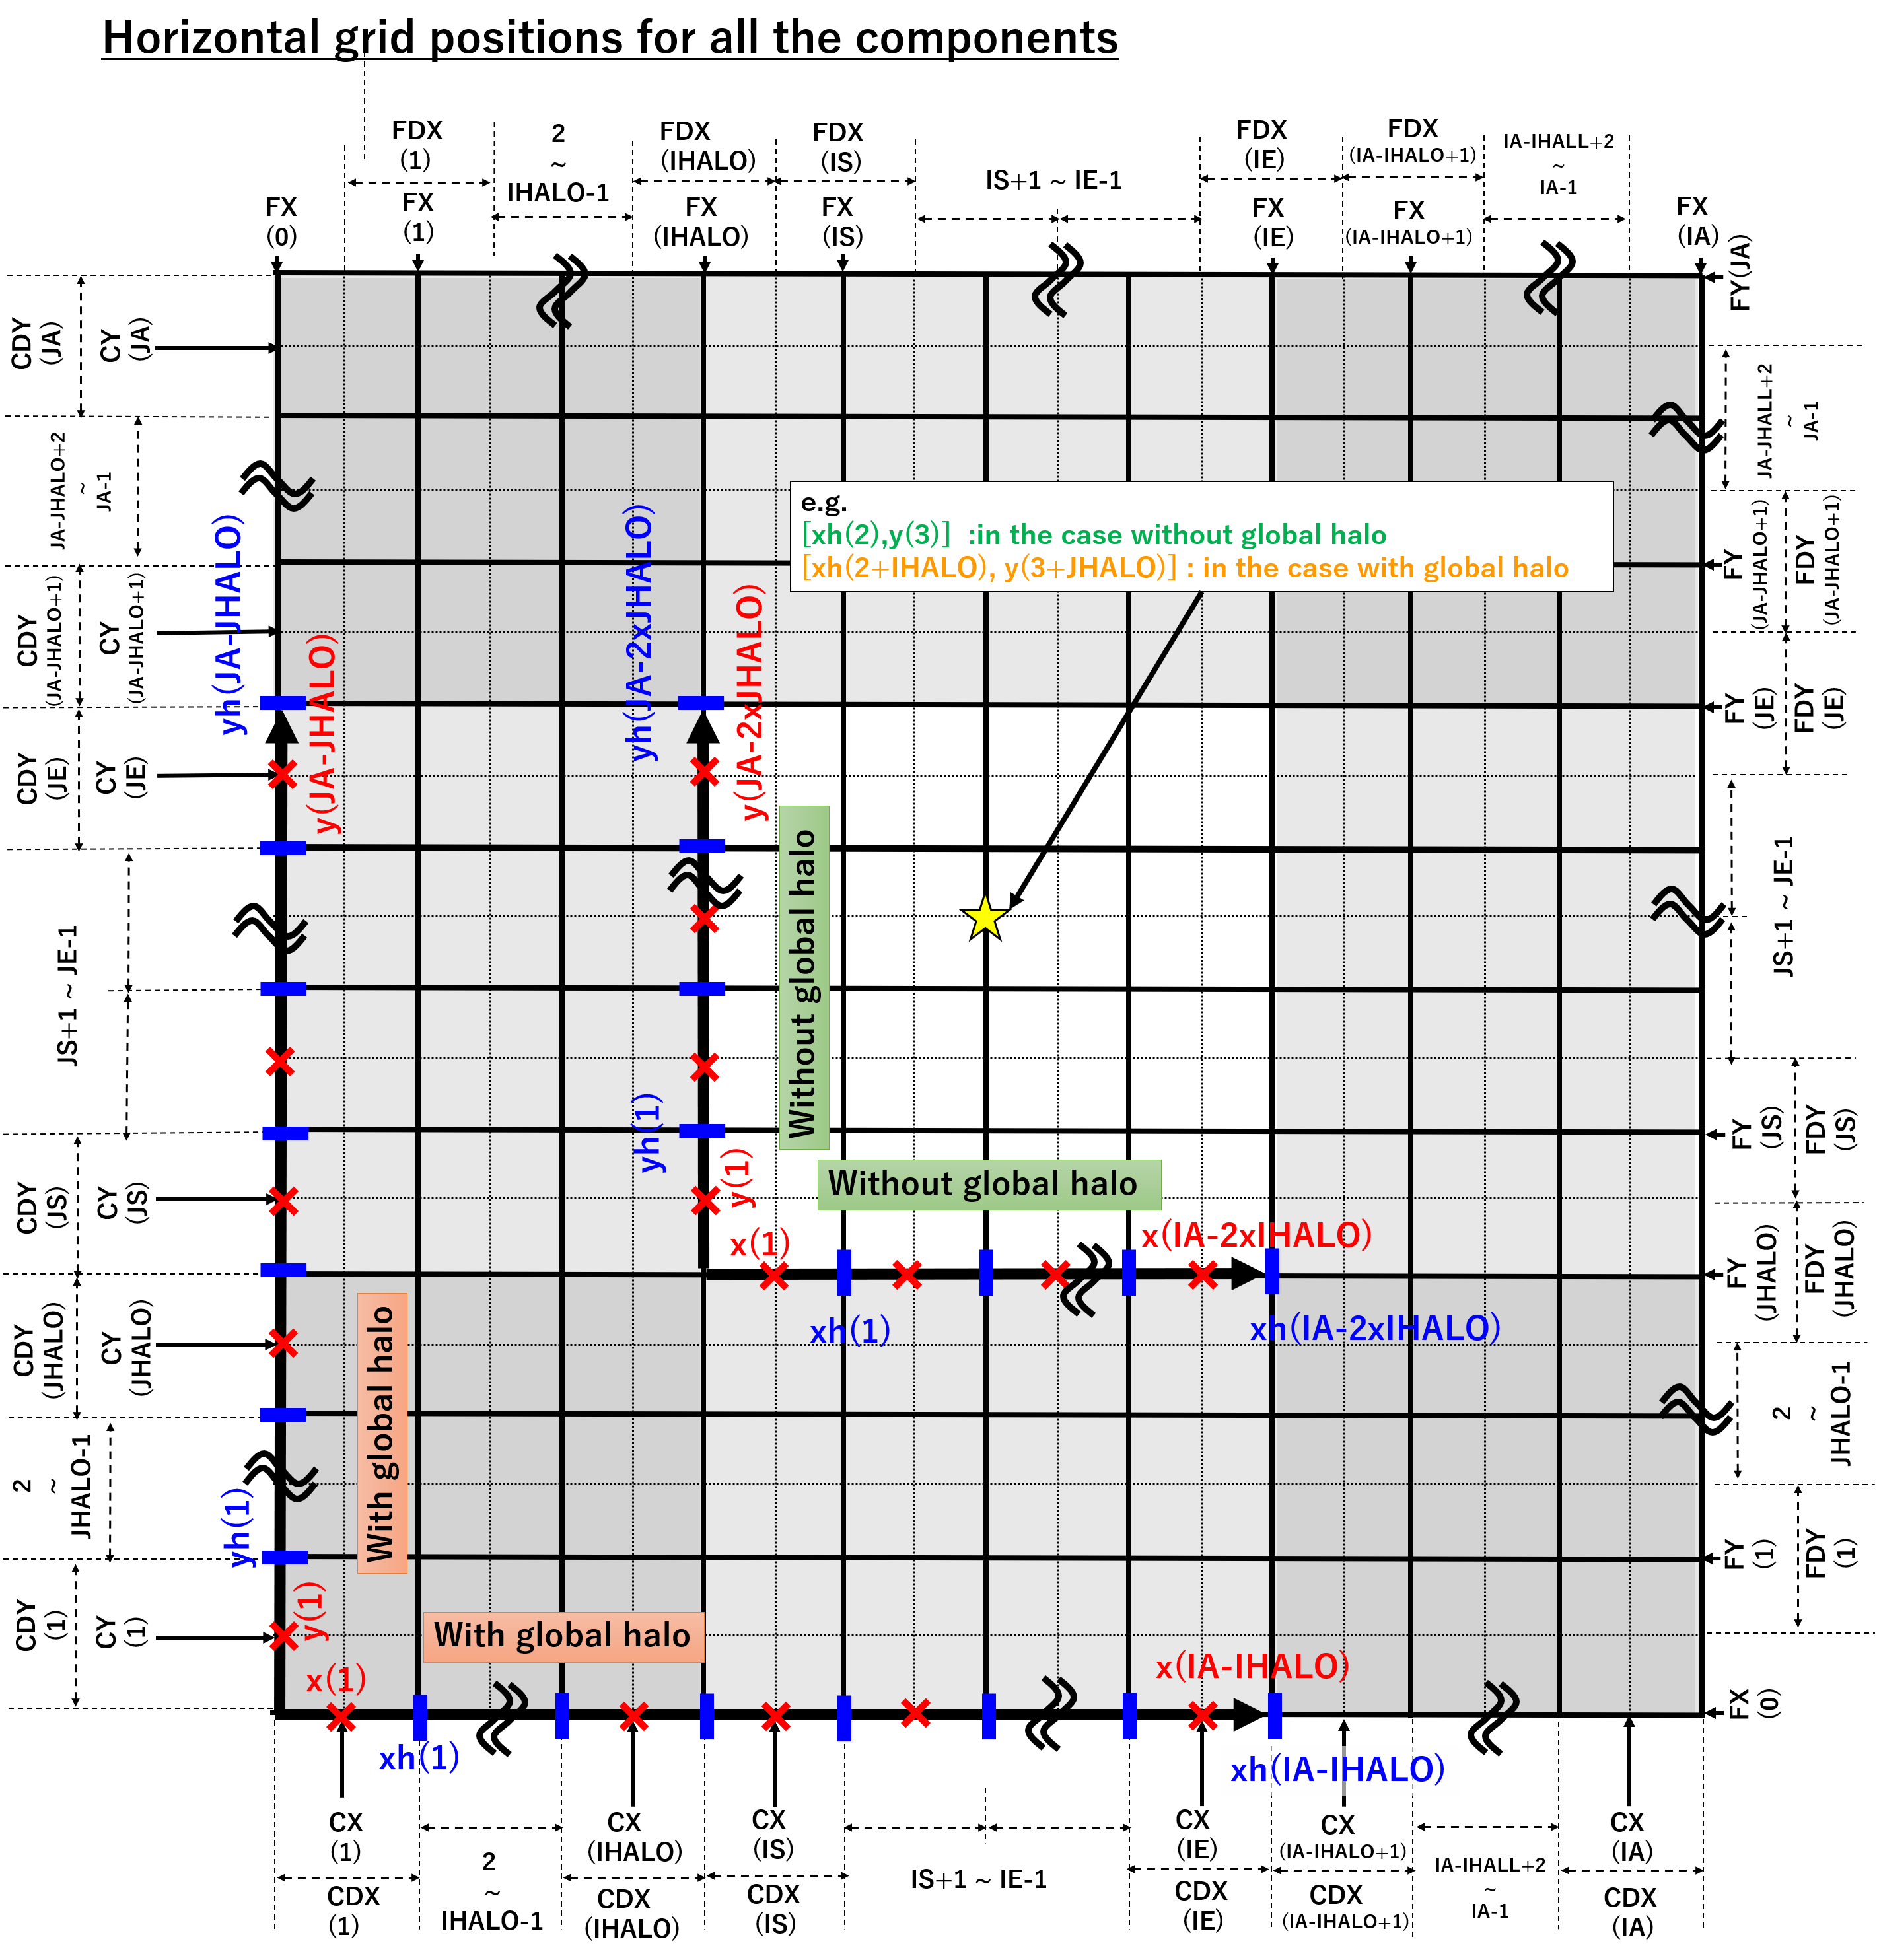
\includegraphics[width=1.0\hsize]{./figure/horizontal-coordinate-final2.png}\\
  \caption{Horizontal coordinate in \scalenetcdf file}
  \label{fig:netcdfhorizontalcoordinate}
\end{center}
\end{figure}
\begin{figure}[tbh]
\begin{center}
  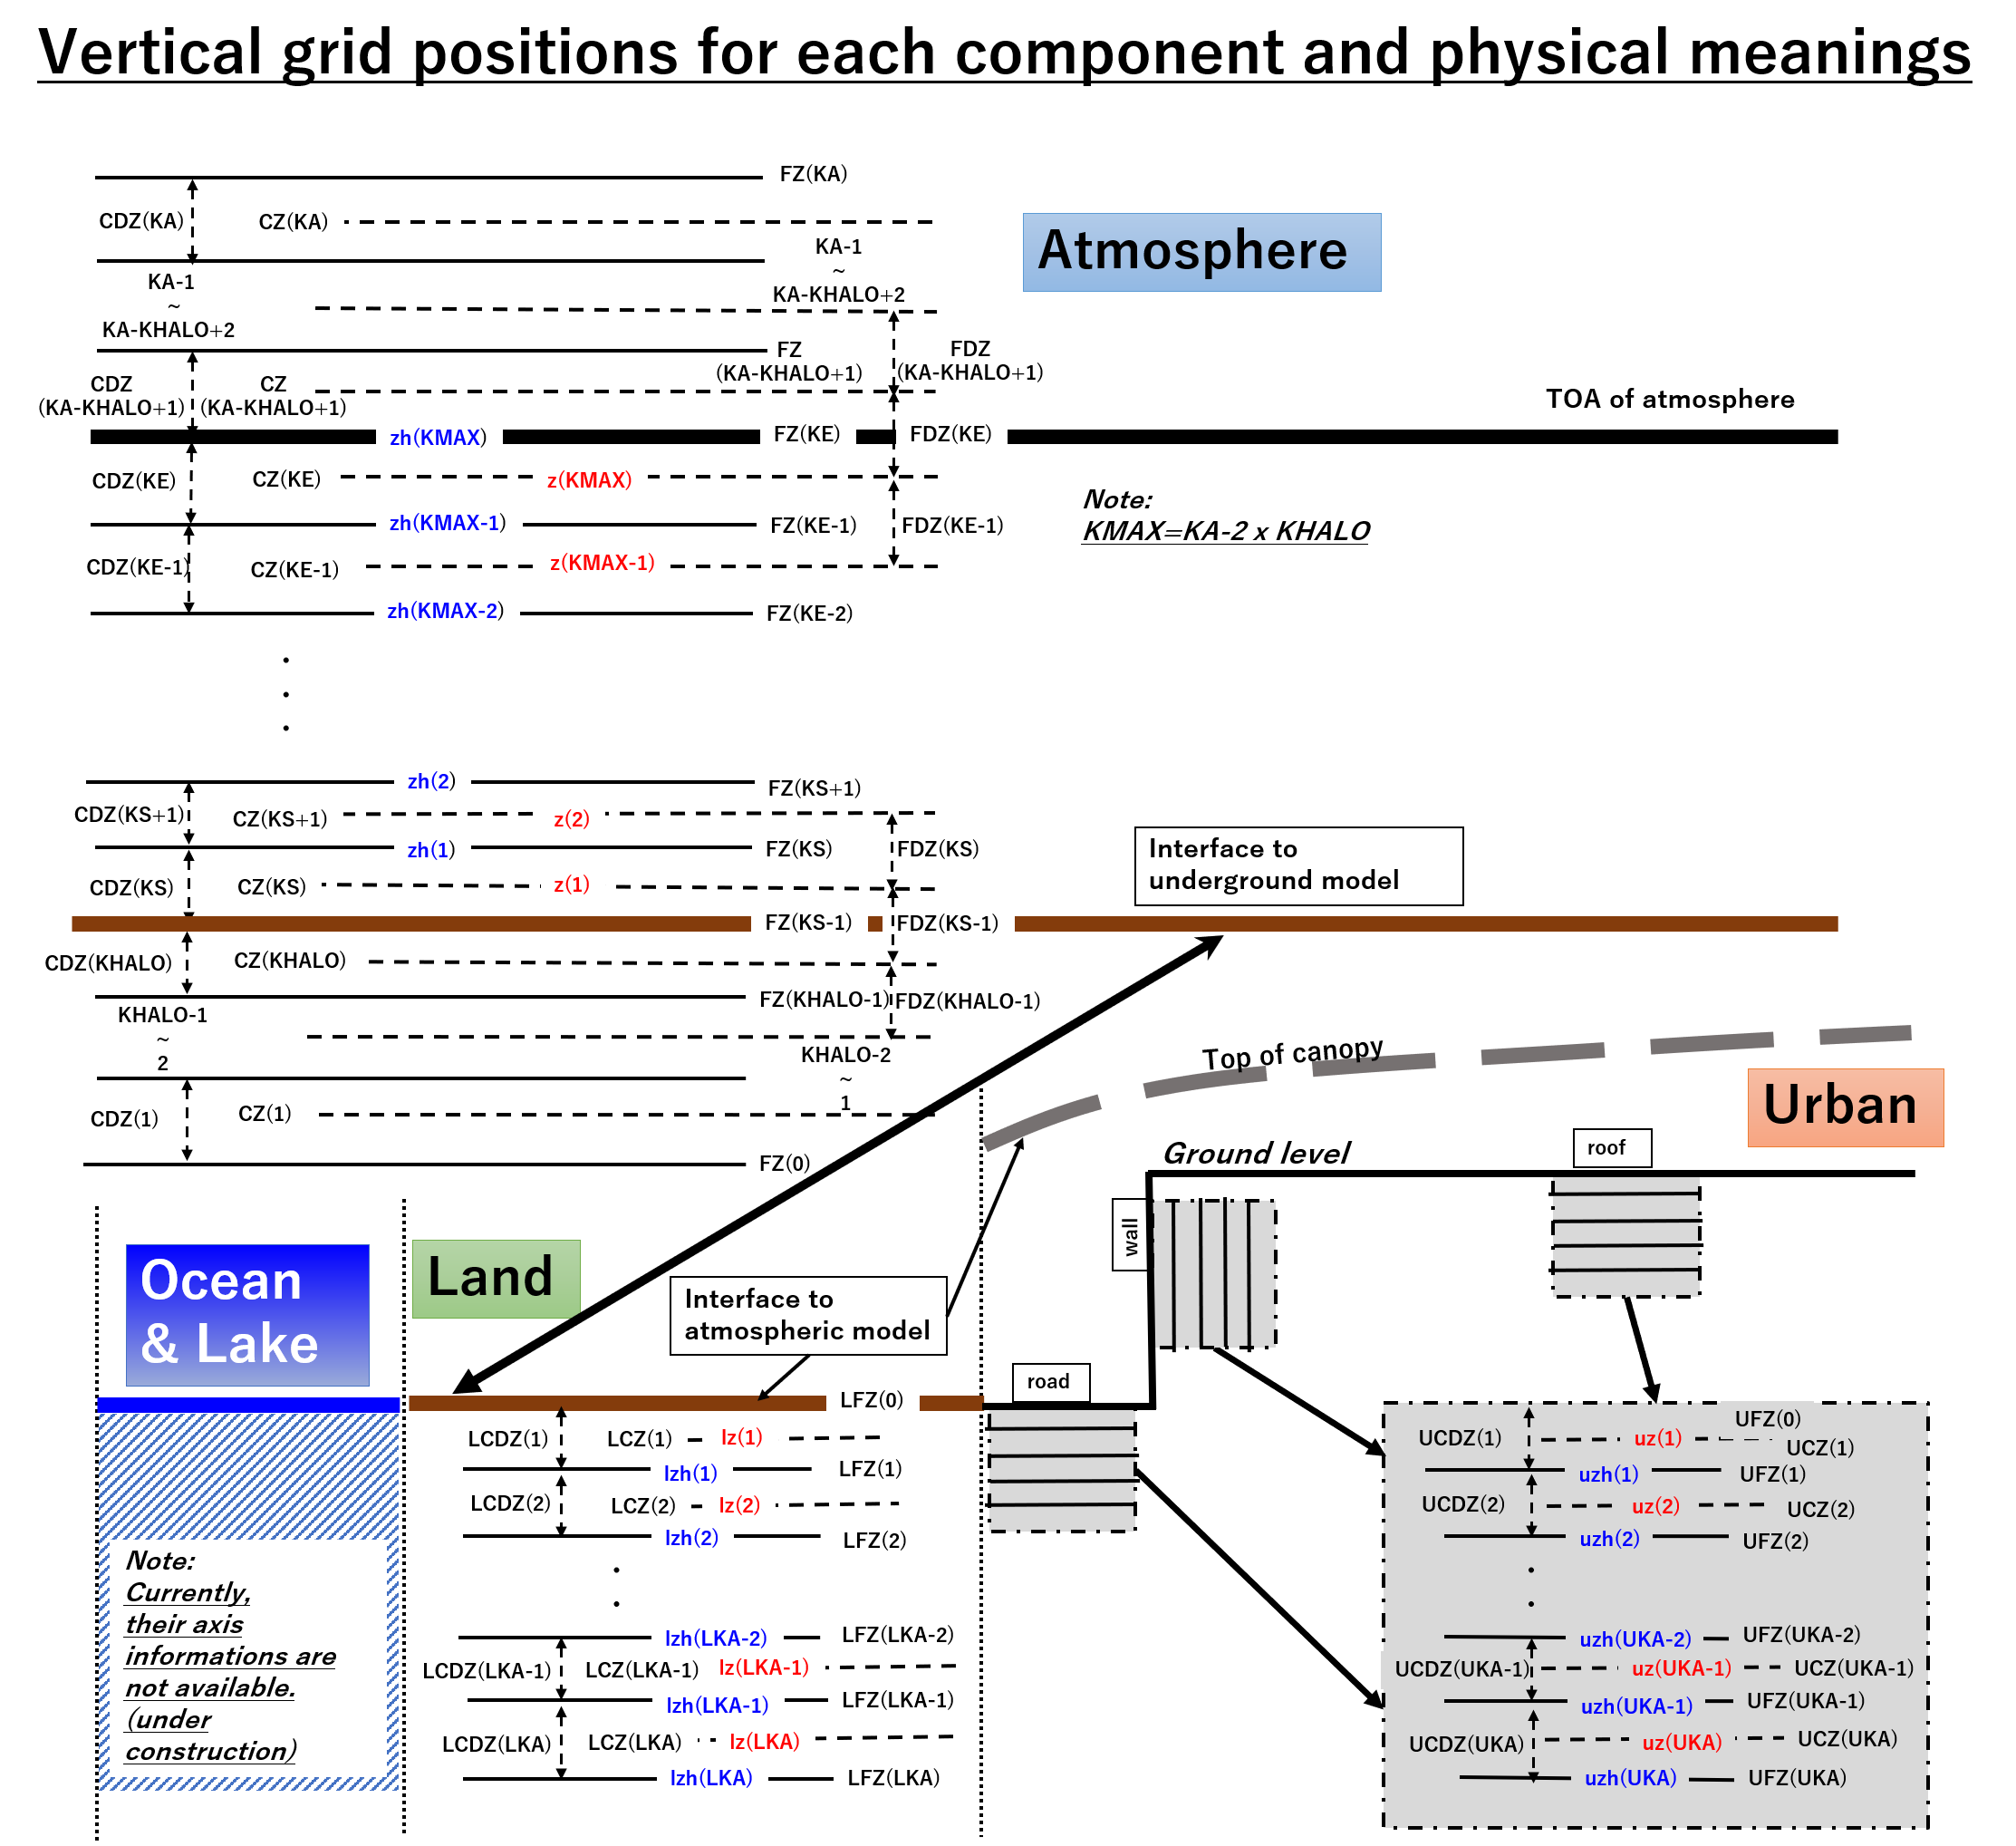
\includegraphics[width=1.0\hsize]{./figure/vertical_coordinate_final2.png}\\
  \caption{Horizontal coordinate in \scalenetcdf file}
  \label{fig:netcdfverticalcoordinate}
\end{center}
\end{figure}



\subsection{Data variables}
Data variables have attributes of the undefined value ``\_FillValue'' and 
the missing value ``missing\_value'' as well as ``long\_name'' and ``untis''.
Data structure in the initial (restart) data and boundary data files 
is identical to the array in the model, that is the z-x-y order.
On the other hand, it in the history data file is the x-y-z order.
This is true for 3D axis variables ( see also Table \ref{table:netcdf_axes} ).

 % 完了
 %In this chapter,
the data file convention used in \scalelib is explained.
\scalelib employs the data format devloped by Unidata
(\url{http://www.unidata.ucar.edu}) and utilizes \netcdf to
treat the SCALE native file.
\netcdf file format is self-descriptive and
can store any information required for data
with axis information in the file itself.
Since the data file does not have much less dependecy such as bit endian,
it is available on many machine that installs \netcdf. 
Unpon this format, there is some  convention peculiar to \scalelib.
The SCALE native file is referred to as SCALE-IO file.

\section{Global Attributes} 
In SCALE-IO file,
the explanation of data itself and spatial mesh information
are store as Global Attribute.

 %\input section{Binary data format for input data}
 %\input section{Data format for topography/landuse data}

 \chapter{ユーザーが作成したプログラムの組み込み方}
 \section{Module for user defined settings} \label{sec:mod_user}

\scalerm prepares many options, which users can specify as namelist parameters, to meet users' demand for their calculations.
However, when there is no option you desire,
you can modify model variables directly as you want by programming using the module for users, namely \verb|mod_user|.
This section describes what is \verb|mod_user| module and how to use it.


\subsection{What is \texttt{mod\_user} module}

The default \verb|mod_user| module is provided in \texttt{scale-{\version}/scale/scale-rm/src/user/mod\_user.F90}.\\
Prepare your own \verb|mod_user.F90| and then compile it instead of the default one.

The module must contain the following subroutines:
\begin{alltt}
  subroutine USER_tracer_setup
  subroutine USER_setup
  subroutine USER_mkinit
  subroutine USER_update
  subroutine USER_calc_tendency
\end{alltt}

\noindent This is the sequence of execution of the scale-rm.
\begin{alltt}
Initial setup
  IO setup
  MPI setup
  Grid settings
  Setup of administrator for dynamics and physics schemes 
  Tracer setup
  \textcolor{blue}{USER tracer setup}
  Setup topography, land
  Setup of vars and drivers for dynamics and physics schemes 
  \textcolor{blue}{USER setup}
Main routine
  Time advance
  Ocean/Land/Urban/Atmos update
  \textcolor{blue}{User update}
  Output restart
  Calculation of tendency in Atmos/Ocean/Land/Urban
  \textcolor{blue}{Calculation of tendency}
  History output
\end{alltt}
The timings for calling individual subroutines of the \verb|mod_user| are indicated by blue color.
The \verb|USER_mkinit| is called in the init program \verb|scale-rm_init|.


Since the subroutines in \verb|mod_user| are basically called after handling each process,
you can replace any settings and variables as you need.
You can also add several tracers, such as passive tracers, in \verb|USER_tracer_setup|.
%When you change settings defined in setup process, use \verb|USER_setup|.
%\textcolor{blue}{User update}
There are several examples of \verb|mod_user.F90| in the test cases (\texttt{scale-{\version}/scale-rm/test/case}).


\subsection{Compile}

To compile \scalerm with your \verb|mod_user.F90|, you can use the Makefile in the test cases as follows.\\
\texttt{ \$ cd scale-\version/scale-rm/test/case}\\
\texttt{ \$ mkdir -p your\_dir/exp\_name}\\
\texttt{ \$ cd your\_dir/exp\_name}\\
\texttt{ \$ cp ../../advection/500m/Makefile .}\\
Copy your \verb|mod_user.F90| to this directory.\\
\texttt{ \$ make}
 % 完了
 \chapter{\scalelib の使い方}
 \section{{\scalelib}を使用するユーザープログラム}

\scalelib はサブルーチンの集合体である。
これらのサブルーチンは、任意のプログラムで利用できる。
ライブラリファイルは、\scalelib をコンパイルした後に\texttt{scale-{\version}/lib/}の下に「\verb|scalelib.a|」として作成される。

以下は、ユーザがプログラム中で{\scalelib}を使用するときのテンプレートである。
\editbox{
  \verb|program template|\\
  \verb|  use scalelib|\\
  \verb|  implicit none|\\
  \verb||\\
  \verb|  call SCALE_init|\\
  \verb||\\
  \verb|  ! user instractions|\\
  \verb||\\
  \verb|  call SCALE_finalize|\\
  \verb||\\
  \verb|  stop|\\
  \verb|end program template|\\
}

以下は、ファイルから読み込まれた大気の物理量から対流有効位置エネルギー(CAPE)を計算する擬プログラムである。
メイン部分の前に、必要なモジュールを引用(use)し、また必要な入力変数を用意しなければならない。
以下の例は、プログラムの一部分であることに注意されたい。
\editbox{
  \verb|                         |\\
  \verb|use scale_const, only: & | \\
  \verb|      Rdry => CONST_Rdry, Rvap => CONST_Rvap, CPdry => CONST_CPdry|\\
  \verb|use scale_atmos_hydrometeor, only:  &  |\\
  \verb|      CPvap => CP_VAPOR, CL => CP_WATER|\\
  \verb|use scale_file, only:  &  | \\
  \verb|     FILE_open, FILE_read, FILE_close|\\
  \verb|use scale_atmos_adiabat, only:  & | \\
  \verb|     ATMOS_ADIABAT_setup, ATMOS_ADIABAT_cape|\\
  \verb|                  :      |\\
  \verb| real(8) :: z(kmax,imax,jmax), zh(0:kmax,imax,jmax)|\\
  \verb| real(8) :: temp(kmax,imax,jmax), pres(kmax,imax,jmax), dens(kmax,imax,jmax)|\\
  \verb| real(8) :: qv(kmax,imax,jmax), qc(kmax,imax,jmax), qdry(kmax,imax,jmax)|\\
  \verb| real(8) :: rtot(kmax,imax,jmax), cptot(kmax,imax,jmax)|\\
  \verb| real(8) :: cape(imax,jmax), cin(imax,jmax)|\\
  \verb| real(8) :: lcl(imax,jmax), lfc(imax,jmax), lnb(imax,jmax)|\\
  \verb|                  :      |\\
  \verb| call FILE_open( basename, fid )                ! ファイルを開く|\\
  \verb| call FILE_read( fid, 'height', z(:,:,:) )      ! full-level での高度データを読み込む|\\
  \verb| call FILE_read( fid, 'height_xyw', zh(:,:,:) ) ! half-level での高度データを読み込む|\\
  \verb| call FILE_read( fid, 'T', temp(:,:,:) )        ! 温度データを読み込む|\\
  \verb|                  : ! PRES, DENS, QV, QC を読み込む|\\
  \verb| call FILE_close( fid )  |\\
  \verb|                         |\\
  \verb|! CAPE を計算するために必要ないくつかの変数を計算する|\\
  \verb| qdry(:,:,:)  = 1.0D0 - qv(:,:,:) - qc(:,:,:)                            ! 乾燥空気の質量比|\\
  \verb| rtot(:,:,:)  = qdry(:,:,:) * Rdry + qv(:,:,:) * Rvap                    ! 気体定数\|\\
  \verb| cptot(:,:,:) = qdry(:,:,:) * CPdry + qv(:,:,:) * CPvap + ql(:,:,:) * CL ! 熱容量|\\
  \verb|                         |\\
  \verb| call ATMOS_ADIABAT_setup|\\
  \verb| call ATMOS_ADIABAT_cape( kmax, 1, kmax, imax, 1, imax, jmax, 1, jmax,      & ! 配列サイズ|\\
  \hspace{12em}\verb|             k0,                                               & ! percel initial layer|\\
  \hspace{12em}\verb|             dens(:,:,:), temp(:,:,:), pres(:,:,:),            & ! input|\\
  \hspace{12em}\verb|             qv(:,:,:), qc(:,:,:), qdry(:,:,:),                & ! input|\\
  \hspace{12em}\verb|             rtot(:,:,:), cptot(:,:,:),                        & ! input|\\
  \hspace{12em}\verb|             z(:,:,:), zh(:,:,:),                              & ! input|\\
  \hspace{12em}\verb|             cape(:,:), cin(:,:), lcl(:,:), lfc(:,:), lnb(:,:) ) ! output|\\
  \verb| |\\
}

リファレンスマニュアル(第\ref{sec:reference_manual}節を参照)では、利用できるサブルーチンの一覧やそれらのサブルーチンの詳細を確認できる。
ディレクトリ\texttt{scale-\version/scalelib/test/analysis}に、\scalerm が出力したヒストリファイルを解析するサンプルプログラムを用意してあるので、必要に応じて参照されたい。


\subsection{コンパイル}

\scalelib を用いたプログラムをコンパイルする前に、\scalelib をコンパイルする必要がある。\\
\texttt{ \$ cd scale-\version/scalelib/src}\\
\texttt{ \$ make}

ユーザーが作成したプログラムをコンパイルするときに、\texttt{scale-\version/lib}に置かれている
\verb|libscale.a|をリンクする必要がある。
また、モジュールファイルのパスをコンパイラに伝えなければならない。
モジュールファイルのパスは\texttt{scale-\version/include}であり、
このパスを指定するオプションはコンパイラに依存する。
オプションは、sysdep ディレクトリ下のファイル内で指定される変数 \verb|MODDIROPT| の値を見れば分かる(第\ref{subsec:environment}節を参照)。\\
\verb| $ ${FC} your-program ${MODDIROPT} scale-top-dir/include \\|\\
\verb|            `nc-config --cflags` -Lscale-top-dir/lib -lscale `nc-config --libs`|

ユーザーが作成したプログラムをコンパイルするために、サンプルにある Makefile を以下のように利用することもできる。\\
\texttt{ \$ cd scale-\version/scalelib/test/analysis}\\
\texttt{ \$ mkdir your\_dir}\\
\texttt{ \$ cd your\_dir}\\
\texttt{ \$ cp ../horizontal\_mean/Makefile .}\\
プログラムファイルを本ディレクトリにコピーする。\\
Makefile を編集する (BINNAME = your\_program\_name)。\\
\texttt{ \$ make}
 % 完了
 \section{リファレンスマニュアル} \label{sec:reference_manual}
\scalelib のサブルーチンに対するリファレンスマニュアルは、\url{https://scale.riken.jp/archives/\version/index.html}で公開している。
このリファレンスマニュアルは、doxgen (\url{http://www.doxygen.org/})によって生成されている.

リファレンスには、次の情報が含まれる。
\begin{itemize}
\item サブルーチン
\item ネームリストのパラメータ
\item ヒストリ(出力)変数
\end{itemize}


\subsection{サブルーチン}
サブルーチンの説明、引数、コールグラフがサブルーチンの情報として含まれる。
サブルチーンのソースコードも見ることができる。
ユーザーは、トップページやトップメニューにリンクされている「Module List」あるいは「File List」からサブルーチンを探し出すことができる。
モジュールのリストには、各モジュールに対する簡単な説明が書かれている。

モジュール名の接頭子は、\scalelib については「scale\_」、\scalerm については「mod\_」である。
ファイル名は、「.F90」の接尾子を付けたモジュール名である。
サブルーチン名は、接頭子を除いたモジュール名と関数を説明する名前からなる。
例えば、\verb|ATMOS_ADIABAT_cape|というサブルーチンは、ファイル\verb|scale_atmos_adiabat.F90|中のモジュール\verb|scale_atmos_adiabat|内に含まれる。

\editbox{
\verb|scale_atmos_adiabat.F90|\\
\\
\verb|module scale_atmos_adiabat| \\
\verb| ... ... | \\
\verb| contains| \\
\verb| !------------------------------------------|\\
\hspace{4em} \verb| subroutine atmos_adiabat_cape( & |\\
\hspace{8em} \verb| Kstr, &    | \\
\hspace{8em} \verb| DENS, &    | \\
\hspace{8em} \verb| ...        | \\
}


\subsection{ネームリストのパラメータ}
ネームリストのパラメータのリストは、リファレンスマニュアルのトップページにあるリンク先、
もしくは直接\url{https://scale.riken.jp/archives/\version/d5/d8a/namelist.html}に行くと見ることができる。
リストには、パラメータ名、ネームリストのグループ名、変数が定義されているモジュールの名前が含まれる。
パラメータは変数名で並び替えられている。
パラメータの詳細は、ネームリストのグループ名またはモジュール名をクリックすれば確認できる。

\begin{figure}[h]
\begin{center}
  \includegraphics[width=1.0\hsize]{./../../figure/doxygen_namelist.png}\\
  \caption{ネームリストのパラメータリストのWebページの例}
  \label{fig:doxygen_namelist}
\end{center}
\end{figure}

\newpage
\subsection{ヒストリ(出力)変数}
ヒストリ(出力)変数のリストは、リファレンスマニュアルのトップページにあるリンク先、または
直接\url{https://scale.riken.jp/archives/\version/dc/dd1/history.html}に行くと見ることができる。
リストには、変数名、簡単な説明、ヒストリデータのために変数が登録されているモジュールの名前が含まれる。
ヒストリ変数はモジュール名で並び替えられている。
変数の詳細情報は、モジュール名をクリックすれば確認できる。

\begin{figure}[h]
\begin{center}
  \includegraphics[width=1.0\hsize]{./../../figure/doxygen_history.png}\\
  \caption{ヒストリ(出力)変数リストのWebページの例}
  \label{fig:doxygen_history}
\end{center}
\end{figure}
 % 完了

 \chapter{バルクジョブの実行方法}
  %\section{How to Conduct Bulk Job}
%====================================================================================

\section{What's Bulk Job} \label{sec:bulkjob}
 \scalerm has a functionality for bulk jobs that allows simultaneous multiple execution of independent runs.
This function is useful for the parameter-sweep experiment, the ensemble experiment in different initial conditions, the time-slice climate simulation, and so on.

The bulk job function can be used not only for model simulation (\verb|scale-rm|), but also for the generation of topographical data, land-use data, and initial/boundary data. Note that the generation of topographical/land-use data by this function is limited to the case without a topography copy function (See \ref{subsec:nest_topo}).

In the following explanation, an independent execution in the bulk job is called a ``sub-job''.
Three two-domain nesting experiments are taken up as an example.
This set of experiments consists of three sub-jobs with different integration periods and calculation domain.
\nmitem{NUM_DOMAIN, PRC_DOMAINS, CONF_FILES} in \namelist{PARAM_LAUNCHER} in the file \verb|launch.conf| (refer to Section \ref{subsubsec:launch} ) must be the same in all configurations.
The other settings, such as integration time, the scheme used, and the number of grids per MPI process, do not need to be the same among the sub-jobs.

\begin{figure}[t]
\begin{center}
  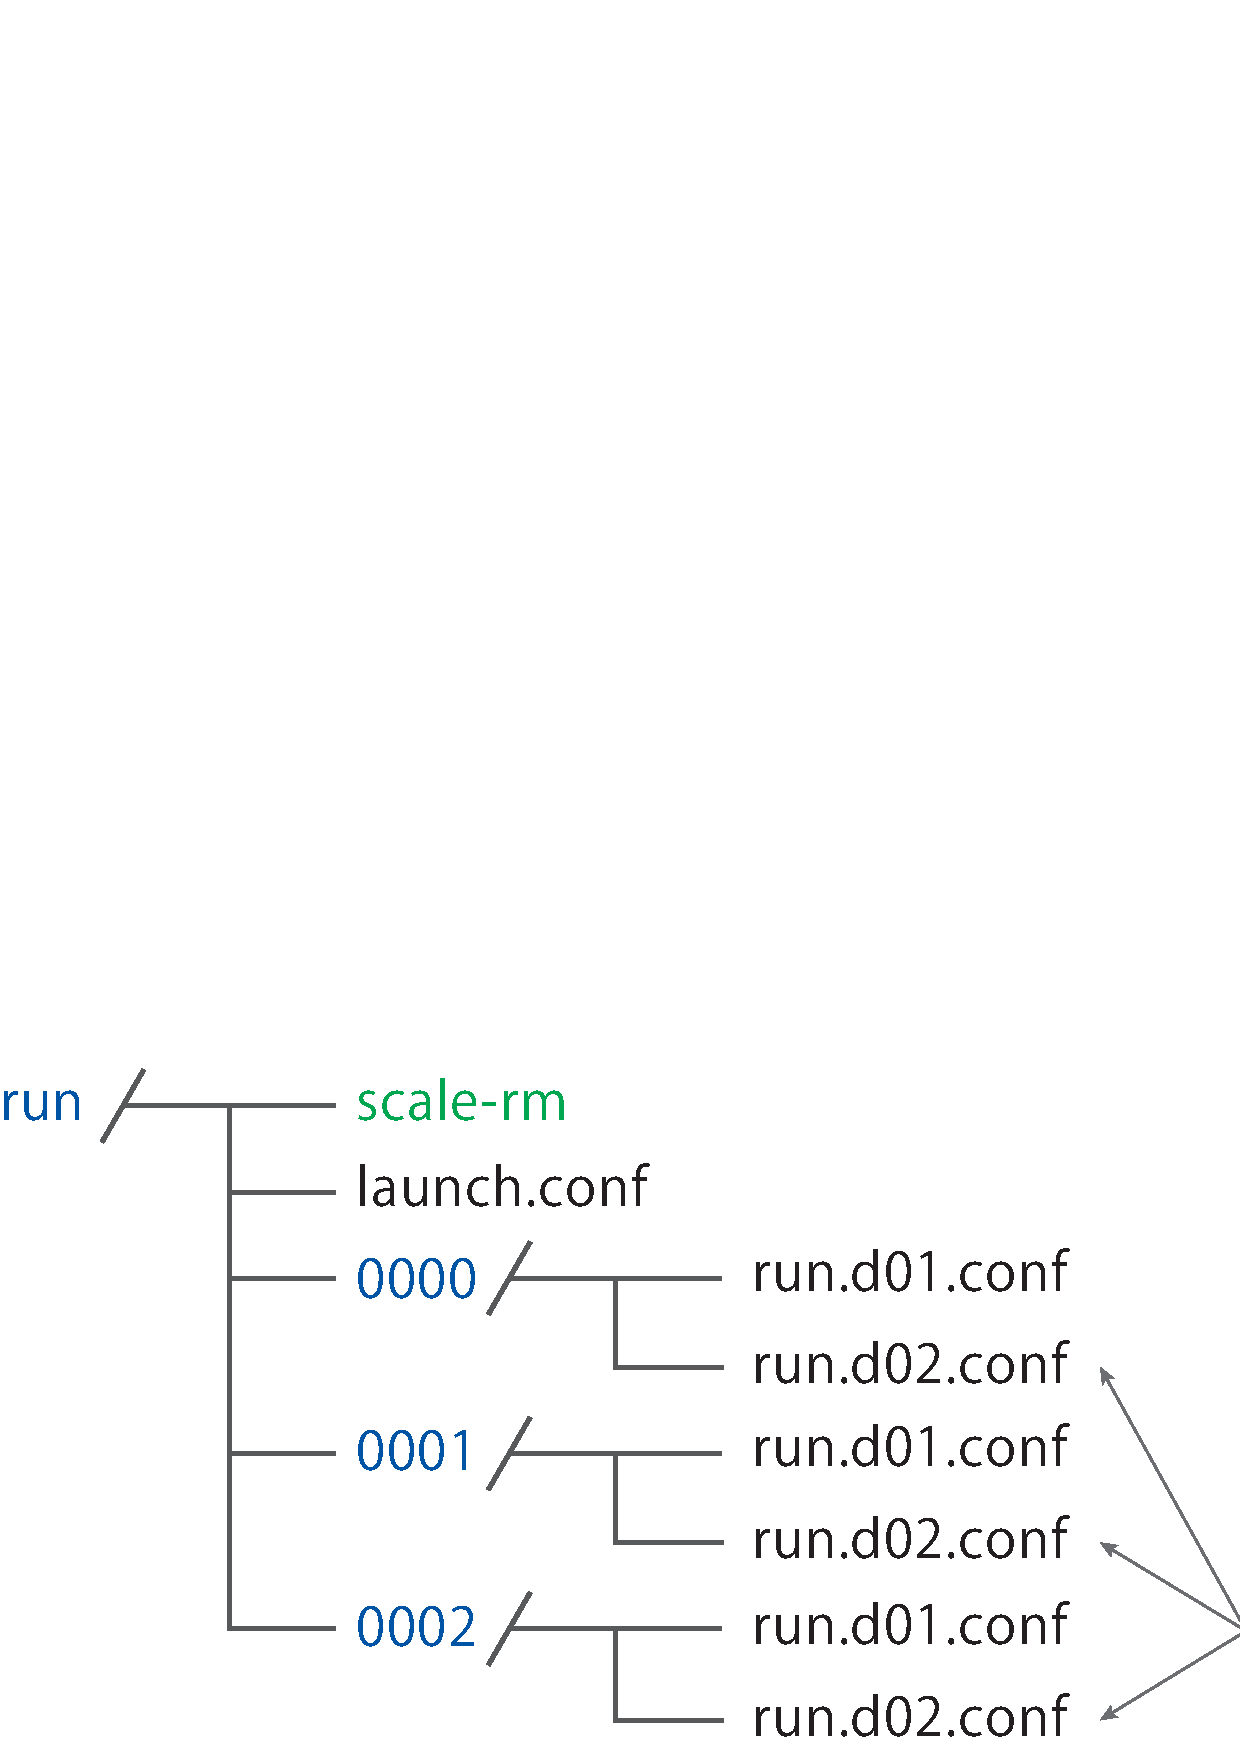
\includegraphics[width=0.6\hsize]{./../../figure/bulkjob_directory_structure.pdf}\\
  \caption{Structure of directories at the execution of \scalerm with bulk job.
Numbers such as ``0000'' are the directory names and called the job directory.   All necessary configuration files to execute sub jobs must be prepared in each job directory.
}
  \label{fig_bulkjob}
\end{center}
\end{figure}



\section{Settings for Bulk Job}
Since the bulk job function is an extension of the division and redistribution of MPI processes used in online nesting, file \verb|launch.conf| is required to launch the job. Even in case online nesting and bulk job functions are used together, only one file \verb|launch.conf| is required.
Below is an example of such a case.
\editboxtwo{
\verb|&PARAM_LAUNCHER|       & \\
\verb| NUM_BULKJOB = 3,|     & number of sub-jobs\\
\verb| NUM_ITERATION_BULK = 1,| & number of iterations to execute sub-jobs\\
\verb| BULKJOB_START_DIRNUM = 0,| & start number of the job directory\\
\verb| ADD_BULKJOB_PATH = .false.,| & add job directory to file names\\
\verb| NUM_DOMAIN  = 2,|     & number of nesting domains\\
\verb| PRC_DOMAINS = 9, 36,|  & number of total process in each domain\\
\verb| CONF_FILES  = run.d01.conf, run.d02.conf,| & name of configulation files\\
\verb| LOG_SPLIT   = .false.,| & log-output for mpi splitting?\\
\verb| COLOR_REORDER = .true.,| & coloring reorder for mpi splitting?\\
\verb| FAILURE_PRC_MANAGE = .false.,| & use failure process management?\\
\verb| NUM_FAIL_TOLERANCE = 1, | & tolerance number of failure processes\\
\verb| FREQ_FAIL_CHECK    = 5, | & FPM polling frequency per DT\\
\verb|/| \\
}
The number of sub-jobs is specified by \nmitem{NUM_BULKJOB}.
For single-domain experiments (no nesting), specify \nmitem{NUM_DOMAIN} $=$ 1.

The job directory name is a four-degit number, which by default corresponds to a job ID starting with 0.
You can change the starting number by specifing \nmitem{BULKJOB_START_DIRNUM}.

By default, the file names in the sub-job configuration files, such as \verb|init.conf| and \verb|run.conf|, must contain the job directory (e.g., \verb|0000/history.nc|).
If \nmitem{ADD_BULJJOB_PATH} is specified as \verb|.true.|, the job directory name will be added to all file names in the configuration files except the absolute path.

If your computer does not have enough resources to run all the sub-jobs at once, you can divide the sub-jobs into multiple groups.
The number of sub-jobs to be executed at one time will be \nmitem{NUM_BULKJOB} / \nmitem{NUM_ITERATION_BULK}.


The other configurations are described in Section \ref{subsubsec:launch}.


\section{Failure Process Management}
In the \scalerm bulk job system, a failure process management (FPM) tool is available. FPM watches the job groups with a polling interval.
If some jobs are unfortunately aborted, all other jobs are not aborted until the number of failure jobs reaches to the limit number.
\nmitem{FAILURE_PRC_MANAGE} is a switch for use FPM tool.
\nmitem{NUM_FAIL_TOLERANCE} and \nmitem{FREQ_FAIL_CHECK} are setting parameters for limit number of failure jobs and interval of checking failure job, respectively.
Note, this version of FPM tool is available only for single domain calculation, not available of full system for online-nesting calculation. If you want to use FPM tool even in online-nesting calculation,
\nmitem{NUM_FAIL_TOLERANCE} must be equal to the number of all jobs.


\section{Preparation for Bulk Job}
Prior to the execution of bulk jobs, prepare as many directories as the number of sub-jobs, which are called ``sub-directories.'' As in Fig. \ref{fig_bulkjob}, these correspond to \verb|0000/  0001/  0002/|. The directory name is assigned as a four-digit number starting from zero. In each directory, all the necessary files (configuration files, input files, and output directories) must be prepared.
Note that the path to directories or files specified in the configuration files must be correctly set up as explained below.
An excerpt of \verb|run.d01.conf| for job \verb|0000| are as follows:
\editbox{
\verb|&PARAM_IO| \\
\verb| IO_LOG_BASENAME = "0000/LOG_d01",| \\
\verb|/| \\
 \\
\verb|&PARAM_RESTART| \\
\verb| RESTART_OUTPUT       = .true.,| \\
\verb| RESTART_OUT_BASENAME = "0000/restart_d01",| \\
\verb| RESTART_IN_BASENAME  = "../init/0000/init_d01_00013046400.000",| \\
\verb|/| \\
 \\
\verb|&PARAM_GRAPHY| \\
\verb| TOPOGRAPHY_IN_BASENAME = "../pp/0000/topo_d01",| \\
\verb|/| \\
 \\
\verb|&PARAM_LANDUSE| \\
\verb| LANDUSE_IN_BASENAME = "../pp/0000/landuse_d01",| \\
\verb|/| \\
 \\
\verb|&PARAM_ATMOS_BOUNDARY| \\
\verb| ~ ... ~             | \\
\verb| ATMOS_BOUNDARY_IN_BASENAME    = "../init/0000/boundary_d01",| \\
\verb| ~ ... ~             | \\
\verb|/                    | \\
 \\
\verb|&PARAM_FILE_HISTORY| \\
\verb| FILE_HISTORY_DEFAULT_BASENAME  = "0000/history_d01",| \\
\verb| ~ ... ~           | \\
\verb|/| \\
}

As shown in Fig. \ref{fig_bulkjob}, job directories exist in the same hierarchy as the directory of the executable binary. That is, a configuration file exists under each job directory, whereas the input files and the output directories must be described as relative paths from the location of  the executable binary. The output directory in the 0000 experiment is \verb|0000/| and the name of output files are as \verb|0000/***|. {\color{blue}{ Note that when the file name is common to all experiments without adding the name of job directory, the output is written to the same file, and the data disappear as a result.
}}


%% バルクジョブの実行は, 全サブジョブを実行するのに必要なMPIプロセス数を指定し,
%% \begin{verbatim}
%%  $ mpirun  -n  135  ./scale-rm  launch.conf
%% \end{verbatim}
%% と行う。例では, 一つのサブジョブあたり, $9 + 36 = 45$プロセス使用し, 全体で3つのジョブを実行するので,
%% 総計で135プロセスを必要とする。
%% %
%% 実行すると得られるLOGファイルに, MPIプロセスを分割した時の情報が示されている。
%% LOGファイルを開くと, 最初の「SCALEロゴ」のあとに下記のようなメッセージが出力される。
%% 下記, ドメイン1のプロセス0からの出力例である。\\


\section{Execution of Bulk Job}

At the execution of bulk jobs, the total number of MPI processes is specified as

\begin{verbatim}
 $ mpirun  -n  135  ./scale-rm  launch.conf
\end{verbatim}
In this example, the number of processes per sub-job is 45 ($=9 + 36$) and the total number of processes used for three sub-jobs is 135. The message providing information regarding the division of MPI processes is written to the LOG files after the \scalelib logo. The following example is the log output for process 0 of Domain 1:
\msgboxtwo{
\verb| +++++ start making Cartesian topology|  & \\
\verb| *** UNIVERSAL_COMM_WORLD        :        0| &; different by execution environment\\
\verb| *** total process [UNIVERSAL]   :      135| &\\
\verb| *** my process ID [UNIVERSAL]   :       36| &\\
\verb| *** master rank?  [UNIVERSAL]   :        F| &\\
\verb| *** GLOBAL_COMM_WORLD           :        3| &; different by execution environment \\
\verb| *** total process [GLOBAL]      :       45| &\\
\verb| *** my process ID [GLOBAL]      :       36| &\\
\verb| *** master rank?  [GLOBAL]      :        F| &\\
\verb| *** LOCAL_COMM_WORLD            :        4| &; different by execution environment\\
\verb| *** total process [LOCAL]       :        9| &\\
\verb| *** my process ID [LOCAL]       :        0| &\\
\verb| *** master rank?  [LOCAL]       :        T| &\\
\verb| *** ABORT_COMM_WORLD            :        0| &\\
\verb| *** master rank ID [each world] :        0| &\\
&\\
}
The items belonging to \verb|[LOCAL]|, \verb|[GLOBAL]|, and \verb|[UNIVERSAL]| are the descriptions, respectively, of the process group in the domain, the nesting group, and the job group. The \verb|UNIVERSAL| group includes the \verb|GLOBAL| group and the \verb|GLOBAL| group includes the \verb|LOCAL| group. \verb|total process| represents the total number  of processes in each group and \verb|my process ID| is the ID of the process in the group.

It can be confirmed in this case that 1) since \verb|total process [UNIVERSAL]| is 135, all these processes are completed executed; 2) since \verb|total process [GLOBAL]| is 45, these 45 processes are used in a sub-job; 3) since the log file for Domain 1 is shown in this example, it is correct to describe \verb|total process [LOCAL]| as 9. If you see the log message for Domain 2,  it is 39. \verb|my process ID [UNIVERSAL]| is the process number  corresponding to the LOG and history files. Since this notation is the same as in the abnormal completion of execution, you can immediately recognize the processes in which errors occur during executing a considerable number of sub-jobs.


%%%%%%%%%%%%%%%%%%%%%%%%%%%%%%%%%%%%%%%%%%%%%%%%%%%%%%%%%%%%%%%%%%%%%%%%%%%%%%%%%%%%%%
 % 完了

\bibliographystyle{plainnat}
\bibliography{reference}

\begin{appendix}
%\chapter{ライブラリ環境のインストール} \label{achap:env_setting}
%%%%%%%%%%%%%%%%%%%%%%%%%%%%%%%%%%%%%%%%%%%%%%%%%%%%%%%%%%%%%%%%%%%%%%%%%%%%%%%%%%%%%%%%%%%%%

SCALEのインストールに必要なコンパイラやライブラリ環境のインストール方法について説明する。
ここでの記載内容は、こちらのテスト環境でのインストールプロセスを示しているものであって
必ずしも全く同じとは限らない。
うまくいかない場合には、それぞれのツール・ライブラリの開発元に直接問い合わせること。


Linuxをインストール後、各種プログラムのインストールはコマンドライン端末にて行う。
本書で説明するライブラリ環境のインストールでは、root権限が必要になる。
したがって、想定する環境は、ユーザーがroot権限を所持しているかサーバやデスクトップマシンである。
別途サーバー管理者が存在し、root権限を取得できない場合等は、必要な環境条件が整っているか
サーバー管理者に問い合わせること。

本節では、HDF5, NetCDF, MPIについてGNU compilerでコンパイルされたライブラリの説明を行う。
GNU compiler以外のIntel compilerなどを利用する場合は、各自でインストール方法を調べてインストールすること。\\

\noindent ここでインストールするコンパイラおよびライブラリ環境は、主に下記の4点である。
\begin{itemize}
\item GNU C/C++, fortran compiler
\item HDF5 Library (\url{https://www.hdfgroup.org/HDF5/})
\item NetCDF Library (\url{http://www.unidata.ucar.edu/software/netcdf/})
\item Message Passing Interface (MPI) Library (openMPI版、\url{http://www.open-mpi.org/})
\end{itemize}
これらのインストール方法について、本書では下記の5種類のOperating System (OS)について説明する。
\begin{itemize}
\item Linux CentOS 6.6 x86-64
\item Linux CentOS 7.1 x86-64
\item Linux openSUSE 13.2 x86-64
\item Apple Mac OS X 10.10 Yosemite
\item スーパーコンピュータ「京」
\end{itemize}
他のOSディストリビューション(下記参照)でもSCALEを利用可能だが、
本書でサポートするのは上記の範囲とする。\\

\noindent{\bf 動作確認済みの他のOSディストリビューション}
\begin{itemize}
\item Linux SUSE Enterprise Linux 11.1, 11.3 x86-64
\item Linux Vine Linux 6.3 x86-64
\item Linux Fedora 16 x86-64
\end{itemize}


\section{インストール方法 (Linux - CentOS 6.6-6.8 編)} \label{chap:install_centos}
%==========================================================================================

以下の説明で使用した環境は次のとおりである。
\begin{itemize}
\item CPU: Intel Core i5 2410M (sandybridge)
\item Memory: DDR3-1333 4GB
\item OS: CentOS 6.6 (kernel: 2.6.32-504.23.4.el6.x86\_64)\\
{\small *インストール時、"日本語"、 "Desktop"、"Kdump有り"を選択}
\end{itemize}

\subsubsection{ライブラリのインストール}

CentOS 6.6では、一部のライブラリをエンタープライズLinux用の拡張パッケージ(EPEL)リポジトリからインストールする。
そこで、はじめにEPELリポジトリをシステムにインストールし登録する。
CentOS 6.6では、ソフトウェアのインストールに"yum"コマンドを利用する。
すべての作業を行うまえに、下記のコマンドにてパッケージをアップデートしておくことをおすすめする。
\begin{verbatim}
 # yum update
\end{verbatim}

ルート権限で、下記のコマンドを実行することでリポジトリの登録が可能である。
\begin{verbatim}
 # yum install epel-release
\end{verbatim}
実行時のコマンドラインの様子は以下のようになる。
インストール対象がリストされるので、確認して"y"をタイプして先へ進める。\\

\noindent {\small {\gt
\fbox{
\begin{tabularx}{140mm}{l}
読み込んだプラグイン:fastestmirror, refresh-packagekit, security\\
インストール処理の設定をしています\\
Loading mirror speeds from cached hostfile\\
 * base: ftp.***.**.jp\\
 * extras: ftp.***.**.jp\\
 * updates: ftp.***.**.jp\\
依存性の解決をしています\\
-- トランザクションの確認を実行しています。\\
--- パッケージ epel-release.noarch 0:7-5 を インストール\\
-- 依存性解決を終了しました。\\
\\
依存性を解決しました\\
\\
======================================\\
 Package                アーキテクチャー バージョン      リポジトリー      容量\\
======================================\\
インストール中:\\
 epel-release           noarch           6-8             extras            14 k\\
\\
トランザクションの要約\\
======================================\\
インストール  1 パッケージ\\
\\
総ダウンロード容量: 14 k\\
インストール容量: 24 k\\
Is this ok (y/N): y\\
パッケージをダウンロードしています:
epel-release-6-8.noarch.rpm                                   14 kB     00:00\\
rpm\_check\_debug を実行しています\\
トランザクションのテストを実行しています\\
トランザクションのテストを成功しました\\
トランザクションを実行しています\\
  インストールしています  : epel-release-6-8.noarch                            1/1\\
  Verifying               : epel-release-6-8.noarch                            1/1\\
\\
インストール:\\
  epel-release.noarch 0:6-8\\
\\
完了しました!\\
\end{tabularx}
}}}\\

\noindent {\small *この時点で、yumによるインストールに失敗する場合は、
プロキシ設定等を含めた通信環境、yumリポジトリの登録状況等を再確認すること。}

\noindent yumのグループインストール機能を用いて,開発ツール
(ここでの対象は主にGNU compilerとmakeシステム)をまとめてインストールする。
\begin{verbatim}
 # yum groupinstall "development tools"
\end{verbatim}

\noindent つづいて、グループインストールではインストールされないライブラリを個別に追加する。
\begin{verbatim}
 # yum install zlib-devel
 # yum install hdf5-devel hdf5-static
 # yum install netcdf-devel netcdf-static
 # yum install openmpi-devel
 # yum install wgrib wgrib2
\end{verbatim}

SCALEは陰解法計算の部分で、数値計算ライブラリ Lapack
\footnote{\url{http://www.netlib.org/lapack/}}
を利用するオプションがある。
もし必要ならば、Lapack もインストールすること。
\begin{verbatim}
 # yum install lapack lapack-devel
\end{verbatim}

\noindent \textcolor{blue}{\small *wgrib、wgrib2は、第\ref{chap:tutorial_real}章:Tutorial: Real case で
外部入力データのプレ処理を行うために使用する。}

\noindent {\small *"yum -y install package name" のように ``-y'' オプションをつけて実行することで、インストール前の再確認をスキップできる。}


\subsubsection{環境変数の設定}

ローカルシステムでMPI並列プログラムを実行するために、OpenMPIライブラリの環境変数設定を行う。
ユーザ権限に移動して.bashrcをエディタで開き,
\begin{verbatim}
 $ vi ~/.bashrc
\end{verbatim}
下記をファイルの最後に追加して,環境変数の設定を記述する。\\

\noindent {\gt
\ovalbox{
\begin{tabularx}{140mm}{l}
 \\
 \verb|// ---------------- Add to end of the file ----------------|\\
 \verb|# OpenMPI|\\
 \verb|export MPI="/usr/lib64/openmpi"|\\
 \verb|export PATH="$PATH:$MPI/bin"|\\
 \verb|export LD_LIBRARY_PATH="$LD_LIBRARY_PATH:$MPI/lib"|\\
 \\
\end{tabularx}
}}\\

編集が終わったら、環境設定を有効にする。
\begin{verbatim}
 $ . ~/.bashrc
\end{verbatim}


%\subsubsection{Installation of GPhys}
%CentOSの場合、yumリポジトリに地球電脳倶楽部のGFD-Dennouリポジトリを登録することで、
%簡単にGPhysをインストールできる。
%root権限で、GFD-Dennouリポジトリを次のような内容で登録する。
%
%\begin{verbatim}
% # vi /etc/yum.repos.d/GFD-Dennou.repo
%\end{verbatim}
%
%\begin{verbatim}
% // ---------------- Edit the file ----------------
% [gfd-dennou]
% name=GFD DENNOU Club RPMS for CentOS $releasever - $basearch
% baseurl=http://www.gfd-dennou.org/library/cc-env/rpm-dennou/CentOS/$releasever/$basearch/
% enabled=1
% gpgcheck=0
%\end{verbatim}
%編集が終わったら、yumでGPhysをインストールする。
%\begin{verbatim}
% # yum install gphys
%\end{verbatim}


\section{インストール方法 (Linux - CentOS 7.1-7.2 編)} \label{chap:install_centos71}
%==========================================================================================

以下の説明で使用した環境は次のとおりである。
\begin{itemize}
\item CPU: Intel Core i5 2410M (sandybridge)
\item Memory: DDR3-1333 4GB
\item OS: CentOS 7.1 (kernel: 3.10.0-229.7.2.el7.x86\_64)\\
{\small *インストール時、"日本語"、 "Gnome デスクトップ"、"Kdump有り"を選択}
\end{itemize}

\subsubsection{ライブラリのインストール}

CentOS 7.1では、一部のライブラリをエンタープライズLinux用の拡張パッケージ(EPEL)リポジトリからインストールする。
そこで、はじめにEPELリポジトリをシステムにインストールし登録する。
CentOS 7.1では、ソフトウェアのインストールに"yum"コマンドを利用する。
すべての作業を行うまえに、下記のコマンドにてパッケージをアップデートしておくことをおすすめする。
\begin{verbatim}
 # yum update
\end{verbatim}

ルート権限で、下記のコマンドを実行することでリポジトリの登録が可能である。
\begin{verbatim}
 # yum install epel-release
\end{verbatim}
実行時のコマンドラインの様子は以下のようになる。
インストール対象がリストされるので、確認して"y"をタイプして先へ進める。\\

\noindent {\small {\gt
\fbox{
\begin{tabularx}{140mm}{l}
読み込んだプラグイン:fastestmirror, langpacks\\
base                                                      3.6 kB     00:00\\
extras                                                    3.4 kB     00:00\\
updates                                                   3.4 kB     00:00\\
Loading mirror speeds from cached hostfile\\
 * base: ftp.***.**.jp\\
 * extras: ftp.***.**.jp\\
 * updates: ftp.***.**.jp\\
依存性の解決をしています\\
-- トランザクションの確認を実行しています。\\
--- パッケージ epel-release.noarch 0:7-5 を インストール\\
-- 依存性解決を終了しました。\\
\\
依存性を解決しました\\
\\
======================================\\
 Package                アーキテクチャー バージョン      リポジトリー      容量\\
======================================\\
インストール中:\\
 epel-release           noarch           7-5             extras            14 k\\
\\
トランザクションの要約\\
======================================\\
インストール  1 パッケージ\\
\\
総ダウンロード容量: 14 k\\
インストール容量: 24 k\\
Is this ok (y/d/N): y\\
Downloading packages:\\
extras/7/x86\_64/prestodelta                                 7.6 kB   00:00\\
epel-release-7-5.noarch.rpm                                  14 kB   00:00\\
Running transaction check\\
Running transaction test\\
Transaction test succeeded\\
Running transaction\\
  インストール中          : epel-release-7-5.noarch                         1/1\\
  検証中                  : epel-release-7-5.noarch                         1/1\\
\\
インストール:\\
  epel-release.noarch 0:7-5\\
\\
完了しました!\\
\end{tabularx}
}}}\\

\noindent {\small *この時点で、yumによるインストールに失敗する場合は、
プロキシ設定等を含めた通信環境、yumリポジトリの登録状況等を再確認すること。}

\noindent yumのグループインストール機能を用いて,開発ツール
(ここでの対象は主にGNU compilerとmakeシステム)をまとめてインストールする。
\begin{verbatim}
 # yum groupinstall "development tools"
\end{verbatim}

\noindent つづいて、グループインストールではインストールされないライブラリを個別に追加する。
\begin{verbatim}
 # yum install hdf5-devel hdf5-static
 # yum install netcdf-devel netcdf-static
 # yum install netcdf-fortran-devel
 # yum install openmpi-devel
 # yum install wgrib wgrib2
\end{verbatim}

SCALEは陰解法計算の部分で、数値計算ライブラリ Lapack
\footnote{\url{http://www.netlib.org/lapack/}}
を利用するオプションがある。
もし必要ならば、Lapack もインストールすること。
\begin{verbatim}
 # yum install lapack lapack-devel
\end{verbatim}

\noindent \textcolor{red}{\small *fortran用のモジュールファイルは別パッケージになっている。
"netcdf-fortran-devel"のインストールを忘れないこと。}

\noindent \textcolor{blue}{\small *wgrib、wgrib2は、第\ref{chap:tutorial_real}章:Tutorial: Real case で
外部入力データのプレ処理を行うために使用する。}

\noindent {\small *"yum -y install package name"として実行することで、インストール前の再確認をスキップできる。}

\subsubsection{環境変数の設定}

ローカルシステムでMPI並列プログラムを実行するために、OpenMPIライブラリの環境変数設定を行う。
ユーザ権限に移動して.bashrcをエディタで開き,
\begin{verbatim}
 $ vi ~/.bashrc
\end{verbatim}
下記をファイルの最後に追加して,環境変数の設定を記述する。\\

\noindent {\gt
\ovalbox{
\begin{tabularx}{140mm}{l}
 \\
 \verb|// ---------------- Add to end of the file ----------------|\\
 \verb|# OpenMPI|\\
 \verb|export MPI="/usr/lib64/openmpi"|\\
 \verb|export PATH="$PATH:$MPI/bin"|\\
 \verb|export LD_LIBRARY_PATH="$LD_LIBRARY_PATH:$MPI/lib"|\\
 \\
\end{tabularx}
}}\\

編集が終わったら、環境設定を有効にする。
\begin{verbatim}
 $ . ~/.bashrc
\end{verbatim}


\section{インストール方法 (Linux - openSUSE 13.2 編)} \label{chap:install_opensuse}
%==========================================================================================

以下の説明で使用した環境は次のとおりである。
\begin{itemize}
\item CPU: Intel Core i5 2410M (sandybridge)
\item Memory: DDR3-1333 4GB
\item OS: openSUSE 13.2 (kernel: 3.16.7-21-desktop x86\_64)\\
{\small *インストール時、"日本語"、 "Gnome Desktop"を選択}
\end{itemize}

\subsubsection{ライブラリのインストール}

openSUSE 13.2では、一部のライブラリを外部リポジトリ
(ocefpaf's Home Project; \url{https://build.opensuse.org/project/show/home:ocefpaf})からインストールする。
このため、まずhome\_ocefpafリポジトリをシステムにインストールし登録する。
このリポジトリには、grads、ncview、GMT、ncl、そしてcdoといったツール群も含まれており便利である。

openSUSE 13.2では、ソフトウェアのインストールに"zypper"コマンドを利用する。
openSUSEでは一般にユーザーがrootユーザーにスイッチすることを推奨しておらず、
デフォルトのままOSをインストールすると"su"コマンドによってrootユーザーに
スイッチすることはできないので、"sudo"コマンドを利用してインストール作業を行う。
すべての作業を行うまえに、下記のコマンドにてパッケージをアップデートしておくことをおすすめする。
\begin{verbatim}
 # sudo zypper update
\end{verbatim}

下記のコマンドを実行することでリポジトリの登録が可能である。
\begin{verbatim}
 $ sudo zypper ar \\
   http://download.opensuse.org/repositories/home:/ocefpaf/openSUSE_13.2/ \\
   home_ocefpaf
\end{verbatim}
{\small *上記コマンド中の"\verb|\\|"は、組版上の改行であることを意味する。
実際は改行も"\verb|\\|"の記述も必要ない。}
実行時のコマンドラインの様子は以下のようになる。\\

\noindent {\small {\gt
\fbox{
\begin{tabularx}{140mm}{l}
 リポジトリ 'home\_ocefpaf' を追加しています ...............................完了 \\
 リポジトリ 'home\_ocefpaf' を正常に追加しました\\
 有効         : はい (Y)\\
 自動更新     : いいえ (N)\\
 GPG チェック : はい (Y)\\
 URI          : \url{http://download.opensuse.org/repositories/home:/ocefpaf/openSUSE_13.2/}
\end{tabularx}
}}}\\

{\small *この時点で、zypperによるインストールに失敗する場合は、
プロキシ設定等を含めた通信環境、zypperリポジトリの登録状況等を再確認すること。}

\noindent zypperのパターンインストール機能を用いて,基本開発ツール
(ここでの対象は主にGNU compilerとmakeシステム)をまとめてインストールする。
\begin{verbatim}
 $ sudo zypper install --type pattern devel_basis
\end{verbatim}

home\_ocefpafリポジトリを登録して最初のインストールの場合、
下記のようにパッケージの署名鍵の信頼について問われることがある。
"a"の「ずっと信頼」を選択して作業を進める。
その後、インストール対象がリストされるので、確認して"y"をタイプして先へ進める。\\

\noindent {\small {\gt
\fbox{
\begin{tabularx}{140mm}{l}
 鍵を拒否しますか (R)? 一時的に信頼しますか (T)? \\
 それとも今後ずっと信頼しますか (A)? [r/t/a/? 全てのオプションを表示] (r): a
\end{tabularx}
}}}\\

\noindent つづいて、devel\_basisパッケージに含まれないライブラリを個別に追加する。
\begin{verbatim}
 $ sudo zypper install gcc-fortran
 $ sudo zypper install hdf5-devel hdf5-devel-static
 $ sudo zypper install netcdf-devel netcdf-devel-static
 $ sudo zypper install netcdf-fortran-devel netcdf-fortran-static
 $ sudo zypper install openmpi-devel openmpi-devel-static
 $ sudo zypper install wgrib wgrib2
\end{verbatim}

SCALEは陰解法計算の部分で、数値計算ライブラリ Lapack
\footnote{\url{http://www.netlib.org/lapack/}}
を利用するオプションがある。
もし必要ならば、Lapack もインストールすること。
\begin{verbatim}
 $ sudo zypper install lapack-devel lapack-devel-static
\end{verbatim}

\noindent \textcolor{blue}{\small *wgrib、wgrib2は、第\ref{chap:tutorial_real}章:Tutorial: Real case で
外部入力データのプレ処理を行うために使用する。}


\subsubsection{環境変数の設定}

ローカルシステムでMPI並列プログラムを実行するために、OpenMPIライブラリの環境変数設定を行う。
ユーザ権限に移動して.bashrcをエディタで開き,
\begin{verbatim}
 $ vi ~/.bashrc
\end{verbatim}
下記をファイルの最後に追加して,環境変数の設定を記述する。\\

\noindent {\gt
\ovalbox{
\begin{tabularx}{140mm}{l}
 \\
 \verb|// ---------------- Add to end of the file ----------------|\\
 \verb|# OpenMPI|\\
 \verb|export MPI="/usr/lib64/mpi/gcc/openmpi"|\\
 \verb|export PATH="$PATH:$MPI/bin"|\\
 \verb|export LD_LIBRARY_PATH="$LD_LIBRARY_PATH:$MPI/lib64"|\\
 \\
\end{tabularx}
}}\\

編集が終わったら、環境設定を有効にする。
\begin{verbatim}
 $ . ~/.bashrc
\end{verbatim}


\section{インストール方法(Mac OS X 編)} \label{chap:install_mac}
%==========================================================================================

\subsubsection{macportsを用いたインストール}

Apple Mac OS XでのSCALE実行環境を整備する方法について説明する。
ここではMac OS Xのパッケージマネージャの一つであるmacportsを用いる方法を紹介する。
その他の主要なパッケージマネージャとしては、homebrewが挙げられる。homebrewを利用しても環境は手軽に揃えられるので、
興味のある方は利用してもらいたい。

まずはAppleの開発ツールであるXcodeをインストールする。
大元のgccコンパイラを導入するために、必ずインストールする必要がある。
最近のOSのバージョンのものは、App Store経由で入手できる(無料)。
古いOSでは、インストールディスクから追加することが出来る。
最近のOSのXcodeの場合、最初に以下の様な設定をターミナルから行う必要がある。
\begin{verbatim}
 コマンドラインツールのインストール
 # xcode-select --install
\end{verbatim}
\begin{verbatim}
 ライセンス条項の承認(root権限必要)
 # sudo xcodebuild -license
\end{verbatim}

次にmacports本体をインストールする。
\url{https://www.macports.org/}
必要なパッケージインストーラーをダウンロードし、インストールを進める。\\
macportsとmacportsが管理するパッケージは/opt/local以下に配置される。
インストール時に\verb|.bash_profile|に、/opt/local/binへのパスが張られているので確認されたい。
macportsはコマンドラインから操作する。主要なコマンドは以下の通り。

\begin{verbatim}
 インストール可能なソフトウェアを検索する
 $ port search <検索文字>
\end{verbatim}
\begin{verbatim}
 ソフトウェアのインストール時に選択可能なオプション(variants)を確認する
 $ port variants <アプリ名>
\end{verbatim}
\begin{verbatim}
 ソフトウェアのインストール(root権限必要)
 $ sudo port install <アプリ名> [variants]
\end{verbatim}
\begin{verbatim}
 ソフトウェアのアンインストール(root権限必要)
 $ sudo port uninstall <アプリ名> [variants]
\end{verbatim}
\begin{verbatim}
 macports本体とパッケージカタログの更新(root権限必要)
 $ sudo port selfupdate
\end{verbatim}
\begin{verbatim}
 パッケージの更新(root権限必要)
 $ sudo port upgrade outdated
\end{verbatim}
\begin{verbatim}
 不要なパッケージ(activateされていない過去のバージョン等)の削除
 $ sudo port -u uninstall
\end{verbatim}

\subsubsection{gccからNetCDFまでのインストール}

macportsはパッケージの依存関係を解決してくれるが、必要なvariantsを備えたセットを作るには、
順番にインストールしていく方が問題が少ない。以下にsudo port installしていく順番とvariantsの設定を示す。
この例ではgcc4.9を利用する。
\begin{verbatim}
 $ gcc49
 $ openmpi-gcc49 +threads
 $ hdf4 +gcc49 +szip
 $ hdf5 +gcc49 +szip +fortran +cxx +openmpi +threadsafe
 $ netcdf +gcc49 +openmpi +netcdf4 +hdf4
 $ netcdf-fortran +gcc49 +openmpi
\end{verbatim}

macportsでは複数のコンパイラとMPIライブラリをインストール出来るため、
その中で利用するものを選択する必要がある。
今回の場合、gccとMPIライブラリが該当する。
この操作を行うと、gfortran等の一般的な名前でエイリアスが作られてPATHが通るようになる。
\begin{verbatim}
 $ sudo port select --set gcc mp-gcc49
 $ sudo port select --set mpi openmpi-gcc49-fortran
\end{verbatim}

インストールしたNetCDFライブラリを用いるときのPATHの設定は以下の通りである。
\verb|.bash_profile| をエディタで開き、
\begin{verbatim}
 $ emacs ~/.bash_profile
\end{verbatim}
下記をファイルに追加して、環境変数の設定を記述する。

\noindent {\gt
\ovalbox{
\begin{tabularx}{140mm}{l}
 \\
 \verb|export NETCDF_INCLUDE="-I/opt/local/include"|\\
 \verb|export NETCDF_LIBS="-L/opt/local/lib -lnetcdff -L/opt/local/lib -Wl,-headerpad_max_install_names -lnetcdf"|\\
 \\
\end{tabularx}
}}\\

SCALEは陰解法計算の部分で、数値計算ライブラリを利用するオプションがある。
もし必要ならば、macportsからATLASをインストールすることが出来る。
\begin{verbatim}
 $ atlas +gcc49
\end{verbatim}

追加する環境変数の設定は以下の通りである。

\noindent {\gt
\ovalbox{
\begin{tabularx}{140mm}{l}
 \\
 \verb|export LAPACK_LIBS="-L/opt/local/lib -llapack -lcblas -lf77blas -latlas"|\\
 \\
\end{tabularx}
}}\\

\subsubsection{Mac OS XにおけるGPhys / Ruby-DCLのインストール}

GphysはRubyのパッケージ管理システムRubyGemsを通してインストールできる。
詳細な情報については、(\url{https://www.hdfgroup.org/HDF5/})を参照されたい。
まず必要であればrubyのインストールをmacportsを用いて行う。この例ではRuby2.1を利用することにする。

\begin{verbatim}
 $ sudo port install ruby21
 $ sudo port select --set ruby ruby21
\end{verbatim}

次にmacportsを用いて、Gphysに必要なライブラリをインストールする。

\begin{verbatim}
 $ sudo port install fftw-3
 $ sudo port install gsl
 $ sudo port install C-DCL6
\end{verbatim}

最後にRubyGemsを用いて、Gphysをインストールする。

\begin{verbatim}
 $ sudo gem install gphys
\end{verbatim}

%\subsubsection{Mac OS XにおけるGrADSのインストール}(Todo)

\subsubsection{Mac OS Xでの実行時の注意点}

Mac OS Xを用いて\scalerm プログラムを実行すると、実行時に
「アプリケーション"scale-rm"へのネットワーク受信接続を許可しますか?」
というダイアログが出ることがあります。
これはコンパイルしたバイナリがマシンをまたいだMPI通信をするかファイアウォール機能が確認するためです。
コンパイルし直すたびにMPI並列数の分だけダイアログが出てきてしまいますが、今のところ表示を回避するためには
「システム環境設定」の「セキュリティとプライバシー」項目で「ファイアウォール」のタブを選択し、
プログラムの実行時にファイアウォールを切る方法しかありません。



\section{インストール方法 (スーパーコンピュータ「京」 編)} \label{chap:install_supercom}
%==========================================================================================

以下の説明で使用した環境は次のとおりである。
\begin{itemize}
\item 計算機: スーパーコンピュータ「京」
\item 言語環境: K-1.2.0-18
\end{itemize}

\subsubsection{ライブラリについて}
スーパーコンピュータ「京」では、SCALEのコンパイルに
必要なライブラリがAICSソフトウェアとして準備されている。
詳細は、京ポータルサイトの「AICSソフトウェア等」の項目、もしくは下記のWebページを参照のこと。\\
\noindent \url{http://www-sys-aics.riken.jp/releasedsoftware/ksoftware/pnetcdf.html}

一般に、スーパーコンピュータ「京」におけるSCALEのコンパイルには、\\
\noindent "\verb|/opt/aics/netcdf/k-serial-noszip/|"下にあるHDF5、NetCDFライブラリを用いる。
コンパイラやMPIライブラリについてもスーパーコンピュータ「京」専用のコンパイラとライブラリを用いるため、
特別にライブラリ環境を準備する必要はない。

\noindent {\small *コンパイル時に参照するライブラリのPATHは、
SCALEコンパイル時に使用する"Makedef.K"に記述されているため、
環境変数について特に設定する必要はない。}


\section{描画ツールのインストール} \label{chap:install_drawtool}
\label{sec:env_vis_tools}
%==========================================================================================

SCALEの計算結果や、初期値/境界値データなどを描画するのに利用可能である描画ツールの例を挙げる。
個人の好みでどのツールを使ってもよいし、出力形式を理解していれば、
ここに挙げた以外のツールで解析・描画することももちろん可能である。

\begin{itemize}
\item GPhys / Ruby-DCL by 地球電脳倶楽部\\
 \begin{itemize}
  \item URL: \url{http://ruby.gfd-dennou.org/products/gphys/}
  \item 概略:SCALEの出力ファイルは、MPI並列の計算領域分割に従ってMPIプロセスごとに
              NetCDF形式の分割ファイルとして出力される。GPhysの"gpview"や"gpvect"といった
              描画ツールを使えば、分割ファイルを後処理なしに直接開いて描画することができる。
  \item インストール方法:
  地球電脳倶楽部のWebページに、主なOSでのインストール方法についての解説がある。\\
  \url{https://www.gfd-dennou.org/library/ruby/tutorial/install/index-j.html}\\
  本書で使用したCentOS6、CentOS7については、下記のWebページにインストール方法が記載されている。\\
  \url{http://www.gfd-dennou.org/library/cc-env/rpm-dennou/index.html.ja}\\
   Mac OS Xにおけるインストール方法は第\ref{chap:install_mac}節で説明している他、
   \url{https://www.gfd-dennou.org/library/ruby/products/macports/index-j.html}
   でも解説されている。
   \end{itemize}
\item Grid Analysis and Display System (GrADS) by COLA\\
 \begin{itemize}
  \item URL: \url{http://iges.org/grads/}
  \item 概略:言わずと知れた描画ツール。SCALEのNetCDF形式の分割ファイルをそのまま読むことはできない
             ため、SCALEで提供している出力データの後処理ツール"\verb|netcdf2grads_h|"を使用して分割ファイルを結合し、
             GrADSで読み込めるファイル形式に変換する必要ある。"\verb|netcdf2grads_h|"のインストール方法は、
本書の第\ref{sec:inst_env}章、使用方法は第3章、および第4章を参照のこと。
  \item インストール方法:\url{http://iges.org/grads/downloads.html}を参照のこと。
                        CentOS6、CentOS7ではEPELリポジトリを登録していればyumコマンドによって、
                        openSUSE 13ではhome\_ocefpafリポジトリを登録していればzypperコマンドによって
                        インストールできる。
 \end{itemize}
\item Ncview: a NetCDF visual browser by David W. Pierce\\
 \begin{itemize}
  \item URL: \url{http://meteora.ucsd.edu/~pierce/ncview_home_page.html}
  \item 概略:NetCDF形式ファイルのクイックビューアーである。SCALEの分割ファイルを結合して描画することは
             できないが、分割ファイルを1つずつ描画してチェックすることはできる。
  \item インストール方法:\url{http://meteora.ucsd.edu/~pierce/ncview_home_page.html}を参照のこと。
                        CentOS6、CentOS7ではEPELリポジトリを登録していればyumコマンドによって、
                        openSUSE 13ではhome\_ocefpafリポジトリを登録していればzypperコマンドによって
                        インストールできる。
 \end{itemize}
\end{itemize}






%\chapter{設定ファイル"run.conf"のネームリストと出力変数リスト} \label{achap:namelist}
%\subsubsection{設定ファイル''run.conf''のネームリスト} \label{subsubsec:namelist_run}

\begin{alltt}
 \scalerm ドキュメントページ
 Configuration List の NAMELIST Parameters 
 \url{http://scale.aics.riken.jp/doc/\version/namelist.html}
\end{alltt}


\subsubsection{history出力できる変数一覧} \label{subsubsec:histroy_item}

\begin{alltt}
 \scalerm ドキュメントページ
 Configuration List の History Variables
 \url{http://scale.aics.riken.jp/doc/\version/history.html}
\end{alltt}





\chapter{よくある質問とその回答 : FAQ} \label{achap:practice}

In this chapter, frequently asked questions are shown as specific exercises, and answers to them are provided. %By thinking yourself, you can deepen your understand about them.

\section*{Questions}

\begin{enumerate}
\item {\bf How is the number of MPIs parallel changed while maintaining the computational domain?}\\
Change the MPI process number from 4-MPI parallel to 6-MPI parallel for the tutorial case of the real atmospheric experiment in Chap. \ref{chap:tutorial_real}.
(Reference: Section \ref{subsec:relation_dom_reso2} and \ref{subsec:relation_dom_reso3}).

\item {\bf How is the computational domain altered while maintaining the number of MPIs parallel?}\\
Extend the computational domain to four-thirds of its original size along the x direction and shrink it to two-thirds along the y direction for the tutorial case of the real atmospheric experiment in Chap. \ref{chap:tutorial_real} (Reference:Section \ref{subsec:relation_dom_reso3}).

\item {\bf How is horizontal grid interval changed while maintaining the computational domain?}\\ 
Change the horizontal grid interval from the default value to 5 km for the tutorial case of the real atmospheric experiment in Chap. \ref{chap:tutorial_real} (Reference :Section \ref{subsec:relation_dom_reso3}, \ref{subsec:gridinterv}, \ref{subsec:buffer}, and \ref{sec:timeintiv}).

\item {\bf How is the location of computational domain altered?}\\
Change the domain center from the default value to a longitude of $135^\circ 45.4'$ and a latitude of $35^\circ 41.3'$ while maintaining the domain size for the tutorial case of the real atmospheric experiment in Chap. \ref{chap:tutorial_real} (Reference:Section \ref{subsec:adv_mapproj}).

\item {\bf How is the integration time changed?}\\
Change the integration period from six hours to 12 hours for the tutorial case of the real atmospheric experiment in Chap. \ref{chap:tutorial_real}
(Reference:Section \ref{sec:timeintiv}).

\item {\bf How are output variables added and their output interval changed?}\\
Change the output interval from the default to 30 min, and add the downward and upward shortwave radiations at the surface as output variables for the tutorial case of the real atmospheric experiment in Chap. \ref{chap:tutorial_real}. (Reference:Section \ref{sec:output}, Section \ref{sec:reference_manual}).

\item {\bf How does the model restart?}\\
Using the tutorial of the real atmospheric experiment in Chap. \ref{chap:tutorial_real}, execute three-hour integration. Then execute another 3 hours of integration using the restart files created in the first integration.
(Reference: Section \ref{sec:restart} and \ref{sec:adv_datainput}).

%\item {\bf 鉛直層数と解像度を変更したい}\\

\end{enumerate}



%\chapter{Q \& A}

\clearpage
\section*{Answer}
\begin{enumerate}
\item {\bf How is the number of MPI processes changed while maintaining the computational domain?}\\
\nmitem{PRC_NUM_X, PRC_NUM_Y} in \namelist{PARAM_PRC} are changed.
If the below conditions are satisfied, your answer is correct:
\begin{eqnarray}
&& \verb|Number of MPIs parallel| = \nmitemeq{PRC_NUM_X} \times \nmitemeq{PRC_NUM_Y} = 6 \nonumber\\
&& \nmitemeq{IMAXG} \bmod \nmitemeq{PRC_NUM_X} = 0 \nonumber\\
&& \nmitemeq{JMAXG} \bmod \nmitemeq{PRC_NUM_Y} = 0 \nonumber
\end{eqnarray}


\item {\bf How is the computational domain altered while maintaining the number of MPI processes?}\\
If the number of grid points increases n times, the domain size also increases n times.
Thus, only \nmitem{IMAXG, JMAXG} in \namelist{PARAM_ATMOS_GRID_CARTESC_INDEX} are changed.
The red parts indicate the answer below:

\noindent {\small {\rm
\ovalbox{
\begin{tabularx}{140mm}{ll}
\verb|&PARAM_ATMOS_GRID_CARTESC_INDEX| & \\
\verb| KMAX = 36,|  & \\
\textcolor{red}{\verb| IMAXG = 120,|}  & (\verb|IMAXG = 90| in the original settings)\\
\textcolor{red}{\verb| JMAXG =  60,|}  & (\verb|JMAXG = 90| in the original settings)\\
\verb|/| & \\
\end{tabularx}
}}}\\

\item {\bf How is horizontal grid interval changed while maintaining the computational domain?}\\
When the number of MPI processes is not changed, \nmitem{DX, DY} in \namelist{PARAM_ATMOS_GRID_CARTESC} and \nmitem{IMAXG, JMAXG} in \namelist{PARAM_ATMOS_GRID_CARTESC_INDEX} should be changed.

\noindent {\small {\rm
\ovalbox{
\begin{tabularx}{140mm}{ll}
\verb|&PARAM_PRC_CARTESC|  & \\
\verb| PRC_NUM_X      = 2,|  & \\
\verb| PRC_NUM_Y      = 2,|  & \\
\\
\verb|&PARAM_ATMOS_GRID_CARTESC_INDEX| & \\
\verb| KMAX  = 36,|  & \\
\verb| IMAXG = 90,|  & \\
\verb| JMAXG = 90,|  & \\
\verb|/| &\\
 \\
\verb|&PARAM_ATMOS_GRID_CARTESC| & \\
\textcolor{red}{\verb| DX = 5000.D0,|} & (\verb|DX = 20000.D0| in the original settings)\\
\textcolor{red}{\verb| DY = 5000.D0,|} & (\verb|DY = 20000.D0| in the original settings)\\
\verb|/| & \\
\end{tabularx}
}}}\\

In the case that the number of MPI processes is changed, if the below conditions are satisfied in the setting of \namelist{PARAM_ATMOS_GRID_CARTESC}, your answer is correct:
\begin{eqnarray}
&& \nmitemeq{IMAXG} \bmod \nmitemeq{PRC_NUM_X} = 0 \nonumber\\
&& \nmitemeq{JMAXG} \bmod \nmitemeq{PRC_NUM_Y} = 0 \nonumber
\end{eqnarray}

Moreover, it is necessary to suitably change the time interval for the dynamics,\\
 i.e., \nmitem{TIME_DT_ATMOS_DYN} and \nmitem{TIME_DT} (refer to Section \ref{sec:timeintiv}).
 The width of the buffer region should be set between 20 and 40 times of the grid spacing.
 Below is an example of the answer, indicating the case where the buffer region was set to 20 times the grid spacing.

\noindent {\small {\rm
\ovalbox{
\begin{tabularx}{140mm}{ll}
\verb|&PARAM_PRC_CARTESC|  & \\
\verb| BUFFER_DX = 100000.D0, | & (\verb|BUFFER_DX = 400000.D0,| in the original settings) \\
\verb| BUFFER_DY = 100000.D0, | & (\verb|BUFFER_DY = 400000.D0,| in the original settings) \\
\verb|/| &\\
\end{tabularx}
}}}\\


\item {\bf How is the location of the computational domain changed?}\\

The coordinates of the center of the computational domain are changed as follows. Note that the unit is degrees. For example, 139 degrees 45.4 min = 139 + 45.4/60 degrees.

\noindent {\small {\rm
\ovalbox{
\begin{tabularx}{140mm}{ll}
\verb|&PARAM_MAPPROJECTION                   | & \\
\textcolor{red}{\verb| MAPPROJECTION_basepoint_lon = 139.7567D0,|} & (\verb|135.220404D0,| in the original setting)\\
\textcolor{red}{\verb| MPRPROJECTION_basepoint_lat =  35.6883D0,|} & (\verb|34.653396D0,| in the original setting)\\
\verb| MAPPROJECTION_type    = 'LC',         | & \\
\verb| MAPPROJECTION_LC_lat1 =  30.00D0,     | & \\
\verb| MAPPROJECTION_LC_lat2 =  40.00D0,     | & \\
\verb|/| & \\
\end{tabularx}
}}}\\


\item {\bf How is the integration time changed?}\\

\noindent {\small {\rm
\ovalbox{
\begin{tabularx}{140mm}{ll}
\verb|&PARAM_TIME| & \\
\verb| TIME_STARTDATE             = 2007, 7, 14, 18, 0, 0, | & \\
\verb| TIME_STARTMS               = 0.D0,                  | & \\
\textcolor{red}{\verb| TIME_DURATION = 12.0D0,             |}
                                                     &  (\verb| 6.0D0,| in the original settings) \\
\verb| TIME_DURATION_UNIT         = "HOUR",              | & \\
\verb|/| & \\
\end{tabularx}
}}}\\


Furthermore, it is necessary to prepare a boundary condition of more than 12 hours by \verb|scale-rm_init|. Referring to Section \ref{sec:adv_datainput}, \nmitem{NUMBER_OF_FILES} must be set greater than 3.


\item {\bf How are output variables added and their output interval changed?}\\

The output interval is set to \nmitem{FILE_HISTORY_DEFAULT_TINTERVAL} in \namelist{PARAM_FILE_HISTORY} as below. The output variables are specified at \nmitem{NAME} in \namelist{HISTORY_ITEM}. The list of the history variables is in the reference manual.
See Section \ref{sec:reference_manual} for the reference manual.\\

\noindent {\small {\rm
\ovalbox{
\begin{tabularx}{140mm}{ll}
\verb|&PARAM_FILE_HISTORY | & \\
\verb| FILE_HISTORY_DEFAULT_BASENAME  = "history_d01", | & \\
\textcolor{red}{\verb| FILE_HISTORY_DEFAULT_TINTERVAL = 1800.D0,|} & (\verb|3600.D0,| in the original settings) \\
\verb| FILE_HISTORY_DEFAULT_TUNIT     = "SEC",| & \\
\verb|/| & \\
\\
\textcolor{red}{\verb|&HISTORY_ITEM NAME="SFLX_SW_up" /|} & \textcolor{red}{added}\\
\textcolor{red}{\verb|&HISTORY_ITEM NAME="SFLX_SW_dn" /|} & \textcolor{red}{added}\\
\\
\end{tabularx}
}}}\\



\item {\bf How does the model restart?}\\

The first integration for three hours is configured in \verb|run.conf| as below.
Once the three hours for integration have elapsed, the restart file is created.\\

\noindent {\small {\rm
\ovalbox{
\begin{tabularx}{150mm}{ll}
\verb|&PARAM_TIME| & \\
\verb| TIME_STARTDATE             = 2007, 7, 14, 18, 0, 0, | & \\
\verb| TIME_STARTMS               = 0.D0, | & \\
\textcolor{red}{\verb| TIME_DURATION              = 3.0D0, |} ~~~~~~~~~necessary for more than 3 hours & \\
\verb| TIME_DURATION_UNIT         = "HOUR", | & \\
\verb| ....(omission)....| & \\
\textcolor{red}{\verb| TIME_DT_ATMOS_RESTART      = 10800.D0, |} & \\
\textcolor{red}{\verb| TIME_DT_ATMOS_RESTART_UNIT = "SEC",    |} & \\
\textcolor{red}{\verb| TIME_DT_OCEAN_RESTART      = 10800.D0, |} & \\
\textcolor{red}{\verb| TIME_DT_OCEAN_RESTART_UNIT = "SEC",    |} & \\
\textcolor{red}{\verb| TIME_DT_LAND_RESTART       = 10800.D0, |} & \\
\textcolor{red}{\verb| TIME_DT_LAND_RESTART_UNIT  = "SEC",    |} & \\
\textcolor{red}{\verb| TIME_DT_URBAN_RESTART      = 10800.D0, |} & \\
\textcolor{red}{\verb| TIME_DT_URBAN_RESTART_UNIT = "SEC",    |} & \\
\verb|/| & \\
\\
\verb|&PARAM_RESTART | & \\
\textcolor{red}{\verb| RESTART_OUTPUT      = .true.,|} ~~~~~~~~~~~~(\verb|.false.,| in the original setting) & \\
\verb| RESTART_IN_BASENAME = "../init/init_d01_20070714-180000.000",| &  \\
\textcolor{red}{\verb| RESTART_OUT_BASENAME = "restart_d01",|} ~~~~~~~~~~~~~~~(added)& \\
\verb|/| & \\
\\
\verb|&PARAM_ATMOS_BOUNDARY| & \\
\verb| ATMOS_BOUNDARY_TYPE           = "REAL",                            | & \\
\verb| ATMOS_BOUNDARY_IN_BASENAME    = "../init/output/boundary_d01",     | & \\
\verb|/| & \\
\end{tabularx}
}}}\\


When \nmitem{TIME_DURATION} is set to three hours and \nmitem{RESTART_OUTPUT} is \verb|.true.|, the restart file is created at the end of the integration. Therefore, \nmitem{TIME_DT_ATMOS_RESTART}, \\
\nmitem{TIME_DT_OCEAN_RESTART}, \nmitem{TIME_DT_LAND_RESTART}, and \nmitem{TIME_DT_URBAN_RESTART} are not necessary.\\
When \nmitem{TIME_DURATION} is set to more than three hours, it is necessary to specify \\
\nmitem{TIME_DT_ATMOS_RESTART}, \nmitem{TIME_DT_OCEAN_RESTART}, \nmitem{TIME_DT_LAND_RESTART}, and \\
\nmitem{TIME_DT_URBAN_RESTART}.
The values for \nmitem{TIME_DT_ATMOS_RESTART}, \nmitem{TIME_DT_OCEAN_RESTART}, \nmitem{TIME_DT_LAND_RESTART}, and \nmitem{TIME_DT_URBAN_RESTART} must be a divisor of three hours (10800 s) and a multiple of \nmitem{TIME_DT}.


The configuration for the restart calculation from three to six hours in integration time is as follows:\\

\noindent {\small {\rm
\ovalbox{
\begin{tabularx}{150mm}{ll}
\verb|&PARAM_TIME| & \\
\textcolor{red}{\verb| TIME_STARTDATE             = 2007, 7, 14, 21, 0, 0, |} & \\
\verb| TIME_STARTMS               = 0.D0, | & \\
\textcolor{red}{\verb| TIME_DURATION              = 3.0D0, |}    & set for longer than 3 hours\\
\verb| TIME_DURATION_UNIT         = "HOUR", | & \\
\verb|/| & \\
\\
\verb|&PARAM_RESTART | & \\
\verb| RESTART_OUTPUT      = .true.,                |                  & (not always necessary)\\
\textcolor{red}{\verb| RESTART_IN_BASENAME = "restart_d01_20070714-210000.000",|} & (\textcolor{red}{necessary})\\
\verb| RESTART_OUT_BASENAME = "restart2_d01",| & (not alway necessary)\\
\verb|/| & \\
\\
\verb|&PARAM_ATMOS_BOUNDARY| & \\
\verb| ATMOS_BOUNDARY_TYPE           = "REAL",                            | & \\
\verb| ATMOS_BOUNDARY_IN_BASENAME    = "../init/output/boundary_d01",     | & \\
\verb|/| & \\
\end{tabularx}
}}}\\



\end{enumerate}


\end{appendix}

%backmatter
\ClearWallPaper
%====================================================================================
% Back Matter
%====================================================================================
\newpage
\thispagestyle{empty}

 \\

\vspace{10mm}
{\large{\bf SCALE-LES USERS GUIDE [日本語版]}}\\
\hrule width 90mm
\begin{tabbing} 
21, July, 2015.  \= \=  Version 1.0
06, November, 2015.  \= \=  Version 1.1
\end{tabbing} 


\vspace{10mm}
{\large{\bf 執筆・編集}}\\
\hrule width 90mm
\begin{tabbing} 
Team SCALE ユーザーズガイド制作委員会(UGC Working Group)\\
コアメンバー:足立 幸穂、佐藤 陽祐、富田 浩文、八代 尚、山浦 剛、吉田 龍二(50音順)\\
\end{tabbing} 


\vspace{110mm}
\begin{flushright}
\noindent {\small {\gt
\ovalbox{
\begin{tabularx}{85mm}{l}
本書中に不明点やお気づきの点、ご要望がございましたら、\\
SCALE user's メーリングリスト\verb|scale-user@riken.jp|\\
までご連絡ください。
\end{tabularx}
}}}

\vspace{10mm}
Copyright \copyright Team SCALE, RIKEN AICS, 2015. All rights reserved.
\end{flushright}

%====================================================================================


\end{document}
